% From https://github.com/UWIT-IAM/UWThesis

\documentclass [11pt, proquest] {uwthesis}[2015/03/03]

% Redoing the margins myself, top from 72, headsep from 36

\topmargin = 54pt
\headheight = 12pt
\headsep = 18pt

\textheight\paperheight
  \advance\textheight by-\topmargin
  \advance\textheight by-\headheight
  \advance\textheight by-\headsep
  % \advance\textheight by-\footskip
  \advance\textheight by-\botmargin

% Syntax highlighting #22

%% https://github.com/rstudio/rmarkdown/issues/1649
\newlength{\cslhangindent}
\setlength{\cslhangindent}{1.5em}
% originally \newenvironment{CSLReferences}, added args to suppress stupid output
\newenvironment{CSLReferences}[2]%
{\setlength{\parindent}{0pt}%
\everypar{\setlength{\hangindent}{\cslhangindent}}\ignorespaces}%
{\par}

% fix for pandoc 1.14
\providecommand{\tightlist}{%
  \setlength{\itemsep}{0pt}\setlength{\parskip}{0pt}}

\newtheorem{theorem}{Jibberish}

%% \bibliography{references}

\hyphenation{mar-gin-al-ia}

%
% ----- apply watermark to every page
% ----- change 'stamp' to 'nostamp'
%------ to omit watermark
%
\usepackage[nostamp]{draftwatermark}
% % Use the following to make modification
\SetWatermarkText{DRAFT}
\SetWatermarkLightness{0.95}

%% for the per mil symbol
\usepackage[nointegrals]{wasysym}

\usepackage[T1]{fontenc}
\usepackage[table,RGB]{xcolor}
\usepackage{hhline}

%% something about tables, from https://github.com/ismayc/thesisdown/issues/122
\usepackage{calc}

%% for copyright symbol
\usepackage{textcomp}

%% to allow to rotate pages to landscape
\usepackage{lscape}
%% to adjust table column width
\usepackage{tabularx}

% suppress bottom page numbers on first page of each chapter
% because they overlap with text
\usepackage{etoolbox}
\patchcmd{\chapter}{plain}{empty}{}{}

%% for more attractive tables
\usepackage{booktabs}
\usepackage{longtable}
\usepackage[width=\textwidth,skip=5pt]{caption}

\usepackage{graphicx}
\usepackage{subfig}

% Double spacing, if you want it.
% \def\dsp{\def\baselinestretch{2.0}\large\normalsize}
% \dsp

% If the Grad. Division insists that the first paragraph of a section
% be indented (like the others), then include this line:
% \usepackage{indentfirst}

%%%%%%%%%%%%%%%%%%
% If you want to use "sections" to partition your thesis
% un-comment the following:
%
% \counterwithout{section}{chapter}
% \setsecnumdepth{subsubsection}
% \def\sectionmark#1{\markboth{#1}{#1}}
% \def\subsectionmark#1{\markboth{#1}{#1}}
% \renewcommand{\thesection}{\arabic{section}}
% \renewcommand{\thesubsection}{\thesection.\arabic{subsection}}
% \makeatletter
% \let\l@subsection\l@section
% \let\l@section\l@chapter
% \makeatother
%
% \renewcommand{\thetable}{\arabic{table}}
% \renewcommand{\thefigure}{\arabic{figure}}
%
%%%%%%%%%%%%%%%%%%


%% Stuff from https://github.com/suchow/Dissertate

% The following line would print the thesis in a postscript font

% \usepackage{natbib}
% \def\bibpreamble{\protect\addcontentsline{toc}{chapter}{Bibliography}}

\setcounter{tocdepth}{1} % Print the chapter and sections to the toc
% controls depth of table of contents (toc): 0 = chapter, 1 = section, 2 = subsection

\usepackage{biblatex}

\prelimpages

%% from thesisdown
% To pass between YAML and LaTeX the dollar signs are added by CII
\Title{Integrating Collective Efficacy and Criminal Opportunity:\\
Disorder, the Built Environment, and Policing}
\Author{Charles C. Lanfear}
\Year{2021}
\Program{Department of Sociology}
\Chair{Ross L. Matsueda}{Professor}{Department of Sociology}
\Signature{Kyle D. Crowder}
\Signature{Jerald R. Herting}
\Signature{}

% commands and environments needed by pandoc snippets
% extracted from the output of `pandoc -s`
%% Make R markdown code chunks work
\usepackage{array}
\usepackage{amssymb,amsmath}
\usepackage{ifxetex,ifluatex}
\ifxetex
  \usepackage{fontspec,xltxtra,xunicode}
  \defaultfontfeatures{Mapping=tex-text,Scale=MatchLowercase}
\else
  \ifluatex
    \usepackage{fontspec}
    \defaultfontfeatures{Mapping=tex-text,Scale=MatchLowercase}
  \else
    \usepackage[utf8]{inputenc}
  \fi
\fi
\usepackage{color}
\usepackage{fancyvrb}


\ifxetex
  \usepackage[setpagesize=false, % page size defined by xetex
              unicode=false, % unicode breaks when used with xetex
              xetex,
              colorlinks=true,
              linkcolor=blue]{hyperref}
\else
  \usepackage[unicode=true,
              colorlinks=true,
              linkcolor=blue]{hyperref}
\fi
\hypersetup{breaklinks=true, pdfborder={0 0 0}}
\setlength{\parindent}{17pt}
\setlength{\parskip}{6pt plus 2pt minus 1pt}
\setlength{\emergencystretch}{3em}  % prevent overfull lines
\setcounter{secnumdepth}{2} %% controls section numbering, e.g. 1 or 1.2, or 1.2.3

\begin{document}
\copyrightpage

\titlepage

\setcounter{page}{-1}
\abstract{``Here is my abstract''}

\tableofcontents
\listoffigures
\listoftables

\acknowledgments{\noindent This dissertation the result of the support of many mentors, colleagues, and friends. Here, I would like to give thanks to a particular few. To my committee members Kyle Crowder and Jerry Herting for their detailed feedback and faith I could put this together in time. To Aimée Dechter for her kindness, unwavering support, and relaying of messages. Finally, to my advisor Ross Matsueda for his enthusiastic support for the dissertation, including substantial contributions to my first chapter, and, most importantly, for generously investing in me as a scholar from the moment I arrived at the University of Washington.}

\dedication{\begin{center}For my mom and dad\end{center}}

\textpages


\hypertarget{introduction}{%
\chapter*{Introduction}\label{introduction}}
\addcontentsline{toc}{chapter}{Introduction}

This dissertation proposes an integrative theory that links social structural explanations of neighborhood crime---collective efficacy (Sampson 2012) and broken windows (Wilson and Kelling 1982)---to opportunity-based situational explanations for crime. I do this using the language of routine activities theory, which describes predatory crime as the result of the convergence in time and space of individuals occupying three abstract roles: likely offenders, capable guardians, and suitable targets (Cohen and Felson 1979). My framework explains how the social structural characteristics and physical environment of neighborhoods are related to the distribution of actors taking these roles in space and time. I also consider how individuals and groups work to alter these distributions and their determinants, and how the resolutions of situations may lead to changes in the social structure and physical environment of neighborhoods.

I develop this multilevel theoretical framework of neighborhood social structure and situational crime in my first chapter, ``A Situational Explanation of Neighborhood Crime.'' I then apply elements of this framework to examine two pathways of neighborhood crime control in my empirical chapters. The first focuses on how neighborhoods may alter the built environment to constrain criminal opportunities. The second focuses on how neighborhood collective efficacy relates to the perceived effectiveness and legitimacy of police, and in turn, how both relate to rates of crime.

\hypertarget{a-situational-explanation-of-neighborhood-crime}{%
\section{A Situational Explanation of Neighborhood Crime}\label{a-situational-explanation-of-neighborhood-crime}}

The first chapter of this dissertation argues that the neighborhood-level theories of collective efficacy and broken windows may be unified into a multilevel theory of situations using Cohen and Felson's (1979) routine activities theory and a pragmatist model of roles and perception. I first describe collective efficacy and broken windows theories in terms of their causal mechanisms. While both theories operate at the macro-level, they rely on individual perceptions as mediating micro-level mechanisms. I then introduce routine activities theory, which describes crime as the result of convergences of individuals fitting abstract crime-relevant roles. These convergences are a particular configuration of a situation. Using the pragmatist symbolic interactionist theory of Mead (1934), I elaborate on the relationship between roles, perception, and situations of crime. With the situation as a foundation, I construct a multi-level theory that integrates collective efficacy, broken windows, and criminal opportunity.

This theory focuses on crime as a situational phenomenon, resulting from interactions between actors and objects in places. The meanings actors attribute to situations---including to themselves vis-à-vis the situation---determine how they behave in those situations. The initial meanings of situations are partly the result of past experiences of actors and partly the result of shared meanings to which the actors have been exposed. These meanings are also jointly constructed by actors within the situation via communication, giving situations emergent properties. The manner in which a situation resolves shapes how the involved actors interpret similar situations in the future. These meanings may in turn be communicated to others, contributing to shared meanings within collectivities like neighborhoods. In this way, macro-level shared meanings both impact behavior in situations, partly determining how they are resolved, and are created and propagated by situations.

\hypertarget{collective-efficacy-and-the-built-environment}{%
\section{Collective Efficacy and the Built Environment}\label{collective-efficacy-and-the-built-environment}}

The second chapter of this dissertation proposes that collective efficacy empowers neighborhoods to remove and prevent built environment features that generate criminal opportunities. Just as crime is concentrated in particular neighborhoods, within neighborhoods crime is concentrated in particular criminogenic locations (Weisburd, Groff, and Yang 2012). Research suggests criminogenic locations are largely determined by characteristics of the built environment (St. Jean 2007; Wilcox and Cullen 2018). Neighborhoods may seek to control crime by removing criminogenic locations and preventing development of properties that are perceived to present criminal opportunities.

This chapter empirically tests the relationship between collective efficacy and the distribution of potentially criminogenic features of the built environment, and the associations between those features and incidents of police-reported crime. I accomplish this using a multilevel longitudinal research design using data from Chicago on block-level built environment features and neighborhood-level collective efficacy. My findings suggest neighborhoods with high collective efficacy maintain low rates of crime in part by limiting the presence of built environment features that promote criminal opportunities, in particular abandoned buildings.

\hypertarget{collective-efficacy-and-formal-social-control}{%
\section{Collective Efficacy and Formal Social Control}\label{collective-efficacy-and-formal-social-control}}

The third and final chapter of the dissertation interrogates the role of resident perceptions of police effectiveness and legitimacy in collective efficacy theory. Some authors describe collective efficacy as in part the result of perceptions of legitimate, effective, and responsive policing---police efficacy. When police efficacy is high, it promotes collective efficacy resulting in residents being more likely to engage in acts of informal social control (Drakulich and Crutchfield 2013; Silver and Miller 2004). Sampson (2012; Sampson, Raudenbush, and Earls 1997), however, describes collective efficacy as the ultimate source for all forms of neighborhood social control, including both informal control actions by residents and calls to police for formal control actions. This suggests efficacious policing is promoted by collective efficacy rather than vice versa.

This chapter attempts to adjudicate between these two causal orders by answering the question, does efficacious policing foster collective efficacy, or does efficacious policing depend on the collective efficacy of the community? Based on my theoretical framework, I also examine the possibility that collective efficacy and police efficacy moderate one-another, exhibiting a multiplicative protective effect on crime. I test these propositions using data from 1995 and 2003 in an array of panel models that make different assumptions about causal relationships, unobserved variables, and temporal and spatial dependence. My primary finding is that police efficacy appears to be descended from collective efficacy, rather than vice versa. I propose this occurs because effective and legitimate policing is reliant on residents' shared norms and willingness to intervene against crime and deviance. I also find weak evidence for the moderation hypothesis. Lastly, effects of both collective efficacy and police efficacy on crime appear modest, and stronger in 1995 than in 2003.

\hypertarget{theory}{%
\chapter{A Situational Theory of Neighborhood Crime}\label{theory}}

\hypertarget{builtenvironment}{%
\chapter{Collective Efficacy and the Built Environment}\label{builtenvironment}}

\hypertarget{introduction-1}{%
\section{Introduction}\label{introduction-1}}

\noindent Crime is highly concentrated in particular urban neighborhoods (Shaw and McKay {[}1969{]} 1942). Variation in collective efficacy---conceptualized as the general problem-solving capacity of neighborhoods---is a prominent explanation for neighborhood differences in crime (Sampson 1997; Sampson 2012). Informal social control, such as resident monitoring and interventions against crime and disorder, is assumed to be the primary mechanism by which collective efficacy reduces neighborhood crime. Importantly, collective efficacy measures the perceived capacity for such social control actions, rather than realized actions, which occur only when an offense is attempted (Sampson 2012:156--60). Even when interventions are not observed, the perceived certainty of intervention exerts a deterrent effect on crime in neighborhoods with high collective efficacy. Like the classic social disorganization construct it is intellectually descended from, collective efficacy mediates much of the relationship between neighborhood sociodemographic structure and crime (Sampson 1997).

Just as crime is concentrated in particular neighborhoods, within neighborhoods crime is concentrated in particular locations---hot spots (Sherman, Gartin, and Buerger 1989; Weisburd, Groff, and Yang 2012). The locations of hot spots are largely determined by the presence of specific features of the built environment which are criminogenic in the sense that they provide opportunities for crime (St. Jean 2007; Wilcox and Cullen 2018). The literature on situational opportunity and environmental criminology is rich with examples of criminogenic contexts, such as vacant or abandoned buildings, venues for alcohol sales, commercial properties and mixed land use, parks and recreation facilities, and parking lots (see Wilcox and Cullen 2018 for a review).

Residents, rightly or not, associate certain features of the environment such as abandoned buildings with crime and disorder and consequently view them as problematic (Innes 2004). As a problem-solving capacity of neighborhoods, collective efficacy may facilitate actions to remediate, remove, or prevent the development of these features. In contrast to the more commonly studied informal control interventions to control unwanted behavior, these actions are interventions to control contexts perceived to precipitate unwanted behavior. If collective efficacy promotes the control of criminogenic features of the built environment, then the concentration of these features should partially explain the effect of collective efficacy on crime.

Accordingly, this work examines how collective efficacy is related to the distribution of criminogenic features of the built environment, and the contribution of those features to rates of crime. I first present a framework that integrates collective efficacy with place-based situational opportunity, then test hypotheses from this framework with a multilevel longitudinal research design using data from Chicago on block-level built environment features and neighborhood-level collective efficacy. My findings suggest neighborhoods with high collective efficacy maintain low rates of crime in part by limiting the presence of built environment features that promote criminal opportunities.

\hypertarget{the-built-environment-and-crime}{%
\subsection{The Built Environment and Crime}\label{the-built-environment-and-crime}}

The built environment has long been recognized as a one of the most important predictors of crime (e.g. Jacobs 1992; Jeffery 1977; Newman 1978). While the built environment influences many forms of crime, this research focuses specifically on crimes defined as direct-contact predatory violations---acts in which an offender intentionally directly and physically takes or damages another individual or their property (Cohen and Felson 1979). By structuring the routine activities of people, the built environment influences the requisite components of these predatory criminal acts: the convergence in time and space of motivated offenders, suitable targets, and the absence of capable guardians (Cohen and Felson 1979; see also Brantingham and Brantingham 1981).

Many features of the built environment are potentially criminogenic, but, importantly, they are not purely criminogenic: a park may provide recreational options to families, or provide concealment for criminal activities, or both, perhaps depending on the time of day. In this way, potentially criminogenic features of the built environment also serve non-criminal purposes for residents and visitors, and thus are not perceived solely as problematic. Simply removing all features which might facilitate crime is not a valid solution, because they are necessary for the routine activities of people. Crime tends to be higher in the presence of most non-residential features of the built environment simply because more people make use of those spaces (Wilcox and Eck 2011). Crime cannot exit in a vacuum, but neither can people. Control of crime facilitated by the built environment thus exists in tension with the legitimate uses of space. Criminogenic features perceived to offer little benefit to residents will likely be subject to stronger removal efforts.

Some features of the built environment, such as abandoned buildings and vacant lots, are commonly considered forms of physical disorder (e.g., Sampson and Raudenbush 1999). The broken windows thesis posits that disorder increases crime because it serves as a signal of weak social control, emboldening potential offenders and driving others to withdraw from public spaces to avoid victimization (Wilson and Kelling 1982). In the terms of routine activities, broken windows posits that disorder increases crime by signaling to potential offenders an absence of capable guardianship. Because it is based on signaling social control capability, this mechanism is assumed to increase the likelihood of offending of almost any kind. Support for a general criminogenic effect of disorder is weak (Lanfear, Matsueda, and Beach 2020; Sampson and Raudenbush 1999). Further, rather than being interpreted as a signal of weak social control, the meaning of disorder appears to be ambiguous (Innes 2004; St. Jean 2007). For example, St. Jean (2007) found residents interpreted physical disorder as a sign of neglect by institutional actors responsible for sanitation or code enforcement, rather than as a sign of weak social control.

In contrast to the signaling mechanism of broken windows, the present work posits that features of the built environment---some of which may be perceived as disorder---facilitate crime by generating opportunities characterized by the convergence of likely offenders and suitable targets in the absence of capable guardians. While some disorderly contexts may provide criminal opportunities---thus increasing crime if potential offenders recognize and exploit them---many provide no criminal opportunities (or may even be the result of crimes)---thus failing to promote crime.

Unlike the signaling mechanism of broken windows in which any disorder signals low social control, a given opportunity typically applies only to specific crimes. Situational opportunity theories of crime---including routine activities theory---posit that different contexts generate opportunities for different types of crime (Cohen and Felson 1979; Wilcox and Cullen 2018). For example, an unattended home provides an opportunity for burglary, but not homicide or robbery, because no one is home. Similarly, criminogenic effects of built environment features are specific to particular criminal opportunities. For example, vacant lots and abandoned buildings facilitate homicide and gun violence by acting as illicit firearm storage (MacDonald, Branas, and Stokes 2019), liquor stores and bars precipitate assaults and provide vulnerable targets for robberies (Pridemore and Grubesic 2012; Wheeler 2019), and commercial or mixed land uses---as well as parking lots---impede surveillance and interaction, and provide targets for robbery and property crime (Sampson and Raudenbush 1999; Wo 2019). Some features may, like many non-residential properties, promote a wide range of crimes due simply to increasing the density of people present (Wilcox and Eck 2011) or, like recreation facilities, by promoting unstructured socializing of youth (Osgood et al. 1996; Weisburd, Morris, and Groff 2009). These are, of course, only a selection of examples. The literature on opportunity and the built environment is voluminous (Wilcox and Cullen 2018).

These criminogenic built environment characteristics may even be more consequential than factors like residents' capacity for social control. For example, St. Jean (2007) interviews with active offenders indicate some were willing to endure repeated confrontations with residents to continue operating in locations lucrative for drug dealing and robbery. In this way, the built environment can be a more important consideration than residents' social control capacity---their collective efficacy. An outstanding question, and the focus of this work, is the degree to which collective efficacy is related to the distribution of these criminogenic features of the built environment.

\hypertarget{control-of-the-built-environment}{%
\subsection{Control of the Built Environment}\label{control-of-the-built-environment}}

The built environment is shaped by the actions of local government in conjunction with developers and property owners (Logan and Molotch 2007). Neighborhood residents may work collectively to control crime by removing, remediating, and preventing development of features that are perceived to present criminal opportunities. In this way, residents can use their economic, social, and political capital to influence both external institutions and constrain criminal opportunities. While prominent research in community social control acknowledges the role of institutional linkages in shaping neighborhood conditions (e.g., Bursik and Grasmick 1993; Sampson 2012), the role of the built environment has not been specified within a general collective efficacy and situational opportunity framework.

Action to alter the built environment to prevent or remove criminogenic features is likely dependent on connections with external institutions and actors such as developers and policymakers. Even where the actors responsible for a given criminogenic feature are themselves neighborhood residents---such as the owner of a problem bar or overgrown vacant lot---external institutions with formal authority to fine owners or seize their property provide a point of leverage for collective action (e.g., Carr 2005:121--23). The social disorganization tradition---from which the collective efficacy perspective emerged---has long recognized the importance of the community's relationship to external actors. For example, in the systemic model of social disorganization, disorganized neighborhoods are characterized by an absence of connections to and influence over external institutions, such as city government (Bursik and Grasmick 1993). Collective efficacy is thought to predict political mobilization to influence external institutions (Sampson 2012:152--53), and one of the most commonly used indicators of collective efficacy in crime research is expectations that residents would organize to defend a fire station (or library) from closure (e.g., Sampson, Raudenbush, and Earls 1997). This describes collective political action to influence local government to maintain an existing beneficial built environment feature.

Informal social control and control of the built environment are parallel forms of problem-solving which may emerge from the same latent capacity for action. Collective efficacy activates as informal social control when residents perceive nuisance or criminal behavior---and they believe informal social control can address the problem. When residents perceive features of the built environment as the source of criminal behavior or other threats, they sometimes engage in direct clean-up and remediation efforts which are analogous to the direct interventions associated with informal social control (Kelling and Coles 1996). In other cases, however, collective efficacy activates as political action to influence external actors with authority to address the problem. For example, Einstein, Glick, and Palmer (2020) observed residents of a wealthy neighborhood fighting to prevent construction of a low-income housing development by lodging complaints in zoning board meetings, filing lawsuits, and petitioning officials. The residents described this as action on behalf of their community to protect it from crime, neighborhood change, and harm to property values. This represents an activation of collective efficacy in the form of political action. Other examples of actions directed at external institutions include protests (Rabrenovic 1996) and invocations of regulatory agencies (Carr 2005).

An important characteristic of collective efficacy is that it represents a capacity for social control actions rather than the frequency of those actions. Collective efficacy is assumed to reduce crime not only by promoting interventions but also through a deterrent mechanism (Sampson 2012:159--60): Individuals are deterred from attempting offenses in highly efficacious neighborhoods because they perceive interventions by residents to be likely. A similar mechanism may operate with regard to the build environment. Efficacious neighborhoods can turn attempts at development into extended, costly battles (e.g., Einstein, Glick, and Palmer 2020). If developers and city officials anticipate a particular neighborhood will be highly resistant, they may be unlikely to consider that neighborhood for their development. When a development is undesirable to residents but its location is flexible---a jail for example---disadvantaged neighborhoods become the default locations of first consideration (Logan and Molotch 2007:113). In this way, absent any observed political action, collective efficacy can still prevent the emergence of features residents perceive as undesirable, some of which are likely criminogenic (but many which are not, e.g. Bursik 1989).

If collective efficacy impacts the ability of communities to influence the built environment for crime control purposes, then features of the built environment should mediate the effect of collective efficacy on crime over long periods of time. Unlike informal and formal control which operate immediately to inhibit crime, the slow pace of change in the built environment makes it a subtle and stable method of crime control. Neighborhoods with high collective efficacy in the past may exhibit low crime in the present because they prevented the emergence of criminogenic features. Given changes to the built environment are slow and cumulative, the built environment should be a mediator with regard to crime only for past collective efficacy. Further, if past collective efficacy impacts the built environment, which in turn impacts present collective efficacy, then change in the built environment is a mechanism by which collective efficacy is propagated over time and may serve as a point of intervention to bolster collective efficacy. These may occur if some features foster social ties and cohesion---building blocks of collective efficacy---by increasing interaction between residents (Small and Adler 2019).

The collective action of residents is not, of course, the only means by which features of the built environment change in neighborhoods. The built environment of neighborhoods also responds to conditions in the political economy of the city and region. Rising (or declining) local property values, or the anticipation of rising (or declining) local property values, leads to changes in behavior by external actors like developers. External actors seeking to maximize the value of their property holdings for investment purposes often operate at odds with residents focused on maximizing the livability of their homes and neighborhoods (Logan and Molotch 2007). Neighborhoods with organized, wealthy, and/or politically influential residents---those more likely to be collectively efficacious---more easily resist changes which compromise their perceived quality of life (Logan and Molotch 2007). Einstein, Glick, and Palmer (2020) neighborhood resistance against affordable housing provides an example. Disadvantaged neighborhoods---those less likely to be collectively efficacious---are more vulnerable to actions by outside actors looking to maximize their investments at the cost of resident quality of life. This includes non-resident owners of dilapidated apartments or poorly regulated bars that extract money from neighborhoods with little concern for residents (e.g., Desmond 2016; Eck and Madensen-Herold 2018). As a result, while the built environment of neighborhoods is subject to powerful outside forces, the ability of those outside forces to enact their will is in large part dependent on neighborhood socioeconomic structure and capacity for collective action.

\hypertarget{approach}{%
\subsection{Approach}\label{approach}}

Based on this theoretical framework, I test the following hypotheses:
\begin{enumerate}
\def\labelenumi{\arabic{enumi}.}
\tightlist
\item
  Features of the built environment facilitate crime by promoting convergences of potential offenders and suitable targets in the absence of capable guardians. Specifically:
  \begin{enumerate}
  \def\labelenumii{\alph{enumii}.}
  \tightlist
  \item
    Features characterized by valuable or unguarded property or people carrying valuable property, including commercial destinations, mixed land use, parking lots, will promote property crime (including robbery).
  \item
    Features which reduce inhibitions, precipitate conflicts, or conceal weapons and illicit market transactions, such as abandoned buildings, bars, and vacant lots, will promote violence.
  \item
    Non-residential features in general---and recreation facilities in particular---may promote crime by increasing the number of people present at any given time.
  \end{enumerate}
\item
  Past collective efficacy reduces the presence of criminogenic features of the built environment.
\item
  Criminogenic features of the built environment reduce collective efficacy.
\end{enumerate}
Figure \ref{fig:basicmodel} depicts these hypotheses graphically. For simplicity, exogenous adjustment variables like neighborhood sociodemographic structure are omitted.
\begin{figure}
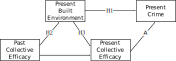
\includegraphics[width=1\linewidth]{./figure/ch2/basic_model} \caption{Theoretical model of collective efficacy, the built environment, and crime. Tested hypotheses represented as paths H1, H2, and H3.}\label{fig:basicmodel}
\end{figure}
A basic assumption of these hypotheses is that collective efficacy is negatively related to crime in the short term (path A). This is well-supported in the literature though some studies, in particular panel designs ones, find null effects, which may be a function of insufficient variation over time in collective efficacy (Lanfear, Matsueda, and Beach 2020). Testing this direct effect is not a focus of the present study but the analysis here does serve as a replication of past research. If hypotheses 1 and 2 are both supported (if paths H1 and H2 are non-zero), then criminogenic built environment features are confounders that, when omitted, exaggerate the contemporaneous effect of collective efficacy on crime. It is possible direct effects of collective efficacy on crime may be greatly, or even fully, attenuated once adjusting for features of the built environment. Even if this were the case, if hypothesis 2 is supported, it would suggest collective efficacy is still relevant to crime control, through the mechanism of control of the built environment rather than the assumed primary mechanism of informal social control. If hypothesis 3 is also supported, then adjusting for past collective efficacy in a longitudinal model does not address this spuriousness. If, however, the built environment has no effect on collective efficacy (H3 = 0), adjusting for past collective efficacy is sufficient to identify its present effect on crime by closing the path through the built environment.

While this chapter proposes a causal relationship between collective efficacy and crime via the built environment (hypotheses 1 and 2 combined), this is difficult to test. At the very least, there are four problems: (1) sequential ignorability, (2) reciprocal relationships between collective efficacy and the built environment, (3) selection in built environment features, and, less significantly, (4) task specificity of collective efficacy. I summarize these briefly here, but Appendix \ref{identification} contains a more detailed discussion.

First, collective efficacy and the built environment are not randomly assigned characteristics of neighborhoods. Establishing causal mediation---the effect of past collective efficacy on present crime via the present built environment---requires strong assumptions about sequential ignorability: assignment of both treatment (collective efficacy) and mediator (built environment) must be ignorable conditional on observed covariates (Robins and Greenland 1992). That is, one must make the assumption that all relevant covariates are included in the equations predicting both the built environment features and crime. These conditions are unlikely to hold within the complex system of an urban neighborhood. A further complication is the presence of multiple correlated mediators (i.e.~the built environment features) which makes statistical tests of mediation challenging (VanderWeele 2015). Consequently, the mediated effects are unlikely to be identified. The result of this is that we can more convincingly test for the presence of conditional direct effects---such as collective efficacy on the built environment---than for the indirect (mediated) effects---collective efficacy on crime via the built environment---which require stronger assumptions to test.

Second, it is likely that some built environment conditions foster collective efficacy, creating a positive feedback loop over time (Hypothesis 3). For example, successful removal or remediation of criminogenic features likely makes regulating the neighborhood easier by presenting fewer criminal opportunities while emboldening residents to undertake more efforts in the future as successes foster efficacy. Some features of the built environment may also increase social interaction that in turn strengthens collective efficacy (Small and Adler 2019). Endogeneity of this sort will bias estimates upward. Provided repeated observations of neighborhoods, this may be addressed with longitudinal models. In the present case, only neighborhood collective efficacy is measured at two time points, and not block-level crime or the built environment, preventing use of a conventional panel model. I address this problem by predicting built environment features using past collective efficacy, and predicting present collective efficacy with those present built environment features. This makes the assumption that the pathway from collective efficacy to the built environment operates over a longer lag than the opposite pathway, which is assumed to be approximately immediate, as residents rapidly adapt to changes in the physical environment.

Third, there is a risk of selection bias if not all neighborhoods are at risk for having certain criminogenic features of the environment. For example, an affluent and predominantly residential neighborhood may not be viewed as a potential location for a bar or liquor store, so no collective action is conceivably needed to prevent the development. Logan and Molotch (2007) describe the development of urban spaces as the result of an interaction between the political economy of metropolitan areas and neighborhood characteristics---including political capital of residents. Investment and consequent development in neighborhoods are related to current and historical structural characteristics and the relative position compared to other neighborhoods in the city (Dreier, Mollenkopf, and Swanstrom 2014; Logan and Molotch 2007). Unobserved factors such as public infrastructure, zoning, and present or anticipated land values may influence development of the built environment. For the present analysis, this is problematic if the assignment of built environment features to places is not ignorable conditional on included measures like sociodemographic structures.

There is potentially another related problem. The average treatment effect of a given feature of the built environment is not identified if, for any given strata of the population, there is a probability of zero (or one) of that feature being present. These analyses thus make the strong assumptions that assignment of built environment features is essentially random conditional on the covariates and that the probability of each feature arising is not either one or zero at any level of the covariates.

Fourth, and finally, collective efficacy is task specific (Sampson, Raudenbush, and Earls 1997). Conventional measures of collective efficacy are designed to capture informal social control capacity. However, I am concerned with residents' capacity to control the built environment, which likely occurs primarily via political action. I expect these factors will be strongly correlated, in part because one common indicator of collective efficacy is expectations residents would intervene to protect either a fire station or library---positive built environment features. That indicator describes actions to control the built environment. Nonetheless, I expect the standard measure of collective efficacy to be more strongly associated with crime directly---implicitly via informal social control---than indirectly via the built environment. This may attenuate the estimated effect of collective efficacy on the built environment.

\hypertarget{data}{%
\section{Data}\label{data}}

This analysis uses data from the community survey in the 2001 through 2003 Chicago Community Area Health Study (CCAHS) (House et al. 2011). The CCAHS was administered to a stratified, multistage sample of 3,105 adults living in Chicago. This survey provides measures of collective efficacy and the structural variables of social disorganization at the neighborhood cluster level---the primary stratification unit for the survey. These clusters were originally created for the 1995 Project in Human Development in Chicago Neighborhoods (PHDCN) to represent Chicago neighborhoods (Earls et al. 1999). Each cluster is a set of, on average, three geographically contiguous census tract. The median cluster is 0.50 square miles in area, and 90\% of clusters are between 0.19 and 1.61 square miles.\footnote{Two neighborhoods are unusually large at over 10 square miles each, due to the inclusion of large open areas: O'Hare Airport and Lake Calumet.} These clusters were constructed to maximize ecological validity using a combination of cluster analyses of census-recorded sociodemographic characteristics to ensure internal homogeneity, natural boundaries from prominent geographical features (e.g.~freeways), and local knowledge of Chicago neighborhoods (Sampson 2012:78--80; Sampson, Raudenbush, and Earls 1997:919). Hereafter I use the term neighborhood to refer to these neighborhood cluster units. For brevity, I also refer to measures from the 2001-2003 CCAHS as 2003 measures.

In line with past research in this area, I measure collective efficacy as a combination of resident expectations their neighbors would intervene against different types of deviance---but also to protect a library or fire station threatened with defunding---and perceptions of cohesion and trust---such as shared values in the neighborhood (Sampson, Raudenbush, and Earls 1997). As is common in this literature, my measure of collective efficacy is an empirical Bayes estimate derived from a multilevel measurement model that adjusts resident-perceived collective efficacy for sociodemographic characteristics of respondents and conservatively shrinks estimates toward zero where interrater reliability is lower (Sampson, Raudenbush, and Earls 1997).

Neighborhoods sociodemographic structure is a primary determinant of crime rates, and collective efficacy mediates a large portion of this relationship (Sampson, Raudenbush, and Earls 1997). To properly specify models of collective efficacy and crime, I constructed measures of neighborhood sociodemographic structure. Following past research in this area (e.g., Sampson, Raudenbush, and Earls 1997), I generate a parsimonious set of measures using an alpha-scoring oblique factor rotation of nine year 2000 census indicators from the Longitudinal Tract Data Base (LTDB) (Logan, Xu, and Stults 2014). The LTDB normalizes census tract boundaries over time to ensure measures in longitudinal studies describe the same units over time.\footnote{Chicago is a unique city, however, in that its census tract boundaries have remained largely fixed since the 1920s. Use of non-normalized data likely will produce identical results in Chicago.} Despite being conducted in 2001-2003, the CCAHS data is identified to year 1990 census boundaries. The LTDB was used to ensure the survey and census data describe the same geographical units. The indicators were chosen to match those used by Sampson, Raudenbush, and Earls (1997) to operationalize 1990 neighborhood social-structural characteristics, though one of these indicators (percent families on public assistance) was not available in the LTDB.\footnote{I calculated 1990 factor scores without this same indicator and compared them to those calculated by Sampson, Raudenbush, and Earls (1997). All three factors exhibit correlations greater than .95 with those from Sampson, Raudenbush, and Earls (1997).} Based on the factors each indicator loads on, I label the factors disadvantage, stability, and Hispanic / immigrant population. These factors are analogous to the classic structural antecedents of social disorganization and its modern derivatives (Bursik and Grasmick 1993; Shaw and McKay {[}1969{]} 1942). See Appendix \ref{measures} for a list of indicators and their factor loadings.

The CCAHS also provides systematic social observation (SSO) measures of a random sample of census blocks within each neighborhood cluster---almost exclusively the same blocks in which respondents resided. The SSO for the CCAHS was conducted by survey interviewers walking the perimeter of the sampled block twice and recording what they observe on each block face via a checklist. A block face is a single side of the street between two intersections that form corners of a block; a rectangular block, for example, has four block faces. Observers recorded data for block faces on the focal block, as well as block faces on adjacent blocks that face the focal block. In this case, a square block would have eight block face observations consisting of its own four block faces and the four faces across each street adjacent to the block. The indicators recorded cover a broad range of features describing the health hazards, the built environment, and disorder (see House et al. 2011). The SSO for the CCAHS covers all 343 neighborhood clusters, however only 1,641 of Chicago's approximately 20,000 census blocks are represented. Figure \ref{fig:blocksample} depicts the sampled blocks and neighborhood clusters. Note that most blocks are isolated or adjacent to few other blocks.
\begin{figure}

{\centering 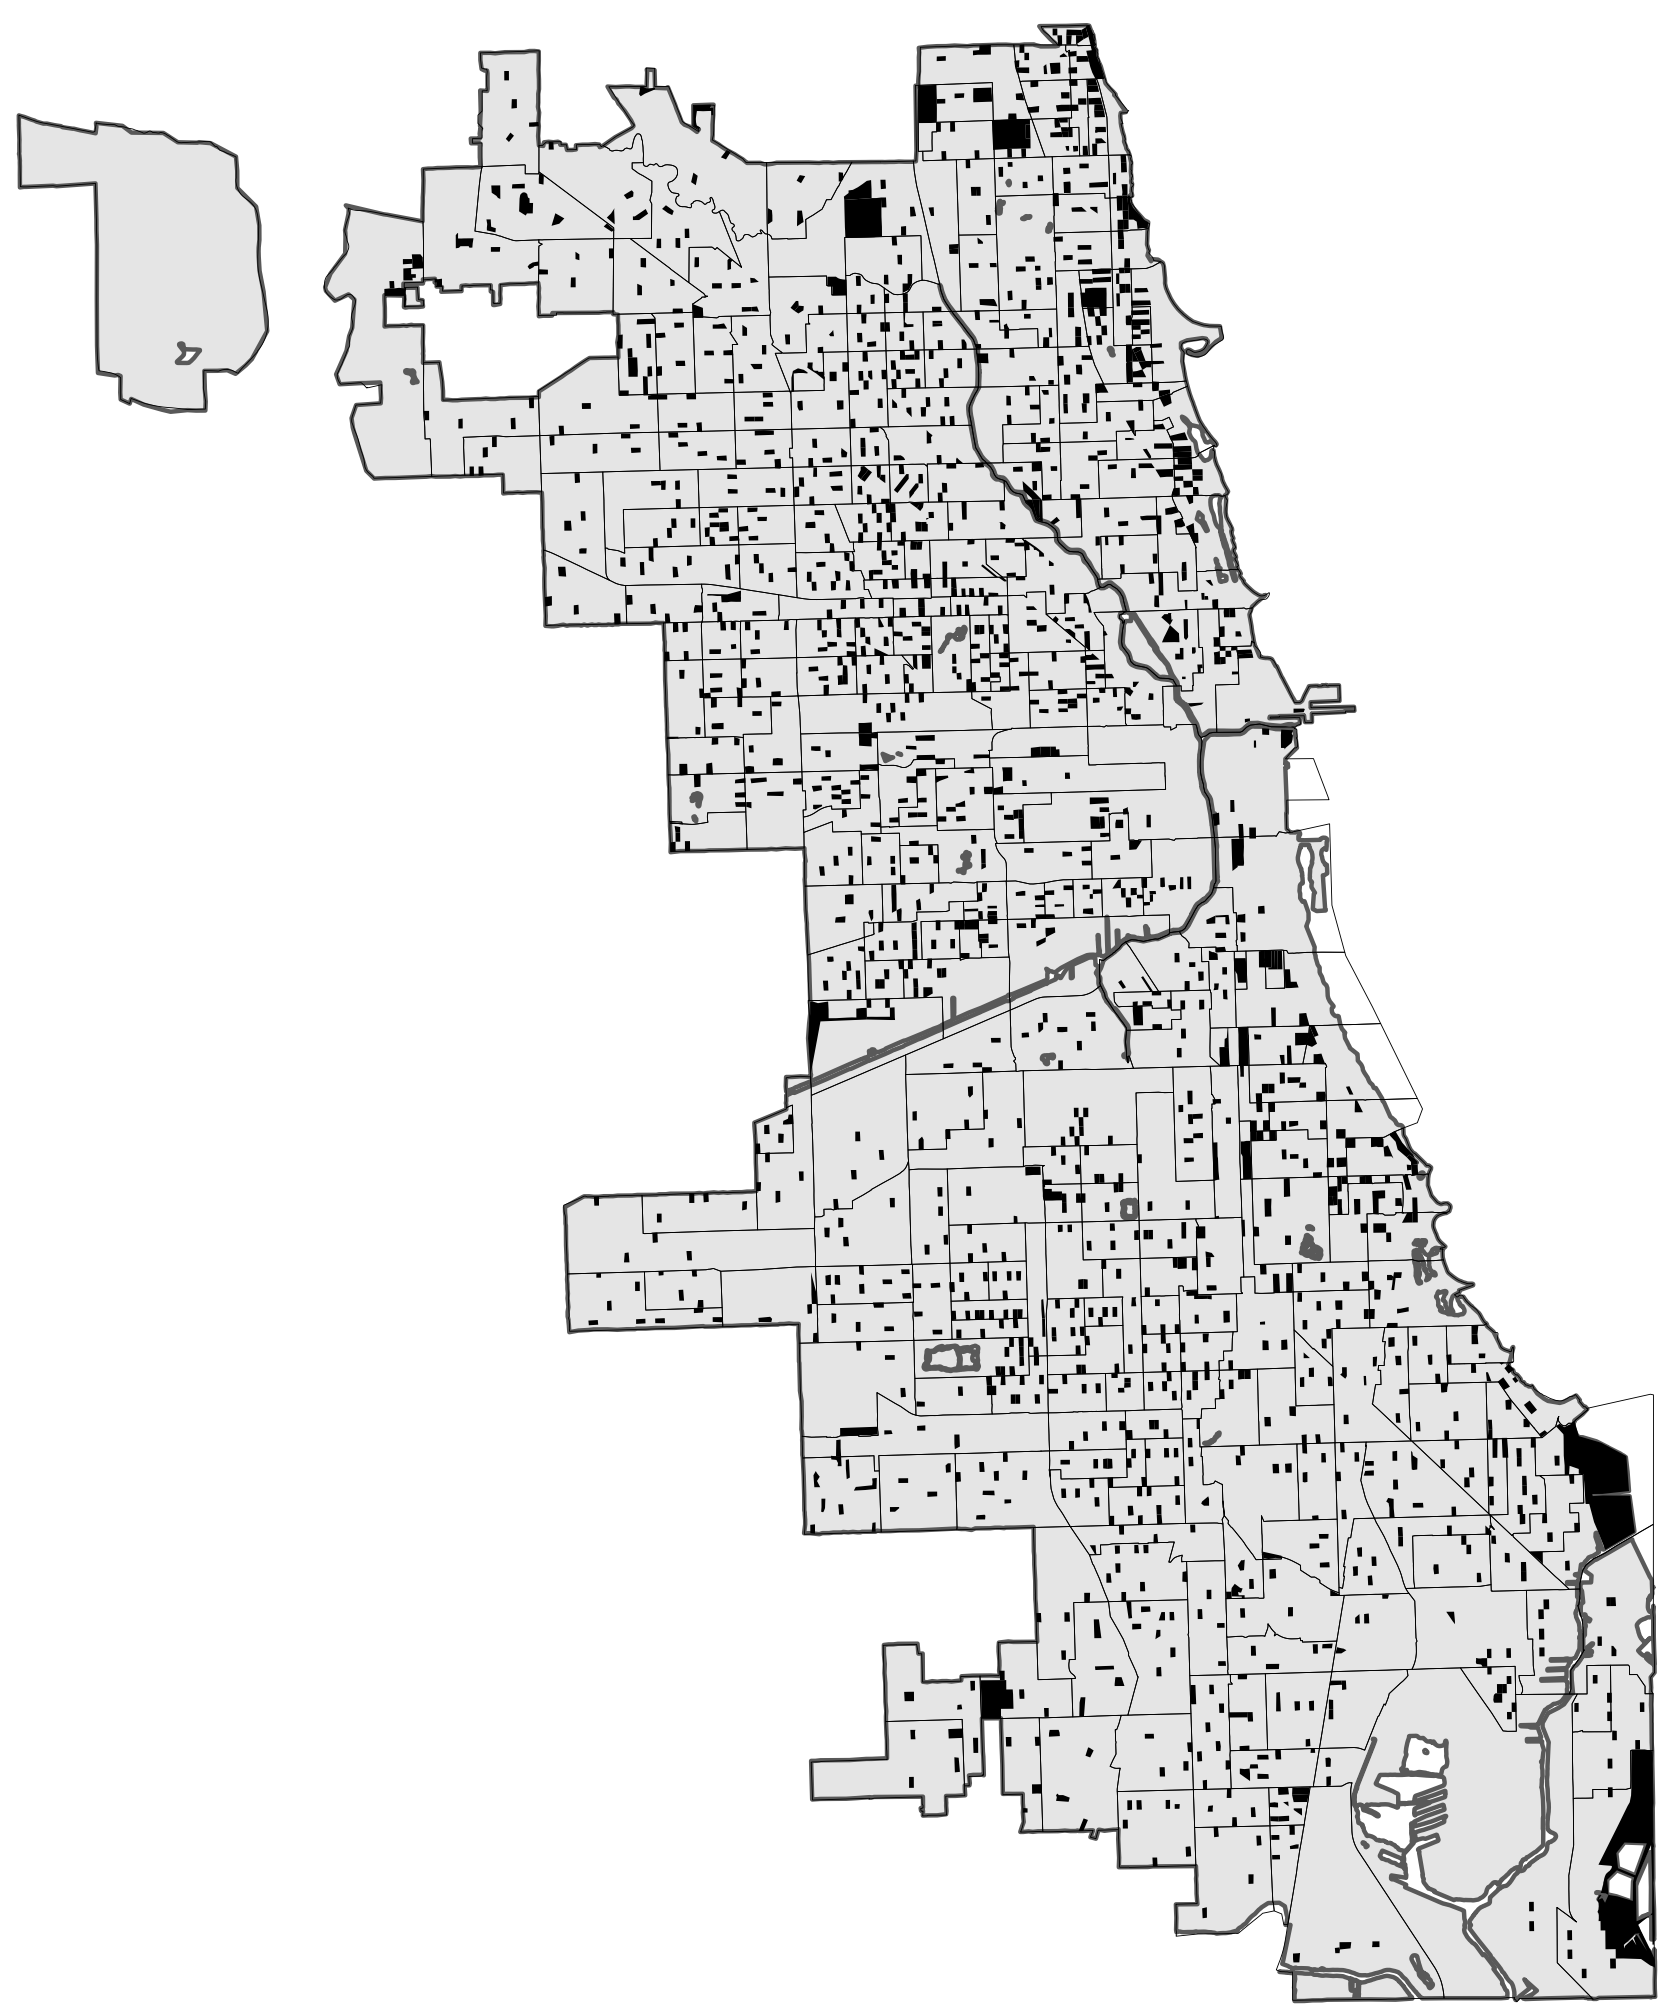
\includegraphics[width=0.93\linewidth]{./figure/ch2/boundary_map} 

}

\caption{Map of census blocks sampled in 2001-2003 Chicago Community Adult Health Study. Sampled blocks are filled black shapes. Neighborhood clusters are outlines. }\label{fig:blocksample}
\end{figure}
From the SSO, I obtain measures of all built environment features: abandoned buildings, bars, commercial destinations, liquor stores, mixed land use, parking lots, recreation facilities, and vacant lots. All built environment measures are proportions of block faces on and surrounding the census block which have that feature present. A proportion of one for abandoned buildings, for example, means that every block face on and around that block has at least one abandoned building. I exclude measures of commercial and residential security---such as bars on windows---which are protective measures undertaken by property owners that are likely to be endogenous to crime rates. My focus here is on community control of built environment features that provide opportunities rather than individual protective measures.

It is important to note that these features are likely spread across a continuum of perceived desirability by residents. Abandoned buildings have no positive functions for any neighborhood residents, with the possible exception of property owners awaiting rising values to redevelop or sell. In contrast, most commercial destinations and recreation facilities likely provide valuable amenities to the neighborhood. The degree to which collective efficacy is associated with the presence of these features is likely governed by the perceived balance of positive and negative impacts they make to the neighborhood. That is, even if a particular built environment feature---like a local park---is associated with crime, residents may not advocate for the removal of the property if it provides use value to the neighborhood that outweighs the cost of crime. In this way I diverge from studies which focus on the criminogenic effects and control only of ``unpopular places'' (Wilcox and Eck 2011). It may be the case that many features are comparably criminogenic, but removal efforts are concentrated on those features perceived as particularly undesirable or unambiguously problematic.

For an analysis of the impact of past collective efficacy on the built environment, I construct a past collective efficacy measure from the 1995 PHDCN community survey (PHDCN-CS). I estimate this measure using the same multilevel approach as for the CCAHS. The PHDCN-CS is similar to the CCAHS's community survey but produces more precise estimates of neighborhood social structures due to its larger sample size (N=8,782). The PHDCN SSO is not used for block-level analyses because it was conducted in only 80 neighborhood clusters and no block-level identifiers are available to link those blocks across surveys.

The neighborhood and block measures were linked to publicly-available geocoded Chicago Police Department crime data from the three years after the CCAHS (2004-2006) to obtain block-level counts of crime incidents ({Chicago Police Department} 2020). A three-year span was used because serious crimes are relatively rare at the block level---using multiple years reduces the influence of idiosyncratic variation. I consider five forms of crime: (1) homicide, (2) assaults with a gun, (3) robbery, (4) any violent crime (defined as 1 through 3 plus assaults without a gun), and (5) any property crime (defined as burglary and theft). These forms of crime were chosen for two reasons. First, they are direct contact predatory violations likely to be particularly sensitive to different opportunities structured by the built environment. Second, accuracy of reporting tends to be higher for more serious crimes such as homicide and gun violence. These geocoded crime data are only publicly available from 2001 onward, which prevents constructing a complete block-level panel dataset even if the blocks in the 80 clusters of the PHDCN with built environment measures could be identified. The police records are also only geoidentified to the city block level, preventing the use of more granular geographic units sometimes used in the situational opportunity literature like properties and street segments (e.g., Sherman, Gartin, and Buerger 1989; Weisburd, Groff, and Yang 2012).

Lastly, census data from 2000 were used to adjust for block-level population density. Despite being collected in 2001-2003, CCAHS blocks were identified using 1990 census block boundaries to facilitate linking to the 1995 PHDCN. Consequently, 2000 block populations were areal weighted to the 1990 boundaries where boundaries changed across decennial censuses. Areal weighting is a process in which values describing one geographic area are assigned to another geographic area in proportion to the area of their intersection, under the assumption the values of interest are distributed uniformly in space. These resulting population values were then divided by block area to arrive at a block population density. This is a block-level analog of the tract-level normalization process for the LTDB which was used to construct neighborhood-level measures. The resulting final analytical data describe 1,641 blocks nested in 343 neighborhoods. Table \ref{tab:bedescrip} presents descriptive statistics for these data.

\providecommand{\docline}[3]{\noalign{\global\setlength{\arrayrulewidth}{#1}}\arrayrulecolor[HTML]{#2}\cline{#3}}

\setlength{\tabcolsep}{2pt}

\renewcommand*{\arraystretch}{1}
\begin{longtable}[c]{ccccccc}

\caption{\label{tab:bedescrip} Descriptive Statistics}\label{tab:unnamed-chunk-1}\\

\hhline{>{\arrayrulecolor[HTML]{000000}\global\arrayrulewidth=1pt}->{\arrayrulecolor[HTML]{000000}\global\arrayrulewidth=1pt}->{\arrayrulecolor[HTML]{000000}\global\arrayrulewidth=1pt}->{\arrayrulecolor[HTML]{000000}\global\arrayrulewidth=1pt}->{\arrayrulecolor[HTML]{000000}\global\arrayrulewidth=1pt}->{\arrayrulecolor[HTML]{000000}\global\arrayrulewidth=1pt}->{\arrayrulecolor[HTML]{000000}\global\arrayrulewidth=1pt}-}

\multicolumn{1}{!{\color[HTML]{000000}\vrule width 0pt}>{}l}{\fontsize{11}{11}\selectfont{\textcolor[HTML]{000000}{\global\setmainfont{Latin Modern Roman}}}} & \multicolumn{1}{!{\color[HTML]{000000}\vrule width 0pt}>{}l}{\fontsize{11}{11}\selectfont{\textcolor[HTML]{000000}{\global\setmainfont{Latin Modern Roman}Measure}}} & \multicolumn{1}{!{\color[HTML]{000000}\vrule width 0pt}>{}c}{\fontsize{11}{11}\selectfont{\textcolor[HTML]{000000}{\global\setmainfont{Latin Modern Roman}Mean}}} & \multicolumn{1}{!{\color[HTML]{000000}\vrule width 0pt}>{}c}{\fontsize{11}{11}\selectfont{\textcolor[HTML]{000000}{\global\setmainfont{Latin Modern Roman}SD}}} & \multicolumn{1}{!{\color[HTML]{000000}\vrule width 0pt}>{}c}{\fontsize{11}{11}\selectfont{\textcolor[HTML]{000000}{\global\setmainfont{Latin Modern Roman}Min}}} & \multicolumn{1}{!{\color[HTML]{000000}\vrule width 0pt}>{}c}{\fontsize{11}{11}\selectfont{\textcolor[HTML]{000000}{\global\setmainfont{Latin Modern Roman}Density}}} & \multicolumn{1}{!{\color[HTML]{000000}\vrule width 0pt}>{}c!{\color[HTML]{000000}\vrule width 0pt}}{\fontsize{11}{11}\selectfont{\textcolor[HTML]{000000}{\global\setmainfont{Latin Modern Roman}Max}}} \\

\noalign{\global\setlength{\arrayrulewidth}{0.5pt}}\arrayrulecolor[HTML]{000000}\cline{1-7}

\endfirsthead

\hhline{>{\arrayrulecolor[HTML]{000000}\global\arrayrulewidth=1pt}->{\arrayrulecolor[HTML]{000000}\global\arrayrulewidth=1pt}->{\arrayrulecolor[HTML]{000000}\global\arrayrulewidth=1pt}->{\arrayrulecolor[HTML]{000000}\global\arrayrulewidth=1pt}->{\arrayrulecolor[HTML]{000000}\global\arrayrulewidth=1pt}->{\arrayrulecolor[HTML]{000000}\global\arrayrulewidth=1pt}->{\arrayrulecolor[HTML]{000000}\global\arrayrulewidth=1pt}-}

\multicolumn{1}{!{\color[HTML]{000000}\vrule width 0pt}>{}l}{\fontsize{11}{11}\selectfont{\textcolor[HTML]{000000}{\global\setmainfont{Latin Modern Roman}}}} & \multicolumn{1}{!{\color[HTML]{000000}\vrule width 0pt}>{}l}{\fontsize{11}{11}\selectfont{\textcolor[HTML]{000000}{\global\setmainfont{Latin Modern Roman}Measure}}} & \multicolumn{1}{!{\color[HTML]{000000}\vrule width 0pt}>{}c}{\fontsize{11}{11}\selectfont{\textcolor[HTML]{000000}{\global\setmainfont{Latin Modern Roman}Mean}}} & \multicolumn{1}{!{\color[HTML]{000000}\vrule width 0pt}>{}c}{\fontsize{11}{11}\selectfont{\textcolor[HTML]{000000}{\global\setmainfont{Latin Modern Roman}SD}}} & \multicolumn{1}{!{\color[HTML]{000000}\vrule width 0pt}>{}c}{\fontsize{11}{11}\selectfont{\textcolor[HTML]{000000}{\global\setmainfont{Latin Modern Roman}Min}}} & \multicolumn{1}{!{\color[HTML]{000000}\vrule width 0pt}>{}c}{\fontsize{11}{11}\selectfont{\textcolor[HTML]{000000}{\global\setmainfont{Latin Modern Roman}Density}}} & \multicolumn{1}{!{\color[HTML]{000000}\vrule width 0pt}>{}c!{\color[HTML]{000000}\vrule width 0pt}}{\fontsize{11}{11}\selectfont{\textcolor[HTML]{000000}{\global\setmainfont{Latin Modern Roman}Max}}} \\

\noalign{\global\setlength{\arrayrulewidth}{0.5pt}}\arrayrulecolor[HTML]{000000}\cline{1-7}\endhead



\multicolumn{7}{!{\color[HTML]{000000}\vrule width 0pt}>{}l}{\fontsize{11}{11}\selectfont{\textcolor[HTML]{000000}{\global\setmainfont{Latin Modern Roman}Neighborhood (N=343)}}} \\





\multicolumn{1}{!{\color[HTML]{000000}\vrule width 0pt}>{}l}{\fontsize{11}{11}\selectfont{\textcolor[HTML]{000000}{\global\setmainfont{Latin Modern Roman}}}} & \multicolumn{1}{!{\color[HTML]{000000}\vrule width 0pt}>{}l}{\fontsize{11}{11}\selectfont{\textcolor[HTML]{000000}{\global\setmainfont{Latin Modern Roman}Collective Efficacy (2003)}}} & \multicolumn{1}{!{\color[HTML]{000000}\vrule width 0pt}>{}c}{\fontsize{11}{11}\selectfont{\textcolor[HTML]{000000}{\global\setmainfont{Latin Modern Roman}0.00}}} & \multicolumn{1}{!{\color[HTML]{000000}\vrule width 0pt}>{}c}{\fontsize{11}{11}\selectfont{\textcolor[HTML]{000000}{\global\setmainfont{Latin Modern Roman}1.00}}} & \multicolumn{1}{!{\color[HTML]{000000}\vrule width 0pt}>{}c}{\fontsize{11}{11}\selectfont{\textcolor[HTML]{000000}{\global\setmainfont{Latin Modern Roman}-3.64}}} & \multicolumn{1}{!{\color[HTML]{000000}\vrule width 0pt}>{}c}{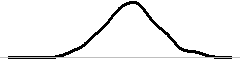
\includegraphics[width=0.8in, height=0.2in]{thesis_files/figure-latex/unnamed-chunk-1-1.png}} & \multicolumn{1}{!{\color[HTML]{000000}\vrule width 0pt}>{}c!{\color[HTML]{000000}\vrule width 0pt}}{\fontsize{11}{11}\selectfont{\textcolor[HTML]{000000}{\global\setmainfont{Latin Modern Roman}2.81}}} \\





\multicolumn{1}{!{\color[HTML]{000000}\vrule width 0pt}>{}l}{\fontsize{11}{11}\selectfont{\textcolor[HTML]{000000}{\global\setmainfont{Latin Modern Roman}}}} & \multicolumn{1}{!{\color[HTML]{000000}\vrule width 0pt}>{}l}{\fontsize{11}{11}\selectfont{\textcolor[HTML]{000000}{\global\setmainfont{Latin Modern Roman}Collective Efficacy (1995)}}} & \multicolumn{1}{!{\color[HTML]{000000}\vrule width 0pt}>{}c}{\fontsize{11}{11}\selectfont{\textcolor[HTML]{000000}{\global\setmainfont{Latin Modern Roman}0.00}}} & \multicolumn{1}{!{\color[HTML]{000000}\vrule width 0pt}>{}c}{\fontsize{11}{11}\selectfont{\textcolor[HTML]{000000}{\global\setmainfont{Latin Modern Roman}1.00}}} & \multicolumn{1}{!{\color[HTML]{000000}\vrule width 0pt}>{}c}{\fontsize{11}{11}\selectfont{\textcolor[HTML]{000000}{\global\setmainfont{Latin Modern Roman}-2.93}}} & \multicolumn{1}{!{\color[HTML]{000000}\vrule width 0pt}>{}c}{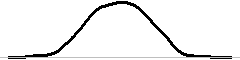
\includegraphics[width=0.8in, height=0.2in]{thesis_files/figure-latex/unnamed-chunk-1-2.png}} & \multicolumn{1}{!{\color[HTML]{000000}\vrule width 0pt}>{}c!{\color[HTML]{000000}\vrule width 0pt}}{\fontsize{11}{11}\selectfont{\textcolor[HTML]{000000}{\global\setmainfont{Latin Modern Roman}3.00}}} \\





\multicolumn{1}{!{\color[HTML]{000000}\vrule width 0pt}>{}l}{\fontsize{11}{11}\selectfont{\textcolor[HTML]{000000}{\global\setmainfont{Latin Modern Roman}}}} & \multicolumn{1}{!{\color[HTML]{000000}\vrule width 0pt}>{}l}{\fontsize{11}{11}\selectfont{\textcolor[HTML]{000000}{\global\setmainfont{Latin Modern Roman}Disadvantage}}} & \multicolumn{1}{!{\color[HTML]{000000}\vrule width 0pt}>{}c}{\fontsize{11}{11}\selectfont{\textcolor[HTML]{000000}{\global\setmainfont{Latin Modern Roman}0.00}}} & \multicolumn{1}{!{\color[HTML]{000000}\vrule width 0pt}>{}c}{\fontsize{11}{11}\selectfont{\textcolor[HTML]{000000}{\global\setmainfont{Latin Modern Roman}1.00}}} & \multicolumn{1}{!{\color[HTML]{000000}\vrule width 0pt}>{}c}{\fontsize{11}{11}\selectfont{\textcolor[HTML]{000000}{\global\setmainfont{Latin Modern Roman}-2.35}}} & \multicolumn{1}{!{\color[HTML]{000000}\vrule width 0pt}>{}c}{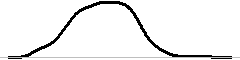
\includegraphics[width=0.8in, height=0.2in]{thesis_files/figure-latex/unnamed-chunk-1-3.png}} & \multicolumn{1}{!{\color[HTML]{000000}\vrule width 0pt}>{}c!{\color[HTML]{000000}\vrule width 0pt}}{\fontsize{11}{11}\selectfont{\textcolor[HTML]{000000}{\global\setmainfont{Latin Modern Roman}3.45}}} \\





\multicolumn{1}{!{\color[HTML]{000000}\vrule width 0pt}>{}l}{\fontsize{11}{11}\selectfont{\textcolor[HTML]{000000}{\global\setmainfont{Latin Modern Roman}}}} & \multicolumn{1}{!{\color[HTML]{000000}\vrule width 0pt}>{}l}{\fontsize{11}{11}\selectfont{\textcolor[HTML]{000000}{\global\setmainfont{Latin Modern Roman}Stability}}} & \multicolumn{1}{!{\color[HTML]{000000}\vrule width 0pt}>{}c}{\fontsize{11}{11}\selectfont{\textcolor[HTML]{000000}{\global\setmainfont{Latin Modern Roman}0.00}}} & \multicolumn{1}{!{\color[HTML]{000000}\vrule width 0pt}>{}c}{\fontsize{11}{11}\selectfont{\textcolor[HTML]{000000}{\global\setmainfont{Latin Modern Roman}1.00}}} & \multicolumn{1}{!{\color[HTML]{000000}\vrule width 0pt}>{}c}{\fontsize{11}{11}\selectfont{\textcolor[HTML]{000000}{\global\setmainfont{Latin Modern Roman}-2.39}}} & \multicolumn{1}{!{\color[HTML]{000000}\vrule width 0pt}>{}c}{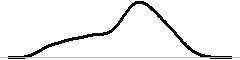
\includegraphics[width=0.8in, height=0.2in]{thesis_files/figure-latex/unnamed-chunk-1-4.png}} & \multicolumn{1}{!{\color[HTML]{000000}\vrule width 0pt}>{}c!{\color[HTML]{000000}\vrule width 0pt}}{\fontsize{11}{11}\selectfont{\textcolor[HTML]{000000}{\global\setmainfont{Latin Modern Roman}2.04}}} \\





\multicolumn{1}{!{\color[HTML]{000000}\vrule width 0pt}>{}l}{\fontsize{11}{11}\selectfont{\textcolor[HTML]{000000}{\global\setmainfont{Latin Modern Roman}}}} & \multicolumn{1}{!{\color[HTML]{000000}\vrule width 0pt}>{}l}{\fontsize{11}{11}\selectfont{\textcolor[HTML]{000000}{\global\setmainfont{Latin Modern Roman}Hispanic/Immigrant}}} & \multicolumn{1}{!{\color[HTML]{000000}\vrule width 0pt}>{}c}{\fontsize{11}{11}\selectfont{\textcolor[HTML]{000000}{\global\setmainfont{Latin Modern Roman}0.00}}} & \multicolumn{1}{!{\color[HTML]{000000}\vrule width 0pt}>{}c}{\fontsize{11}{11}\selectfont{\textcolor[HTML]{000000}{\global\setmainfont{Latin Modern Roman}1.00}}} & \multicolumn{1}{!{\color[HTML]{000000}\vrule width 0pt}>{}c}{\fontsize{11}{11}\selectfont{\textcolor[HTML]{000000}{\global\setmainfont{Latin Modern Roman}-1.60}}} & \multicolumn{1}{!{\color[HTML]{000000}\vrule width 0pt}>{}c}{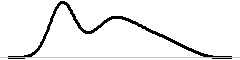
\includegraphics[width=0.8in, height=0.2in]{thesis_files/figure-latex/unnamed-chunk-1-5.png}} & \multicolumn{1}{!{\color[HTML]{000000}\vrule width 0pt}>{}c!{\color[HTML]{000000}\vrule width 0pt}}{\fontsize{11}{11}\selectfont{\textcolor[HTML]{000000}{\global\setmainfont{Latin Modern Roman}2.30}}} \\





\multicolumn{1}{!{\color[HTML]{000000}\vrule width 0pt}>{}l}{\fontsize{11}{11}\selectfont{\textcolor[HTML]{000000}{\global\setmainfont{Latin Modern Roman}}}} & \multicolumn{1}{!{\color[HTML]{000000}\vrule width 0pt}>{}l}{\fontsize{11}{11}\selectfont{\textcolor[HTML]{000000}{\global\setmainfont{Latin Modern Roman}Density (Neighborhood)}}} & \multicolumn{1}{!{\color[HTML]{000000}\vrule width 0pt}>{}c}{\fontsize{11}{11}\selectfont{\textcolor[HTML]{000000}{\global\setmainfont{Latin Modern Roman}7.09}}} & \multicolumn{1}{!{\color[HTML]{000000}\vrule width 0pt}>{}c}{\fontsize{11}{11}\selectfont{\textcolor[HTML]{000000}{\global\setmainfont{Latin Modern Roman}4.37}}} & \multicolumn{1}{!{\color[HTML]{000000}\vrule width 0pt}>{}c}{\fontsize{11}{11}\selectfont{\textcolor[HTML]{000000}{\global\setmainfont{Latin Modern Roman}0.18}}} & \multicolumn{1}{!{\color[HTML]{000000}\vrule width 0pt}>{}c}{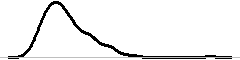
\includegraphics[width=0.8in, height=0.2in]{thesis_files/figure-latex/unnamed-chunk-1-6.png}} & \multicolumn{1}{!{\color[HTML]{000000}\vrule width 0pt}>{}c!{\color[HTML]{000000}\vrule width 0pt}}{\fontsize{11}{11}\selectfont{\textcolor[HTML]{000000}{\global\setmainfont{Latin Modern Roman}31.61}}} \\





\multicolumn{7}{!{\color[HTML]{000000}\vrule width 0pt}>{}l}{\fontsize{11}{11}\selectfont{\textcolor[HTML]{000000}{\global\setmainfont{Latin Modern Roman}Block (N=1,641)}}} \\





\multicolumn{1}{!{\color[HTML]{000000}\vrule width 0pt}>{}l}{\fontsize{11}{11}\selectfont{\textcolor[HTML]{000000}{\global\setmainfont{Latin Modern Roman}}}} & \multicolumn{1}{!{\color[HTML]{000000}\vrule width 0pt}>{}l}{\fontsize{11}{11}\selectfont{\textcolor[HTML]{000000}{\global\setmainfont{Latin Modern Roman}Homicide}}} & \multicolumn{1}{!{\color[HTML]{000000}\vrule width 0pt}>{}c}{\fontsize{11}{11}\selectfont{\textcolor[HTML]{000000}{\global\setmainfont{Latin Modern Roman}0.10}}} & \multicolumn{1}{!{\color[HTML]{000000}\vrule width 0pt}>{}c}{\fontsize{11}{11}\selectfont{\textcolor[HTML]{000000}{\global\setmainfont{Latin Modern Roman}0.35}}} & \multicolumn{1}{!{\color[HTML]{000000}\vrule width 0pt}>{}c}{\fontsize{11}{11}\selectfont{\textcolor[HTML]{000000}{\global\setmainfont{Latin Modern Roman}0.00}}} & \multicolumn{1}{!{\color[HTML]{000000}\vrule width 0pt}>{}c}{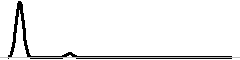
\includegraphics[width=0.8in, height=0.2in]{thesis_files/figure-latex/unnamed-chunk-1-7.png}} & \multicolumn{1}{!{\color[HTML]{000000}\vrule width 0pt}>{}c!{\color[HTML]{000000}\vrule width 0pt}}{\fontsize{11}{11}\selectfont{\textcolor[HTML]{000000}{\global\setmainfont{Latin Modern Roman}4.00}}} \\





\multicolumn{1}{!{\color[HTML]{000000}\vrule width 0pt}>{}l}{\fontsize{11}{11}\selectfont{\textcolor[HTML]{000000}{\global\setmainfont{Latin Modern Roman}}}} & \multicolumn{1}{!{\color[HTML]{000000}\vrule width 0pt}>{}l}{\fontsize{11}{11}\selectfont{\textcolor[HTML]{000000}{\global\setmainfont{Latin Modern Roman}Gun Assault}}} & \multicolumn{1}{!{\color[HTML]{000000}\vrule width 0pt}>{}c}{\fontsize{11}{11}\selectfont{\textcolor[HTML]{000000}{\global\setmainfont{Latin Modern Roman}0.98}}} & \multicolumn{1}{!{\color[HTML]{000000}\vrule width 0pt}>{}c}{\fontsize{11}{11}\selectfont{\textcolor[HTML]{000000}{\global\setmainfont{Latin Modern Roman}1.69}}} & \multicolumn{1}{!{\color[HTML]{000000}\vrule width 0pt}>{}c}{\fontsize{11}{11}\selectfont{\textcolor[HTML]{000000}{\global\setmainfont{Latin Modern Roman}0.00}}} & \multicolumn{1}{!{\color[HTML]{000000}\vrule width 0pt}>{}c}{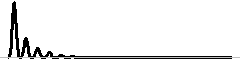
\includegraphics[width=0.8in, height=0.2in]{thesis_files/figure-latex/unnamed-chunk-1-8.png}} & \multicolumn{1}{!{\color[HTML]{000000}\vrule width 0pt}>{}c!{\color[HTML]{000000}\vrule width 0pt}}{\fontsize{11}{11}\selectfont{\textcolor[HTML]{000000}{\global\setmainfont{Latin Modern Roman}18.00}}} \\





\multicolumn{1}{!{\color[HTML]{000000}\vrule width 0pt}>{}l}{\fontsize{11}{11}\selectfont{\textcolor[HTML]{000000}{\global\setmainfont{Latin Modern Roman}}}} & \multicolumn{1}{!{\color[HTML]{000000}\vrule width 0pt}>{}l}{\fontsize{11}{11}\selectfont{\textcolor[HTML]{000000}{\global\setmainfont{Latin Modern Roman}Robbery}}} & \multicolumn{1}{!{\color[HTML]{000000}\vrule width 0pt}>{}c}{\fontsize{11}{11}\selectfont{\textcolor[HTML]{000000}{\global\setmainfont{Latin Modern Roman}3.18}}} & \multicolumn{1}{!{\color[HTML]{000000}\vrule width 0pt}>{}c}{\fontsize{11}{11}\selectfont{\textcolor[HTML]{000000}{\global\setmainfont{Latin Modern Roman}4.39}}} & \multicolumn{1}{!{\color[HTML]{000000}\vrule width 0pt}>{}c}{\fontsize{11}{11}\selectfont{\textcolor[HTML]{000000}{\global\setmainfont{Latin Modern Roman}0.00}}} & \multicolumn{1}{!{\color[HTML]{000000}\vrule width 0pt}>{}c}{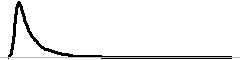
\includegraphics[width=0.8in, height=0.2in]{thesis_files/figure-latex/unnamed-chunk-1-9.png}} & \multicolumn{1}{!{\color[HTML]{000000}\vrule width 0pt}>{}c!{\color[HTML]{000000}\vrule width 0pt}}{\fontsize{11}{11}\selectfont{\textcolor[HTML]{000000}{\global\setmainfont{Latin Modern Roman}44.00}}} \\





\multicolumn{1}{!{\color[HTML]{000000}\vrule width 0pt}>{}l}{\fontsize{11}{11}\selectfont{\textcolor[HTML]{000000}{\global\setmainfont{Latin Modern Roman}}}} & \multicolumn{1}{!{\color[HTML]{000000}\vrule width 0pt}>{}l}{\fontsize{11}{11}\selectfont{\textcolor[HTML]{000000}{\global\setmainfont{Latin Modern Roman}Violent}}} & \multicolumn{1}{!{\color[HTML]{000000}\vrule width 0pt}>{}c}{\fontsize{11}{11}\selectfont{\textcolor[HTML]{000000}{\global\setmainfont{Latin Modern Roman}6.58}}} & \multicolumn{1}{!{\color[HTML]{000000}\vrule width 0pt}>{}c}{\fontsize{11}{11}\selectfont{\textcolor[HTML]{000000}{\global\setmainfont{Latin Modern Roman}8.57}}} & \multicolumn{1}{!{\color[HTML]{000000}\vrule width 0pt}>{}c}{\fontsize{11}{11}\selectfont{\textcolor[HTML]{000000}{\global\setmainfont{Latin Modern Roman}0.00}}} & \multicolumn{1}{!{\color[HTML]{000000}\vrule width 0pt}>{}c}{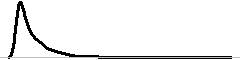
\includegraphics[width=0.8in, height=0.2in]{thesis_files/figure-latex/unnamed-chunk-1-10.png}} & \multicolumn{1}{!{\color[HTML]{000000}\vrule width 0pt}>{}c!{\color[HTML]{000000}\vrule width 0pt}}{\fontsize{11}{11}\selectfont{\textcolor[HTML]{000000}{\global\setmainfont{Latin Modern Roman}85.00}}} \\





\multicolumn{1}{!{\color[HTML]{000000}\vrule width 0pt}>{}l}{\fontsize{11}{11}\selectfont{\textcolor[HTML]{000000}{\global\setmainfont{Latin Modern Roman}}}} & \multicolumn{1}{!{\color[HTML]{000000}\vrule width 0pt}>{}l}{\fontsize{11}{11}\selectfont{\textcolor[HTML]{000000}{\global\setmainfont{Latin Modern Roman}Property}}} & \multicolumn{1}{!{\color[HTML]{000000}\vrule width 0pt}>{}c}{\fontsize{11}{11}\selectfont{\textcolor[HTML]{000000}{\global\setmainfont{Latin Modern Roman}20.33}}} & \multicolumn{1}{!{\color[HTML]{000000}\vrule width 0pt}>{}c}{\fontsize{11}{11}\selectfont{\textcolor[HTML]{000000}{\global\setmainfont{Latin Modern Roman}24.62}}} & \multicolumn{1}{!{\color[HTML]{000000}\vrule width 0pt}>{}c}{\fontsize{11}{11}\selectfont{\textcolor[HTML]{000000}{\global\setmainfont{Latin Modern Roman}0.00}}} & \multicolumn{1}{!{\color[HTML]{000000}\vrule width 0pt}>{}c}{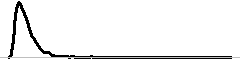
\includegraphics[width=0.8in, height=0.2in]{thesis_files/figure-latex/unnamed-chunk-1-11.png}} & \multicolumn{1}{!{\color[HTML]{000000}\vrule width 0pt}>{}c!{\color[HTML]{000000}\vrule width 0pt}}{\fontsize{11}{11}\selectfont{\textcolor[HTML]{000000}{\global\setmainfont{Latin Modern Roman}315.00}}} \\





\multicolumn{1}{!{\color[HTML]{000000}\vrule width 0pt}>{}l}{\fontsize{11}{11}\selectfont{\textcolor[HTML]{000000}{\global\setmainfont{Latin Modern Roman}}}} & \multicolumn{1}{!{\color[HTML]{000000}\vrule width 0pt}>{}l}{\fontsize{11}{11}\selectfont{\textcolor[HTML]{000000}{\global\setmainfont{Latin Modern Roman}Abandoned}}} & \multicolumn{1}{!{\color[HTML]{000000}\vrule width 0pt}>{}c}{\fontsize{11}{11}\selectfont{\textcolor[HTML]{000000}{\global\setmainfont{Latin Modern Roman}0.12}}} & \multicolumn{1}{!{\color[HTML]{000000}\vrule width 0pt}>{}c}{\fontsize{11}{11}\selectfont{\textcolor[HTML]{000000}{\global\setmainfont{Latin Modern Roman}0.21}}} & \multicolumn{1}{!{\color[HTML]{000000}\vrule width 0pt}>{}c}{\fontsize{11}{11}\selectfont{\textcolor[HTML]{000000}{\global\setmainfont{Latin Modern Roman}0.00}}} & \multicolumn{1}{!{\color[HTML]{000000}\vrule width 0pt}>{}c}{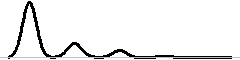
\includegraphics[width=0.8in, height=0.2in]{thesis_files/figure-latex/unnamed-chunk-1-12.png}} & \multicolumn{1}{!{\color[HTML]{000000}\vrule width 0pt}>{}c!{\color[HTML]{000000}\vrule width 0pt}}{\fontsize{11}{11}\selectfont{\textcolor[HTML]{000000}{\global\setmainfont{Latin Modern Roman}1.00}}} \\





\multicolumn{1}{!{\color[HTML]{000000}\vrule width 0pt}>{}l}{\fontsize{11}{11}\selectfont{\textcolor[HTML]{000000}{\global\setmainfont{Latin Modern Roman}}}} & \multicolumn{1}{!{\color[HTML]{000000}\vrule width 0pt}>{}l}{\fontsize{11}{11}\selectfont{\textcolor[HTML]{000000}{\global\setmainfont{Latin Modern Roman}Bars}}} & \multicolumn{1}{!{\color[HTML]{000000}\vrule width 0pt}>{}c}{\fontsize{11}{11}\selectfont{\textcolor[HTML]{000000}{\global\setmainfont{Latin Modern Roman}0.05}}} & \multicolumn{1}{!{\color[HTML]{000000}\vrule width 0pt}>{}c}{\fontsize{11}{11}\selectfont{\textcolor[HTML]{000000}{\global\setmainfont{Latin Modern Roman}0.13}}} & \multicolumn{1}{!{\color[HTML]{000000}\vrule width 0pt}>{}c}{\fontsize{11}{11}\selectfont{\textcolor[HTML]{000000}{\global\setmainfont{Latin Modern Roman}0.00}}} & \multicolumn{1}{!{\color[HTML]{000000}\vrule width 0pt}>{}c}{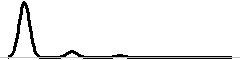
\includegraphics[width=0.8in, height=0.2in]{thesis_files/figure-latex/unnamed-chunk-1-13.png}} & \multicolumn{1}{!{\color[HTML]{000000}\vrule width 0pt}>{}c!{\color[HTML]{000000}\vrule width 0pt}}{\fontsize{11}{11}\selectfont{\textcolor[HTML]{000000}{\global\setmainfont{Latin Modern Roman}1.00}}} \\





\multicolumn{1}{!{\color[HTML]{000000}\vrule width 0pt}>{}l}{\fontsize{11}{11}\selectfont{\textcolor[HTML]{000000}{\global\setmainfont{Latin Modern Roman}}}} & \multicolumn{1}{!{\color[HTML]{000000}\vrule width 0pt}>{}l}{\fontsize{11}{11}\selectfont{\textcolor[HTML]{000000}{\global\setmainfont{Latin Modern Roman}Commercial Dest.}}} & \multicolumn{1}{!{\color[HTML]{000000}\vrule width 0pt}>{}c}{\fontsize{11}{11}\selectfont{\textcolor[HTML]{000000}{\global\setmainfont{Latin Modern Roman}0.21}}} & \multicolumn{1}{!{\color[HTML]{000000}\vrule width 0pt}>{}c}{\fontsize{11}{11}\selectfont{\textcolor[HTML]{000000}{\global\setmainfont{Latin Modern Roman}0.26}}} & \multicolumn{1}{!{\color[HTML]{000000}\vrule width 0pt}>{}c}{\fontsize{11}{11}\selectfont{\textcolor[HTML]{000000}{\global\setmainfont{Latin Modern Roman}0.00}}} & \multicolumn{1}{!{\color[HTML]{000000}\vrule width 0pt}>{}c}{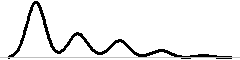
\includegraphics[width=0.8in, height=0.2in]{thesis_files/figure-latex/unnamed-chunk-1-14.png}} & \multicolumn{1}{!{\color[HTML]{000000}\vrule width 0pt}>{}c!{\color[HTML]{000000}\vrule width 0pt}}{\fontsize{11}{11}\selectfont{\textcolor[HTML]{000000}{\global\setmainfont{Latin Modern Roman}1.00}}} \\





\multicolumn{1}{!{\color[HTML]{000000}\vrule width 0pt}>{}l}{\fontsize{11}{11}\selectfont{\textcolor[HTML]{000000}{\global\setmainfont{Latin Modern Roman}}}} & \multicolumn{1}{!{\color[HTML]{000000}\vrule width 0pt}>{}l}{\fontsize{11}{11}\selectfont{\textcolor[HTML]{000000}{\global\setmainfont{Latin Modern Roman}Liquor}}} & \multicolumn{1}{!{\color[HTML]{000000}\vrule width 0pt}>{}c}{\fontsize{11}{11}\selectfont{\textcolor[HTML]{000000}{\global\setmainfont{Latin Modern Roman}0.03}}} & \multicolumn{1}{!{\color[HTML]{000000}\vrule width 0pt}>{}c}{\fontsize{11}{11}\selectfont{\textcolor[HTML]{000000}{\global\setmainfont{Latin Modern Roman}0.10}}} & \multicolumn{1}{!{\color[HTML]{000000}\vrule width 0pt}>{}c}{\fontsize{11}{11}\selectfont{\textcolor[HTML]{000000}{\global\setmainfont{Latin Modern Roman}0.00}}} & \multicolumn{1}{!{\color[HTML]{000000}\vrule width 0pt}>{}c}{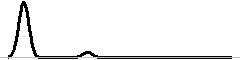
\includegraphics[width=0.8in, height=0.2in]{thesis_files/figure-latex/unnamed-chunk-1-15.png}} & \multicolumn{1}{!{\color[HTML]{000000}\vrule width 0pt}>{}c!{\color[HTML]{000000}\vrule width 0pt}}{\fontsize{11}{11}\selectfont{\textcolor[HTML]{000000}{\global\setmainfont{Latin Modern Roman}0.75}}} \\





\multicolumn{1}{!{\color[HTML]{000000}\vrule width 0pt}>{}l}{\fontsize{11}{11}\selectfont{\textcolor[HTML]{000000}{\global\setmainfont{Latin Modern Roman}}}} & \multicolumn{1}{!{\color[HTML]{000000}\vrule width 0pt}>{}l}{\fontsize{11}{11}\selectfont{\textcolor[HTML]{000000}{\global\setmainfont{Latin Modern Roman}Mixed Use}}} & \multicolumn{1}{!{\color[HTML]{000000}\vrule width 0pt}>{}c}{\fontsize{11}{11}\selectfont{\textcolor[HTML]{000000}{\global\setmainfont{Latin Modern Roman}0.32}}} & \multicolumn{1}{!{\color[HTML]{000000}\vrule width 0pt}>{}c}{\fontsize{11}{11}\selectfont{\textcolor[HTML]{000000}{\global\setmainfont{Latin Modern Roman}0.32}}} & \multicolumn{1}{!{\color[HTML]{000000}\vrule width 0pt}>{}c}{\fontsize{11}{11}\selectfont{\textcolor[HTML]{000000}{\global\setmainfont{Latin Modern Roman}0.00}}} & \multicolumn{1}{!{\color[HTML]{000000}\vrule width 0pt}>{}c}{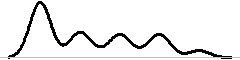
\includegraphics[width=0.8in, height=0.2in]{thesis_files/figure-latex/unnamed-chunk-1-16.png}} & \multicolumn{1}{!{\color[HTML]{000000}\vrule width 0pt}>{}c!{\color[HTML]{000000}\vrule width 0pt}}{\fontsize{11}{11}\selectfont{\textcolor[HTML]{000000}{\global\setmainfont{Latin Modern Roman}1.00}}} \\





\multicolumn{1}{!{\color[HTML]{000000}\vrule width 0pt}>{}l}{\fontsize{11}{11}\selectfont{\textcolor[HTML]{000000}{\global\setmainfont{Latin Modern Roman}}}} & \multicolumn{1}{!{\color[HTML]{000000}\vrule width 0pt}>{}l}{\fontsize{11}{11}\selectfont{\textcolor[HTML]{000000}{\global\setmainfont{Latin Modern Roman}Parking}}} & \multicolumn{1}{!{\color[HTML]{000000}\vrule width 0pt}>{}c}{\fontsize{11}{11}\selectfont{\textcolor[HTML]{000000}{\global\setmainfont{Latin Modern Roman}0.11}}} & \multicolumn{1}{!{\color[HTML]{000000}\vrule width 0pt}>{}c}{\fontsize{11}{11}\selectfont{\textcolor[HTML]{000000}{\global\setmainfont{Latin Modern Roman}0.16}}} & \multicolumn{1}{!{\color[HTML]{000000}\vrule width 0pt}>{}c}{\fontsize{11}{11}\selectfont{\textcolor[HTML]{000000}{\global\setmainfont{Latin Modern Roman}0.00}}} & \multicolumn{1}{!{\color[HTML]{000000}\vrule width 0pt}>{}c}{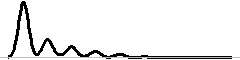
\includegraphics[width=0.8in, height=0.2in]{thesis_files/figure-latex/unnamed-chunk-1-17.png}} & \multicolumn{1}{!{\color[HTML]{000000}\vrule width 0pt}>{}c!{\color[HTML]{000000}\vrule width 0pt}}{\fontsize{11}{11}\selectfont{\textcolor[HTML]{000000}{\global\setmainfont{Latin Modern Roman}1.00}}} \\





\multicolumn{1}{!{\color[HTML]{000000}\vrule width 0pt}>{}l}{\fontsize{11}{11}\selectfont{\textcolor[HTML]{000000}{\global\setmainfont{Latin Modern Roman}}}} & \multicolumn{1}{!{\color[HTML]{000000}\vrule width 0pt}>{}l}{\fontsize{11}{11}\selectfont{\textcolor[HTML]{000000}{\global\setmainfont{Latin Modern Roman}Recreation}}} & \multicolumn{1}{!{\color[HTML]{000000}\vrule width 0pt}>{}c}{\fontsize{11}{11}\selectfont{\textcolor[HTML]{000000}{\global\setmainfont{Latin Modern Roman}0.05}}} & \multicolumn{1}{!{\color[HTML]{000000}\vrule width 0pt}>{}c}{\fontsize{11}{11}\selectfont{\textcolor[HTML]{000000}{\global\setmainfont{Latin Modern Roman}0.09}}} & \multicolumn{1}{!{\color[HTML]{000000}\vrule width 0pt}>{}c}{\fontsize{11}{11}\selectfont{\textcolor[HTML]{000000}{\global\setmainfont{Latin Modern Roman}0.00}}} & \multicolumn{1}{!{\color[HTML]{000000}\vrule width 0pt}>{}c}{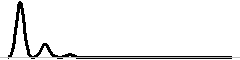
\includegraphics[width=0.8in, height=0.2in]{thesis_files/figure-latex/unnamed-chunk-1-18.png}} & \multicolumn{1}{!{\color[HTML]{000000}\vrule width 0pt}>{}c!{\color[HTML]{000000}\vrule width 0pt}}{\fontsize{11}{11}\selectfont{\textcolor[HTML]{000000}{\global\setmainfont{Latin Modern Roman}1.00}}} \\





\multicolumn{1}{!{\color[HTML]{000000}\vrule width 0pt}>{}l}{\fontsize{11}{11}\selectfont{\textcolor[HTML]{000000}{\global\setmainfont{Latin Modern Roman}}}} & \multicolumn{1}{!{\color[HTML]{000000}\vrule width 0pt}>{}l}{\fontsize{11}{11}\selectfont{\textcolor[HTML]{000000}{\global\setmainfont{Latin Modern Roman}Vacant}}} & \multicolumn{1}{!{\color[HTML]{000000}\vrule width 0pt}>{}c}{\fontsize{11}{11}\selectfont{\textcolor[HTML]{000000}{\global\setmainfont{Latin Modern Roman}0.12}}} & \multicolumn{1}{!{\color[HTML]{000000}\vrule width 0pt}>{}c}{\fontsize{11}{11}\selectfont{\textcolor[HTML]{000000}{\global\setmainfont{Latin Modern Roman}0.21}}} & \multicolumn{1}{!{\color[HTML]{000000}\vrule width 0pt}>{}c}{\fontsize{11}{11}\selectfont{\textcolor[HTML]{000000}{\global\setmainfont{Latin Modern Roman}0.00}}} & \multicolumn{1}{!{\color[HTML]{000000}\vrule width 0pt}>{}c}{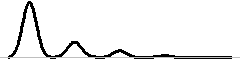
\includegraphics[width=0.8in, height=0.2in]{thesis_files/figure-latex/unnamed-chunk-1-19.png}} & \multicolumn{1}{!{\color[HTML]{000000}\vrule width 0pt}>{}c!{\color[HTML]{000000}\vrule width 0pt}}{\fontsize{11}{11}\selectfont{\textcolor[HTML]{000000}{\global\setmainfont{Latin Modern Roman}1.00}}} \\





\multicolumn{1}{!{\color[HTML]{000000}\vrule width 0pt}>{}l}{\fontsize{11}{11}\selectfont{\textcolor[HTML]{000000}{\global\setmainfont{Latin Modern Roman}}}} & \multicolumn{1}{!{\color[HTML]{000000}\vrule width 0pt}>{}l}{\fontsize{11}{11}\selectfont{\textcolor[HTML]{000000}{\global\setmainfont{Latin Modern Roman}Density (Block)}}} & \multicolumn{1}{!{\color[HTML]{000000}\vrule width 0pt}>{}c}{\fontsize{11}{11}\selectfont{\textcolor[HTML]{000000}{\global\setmainfont{Latin Modern Roman}10.85}}} & \multicolumn{1}{!{\color[HTML]{000000}\vrule width 0pt}>{}c}{\fontsize{11}{11}\selectfont{\textcolor[HTML]{000000}{\global\setmainfont{Latin Modern Roman}7.59}}} & \multicolumn{1}{!{\color[HTML]{000000}\vrule width 0pt}>{}c}{\fontsize{11}{11}\selectfont{\textcolor[HTML]{000000}{\global\setmainfont{Latin Modern Roman}0.00}}} & \multicolumn{1}{!{\color[HTML]{000000}\vrule width 0pt}>{}c}{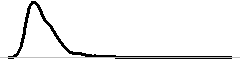
\includegraphics[width=0.8in, height=0.2in]{thesis_files/figure-latex/unnamed-chunk-1-20.png}} & \multicolumn{1}{!{\color[HTML]{000000}\vrule width 0pt}>{}c!{\color[HTML]{000000}\vrule width 0pt}}{\fontsize{11}{11}\selectfont{\textcolor[HTML]{000000}{\global\setmainfont{Latin Modern Roman}83.42}}} \\

\noalign{\global\setlength{\arrayrulewidth}{1pt}}\arrayrulecolor[HTML]{000000}\cline{1-7}

\end{longtable}
\hypertarget{methods}{%
\section{Methods}\label{methods}}

I examine the relationships between collective efficacy, the built environment, and crime using a system of piecewise structural equations (see: Figure \ref{fig:longmodels}) which consist of (1) negative binomial mixed models of conditional direct associations of collective efficacy and built environment characteristics with crime and, (2) linear mixed models predicting present collective efficacy and built environment conditions using past collective efficacy. Piecewise structural equations are an alternative to conventional variance-covariance based structural equation models (SEM) which instead decompose the structural model into component regressions estimated separately (Shipley 2016). This permits use of estimators which are unsupported in conventional SEM software or are computationally intractable. In the present case, a piecewise approach permits mixing single- and multi-level linear and negative binomial (gamma-poisson) models.

Because the component models are estimated individually, the fit of a piecewise system of equations is evaluated using tests of directed separation (d-separation) for each independence restriction in the system of models. In this case, the tests of direct separations are based on the significance of correlations between the residuals of endogenous variables and/or observed values of exogenous variables which the structural model implies should be zero (Shipley 2016). These d-separation tests may then be summarized by a single Fisher's C statistic which measures overall fit similar to chi-square tests based on comparisons of observed and predicted covariance matrices in conventional SEM. Both the Fisher's C statistic and SEM chi-square may be described as simultaneous tests of the validity of all restrictions implied by the structural models.
\begin{figure}

\includegraphics[width=1\linewidth]{./figure/ch2/longitudinal_models} \caption{Longitudinal  structural model. Dashed arrow represents tested independence restriction (d-separation).}\label{fig:longmodels}
\end{figure}
Figure \ref{fig:longmodels} is a simplified version of the complete structural model. Each solid arrow represents separate model or set of models testing the hypothesized causal pathways. The dashed arrow from past collective efficacy to crime is expected to be zero conditional on the included measures. This is evaluated using a test of d-separation for each outcome. The entire system of models was estimated together using the R package \texttt{piecewiseSEM} (Lefcheck 2016; R Core Team 2021).

All models---whether predicting crime or built environment conditions---adjust for neighborhood disadvantage, stability, and Hispanic/immigrant population. These models also adjust for neighborhood-level and block-level population density, rather than using a population offset to directly model rates as is often advised in models of crime counts (Osgood 2000). This choice was made because it is unlikely block-level populations capture only the number of individuals at risk in a given block. Population density instead is likely to capture variation in all three key elements of criminal opportunity---likely offenders, suitable targets, and capable guardians---which is unaccounted for by the other structural covariates. Testing different functional forms of density revealed a strong quadratic relationship at the block-level in all models, which might be expected if density captures both potential targets and guardians: Crime is more likely to occur where there are sufficient people present to make targets abundant but not so many as to make it likely the crime will be observed or interrupted (e.g., St. Jean 2007:156). Inclusion of the density measures is also conservative, as removing them strengthens, rather than weakens the focal relationships.

While the models below take steps to address residual correlations---such as neighborhood random intercepts---I do not model spatial dependence between observations as is sometimes done in this literature (e.g., Morenoff, Sampson, and Raudenbush 2001). This choice was made because the units of observation are from a sample of only 1,641 out of Chicago's 20,000-some census-blocks. Most sampled blocks are not adjacent to another sampled block (see Figure \ref{fig:blocksample} above). This which prevents calculating adjacency-based spatial weights for spatial regression models or conducting tests of spatial dependence based on neighbor matrices (such as Moran's I).

\hypertarget{models-of-crime}{%
\subsection{Models of Crime}\label{models-of-crime}}

Hypothesis 1 proposes there is a conditional direct association between built environment features and specific types of crime based on the form of opportunities they provide---for instance, I expect commercial destinations to better predict robbery and property crime than homicide and gun assaults. While commercial destinations may promote crime of all kinds by bringing many people together, commercial destinations in particular feature suitable targets for theft (merchandise) and robbery (customers carrying cash). Figure \ref{fig:directmodels} is a simplified diagram of the model focusing on the measures of interest. Note that the built environment box represents all eight built environment features---bars, liquor stores, vacant lots, abandoned buildings, commercial destinations, recreation facilities, parking lots, and mixed land use---and crime represents all five crime types---homicide, gun assaults, robbery, any violent crime, and any property crime. In all cases I expect a direct effect of collective efficacy on crime due to the mechanism of informal social control (and other forms of intervention). The dotted line indicates unmodeled pathways which are evaluated using tests of d-separation.
\begin{figure}
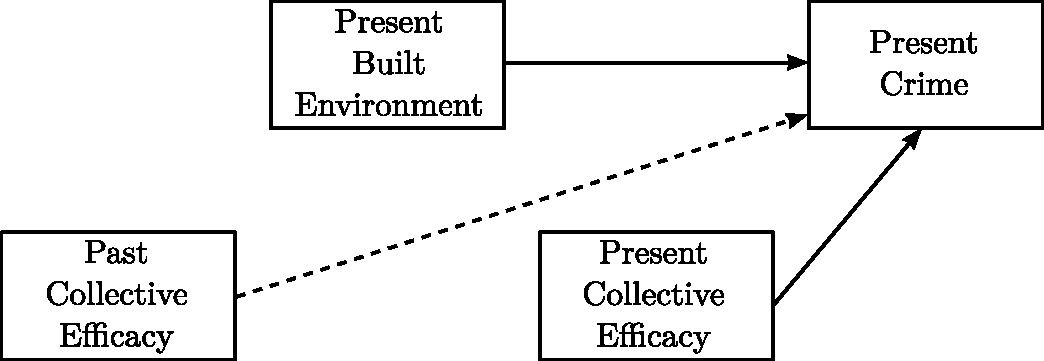
\includegraphics[width=1\linewidth]{./figure/ch2/direct_models} \caption{Simplified depiction of crime models. Solid arrows are modeled direct effects. The dashed arrow represents unmodeled (restricted) paths.}\label{fig:directmodels}
\end{figure}
I estimate the conditional direct effects of collective efficacy and the built environment on crime using negative binomial models with random intercepts for neighborhood clusters fit using R's \texttt{lme4} package (Bates et al. 2015). Cluster intercepts address correlations in residuals for blocks in the same neighborhood. Conditional on the included covariates, the intra-class correlations are modest (between 0.10 and 0.20 depending on crime type), however BIC values and likelihood ratio tests indicate specifications with the random effects are at least weakly preferred except for homicide. In the case of homicide, the random effects do not improve model fit and cannot be stably estimated. Consequently, homicide is estimated with a conventional pooled negative binomial model which produces point estimates for the parameters of interest that are indistinguishable from those of the multilevel model.

\hypertarget{models-of-the-built-environment-and-present-collective-efficacy}{%
\subsection{Models of the Built Environment and Present Collective Efficacy}\label{models-of-the-built-environment-and-present-collective-efficacy}}

The next set of models estimate the conditional direct associations between past collective and the built environment, and between both past collective efficacy and the built environment and present collective efficacy. Hypothesis 2 posits that past collective influences the built environment, and Hypothesis 3 posits that features of the built environment impact collective efficacy. The solid arrows in Figure \ref{fig:cebemodel} depict the tested relationships.
\begin{figure}

{\centering 
\includegraphics[width=0.75\linewidth]{./figure/ch2/ce_be_model} 

}

\caption{Models of the built environment and present collective efficacy.}\label{fig:cebemodel}
\end{figure}
This part of the piecewise structural model consists of pooled and multilevel linear regressions. A pooled (neighborhood-level) linear regression was used to test the paths from the built environment and past collective efficacy to present collective efficacy. Multilevel (block-in-neighborhood) linear regressions test the paths from past collective efficacy to the built environment features. As before, all models adjust for neighborhood structural characteristics, and the built environment features are permitted to correlate with each other. Note that the neighborhood structural characteristics were measured in the year 2000 and past collective efficacy was measured in 1995. If collective efficacy influences any built environment features via these structural characteristics, this amounts to controlling for a post-treatment confounder (a mediator). Consequently, this may yield conservative estimates of the relationships between past collective efficacy and both the built environment and present collective efficacy.

\hypertarget{results}{%
\section{Results}\label{results}}

This section presents results from each set of models described above. The first subsection, Crime Results, provides estimates for the conditional direct associations of collective efficacy, the built environment, and tract- and block-level control with the five forms of police-reported crime. The second subsection, Built Environment and Collective Efficacy Results, contains estimates of the associations between past collective efficacy and the built environment, and the built environment and present collective efficacy.

\hypertarget{crime-results}{%
\subsection{Crime Results}\label{crime-results}}

Figure \ref{fig:coefplot} displays incidence rate ratios (IRR) for the conditional direct associations between the primary predictors of interest---collective efficacy and the built environment features---and crime. Each column represents a model for a different crime type. The displayed IRR is the estimated multiplicative difference in the count of crime incidents of a given type for a one standard deviation difference in the predictor. For example, a one standard deviation higher level of in abandoned buildings---21\% more block faces with abandoned buildings on and around that block---is expected to be associated with, on average, about 20\% more homicides and gun assaults than otherwise similar block.
\begin{figure}

{\centering 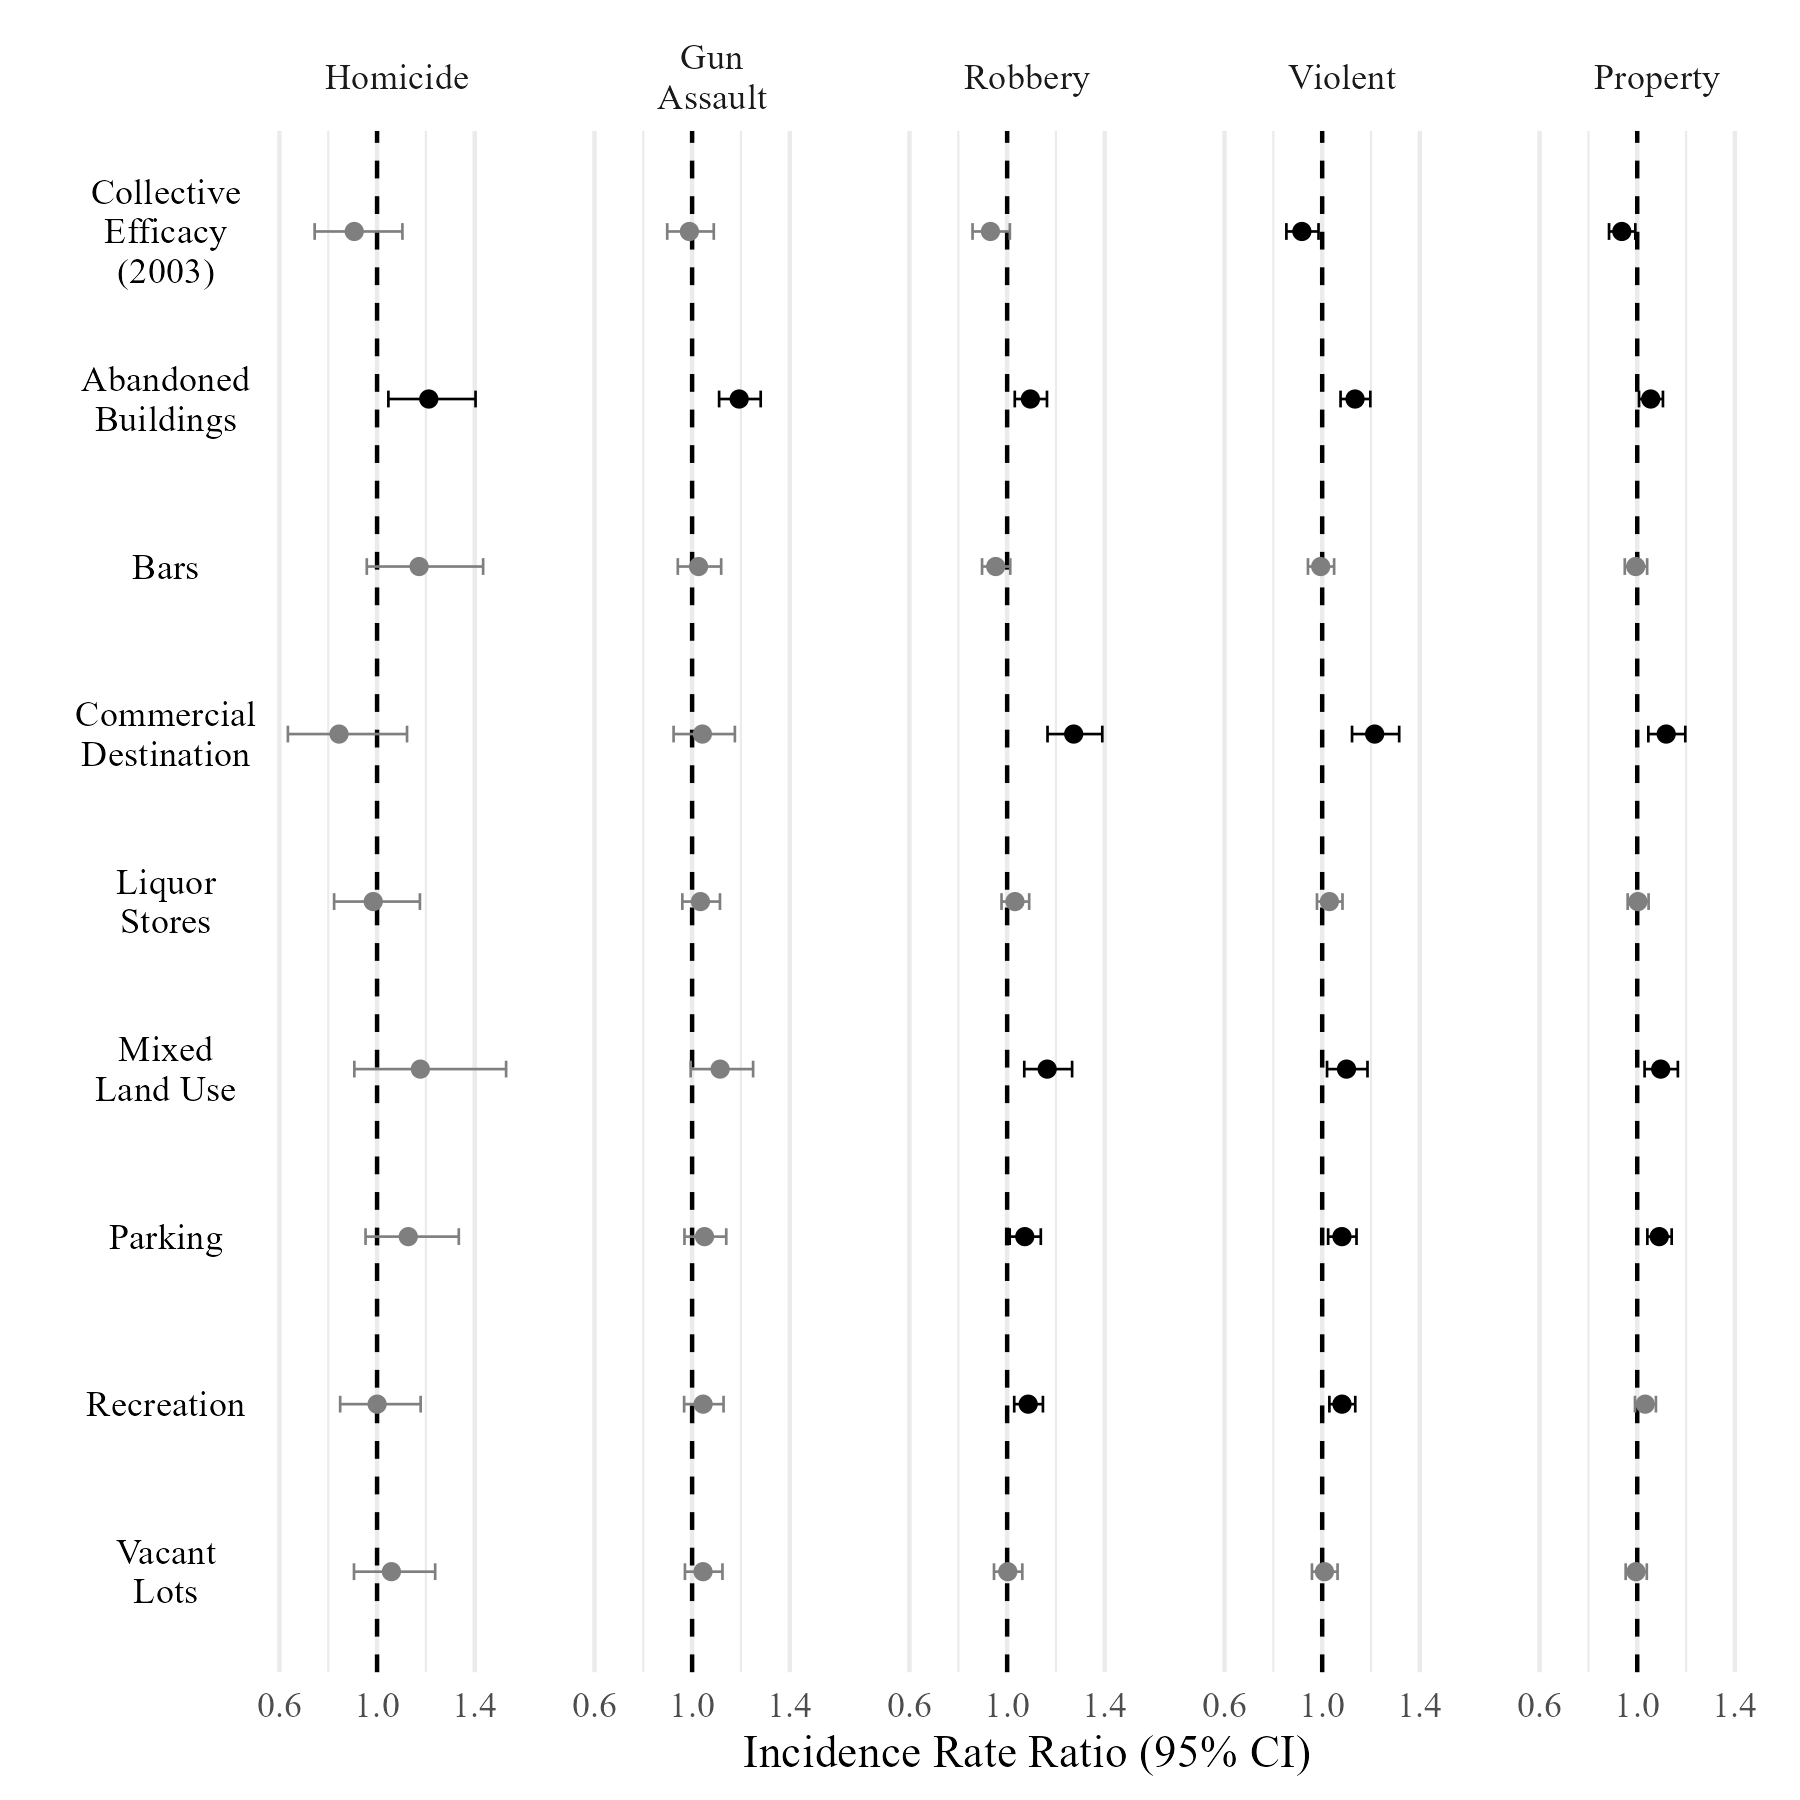
\includegraphics[width=1\linewidth]{./figure/ch2/coefplot_stage_2} 

}

\caption{Estimated incidence rate ratios and 95\% confidence intervals for selected predictors of five crime types. Predictors are standardized, outcomes are log-counts. Estimates significant at $p < .05$ are in black.}\label{fig:coefplot}
\end{figure}
The most notable result in Figure \ref{fig:coefplot} is the weak conditional direct association between collective efficacy and the five crime outcomes. Estimated IRRs for collective efficacy are between 0.91 and 0.94 across all outcomes except gun assault (0.99). Statistical significance of collective efficacy for the violence and property crime outcomes is a function of their higher frequency, and thus greater statistical power to detect effects, rather than of stronger relationships. These weak associations are not, however, the result of inclusion of the built environment features. Removing these features produces only slightly stronger estimates for collective efficacy. Overall, collective efficacy appears to have a modest relationship with crime in these data.

In contrast, the conditional direct associations of built environment features with crime are comparatively large as proposed in Hypothesis 1. Homicide and gun assaults are significantly predicted only by abandoned buildings. All violent crimes, robbery, and property crimes are also associated with abandoned buildings, though less so. Features which provide targets of monetary value---commercial destinations, mixed land use, parking---are more strongly associated with robbery and property crime than homicide and gun assault. These features do, however, show similar associations with all violent crime. As noted before, this may be expected if these built environment features are associated with increased foot traffic, which increases the potential for interpersonal interactions of any kind, including violent ones.

Against Hypothesis 1, vacant lots, bars, and liquors stores show no notable relationship with crime, and no features other than abandoned buildings exhibit a statistically significant association with homicide and gun violence. With regard to vacant lots, bars, and liquor stores, the absence of the expected associations may be due to treatment heterogeneity: The measures used do not distinguish between different types of establishments or vacant lots. It is possible, for example, that abandoned buildings are nearly always suitable for concealing weapons but only particular vacant lots are suitable---such as those with substantial debris or foliage. Similarly, it is likely certain bars provoke violence---due to service practices, property management, or clientele---while others do not, or even reduce it through monitoring and reporting of problems (Graham et al. 2006). The present research design is unable to examine potential heterogeneity of this sort. Appendix \ref{bemoderation} examines the possibility that the effects of built environment features are moderated by collective efficacy---which might capture some heterogeneity---but I find little evidence for this.

For reference, the full model estimates, including controls, are found in Table \ref{tab:secondstage} below. These estimates are the log-count marginal effects on crime from one standard deviation differences in predictors. \(R^{2}\) is Nagelkerke for homicide (single-level model) and marginal Trigamma for the other outcomes. That is, the value of 0.56 for the Disadvantage row in the Homicide column indicates a one standard deviation higher level of disadvantage is associated with a 0.56 higher log-count of homicides on a given block. The IRR estimates in Figure @ref\{fig:coefplot\} are exponentiated values of these same estimates. The non-significant d-separation test p-values at the bottom of the table also indicate no association was found between past collective efficacy and any of the crime outcomes net of included tract and block covariates (Overall Fisher's \(C = 9.99\), \(df = 10\), \(p = 0.44\)). This result is consistent with the expectation, shown as a dashed line in Figure \ref{fig:directmodels}, that past collective efficacy exerts no protective effect on crime except via present collective efficacy or the built environment.

\clearpage
\providecommand{\docline}[3]{\noalign{\global\setlength{\arrayrulewidth}{#1}}\arrayrulecolor[HTML]{#2}\cline{#3}}

\setlength{\tabcolsep}{4pt}

\renewcommand*{\arraystretch}{0.65}
\begin{longtable}[c]{|p{0.10in}|p{0.80in}|p{0.75in}|p{0.75in}|p{0.75in}|p{0.75in}|p{0.75in}}

\caption{\label{tab:secondstage} Negative Binomial Estimates of Crime}\label{tab:unnamed-chunk-2}\\

\hhline{>{\arrayrulecolor[HTML]{000000}\global\arrayrulewidth=1pt}->{\arrayrulecolor[HTML]{000000}\global\arrayrulewidth=1pt}->{\arrayrulecolor[HTML]{000000}\global\arrayrulewidth=1pt}->{\arrayrulecolor[HTML]{000000}\global\arrayrulewidth=1pt}->{\arrayrulecolor[HTML]{000000}\global\arrayrulewidth=1pt}->{\arrayrulecolor[HTML]{000000}\global\arrayrulewidth=1pt}->{\arrayrulecolor[HTML]{000000}\global\arrayrulewidth=1pt}-}

\multicolumn{1}{!{\color[HTML]{000000}\vrule width 0pt}>{\raggedright}p{\dimexpr 0.1in+0\tabcolsep+0\arrayrulewidth}}{\fontsize{10}{10}\selectfont{\textcolor[HTML]{000000}{\global\setmainfont{Latin Modern Roman}}}} & \multicolumn{1}{!{\color[HTML]{000000}\vrule width 0pt}>{\raggedright}p{\dimexpr 0.8in+0\tabcolsep+0\arrayrulewidth}}{\fontsize{10}{10}\selectfont{\textcolor[HTML]{000000}{\global\setmainfont{Latin Modern Roman}Predictor}}} & \multicolumn{1}{!{\color[HTML]{000000}\vrule width 0pt}>{\centering}p{\dimexpr 0.75in+0\tabcolsep+0\arrayrulewidth}}{\fontsize{10}{10}\selectfont{\textcolor[HTML]{000000}{\global\setmainfont{Latin Modern Roman}Homicide}}} & \multicolumn{1}{!{\color[HTML]{000000}\vrule width 0pt}>{\centering}p{\dimexpr 0.75in+0\tabcolsep+0\arrayrulewidth}}{\fontsize{10}{10}\selectfont{\textcolor[HTML]{000000}{\global\setmainfont{Latin Modern Roman}Gun Assault}}} & \multicolumn{1}{!{\color[HTML]{000000}\vrule width 0pt}>{\centering}p{\dimexpr 0.75in+0\tabcolsep+0\arrayrulewidth}}{\fontsize{10}{10}\selectfont{\textcolor[HTML]{000000}{\global\setmainfont{Latin Modern Roman}Robbery}}} & \multicolumn{1}{!{\color[HTML]{000000}\vrule width 0pt}>{\centering}p{\dimexpr 0.75in+0\tabcolsep+0\arrayrulewidth}}{\fontsize{10}{10}\selectfont{\textcolor[HTML]{000000}{\global\setmainfont{Latin Modern Roman}Violent}}} & \multicolumn{1}{!{\color[HTML]{000000}\vrule width 0pt}>{\centering}p{\dimexpr 0.75in+0\tabcolsep+0\arrayrulewidth}!{\color[HTML]{000000}\vrule width 0pt}}{\fontsize{10}{10}\selectfont{\textcolor[HTML]{000000}{\global\setmainfont{Latin Modern Roman}Property}}} \\

\noalign{\global\setlength{\arrayrulewidth}{0.5pt}}\arrayrulecolor[HTML]{000000}\cline{1-7}

\endfirsthead

\hhline{>{\arrayrulecolor[HTML]{000000}\global\arrayrulewidth=1pt}->{\arrayrulecolor[HTML]{000000}\global\arrayrulewidth=1pt}->{\arrayrulecolor[HTML]{000000}\global\arrayrulewidth=1pt}->{\arrayrulecolor[HTML]{000000}\global\arrayrulewidth=1pt}->{\arrayrulecolor[HTML]{000000}\global\arrayrulewidth=1pt}->{\arrayrulecolor[HTML]{000000}\global\arrayrulewidth=1pt}->{\arrayrulecolor[HTML]{000000}\global\arrayrulewidth=1pt}-}

\multicolumn{1}{!{\color[HTML]{000000}\vrule width 0pt}>{\raggedright}p{\dimexpr 0.1in+0\tabcolsep+0\arrayrulewidth}}{\fontsize{10}{10}\selectfont{\textcolor[HTML]{000000}{\global\setmainfont{Latin Modern Roman}}}} & \multicolumn{1}{!{\color[HTML]{000000}\vrule width 0pt}>{\raggedright}p{\dimexpr 0.8in+0\tabcolsep+0\arrayrulewidth}}{\fontsize{10}{10}\selectfont{\textcolor[HTML]{000000}{\global\setmainfont{Latin Modern Roman}Predictor}}} & \multicolumn{1}{!{\color[HTML]{000000}\vrule width 0pt}>{\centering}p{\dimexpr 0.75in+0\tabcolsep+0\arrayrulewidth}}{\fontsize{10}{10}\selectfont{\textcolor[HTML]{000000}{\global\setmainfont{Latin Modern Roman}Homicide}}} & \multicolumn{1}{!{\color[HTML]{000000}\vrule width 0pt}>{\centering}p{\dimexpr 0.75in+0\tabcolsep+0\arrayrulewidth}}{\fontsize{10}{10}\selectfont{\textcolor[HTML]{000000}{\global\setmainfont{Latin Modern Roman}Gun Assault}}} & \multicolumn{1}{!{\color[HTML]{000000}\vrule width 0pt}>{\centering}p{\dimexpr 0.75in+0\tabcolsep+0\arrayrulewidth}}{\fontsize{10}{10}\selectfont{\textcolor[HTML]{000000}{\global\setmainfont{Latin Modern Roman}Robbery}}} & \multicolumn{1}{!{\color[HTML]{000000}\vrule width 0pt}>{\centering}p{\dimexpr 0.75in+0\tabcolsep+0\arrayrulewidth}}{\fontsize{10}{10}\selectfont{\textcolor[HTML]{000000}{\global\setmainfont{Latin Modern Roman}Violent}}} & \multicolumn{1}{!{\color[HTML]{000000}\vrule width 0pt}>{\centering}p{\dimexpr 0.75in+0\tabcolsep+0\arrayrulewidth}!{\color[HTML]{000000}\vrule width 0pt}}{\fontsize{10}{10}\selectfont{\textcolor[HTML]{000000}{\global\setmainfont{Latin Modern Roman}Property}}} \\

\noalign{\global\setlength{\arrayrulewidth}{0.5pt}}\arrayrulecolor[HTML]{000000}\cline{1-7}\endhead



\multicolumn{2}{!{\color[HTML]{000000}\vrule width 0pt}>{\raggedright}p{\dimexpr 0.9in+2\tabcolsep+1\arrayrulewidth}}{\fontsize{10}{10}\selectfont{\textcolor[HTML]{000000}{\global\setmainfont{Latin Modern Roman}Past Coll. Eff.\linebreak d-Sep. P-value}}} & \multicolumn{1}{!{\color[HTML]{000000}\vrule width 0pt}>{\centering}p{\dimexpr 0.75in+0\tabcolsep+0\arrayrulewidth}}{\fontsize{10}{10}\selectfont{\textcolor[HTML]{000000}{\global\setmainfont{Latin Modern Roman}0.48}}} & \multicolumn{1}{!{\color[HTML]{000000}\vrule width 0pt}>{\centering}p{\dimexpr 0.75in+0\tabcolsep+0\arrayrulewidth}}{\fontsize{10}{10}\selectfont{\textcolor[HTML]{000000}{\global\setmainfont{Latin Modern Roman}0.23}}} & \multicolumn{1}{!{\color[HTML]{000000}\vrule width 0pt}>{\centering}p{\dimexpr 0.75in+0\tabcolsep+0\arrayrulewidth}}{\fontsize{10}{10}\selectfont{\textcolor[HTML]{000000}{\global\setmainfont{Latin Modern Roman}0.92}}} & \multicolumn{1}{!{\color[HTML]{000000}\vrule width 0pt}>{\centering}p{\dimexpr 0.75in+0\tabcolsep+0\arrayrulewidth}}{\fontsize{10}{10}\selectfont{\textcolor[HTML]{000000}{\global\setmainfont{Latin Modern Roman}0.13}}} & \multicolumn{1}{!{\color[HTML]{000000}\vrule width 0pt}>{\centering}p{\dimexpr 0.75in+0\tabcolsep+0\arrayrulewidth}!{\color[HTML]{000000}\vrule width 0pt}}{\fontsize{10}{10}\selectfont{\textcolor[HTML]{000000}{\global\setmainfont{Latin Modern Roman}0.52}}} \\





\multicolumn{2}{!{\color[HTML]{000000}\vrule width 0pt}>{\raggedright}p{\dimexpr 0.9in+2\tabcolsep+1\arrayrulewidth}}{\fontsize{10}{10}\selectfont{\textcolor[HTML]{000000}{\global\setmainfont{Latin Modern Roman}R2}}} & \multicolumn{1}{!{\color[HTML]{000000}\vrule width 0pt}>{\centering}p{\dimexpr 0.75in+0\tabcolsep+0\arrayrulewidth}}{\fontsize{10}{10}\selectfont{\textcolor[HTML]{000000}{\global\setmainfont{Latin Modern Roman}0.14}}} & \multicolumn{1}{!{\color[HTML]{000000}\vrule width 0pt}>{\centering}p{\dimexpr 0.75in+0\tabcolsep+0\arrayrulewidth}}{\fontsize{10}{10}\selectfont{\textcolor[HTML]{000000}{\global\setmainfont{Latin Modern Roman}0.17}}} & \multicolumn{1}{!{\color[HTML]{000000}\vrule width 0pt}>{\centering}p{\dimexpr 0.75in+0\tabcolsep+0\arrayrulewidth}}{\fontsize{10}{10}\selectfont{\textcolor[HTML]{000000}{\global\setmainfont{Latin Modern Roman}0.28}}} & \multicolumn{1}{!{\color[HTML]{000000}\vrule width 0pt}>{\centering}p{\dimexpr 0.75in+0\tabcolsep+0\arrayrulewidth}}{\fontsize{10}{10}\selectfont{\textcolor[HTML]{000000}{\global\setmainfont{Latin Modern Roman}0.36}}} & \multicolumn{1}{!{\color[HTML]{000000}\vrule width 0pt}>{\centering}p{\dimexpr 0.75in+0\tabcolsep+0\arrayrulewidth}!{\color[HTML]{000000}\vrule width 0pt}}{\fontsize{10}{10}\selectfont{\textcolor[HTML]{000000}{\global\setmainfont{Latin Modern Roman}0.29}}} \\

\noalign{\global\setlength{\arrayrulewidth}{1pt}}\arrayrulecolor[HTML]{000000}\cline{1-7}\endfoot



\multicolumn{7}{!{\color[HTML]{000000}\vrule width 0pt}>{\raggedright}p{\dimexpr 4.65in+12\tabcolsep+6\arrayrulewidth}}{\fontsize{10}{10}\selectfont{\textcolor[HTML]{000000}{\global\setmainfont{Latin Modern Roman}\textit{Neighborhood}}}} \\





\multicolumn{1}{!{\color[HTML]{000000}\vrule width 0pt}>{\raggedright}p{\dimexpr 0.1in+0\tabcolsep+0\arrayrulewidth}}{\fontsize{10}{10}\selectfont{\textcolor[HTML]{000000}{\global\setmainfont{Latin Modern Roman}}}} & \multicolumn{1}{!{\color[HTML]{000000}\vrule width 0pt}>{\raggedright}p{\dimexpr 0.8in+0\tabcolsep+0\arrayrulewidth}}{\fontsize{10}{10}\selectfont{\textcolor[HTML]{000000}{\global\setmainfont{Latin Modern Roman}Coll. Eff (2001)}}} & \multicolumn{1}{!{\color[HTML]{000000}\vrule width 0pt}>{\centering}p{\dimexpr 0.75in+0\tabcolsep+0\arrayrulewidth}}{\fontsize{10}{10}\selectfont{\textcolor[HTML]{000000}{\global\setmainfont{Latin Modern Roman}-0.10}}\fontsize{10}{10}\selectfont{\textcolor[HTML]{000000}{\global\setmainfont{Latin Modern Roman}\linebreak }}\fontsize{10}{10}\selectfont{\textcolor[HTML]{000000}{\global\setmainfont{Latin Modern Roman}(}}\fontsize{10}{10}\selectfont{\textcolor[HTML]{000000}{\global\setmainfont{Latin Modern Roman}0.10}}\fontsize{10}{10}\selectfont{\textcolor[HTML]{000000}{\global\setmainfont{Latin Modern Roman})}}} & \multicolumn{1}{!{\color[HTML]{000000}\vrule width 0pt}>{\centering}p{\dimexpr 0.75in+0\tabcolsep+0\arrayrulewidth}}{\fontsize{10}{10}\selectfont{\textcolor[HTML]{000000}{\global\setmainfont{Latin Modern Roman}-0.01}}\fontsize{10}{10}\selectfont{\textcolor[HTML]{000000}{\global\setmainfont{Latin Modern Roman}\linebreak }}\fontsize{10}{10}\selectfont{\textcolor[HTML]{000000}{\global\setmainfont{Latin Modern Roman}(}}\fontsize{10}{10}\selectfont{\textcolor[HTML]{000000}{\global\setmainfont{Latin Modern Roman}0.05}}\fontsize{10}{10}\selectfont{\textcolor[HTML]{000000}{\global\setmainfont{Latin Modern Roman})}}} & \multicolumn{1}{!{\color[HTML]{000000}\vrule width 0pt}>{\centering}p{\dimexpr 0.75in+0\tabcolsep+0\arrayrulewidth}}{\fontsize{10}{10}\selectfont{\textcolor[HTML]{000000}{\global\setmainfont{Latin Modern Roman}-0.07}}\fontsize{10}{10}\selectfont{\textcolor[HTML]{000000}{\global\setmainfont{Latin Modern Roman}\linebreak }}\fontsize{10}{10}\selectfont{\textcolor[HTML]{000000}{\global\setmainfont{Latin Modern Roman}(}}\fontsize{10}{10}\selectfont{\textcolor[HTML]{000000}{\global\setmainfont{Latin Modern Roman}0.04}}\fontsize{10}{10}\selectfont{\textcolor[HTML]{000000}{\global\setmainfont{Latin Modern Roman})}}} & \multicolumn{1}{!{\color[HTML]{000000}\vrule width 0pt}>{\centering}p{\dimexpr 0.75in+0\tabcolsep+0\arrayrulewidth}}{\fontsize{10}{10}\selectfont{\textcolor[HTML]{000000}{\global\setmainfont{Latin Modern Roman}\textbf{-0.09}}}\fontsize{10}{10}\selectfont{\textcolor[HTML]{000000}{\global\setmainfont{Latin Modern Roman}\textbf{\linebreak }}}\fontsize{10}{10}\selectfont{\textcolor[HTML]{000000}{\global\setmainfont{Latin Modern Roman}\textbf{(}}}\fontsize{10}{10}\selectfont{\textcolor[HTML]{000000}{\global\setmainfont{Latin Modern Roman}\textbf{0.04}}}\fontsize{10}{10}\selectfont{\textcolor[HTML]{000000}{\global\setmainfont{Latin Modern Roman}\textbf{)}}}} & \multicolumn{1}{!{\color[HTML]{000000}\vrule width 0pt}>{\centering}p{\dimexpr 0.75in+0\tabcolsep+0\arrayrulewidth}!{\color[HTML]{000000}\vrule width 0pt}}{\fontsize{10}{10}\selectfont{\textcolor[HTML]{000000}{\global\setmainfont{Latin Modern Roman}\textbf{-0.07}}}\fontsize{10}{10}\selectfont{\textcolor[HTML]{000000}{\global\setmainfont{Latin Modern Roman}\textbf{\linebreak }}}\fontsize{10}{10}\selectfont{\textcolor[HTML]{000000}{\global\setmainfont{Latin Modern Roman}\textbf{(}}}\fontsize{10}{10}\selectfont{\textcolor[HTML]{000000}{\global\setmainfont{Latin Modern Roman}\textbf{0.03}}}\fontsize{10}{10}\selectfont{\textcolor[HTML]{000000}{\global\setmainfont{Latin Modern Roman}\textbf{)}}}} \\





\multicolumn{1}{!{\color[HTML]{000000}\vrule width 0pt}>{\raggedright}p{\dimexpr 0.1in+0\tabcolsep+0\arrayrulewidth}}{\fontsize{10}{10}\selectfont{\textcolor[HTML]{000000}{\global\setmainfont{Latin Modern Roman}}}} & \multicolumn{1}{!{\color[HTML]{000000}\vrule width 0pt}>{\raggedright}p{\dimexpr 0.8in+0\tabcolsep+0\arrayrulewidth}}{\fontsize{10}{10}\selectfont{\textcolor[HTML]{000000}{\global\setmainfont{Latin Modern Roman}Disadv.}}} & \multicolumn{1}{!{\color[HTML]{000000}\vrule width 0pt}>{\centering}p{\dimexpr 0.75in+0\tabcolsep+0\arrayrulewidth}}{\fontsize{10}{10}\selectfont{\textcolor[HTML]{000000}{\global\setmainfont{Latin Modern Roman}\textbf{0.56}}}\fontsize{10}{10}\selectfont{\textcolor[HTML]{000000}{\global\setmainfont{Latin Modern Roman}\textbf{\linebreak }}}\fontsize{10}{10}\selectfont{\textcolor[HTML]{000000}{\global\setmainfont{Latin Modern Roman}\textbf{(}}}\fontsize{10}{10}\selectfont{\textcolor[HTML]{000000}{\global\setmainfont{Latin Modern Roman}\textbf{0.11}}}\fontsize{10}{10}\selectfont{\textcolor[HTML]{000000}{\global\setmainfont{Latin Modern Roman}\textbf{)}}}} & \multicolumn{1}{!{\color[HTML]{000000}\vrule width 0pt}>{\centering}p{\dimexpr 0.75in+0\tabcolsep+0\arrayrulewidth}}{\fontsize{10}{10}\selectfont{\textcolor[HTML]{000000}{\global\setmainfont{Latin Modern Roman}\textbf{0.70}}}\fontsize{10}{10}\selectfont{\textcolor[HTML]{000000}{\global\setmainfont{Latin Modern Roman}\textbf{\linebreak }}}\fontsize{10}{10}\selectfont{\textcolor[HTML]{000000}{\global\setmainfont{Latin Modern Roman}\textbf{(}}}\fontsize{10}{10}\selectfont{\textcolor[HTML]{000000}{\global\setmainfont{Latin Modern Roman}\textbf{0.06}}}\fontsize{10}{10}\selectfont{\textcolor[HTML]{000000}{\global\setmainfont{Latin Modern Roman}\textbf{)}}}} & \multicolumn{1}{!{\color[HTML]{000000}\vrule width 0pt}>{\centering}p{\dimexpr 0.75in+0\tabcolsep+0\arrayrulewidth}}{\fontsize{10}{10}\selectfont{\textcolor[HTML]{000000}{\global\setmainfont{Latin Modern Roman}\textbf{0.22}}}\fontsize{10}{10}\selectfont{\textcolor[HTML]{000000}{\global\setmainfont{Latin Modern Roman}\textbf{\linebreak }}}\fontsize{10}{10}\selectfont{\textcolor[HTML]{000000}{\global\setmainfont{Latin Modern Roman}\textbf{(}}}\fontsize{10}{10}\selectfont{\textcolor[HTML]{000000}{\global\setmainfont{Latin Modern Roman}\textbf{0.04}}}\fontsize{10}{10}\selectfont{\textcolor[HTML]{000000}{\global\setmainfont{Latin Modern Roman}\textbf{)}}}} & \multicolumn{1}{!{\color[HTML]{000000}\vrule width 0pt}>{\centering}p{\dimexpr 0.75in+0\tabcolsep+0\arrayrulewidth}}{\fontsize{10}{10}\selectfont{\textcolor[HTML]{000000}{\global\setmainfont{Latin Modern Roman}\textbf{0.39}}}\fontsize{10}{10}\selectfont{\textcolor[HTML]{000000}{\global\setmainfont{Latin Modern Roman}\textbf{\linebreak }}}\fontsize{10}{10}\selectfont{\textcolor[HTML]{000000}{\global\setmainfont{Latin Modern Roman}\textbf{(}}}\fontsize{10}{10}\selectfont{\textcolor[HTML]{000000}{\global\setmainfont{Latin Modern Roman}\textbf{0.04}}}\fontsize{10}{10}\selectfont{\textcolor[HTML]{000000}{\global\setmainfont{Latin Modern Roman}\textbf{)}}}} & \multicolumn{1}{!{\color[HTML]{000000}\vrule width 0pt}>{\centering}p{\dimexpr 0.75in+0\tabcolsep+0\arrayrulewidth}!{\color[HTML]{000000}\vrule width 0pt}}{\fontsize{10}{10}\selectfont{\textcolor[HTML]{000000}{\global\setmainfont{Latin Modern Roman}\textbf{-0.08}}}\fontsize{10}{10}\selectfont{\textcolor[HTML]{000000}{\global\setmainfont{Latin Modern Roman}\textbf{\linebreak }}}\fontsize{10}{10}\selectfont{\textcolor[HTML]{000000}{\global\setmainfont{Latin Modern Roman}\textbf{(}}}\fontsize{10}{10}\selectfont{\textcolor[HTML]{000000}{\global\setmainfont{Latin Modern Roman}\textbf{0.03}}}\fontsize{10}{10}\selectfont{\textcolor[HTML]{000000}{\global\setmainfont{Latin Modern Roman}\textbf{)}}}} \\





\multicolumn{1}{!{\color[HTML]{000000}\vrule width 0pt}>{\raggedright}p{\dimexpr 0.1in+0\tabcolsep+0\arrayrulewidth}}{\fontsize{10}{10}\selectfont{\textcolor[HTML]{000000}{\global\setmainfont{Latin Modern Roman}}}} & \multicolumn{1}{!{\color[HTML]{000000}\vrule width 0pt}>{\raggedright}p{\dimexpr 0.8in+0\tabcolsep+0\arrayrulewidth}}{\fontsize{10}{10}\selectfont{\textcolor[HTML]{000000}{\global\setmainfont{Latin Modern Roman}Stability}}} & \multicolumn{1}{!{\color[HTML]{000000}\vrule width 0pt}>{\centering}p{\dimexpr 0.75in+0\tabcolsep+0\arrayrulewidth}}{\fontsize{10}{10}\selectfont{\textcolor[HTML]{000000}{\global\setmainfont{Latin Modern Roman}-0.04}}\fontsize{10}{10}\selectfont{\textcolor[HTML]{000000}{\global\setmainfont{Latin Modern Roman}\linebreak }}\fontsize{10}{10}\selectfont{\textcolor[HTML]{000000}{\global\setmainfont{Latin Modern Roman}(}}\fontsize{10}{10}\selectfont{\textcolor[HTML]{000000}{\global\setmainfont{Latin Modern Roman}0.13}}\fontsize{10}{10}\selectfont{\textcolor[HTML]{000000}{\global\setmainfont{Latin Modern Roman})}}} & \multicolumn{1}{!{\color[HTML]{000000}\vrule width 0pt}>{\centering}p{\dimexpr 0.75in+0\tabcolsep+0\arrayrulewidth}}{\fontsize{10}{10}\selectfont{\textcolor[HTML]{000000}{\global\setmainfont{Latin Modern Roman}-0.02}}\fontsize{10}{10}\selectfont{\textcolor[HTML]{000000}{\global\setmainfont{Latin Modern Roman}\linebreak }}\fontsize{10}{10}\selectfont{\textcolor[HTML]{000000}{\global\setmainfont{Latin Modern Roman}(}}\fontsize{10}{10}\selectfont{\textcolor[HTML]{000000}{\global\setmainfont{Latin Modern Roman}0.06}}\fontsize{10}{10}\selectfont{\textcolor[HTML]{000000}{\global\setmainfont{Latin Modern Roman})}}} & \multicolumn{1}{!{\color[HTML]{000000}\vrule width 0pt}>{\centering}p{\dimexpr 0.75in+0\tabcolsep+0\arrayrulewidth}}{\fontsize{10}{10}\selectfont{\textcolor[HTML]{000000}{\global\setmainfont{Latin Modern Roman}\textbf{0.16}}}\fontsize{10}{10}\selectfont{\textcolor[HTML]{000000}{\global\setmainfont{Latin Modern Roman}\textbf{\linebreak }}}\fontsize{10}{10}\selectfont{\textcolor[HTML]{000000}{\global\setmainfont{Latin Modern Roman}\textbf{(}}}\fontsize{10}{10}\selectfont{\textcolor[HTML]{000000}{\global\setmainfont{Latin Modern Roman}\textbf{0.05}}}\fontsize{10}{10}\selectfont{\textcolor[HTML]{000000}{\global\setmainfont{Latin Modern Roman}\textbf{)}}}} & \multicolumn{1}{!{\color[HTML]{000000}\vrule width 0pt}>{\centering}p{\dimexpr 0.75in+0\tabcolsep+0\arrayrulewidth}}{\fontsize{10}{10}\selectfont{\textcolor[HTML]{000000}{\global\setmainfont{Latin Modern Roman}\textbf{0.14}}}\fontsize{10}{10}\selectfont{\textcolor[HTML]{000000}{\global\setmainfont{Latin Modern Roman}\textbf{\linebreak }}}\fontsize{10}{10}\selectfont{\textcolor[HTML]{000000}{\global\setmainfont{Latin Modern Roman}\textbf{(}}}\fontsize{10}{10}\selectfont{\textcolor[HTML]{000000}{\global\setmainfont{Latin Modern Roman}\textbf{0.04}}}\fontsize{10}{10}\selectfont{\textcolor[HTML]{000000}{\global\setmainfont{Latin Modern Roman}\textbf{)}}}} & \multicolumn{1}{!{\color[HTML]{000000}\vrule width 0pt}>{\centering}p{\dimexpr 0.75in+0\tabcolsep+0\arrayrulewidth}!{\color[HTML]{000000}\vrule width 0pt}}{\fontsize{10}{10}\selectfont{\textcolor[HTML]{000000}{\global\setmainfont{Latin Modern Roman}\textbf{0.30}}}\fontsize{10}{10}\selectfont{\textcolor[HTML]{000000}{\global\setmainfont{Latin Modern Roman}\textbf{\linebreak }}}\fontsize{10}{10}\selectfont{\textcolor[HTML]{000000}{\global\setmainfont{Latin Modern Roman}\textbf{(}}}\fontsize{10}{10}\selectfont{\textcolor[HTML]{000000}{\global\setmainfont{Latin Modern Roman}\textbf{0.03}}}\fontsize{10}{10}\selectfont{\textcolor[HTML]{000000}{\global\setmainfont{Latin Modern Roman}\textbf{)}}}} \\





\multicolumn{1}{!{\color[HTML]{000000}\vrule width 0pt}>{\raggedright}p{\dimexpr 0.1in+0\tabcolsep+0\arrayrulewidth}}{\fontsize{10}{10}\selectfont{\textcolor[HTML]{000000}{\global\setmainfont{Latin Modern Roman}}}} & \multicolumn{1}{!{\color[HTML]{000000}\vrule width 0pt}>{\raggedright}p{\dimexpr 0.8in+0\tabcolsep+0\arrayrulewidth}}{\fontsize{10}{10}\selectfont{\textcolor[HTML]{000000}{\global\setmainfont{Latin Modern Roman}Hispanic /\linebreak Immigrant}}} & \multicolumn{1}{!{\color[HTML]{000000}\vrule width 0pt}>{\centering}p{\dimexpr 0.75in+0\tabcolsep+0\arrayrulewidth}}{\fontsize{10}{10}\selectfont{\textcolor[HTML]{000000}{\global\setmainfont{Latin Modern Roman}\textbf{-0.36}}}\fontsize{10}{10}\selectfont{\textcolor[HTML]{000000}{\global\setmainfont{Latin Modern Roman}\textbf{\linebreak }}}\fontsize{10}{10}\selectfont{\textcolor[HTML]{000000}{\global\setmainfont{Latin Modern Roman}\textbf{(}}}\fontsize{10}{10}\selectfont{\textcolor[HTML]{000000}{\global\setmainfont{Latin Modern Roman}\textbf{0.11}}}\fontsize{10}{10}\selectfont{\textcolor[HTML]{000000}{\global\setmainfont{Latin Modern Roman}\textbf{)}}}} & \multicolumn{1}{!{\color[HTML]{000000}\vrule width 0pt}>{\centering}p{\dimexpr 0.75in+0\tabcolsep+0\arrayrulewidth}}{\fontsize{10}{10}\selectfont{\textcolor[HTML]{000000}{\global\setmainfont{Latin Modern Roman}\textbf{-0.16}}}\fontsize{10}{10}\selectfont{\textcolor[HTML]{000000}{\global\setmainfont{Latin Modern Roman}\textbf{\linebreak }}}\fontsize{10}{10}\selectfont{\textcolor[HTML]{000000}{\global\setmainfont{Latin Modern Roman}\textbf{(}}}\fontsize{10}{10}\selectfont{\textcolor[HTML]{000000}{\global\setmainfont{Latin Modern Roman}\textbf{0.05}}}\fontsize{10}{10}\selectfont{\textcolor[HTML]{000000}{\global\setmainfont{Latin Modern Roman}\textbf{)}}}} & \multicolumn{1}{!{\color[HTML]{000000}\vrule width 0pt}>{\centering}p{\dimexpr 0.75in+0\tabcolsep+0\arrayrulewidth}}{\fontsize{10}{10}\selectfont{\textcolor[HTML]{000000}{\global\setmainfont{Latin Modern Roman}\textbf{-0.41}}}\fontsize{10}{10}\selectfont{\textcolor[HTML]{000000}{\global\setmainfont{Latin Modern Roman}\textbf{\linebreak }}}\fontsize{10}{10}\selectfont{\textcolor[HTML]{000000}{\global\setmainfont{Latin Modern Roman}\textbf{(}}}\fontsize{10}{10}\selectfont{\textcolor[HTML]{000000}{\global\setmainfont{Latin Modern Roman}\textbf{0.04}}}\fontsize{10}{10}\selectfont{\textcolor[HTML]{000000}{\global\setmainfont{Latin Modern Roman}\textbf{)}}}} & \multicolumn{1}{!{\color[HTML]{000000}\vrule width 0pt}>{\centering}p{\dimexpr 0.75in+0\tabcolsep+0\arrayrulewidth}}{\fontsize{10}{10}\selectfont{\textcolor[HTML]{000000}{\global\setmainfont{Latin Modern Roman}\textbf{-0.33}}}\fontsize{10}{10}\selectfont{\textcolor[HTML]{000000}{\global\setmainfont{Latin Modern Roman}\textbf{\linebreak }}}\fontsize{10}{10}\selectfont{\textcolor[HTML]{000000}{\global\setmainfont{Latin Modern Roman}\textbf{(}}}\fontsize{10}{10}\selectfont{\textcolor[HTML]{000000}{\global\setmainfont{Latin Modern Roman}\textbf{0.04}}}\fontsize{10}{10}\selectfont{\textcolor[HTML]{000000}{\global\setmainfont{Latin Modern Roman}\textbf{)}}}} & \multicolumn{1}{!{\color[HTML]{000000}\vrule width 0pt}>{\centering}p{\dimexpr 0.75in+0\tabcolsep+0\arrayrulewidth}!{\color[HTML]{000000}\vrule width 0pt}}{\fontsize{10}{10}\selectfont{\textcolor[HTML]{000000}{\global\setmainfont{Latin Modern Roman}\textbf{-0.23}}}\fontsize{10}{10}\selectfont{\textcolor[HTML]{000000}{\global\setmainfont{Latin Modern Roman}\textbf{\linebreak }}}\fontsize{10}{10}\selectfont{\textcolor[HTML]{000000}{\global\setmainfont{Latin Modern Roman}\textbf{(}}}\fontsize{10}{10}\selectfont{\textcolor[HTML]{000000}{\global\setmainfont{Latin Modern Roman}\textbf{0.03}}}\fontsize{10}{10}\selectfont{\textcolor[HTML]{000000}{\global\setmainfont{Latin Modern Roman}\textbf{)}}}} \\





\multicolumn{1}{!{\color[HTML]{000000}\vrule width 0pt}>{\raggedright}p{\dimexpr 0.1in+0\tabcolsep+0\arrayrulewidth}}{\fontsize{10}{10}\selectfont{\textcolor[HTML]{000000}{\global\setmainfont{Latin Modern Roman}}}} & \multicolumn{1}{!{\color[HTML]{000000}\vrule width 0pt}>{\raggedright}p{\dimexpr 0.8in+0\tabcolsep+0\arrayrulewidth}}{\fontsize{10}{10}\selectfont{\textcolor[HTML]{000000}{\global\setmainfont{Latin Modern Roman}Density (Neighb.)}}} & \multicolumn{1}{!{\color[HTML]{000000}\vrule width 0pt}>{\centering}p{\dimexpr 0.75in+0\tabcolsep+0\arrayrulewidth}}{\fontsize{10}{10}\selectfont{\textcolor[HTML]{000000}{\global\setmainfont{Latin Modern Roman}\textbf{0.23}}}\fontsize{10}{10}\selectfont{\textcolor[HTML]{000000}{\global\setmainfont{Latin Modern Roman}\textbf{\linebreak }}}\fontsize{10}{10}\selectfont{\textcolor[HTML]{000000}{\global\setmainfont{Latin Modern Roman}\textbf{(}}}\fontsize{10}{10}\selectfont{\textcolor[HTML]{000000}{\global\setmainfont{Latin Modern Roman}\textbf{0.11}}}\fontsize{10}{10}\selectfont{\textcolor[HTML]{000000}{\global\setmainfont{Latin Modern Roman}\textbf{)}}}} & \multicolumn{1}{!{\color[HTML]{000000}\vrule width 0pt}>{\centering}p{\dimexpr 0.75in+0\tabcolsep+0\arrayrulewidth}}{\fontsize{10}{10}\selectfont{\textcolor[HTML]{000000}{\global\setmainfont{Latin Modern Roman}0.07}}\fontsize{10}{10}\selectfont{\textcolor[HTML]{000000}{\global\setmainfont{Latin Modern Roman}\linebreak }}\fontsize{10}{10}\selectfont{\textcolor[HTML]{000000}{\global\setmainfont{Latin Modern Roman}(}}\fontsize{10}{10}\selectfont{\textcolor[HTML]{000000}{\global\setmainfont{Latin Modern Roman}0.06}}\fontsize{10}{10}\selectfont{\textcolor[HTML]{000000}{\global\setmainfont{Latin Modern Roman})}}} & \multicolumn{1}{!{\color[HTML]{000000}\vrule width 0pt}>{\centering}p{\dimexpr 0.75in+0\tabcolsep+0\arrayrulewidth}}{\fontsize{10}{10}\selectfont{\textcolor[HTML]{000000}{\global\setmainfont{Latin Modern Roman}\textbf{0.25}}}\fontsize{10}{10}\selectfont{\textcolor[HTML]{000000}{\global\setmainfont{Latin Modern Roman}\textbf{\linebreak }}}\fontsize{10}{10}\selectfont{\textcolor[HTML]{000000}{\global\setmainfont{Latin Modern Roman}\textbf{(}}}\fontsize{10}{10}\selectfont{\textcolor[HTML]{000000}{\global\setmainfont{Latin Modern Roman}\textbf{0.05}}}\fontsize{10}{10}\selectfont{\textcolor[HTML]{000000}{\global\setmainfont{Latin Modern Roman}\textbf{)}}}} & \multicolumn{1}{!{\color[HTML]{000000}\vrule width 0pt}>{\centering}p{\dimexpr 0.75in+0\tabcolsep+0\arrayrulewidth}}{\fontsize{10}{10}\selectfont{\textcolor[HTML]{000000}{\global\setmainfont{Latin Modern Roman}\textbf{0.16}}}\fontsize{10}{10}\selectfont{\textcolor[HTML]{000000}{\global\setmainfont{Latin Modern Roman}\textbf{\linebreak }}}\fontsize{10}{10}\selectfont{\textcolor[HTML]{000000}{\global\setmainfont{Latin Modern Roman}\textbf{(}}}\fontsize{10}{10}\selectfont{\textcolor[HTML]{000000}{\global\setmainfont{Latin Modern Roman}\textbf{0.04}}}\fontsize{10}{10}\selectfont{\textcolor[HTML]{000000}{\global\setmainfont{Latin Modern Roman}\textbf{)}}}} & \multicolumn{1}{!{\color[HTML]{000000}\vrule width 0pt}>{\centering}p{\dimexpr 0.75in+0\tabcolsep+0\arrayrulewidth}!{\color[HTML]{000000}\vrule width 0pt}}{\fontsize{10}{10}\selectfont{\textcolor[HTML]{000000}{\global\setmainfont{Latin Modern Roman}\textbf{0.09}}}\fontsize{10}{10}\selectfont{\textcolor[HTML]{000000}{\global\setmainfont{Latin Modern Roman}\textbf{\linebreak }}}\fontsize{10}{10}\selectfont{\textcolor[HTML]{000000}{\global\setmainfont{Latin Modern Roman}\textbf{(}}}\fontsize{10}{10}\selectfont{\textcolor[HTML]{000000}{\global\setmainfont{Latin Modern Roman}\textbf{0.03}}}\fontsize{10}{10}\selectfont{\textcolor[HTML]{000000}{\global\setmainfont{Latin Modern Roman}\textbf{)}}}} \\





\multicolumn{7}{!{\color[HTML]{000000}\vrule width 0pt}>{\raggedright}p{\dimexpr 4.65in+12\tabcolsep+6\arrayrulewidth}}{\fontsize{10}{10}\selectfont{\textcolor[HTML]{000000}{\global\setmainfont{Latin Modern Roman}\textit{Block}}}} \\





\multicolumn{1}{!{\color[HTML]{000000}\vrule width 0pt}>{\raggedright}p{\dimexpr 0.1in+0\tabcolsep+0\arrayrulewidth}}{\fontsize{10}{10}\selectfont{\textcolor[HTML]{000000}{\global\setmainfont{Latin Modern Roman}}}} & \multicolumn{1}{!{\color[HTML]{000000}\vrule width 0pt}>{\raggedright}p{\dimexpr 0.8in+0\tabcolsep+0\arrayrulewidth}}{\fontsize{10}{10}\selectfont{\textcolor[HTML]{000000}{\global\setmainfont{Latin Modern Roman}Abandoned}}} & \multicolumn{1}{!{\color[HTML]{000000}\vrule width 0pt}>{\centering}p{\dimexpr 0.75in+0\tabcolsep+0\arrayrulewidth}}{\fontsize{10}{10}\selectfont{\textcolor[HTML]{000000}{\global\setmainfont{Latin Modern Roman}\textbf{0.19}}}\fontsize{10}{10}\selectfont{\textcolor[HTML]{000000}{\global\setmainfont{Latin Modern Roman}\textbf{\linebreak }}}\fontsize{10}{10}\selectfont{\textcolor[HTML]{000000}{\global\setmainfont{Latin Modern Roman}\textbf{(}}}\fontsize{10}{10}\selectfont{\textcolor[HTML]{000000}{\global\setmainfont{Latin Modern Roman}\textbf{0.07}}}\fontsize{10}{10}\selectfont{\textcolor[HTML]{000000}{\global\setmainfont{Latin Modern Roman}\textbf{)}}}} & \multicolumn{1}{!{\color[HTML]{000000}\vrule width 0pt}>{\centering}p{\dimexpr 0.75in+0\tabcolsep+0\arrayrulewidth}}{\fontsize{10}{10}\selectfont{\textcolor[HTML]{000000}{\global\setmainfont{Latin Modern Roman}\textbf{0.18}}}\fontsize{10}{10}\selectfont{\textcolor[HTML]{000000}{\global\setmainfont{Latin Modern Roman}\textbf{\linebreak }}}\fontsize{10}{10}\selectfont{\textcolor[HTML]{000000}{\global\setmainfont{Latin Modern Roman}\textbf{(}}}\fontsize{10}{10}\selectfont{\textcolor[HTML]{000000}{\global\setmainfont{Latin Modern Roman}\textbf{0.04}}}\fontsize{10}{10}\selectfont{\textcolor[HTML]{000000}{\global\setmainfont{Latin Modern Roman}\textbf{)}}}} & \multicolumn{1}{!{\color[HTML]{000000}\vrule width 0pt}>{\centering}p{\dimexpr 0.75in+0\tabcolsep+0\arrayrulewidth}}{\fontsize{10}{10}\selectfont{\textcolor[HTML]{000000}{\global\setmainfont{Latin Modern Roman}\textbf{0.09}}}\fontsize{10}{10}\selectfont{\textcolor[HTML]{000000}{\global\setmainfont{Latin Modern Roman}\textbf{\linebreak }}}\fontsize{10}{10}\selectfont{\textcolor[HTML]{000000}{\global\setmainfont{Latin Modern Roman}\textbf{(}}}\fontsize{10}{10}\selectfont{\textcolor[HTML]{000000}{\global\setmainfont{Latin Modern Roman}\textbf{0.03}}}\fontsize{10}{10}\selectfont{\textcolor[HTML]{000000}{\global\setmainfont{Latin Modern Roman}\textbf{)}}}} & \multicolumn{1}{!{\color[HTML]{000000}\vrule width 0pt}>{\centering}p{\dimexpr 0.75in+0\tabcolsep+0\arrayrulewidth}}{\fontsize{10}{10}\selectfont{\textcolor[HTML]{000000}{\global\setmainfont{Latin Modern Roman}\textbf{0.13}}}\fontsize{10}{10}\selectfont{\textcolor[HTML]{000000}{\global\setmainfont{Latin Modern Roman}\textbf{\linebreak }}}\fontsize{10}{10}\selectfont{\textcolor[HTML]{000000}{\global\setmainfont{Latin Modern Roman}\textbf{(}}}\fontsize{10}{10}\selectfont{\textcolor[HTML]{000000}{\global\setmainfont{Latin Modern Roman}\textbf{0.03}}}\fontsize{10}{10}\selectfont{\textcolor[HTML]{000000}{\global\setmainfont{Latin Modern Roman}\textbf{)}}}} & \multicolumn{1}{!{\color[HTML]{000000}\vrule width 0pt}>{\centering}p{\dimexpr 0.75in+0\tabcolsep+0\arrayrulewidth}!{\color[HTML]{000000}\vrule width 0pt}}{\fontsize{10}{10}\selectfont{\textcolor[HTML]{000000}{\global\setmainfont{Latin Modern Roman}\textbf{0.05}}}\fontsize{10}{10}\selectfont{\textcolor[HTML]{000000}{\global\setmainfont{Latin Modern Roman}\textbf{\linebreak }}}\fontsize{10}{10}\selectfont{\textcolor[HTML]{000000}{\global\setmainfont{Latin Modern Roman}\textbf{(}}}\fontsize{10}{10}\selectfont{\textcolor[HTML]{000000}{\global\setmainfont{Latin Modern Roman}\textbf{0.02}}}\fontsize{10}{10}\selectfont{\textcolor[HTML]{000000}{\global\setmainfont{Latin Modern Roman}\textbf{)}}}} \\





\multicolumn{1}{!{\color[HTML]{000000}\vrule width 0pt}>{\raggedright}p{\dimexpr 0.1in+0\tabcolsep+0\arrayrulewidth}}{\fontsize{10}{10}\selectfont{\textcolor[HTML]{000000}{\global\setmainfont{Latin Modern Roman}}}} & \multicolumn{1}{!{\color[HTML]{000000}\vrule width 0pt}>{\raggedright}p{\dimexpr 0.8in+0\tabcolsep+0\arrayrulewidth}}{\fontsize{10}{10}\selectfont{\textcolor[HTML]{000000}{\global\setmainfont{Latin Modern Roman}Bars}}} & \multicolumn{1}{!{\color[HTML]{000000}\vrule width 0pt}>{\centering}p{\dimexpr 0.75in+0\tabcolsep+0\arrayrulewidth}}{\fontsize{10}{10}\selectfont{\textcolor[HTML]{000000}{\global\setmainfont{Latin Modern Roman}0.16}}\fontsize{10}{10}\selectfont{\textcolor[HTML]{000000}{\global\setmainfont{Latin Modern Roman}\linebreak }}\fontsize{10}{10}\selectfont{\textcolor[HTML]{000000}{\global\setmainfont{Latin Modern Roman}(}}\fontsize{10}{10}\selectfont{\textcolor[HTML]{000000}{\global\setmainfont{Latin Modern Roman}0.10}}\fontsize{10}{10}\selectfont{\textcolor[HTML]{000000}{\global\setmainfont{Latin Modern Roman})}}} & \multicolumn{1}{!{\color[HTML]{000000}\vrule width 0pt}>{\centering}p{\dimexpr 0.75in+0\tabcolsep+0\arrayrulewidth}}{\fontsize{10}{10}\selectfont{\textcolor[HTML]{000000}{\global\setmainfont{Latin Modern Roman}0.03}}\fontsize{10}{10}\selectfont{\textcolor[HTML]{000000}{\global\setmainfont{Latin Modern Roman}\linebreak }}\fontsize{10}{10}\selectfont{\textcolor[HTML]{000000}{\global\setmainfont{Latin Modern Roman}(}}\fontsize{10}{10}\selectfont{\textcolor[HTML]{000000}{\global\setmainfont{Latin Modern Roman}0.04}}\fontsize{10}{10}\selectfont{\textcolor[HTML]{000000}{\global\setmainfont{Latin Modern Roman})}}} & \multicolumn{1}{!{\color[HTML]{000000}\vrule width 0pt}>{\centering}p{\dimexpr 0.75in+0\tabcolsep+0\arrayrulewidth}}{\fontsize{10}{10}\selectfont{\textcolor[HTML]{000000}{\global\setmainfont{Latin Modern Roman}-0.05}}\fontsize{10}{10}\selectfont{\textcolor[HTML]{000000}{\global\setmainfont{Latin Modern Roman}\linebreak }}\fontsize{10}{10}\selectfont{\textcolor[HTML]{000000}{\global\setmainfont{Latin Modern Roman}(}}\fontsize{10}{10}\selectfont{\textcolor[HTML]{000000}{\global\setmainfont{Latin Modern Roman}0.03}}\fontsize{10}{10}\selectfont{\textcolor[HTML]{000000}{\global\setmainfont{Latin Modern Roman})}}} & \multicolumn{1}{!{\color[HTML]{000000}\vrule width 0pt}>{\centering}p{\dimexpr 0.75in+0\tabcolsep+0\arrayrulewidth}}{\fontsize{10}{10}\selectfont{\textcolor[HTML]{000000}{\global\setmainfont{Latin Modern Roman}-0.01}}\fontsize{10}{10}\selectfont{\textcolor[HTML]{000000}{\global\setmainfont{Latin Modern Roman}\linebreak }}\fontsize{10}{10}\selectfont{\textcolor[HTML]{000000}{\global\setmainfont{Latin Modern Roman}(}}\fontsize{10}{10}\selectfont{\textcolor[HTML]{000000}{\global\setmainfont{Latin Modern Roman}0.03}}\fontsize{10}{10}\selectfont{\textcolor[HTML]{000000}{\global\setmainfont{Latin Modern Roman})}}} & \multicolumn{1}{!{\color[HTML]{000000}\vrule width 0pt}>{\centering}p{\dimexpr 0.75in+0\tabcolsep+0\arrayrulewidth}!{\color[HTML]{000000}\vrule width 0pt}}{\fontsize{10}{10}\selectfont{\textcolor[HTML]{000000}{\global\setmainfont{Latin Modern Roman}-0.01}}\fontsize{10}{10}\selectfont{\textcolor[HTML]{000000}{\global\setmainfont{Latin Modern Roman}\linebreak }}\fontsize{10}{10}\selectfont{\textcolor[HTML]{000000}{\global\setmainfont{Latin Modern Roman}(}}\fontsize{10}{10}\selectfont{\textcolor[HTML]{000000}{\global\setmainfont{Latin Modern Roman}0.02}}\fontsize{10}{10}\selectfont{\textcolor[HTML]{000000}{\global\setmainfont{Latin Modern Roman})}}} \\





\multicolumn{1}{!{\color[HTML]{000000}\vrule width 0pt}>{\raggedright}p{\dimexpr 0.1in+0\tabcolsep+0\arrayrulewidth}}{\fontsize{10}{10}\selectfont{\textcolor[HTML]{000000}{\global\setmainfont{Latin Modern Roman}}}} & \multicolumn{1}{!{\color[HTML]{000000}\vrule width 0pt}>{\raggedright}p{\dimexpr 0.8in+0\tabcolsep+0\arrayrulewidth}}{\fontsize{10}{10}\selectfont{\textcolor[HTML]{000000}{\global\setmainfont{Latin Modern Roman}Commercial Dest.}}} & \multicolumn{1}{!{\color[HTML]{000000}\vrule width 0pt}>{\centering}p{\dimexpr 0.75in+0\tabcolsep+0\arrayrulewidth}}{\fontsize{10}{10}\selectfont{\textcolor[HTML]{000000}{\global\setmainfont{Latin Modern Roman}-0.17}}\fontsize{10}{10}\selectfont{\textcolor[HTML]{000000}{\global\setmainfont{Latin Modern Roman}\linebreak }}\fontsize{10}{10}\selectfont{\textcolor[HTML]{000000}{\global\setmainfont{Latin Modern Roman}(}}\fontsize{10}{10}\selectfont{\textcolor[HTML]{000000}{\global\setmainfont{Latin Modern Roman}0.15}}\fontsize{10}{10}\selectfont{\textcolor[HTML]{000000}{\global\setmainfont{Latin Modern Roman})}}} & \multicolumn{1}{!{\color[HTML]{000000}\vrule width 0pt}>{\centering}p{\dimexpr 0.75in+0\tabcolsep+0\arrayrulewidth}}{\fontsize{10}{10}\selectfont{\textcolor[HTML]{000000}{\global\setmainfont{Latin Modern Roman}0.04}}\fontsize{10}{10}\selectfont{\textcolor[HTML]{000000}{\global\setmainfont{Latin Modern Roman}\linebreak }}\fontsize{10}{10}\selectfont{\textcolor[HTML]{000000}{\global\setmainfont{Latin Modern Roman}(}}\fontsize{10}{10}\selectfont{\textcolor[HTML]{000000}{\global\setmainfont{Latin Modern Roman}0.06}}\fontsize{10}{10}\selectfont{\textcolor[HTML]{000000}{\global\setmainfont{Latin Modern Roman})}}} & \multicolumn{1}{!{\color[HTML]{000000}\vrule width 0pt}>{\centering}p{\dimexpr 0.75in+0\tabcolsep+0\arrayrulewidth}}{\fontsize{10}{10}\selectfont{\textcolor[HTML]{000000}{\global\setmainfont{Latin Modern Roman}\textbf{0.24}}}\fontsize{10}{10}\selectfont{\textcolor[HTML]{000000}{\global\setmainfont{Latin Modern Roman}\textbf{\linebreak }}}\fontsize{10}{10}\selectfont{\textcolor[HTML]{000000}{\global\setmainfont{Latin Modern Roman}\textbf{(}}}\fontsize{10}{10}\selectfont{\textcolor[HTML]{000000}{\global\setmainfont{Latin Modern Roman}\textbf{0.04}}}\fontsize{10}{10}\selectfont{\textcolor[HTML]{000000}{\global\setmainfont{Latin Modern Roman}\textbf{)}}}} & \multicolumn{1}{!{\color[HTML]{000000}\vrule width 0pt}>{\centering}p{\dimexpr 0.75in+0\tabcolsep+0\arrayrulewidth}}{\fontsize{10}{10}\selectfont{\textcolor[HTML]{000000}{\global\setmainfont{Latin Modern Roman}\textbf{0.19}}}\fontsize{10}{10}\selectfont{\textcolor[HTML]{000000}{\global\setmainfont{Latin Modern Roman}\textbf{\linebreak }}}\fontsize{10}{10}\selectfont{\textcolor[HTML]{000000}{\global\setmainfont{Latin Modern Roman}\textbf{(}}}\fontsize{10}{10}\selectfont{\textcolor[HTML]{000000}{\global\setmainfont{Latin Modern Roman}\textbf{0.04}}}\fontsize{10}{10}\selectfont{\textcolor[HTML]{000000}{\global\setmainfont{Latin Modern Roman}\textbf{)}}}} & \multicolumn{1}{!{\color[HTML]{000000}\vrule width 0pt}>{\centering}p{\dimexpr 0.75in+0\tabcolsep+0\arrayrulewidth}!{\color[HTML]{000000}\vrule width 0pt}}{\fontsize{10}{10}\selectfont{\textcolor[HTML]{000000}{\global\setmainfont{Latin Modern Roman}\textbf{0.11}}}\fontsize{10}{10}\selectfont{\textcolor[HTML]{000000}{\global\setmainfont{Latin Modern Roman}\textbf{\linebreak }}}\fontsize{10}{10}\selectfont{\textcolor[HTML]{000000}{\global\setmainfont{Latin Modern Roman}\textbf{(}}}\fontsize{10}{10}\selectfont{\textcolor[HTML]{000000}{\global\setmainfont{Latin Modern Roman}\textbf{0.03}}}\fontsize{10}{10}\selectfont{\textcolor[HTML]{000000}{\global\setmainfont{Latin Modern Roman}\textbf{)}}}} \\





\multicolumn{1}{!{\color[HTML]{000000}\vrule width 0pt}>{\raggedright}p{\dimexpr 0.1in+0\tabcolsep+0\arrayrulewidth}}{\fontsize{10}{10}\selectfont{\textcolor[HTML]{000000}{\global\setmainfont{Latin Modern Roman}}}} & \multicolumn{1}{!{\color[HTML]{000000}\vrule width 0pt}>{\raggedright}p{\dimexpr 0.8in+0\tabcolsep+0\arrayrulewidth}}{\fontsize{10}{10}\selectfont{\textcolor[HTML]{000000}{\global\setmainfont{Latin Modern Roman}Liquor}}} & \multicolumn{1}{!{\color[HTML]{000000}\vrule width 0pt}>{\centering}p{\dimexpr 0.75in+0\tabcolsep+0\arrayrulewidth}}{\fontsize{10}{10}\selectfont{\textcolor[HTML]{000000}{\global\setmainfont{Latin Modern Roman}-0.02}}\fontsize{10}{10}\selectfont{\textcolor[HTML]{000000}{\global\setmainfont{Latin Modern Roman}\linebreak }}\fontsize{10}{10}\selectfont{\textcolor[HTML]{000000}{\global\setmainfont{Latin Modern Roman}(}}\fontsize{10}{10}\selectfont{\textcolor[HTML]{000000}{\global\setmainfont{Latin Modern Roman}0.09}}\fontsize{10}{10}\selectfont{\textcolor[HTML]{000000}{\global\setmainfont{Latin Modern Roman})}}} & \multicolumn{1}{!{\color[HTML]{000000}\vrule width 0pt}>{\centering}p{\dimexpr 0.75in+0\tabcolsep+0\arrayrulewidth}}{\fontsize{10}{10}\selectfont{\textcolor[HTML]{000000}{\global\setmainfont{Latin Modern Roman}0.03}}\fontsize{10}{10}\selectfont{\textcolor[HTML]{000000}{\global\setmainfont{Latin Modern Roman}\linebreak }}\fontsize{10}{10}\selectfont{\textcolor[HTML]{000000}{\global\setmainfont{Latin Modern Roman}(}}\fontsize{10}{10}\selectfont{\textcolor[HTML]{000000}{\global\setmainfont{Latin Modern Roman}0.04}}\fontsize{10}{10}\selectfont{\textcolor[HTML]{000000}{\global\setmainfont{Latin Modern Roman})}}} & \multicolumn{1}{!{\color[HTML]{000000}\vrule width 0pt}>{\centering}p{\dimexpr 0.75in+0\tabcolsep+0\arrayrulewidth}}{\fontsize{10}{10}\selectfont{\textcolor[HTML]{000000}{\global\setmainfont{Latin Modern Roman}0.03}}\fontsize{10}{10}\selectfont{\textcolor[HTML]{000000}{\global\setmainfont{Latin Modern Roman}\linebreak }}\fontsize{10}{10}\selectfont{\textcolor[HTML]{000000}{\global\setmainfont{Latin Modern Roman}(}}\fontsize{10}{10}\selectfont{\textcolor[HTML]{000000}{\global\setmainfont{Latin Modern Roman}0.03}}\fontsize{10}{10}\selectfont{\textcolor[HTML]{000000}{\global\setmainfont{Latin Modern Roman})}}} & \multicolumn{1}{!{\color[HTML]{000000}\vrule width 0pt}>{\centering}p{\dimexpr 0.75in+0\tabcolsep+0\arrayrulewidth}}{\fontsize{10}{10}\selectfont{\textcolor[HTML]{000000}{\global\setmainfont{Latin Modern Roman}0.03}}\fontsize{10}{10}\selectfont{\textcolor[HTML]{000000}{\global\setmainfont{Latin Modern Roman}\linebreak }}\fontsize{10}{10}\selectfont{\textcolor[HTML]{000000}{\global\setmainfont{Latin Modern Roman}(}}\fontsize{10}{10}\selectfont{\textcolor[HTML]{000000}{\global\setmainfont{Latin Modern Roman}0.03}}\fontsize{10}{10}\selectfont{\textcolor[HTML]{000000}{\global\setmainfont{Latin Modern Roman})}}} & \multicolumn{1}{!{\color[HTML]{000000}\vrule width 0pt}>{\centering}p{\dimexpr 0.75in+0\tabcolsep+0\arrayrulewidth}!{\color[HTML]{000000}\vrule width 0pt}}{\fontsize{10}{10}\selectfont{\textcolor[HTML]{000000}{\global\setmainfont{Latin Modern Roman}0.00}}\fontsize{10}{10}\selectfont{\textcolor[HTML]{000000}{\global\setmainfont{Latin Modern Roman}\linebreak }}\fontsize{10}{10}\selectfont{\textcolor[HTML]{000000}{\global\setmainfont{Latin Modern Roman}(}}\fontsize{10}{10}\selectfont{\textcolor[HTML]{000000}{\global\setmainfont{Latin Modern Roman}0.02}}\fontsize{10}{10}\selectfont{\textcolor[HTML]{000000}{\global\setmainfont{Latin Modern Roman})}}} \\





\multicolumn{1}{!{\color[HTML]{000000}\vrule width 0pt}>{\raggedright}p{\dimexpr 0.1in+0\tabcolsep+0\arrayrulewidth}}{\fontsize{10}{10}\selectfont{\textcolor[HTML]{000000}{\global\setmainfont{Latin Modern Roman}}}} & \multicolumn{1}{!{\color[HTML]{000000}\vrule width 0pt}>{\raggedright}p{\dimexpr 0.8in+0\tabcolsep+0\arrayrulewidth}}{\fontsize{10}{10}\selectfont{\textcolor[HTML]{000000}{\global\setmainfont{Latin Modern Roman}Mixed Use}}} & \multicolumn{1}{!{\color[HTML]{000000}\vrule width 0pt}>{\centering}p{\dimexpr 0.75in+0\tabcolsep+0\arrayrulewidth}}{\fontsize{10}{10}\selectfont{\textcolor[HTML]{000000}{\global\setmainfont{Latin Modern Roman}0.16}}\fontsize{10}{10}\selectfont{\textcolor[HTML]{000000}{\global\setmainfont{Latin Modern Roman}\linebreak }}\fontsize{10}{10}\selectfont{\textcolor[HTML]{000000}{\global\setmainfont{Latin Modern Roman}(}}\fontsize{10}{10}\selectfont{\textcolor[HTML]{000000}{\global\setmainfont{Latin Modern Roman}0.13}}\fontsize{10}{10}\selectfont{\textcolor[HTML]{000000}{\global\setmainfont{Latin Modern Roman})}}} & \multicolumn{1}{!{\color[HTML]{000000}\vrule width 0pt}>{\centering}p{\dimexpr 0.75in+0\tabcolsep+0\arrayrulewidth}}{\fontsize{10}{10}\selectfont{\textcolor[HTML]{000000}{\global\setmainfont{Latin Modern Roman}0.11}}\fontsize{10}{10}\selectfont{\textcolor[HTML]{000000}{\global\setmainfont{Latin Modern Roman}\linebreak }}\fontsize{10}{10}\selectfont{\textcolor[HTML]{000000}{\global\setmainfont{Latin Modern Roman}(}}\fontsize{10}{10}\selectfont{\textcolor[HTML]{000000}{\global\setmainfont{Latin Modern Roman}0.06}}\fontsize{10}{10}\selectfont{\textcolor[HTML]{000000}{\global\setmainfont{Latin Modern Roman})}}} & \multicolumn{1}{!{\color[HTML]{000000}\vrule width 0pt}>{\centering}p{\dimexpr 0.75in+0\tabcolsep+0\arrayrulewidth}}{\fontsize{10}{10}\selectfont{\textcolor[HTML]{000000}{\global\setmainfont{Latin Modern Roman}\textbf{0.15}}}\fontsize{10}{10}\selectfont{\textcolor[HTML]{000000}{\global\setmainfont{Latin Modern Roman}\textbf{\linebreak }}}\fontsize{10}{10}\selectfont{\textcolor[HTML]{000000}{\global\setmainfont{Latin Modern Roman}\textbf{(}}}\fontsize{10}{10}\selectfont{\textcolor[HTML]{000000}{\global\setmainfont{Latin Modern Roman}\textbf{0.04}}}\fontsize{10}{10}\selectfont{\textcolor[HTML]{000000}{\global\setmainfont{Latin Modern Roman}\textbf{)}}}} & \multicolumn{1}{!{\color[HTML]{000000}\vrule width 0pt}>{\centering}p{\dimexpr 0.75in+0\tabcolsep+0\arrayrulewidth}}{\fontsize{10}{10}\selectfont{\textcolor[HTML]{000000}{\global\setmainfont{Latin Modern Roman}\textbf{0.10}}}\fontsize{10}{10}\selectfont{\textcolor[HTML]{000000}{\global\setmainfont{Latin Modern Roman}\textbf{\linebreak }}}\fontsize{10}{10}\selectfont{\textcolor[HTML]{000000}{\global\setmainfont{Latin Modern Roman}\textbf{(}}}\fontsize{10}{10}\selectfont{\textcolor[HTML]{000000}{\global\setmainfont{Latin Modern Roman}\textbf{0.04}}}\fontsize{10}{10}\selectfont{\textcolor[HTML]{000000}{\global\setmainfont{Latin Modern Roman}\textbf{)}}}} & \multicolumn{1}{!{\color[HTML]{000000}\vrule width 0pt}>{\centering}p{\dimexpr 0.75in+0\tabcolsep+0\arrayrulewidth}!{\color[HTML]{000000}\vrule width 0pt}}{\fontsize{10}{10}\selectfont{\textcolor[HTML]{000000}{\global\setmainfont{Latin Modern Roman}\textbf{0.09}}}\fontsize{10}{10}\selectfont{\textcolor[HTML]{000000}{\global\setmainfont{Latin Modern Roman}\textbf{\linebreak }}}\fontsize{10}{10}\selectfont{\textcolor[HTML]{000000}{\global\setmainfont{Latin Modern Roman}\textbf{(}}}\fontsize{10}{10}\selectfont{\textcolor[HTML]{000000}{\global\setmainfont{Latin Modern Roman}\textbf{0.03}}}\fontsize{10}{10}\selectfont{\textcolor[HTML]{000000}{\global\setmainfont{Latin Modern Roman}\textbf{)}}}} \\





\multicolumn{1}{!{\color[HTML]{000000}\vrule width 0pt}>{\raggedright}p{\dimexpr 0.1in+0\tabcolsep+0\arrayrulewidth}}{\fontsize{10}{10}\selectfont{\textcolor[HTML]{000000}{\global\setmainfont{Latin Modern Roman}}}} & \multicolumn{1}{!{\color[HTML]{000000}\vrule width 0pt}>{\raggedright}p{\dimexpr 0.8in+0\tabcolsep+0\arrayrulewidth}}{\fontsize{10}{10}\selectfont{\textcolor[HTML]{000000}{\global\setmainfont{Latin Modern Roman}Parking}}} & \multicolumn{1}{!{\color[HTML]{000000}\vrule width 0pt}>{\centering}p{\dimexpr 0.75in+0\tabcolsep+0\arrayrulewidth}}{\fontsize{10}{10}\selectfont{\textcolor[HTML]{000000}{\global\setmainfont{Latin Modern Roman}0.12}}\fontsize{10}{10}\selectfont{\textcolor[HTML]{000000}{\global\setmainfont{Latin Modern Roman}\linebreak }}\fontsize{10}{10}\selectfont{\textcolor[HTML]{000000}{\global\setmainfont{Latin Modern Roman}(}}\fontsize{10}{10}\selectfont{\textcolor[HTML]{000000}{\global\setmainfont{Latin Modern Roman}0.09}}\fontsize{10}{10}\selectfont{\textcolor[HTML]{000000}{\global\setmainfont{Latin Modern Roman})}}} & \multicolumn{1}{!{\color[HTML]{000000}\vrule width 0pt}>{\centering}p{\dimexpr 0.75in+0\tabcolsep+0\arrayrulewidth}}{\fontsize{10}{10}\selectfont{\textcolor[HTML]{000000}{\global\setmainfont{Latin Modern Roman}0.05}}\fontsize{10}{10}\selectfont{\textcolor[HTML]{000000}{\global\setmainfont{Latin Modern Roman}\linebreak }}\fontsize{10}{10}\selectfont{\textcolor[HTML]{000000}{\global\setmainfont{Latin Modern Roman}(}}\fontsize{10}{10}\selectfont{\textcolor[HTML]{000000}{\global\setmainfont{Latin Modern Roman}0.04}}\fontsize{10}{10}\selectfont{\textcolor[HTML]{000000}{\global\setmainfont{Latin Modern Roman})}}} & \multicolumn{1}{!{\color[HTML]{000000}\vrule width 0pt}>{\centering}p{\dimexpr 0.75in+0\tabcolsep+0\arrayrulewidth}}{\fontsize{10}{10}\selectfont{\textcolor[HTML]{000000}{\global\setmainfont{Latin Modern Roman}\textbf{0.07}}}\fontsize{10}{10}\selectfont{\textcolor[HTML]{000000}{\global\setmainfont{Latin Modern Roman}\textbf{\linebreak }}}\fontsize{10}{10}\selectfont{\textcolor[HTML]{000000}{\global\setmainfont{Latin Modern Roman}\textbf{(}}}\fontsize{10}{10}\selectfont{\textcolor[HTML]{000000}{\global\setmainfont{Latin Modern Roman}\textbf{0.03}}}\fontsize{10}{10}\selectfont{\textcolor[HTML]{000000}{\global\setmainfont{Latin Modern Roman}\textbf{)}}}} & \multicolumn{1}{!{\color[HTML]{000000}\vrule width 0pt}>{\centering}p{\dimexpr 0.75in+0\tabcolsep+0\arrayrulewidth}}{\fontsize{10}{10}\selectfont{\textcolor[HTML]{000000}{\global\setmainfont{Latin Modern Roman}\textbf{0.08}}}\fontsize{10}{10}\selectfont{\textcolor[HTML]{000000}{\global\setmainfont{Latin Modern Roman}\textbf{\linebreak }}}\fontsize{10}{10}\selectfont{\textcolor[HTML]{000000}{\global\setmainfont{Latin Modern Roman}\textbf{(}}}\fontsize{10}{10}\selectfont{\textcolor[HTML]{000000}{\global\setmainfont{Latin Modern Roman}\textbf{0.03}}}\fontsize{10}{10}\selectfont{\textcolor[HTML]{000000}{\global\setmainfont{Latin Modern Roman}\textbf{)}}}} & \multicolumn{1}{!{\color[HTML]{000000}\vrule width 0pt}>{\centering}p{\dimexpr 0.75in+0\tabcolsep+0\arrayrulewidth}!{\color[HTML]{000000}\vrule width 0pt}}{\fontsize{10}{10}\selectfont{\textcolor[HTML]{000000}{\global\setmainfont{Latin Modern Roman}\textbf{0.09}}}\fontsize{10}{10}\selectfont{\textcolor[HTML]{000000}{\global\setmainfont{Latin Modern Roman}\textbf{\linebreak }}}\fontsize{10}{10}\selectfont{\textcolor[HTML]{000000}{\global\setmainfont{Latin Modern Roman}\textbf{(}}}\fontsize{10}{10}\selectfont{\textcolor[HTML]{000000}{\global\setmainfont{Latin Modern Roman}\textbf{0.02}}}\fontsize{10}{10}\selectfont{\textcolor[HTML]{000000}{\global\setmainfont{Latin Modern Roman}\textbf{)}}}} \\





\multicolumn{1}{!{\color[HTML]{000000}\vrule width 0pt}>{\raggedright}p{\dimexpr 0.1in+0\tabcolsep+0\arrayrulewidth}}{\fontsize{10}{10}\selectfont{\textcolor[HTML]{000000}{\global\setmainfont{Latin Modern Roman}}}} & \multicolumn{1}{!{\color[HTML]{000000}\vrule width 0pt}>{\raggedright}p{\dimexpr 0.8in+0\tabcolsep+0\arrayrulewidth}}{\fontsize{10}{10}\selectfont{\textcolor[HTML]{000000}{\global\setmainfont{Latin Modern Roman}Recreation}}} & \multicolumn{1}{!{\color[HTML]{000000}\vrule width 0pt}>{\centering}p{\dimexpr 0.75in+0\tabcolsep+0\arrayrulewidth}}{\fontsize{10}{10}\selectfont{\textcolor[HTML]{000000}{\global\setmainfont{Latin Modern Roman}0.00}}\fontsize{10}{10}\selectfont{\textcolor[HTML]{000000}{\global\setmainfont{Latin Modern Roman}\linebreak }}\fontsize{10}{10}\selectfont{\textcolor[HTML]{000000}{\global\setmainfont{Latin Modern Roman}(}}\fontsize{10}{10}\selectfont{\textcolor[HTML]{000000}{\global\setmainfont{Latin Modern Roman}0.08}}\fontsize{10}{10}\selectfont{\textcolor[HTML]{000000}{\global\setmainfont{Latin Modern Roman})}}} & \multicolumn{1}{!{\color[HTML]{000000}\vrule width 0pt}>{\centering}p{\dimexpr 0.75in+0\tabcolsep+0\arrayrulewidth}}{\fontsize{10}{10}\selectfont{\textcolor[HTML]{000000}{\global\setmainfont{Latin Modern Roman}0.04}}\fontsize{10}{10}\selectfont{\textcolor[HTML]{000000}{\global\setmainfont{Latin Modern Roman}\linebreak }}\fontsize{10}{10}\selectfont{\textcolor[HTML]{000000}{\global\setmainfont{Latin Modern Roman}(}}\fontsize{10}{10}\selectfont{\textcolor[HTML]{000000}{\global\setmainfont{Latin Modern Roman}0.04}}\fontsize{10}{10}\selectfont{\textcolor[HTML]{000000}{\global\setmainfont{Latin Modern Roman})}}} & \multicolumn{1}{!{\color[HTML]{000000}\vrule width 0pt}>{\centering}p{\dimexpr 0.75in+0\tabcolsep+0\arrayrulewidth}}{\fontsize{10}{10}\selectfont{\textcolor[HTML]{000000}{\global\setmainfont{Latin Modern Roman}\textbf{0.08}}}\fontsize{10}{10}\selectfont{\textcolor[HTML]{000000}{\global\setmainfont{Latin Modern Roman}\textbf{\linebreak }}}\fontsize{10}{10}\selectfont{\textcolor[HTML]{000000}{\global\setmainfont{Latin Modern Roman}\textbf{(}}}\fontsize{10}{10}\selectfont{\textcolor[HTML]{000000}{\global\setmainfont{Latin Modern Roman}\textbf{0.03}}}\fontsize{10}{10}\selectfont{\textcolor[HTML]{000000}{\global\setmainfont{Latin Modern Roman}\textbf{)}}}} & \multicolumn{1}{!{\color[HTML]{000000}\vrule width 0pt}>{\centering}p{\dimexpr 0.75in+0\tabcolsep+0\arrayrulewidth}}{\fontsize{10}{10}\selectfont{\textcolor[HTML]{000000}{\global\setmainfont{Latin Modern Roman}\textbf{0.08}}}\fontsize{10}{10}\selectfont{\textcolor[HTML]{000000}{\global\setmainfont{Latin Modern Roman}\textbf{\linebreak }}}\fontsize{10}{10}\selectfont{\textcolor[HTML]{000000}{\global\setmainfont{Latin Modern Roman}\textbf{(}}}\fontsize{10}{10}\selectfont{\textcolor[HTML]{000000}{\global\setmainfont{Latin Modern Roman}\textbf{0.02}}}\fontsize{10}{10}\selectfont{\textcolor[HTML]{000000}{\global\setmainfont{Latin Modern Roman}\textbf{)}}}} & \multicolumn{1}{!{\color[HTML]{000000}\vrule width 0pt}>{\centering}p{\dimexpr 0.75in+0\tabcolsep+0\arrayrulewidth}!{\color[HTML]{000000}\vrule width 0pt}}{\fontsize{10}{10}\selectfont{\textcolor[HTML]{000000}{\global\setmainfont{Latin Modern Roman}0.03}}\fontsize{10}{10}\selectfont{\textcolor[HTML]{000000}{\global\setmainfont{Latin Modern Roman}\linebreak }}\fontsize{10}{10}\selectfont{\textcolor[HTML]{000000}{\global\setmainfont{Latin Modern Roman}(}}\fontsize{10}{10}\selectfont{\textcolor[HTML]{000000}{\global\setmainfont{Latin Modern Roman}0.02}}\fontsize{10}{10}\selectfont{\textcolor[HTML]{000000}{\global\setmainfont{Latin Modern Roman})}}} \\





\multicolumn{1}{!{\color[HTML]{000000}\vrule width 0pt}>{\raggedright}p{\dimexpr 0.1in+0\tabcolsep+0\arrayrulewidth}}{\fontsize{10}{10}\selectfont{\textcolor[HTML]{000000}{\global\setmainfont{Latin Modern Roman}}}} & \multicolumn{1}{!{\color[HTML]{000000}\vrule width 0pt}>{\raggedright}p{\dimexpr 0.8in+0\tabcolsep+0\arrayrulewidth}}{\fontsize{10}{10}\selectfont{\textcolor[HTML]{000000}{\global\setmainfont{Latin Modern Roman}Vacant}}} & \multicolumn{1}{!{\color[HTML]{000000}\vrule width 0pt}>{\centering}p{\dimexpr 0.75in+0\tabcolsep+0\arrayrulewidth}}{\fontsize{10}{10}\selectfont{\textcolor[HTML]{000000}{\global\setmainfont{Latin Modern Roman}0.06}}\fontsize{10}{10}\selectfont{\textcolor[HTML]{000000}{\global\setmainfont{Latin Modern Roman}\linebreak }}\fontsize{10}{10}\selectfont{\textcolor[HTML]{000000}{\global\setmainfont{Latin Modern Roman}(}}\fontsize{10}{10}\selectfont{\textcolor[HTML]{000000}{\global\setmainfont{Latin Modern Roman}0.08}}\fontsize{10}{10}\selectfont{\textcolor[HTML]{000000}{\global\setmainfont{Latin Modern Roman})}}} & \multicolumn{1}{!{\color[HTML]{000000}\vrule width 0pt}>{\centering}p{\dimexpr 0.75in+0\tabcolsep+0\arrayrulewidth}}{\fontsize{10}{10}\selectfont{\textcolor[HTML]{000000}{\global\setmainfont{Latin Modern Roman}0.04}}\fontsize{10}{10}\selectfont{\textcolor[HTML]{000000}{\global\setmainfont{Latin Modern Roman}\linebreak }}\fontsize{10}{10}\selectfont{\textcolor[HTML]{000000}{\global\setmainfont{Latin Modern Roman}(}}\fontsize{10}{10}\selectfont{\textcolor[HTML]{000000}{\global\setmainfont{Latin Modern Roman}0.04}}\fontsize{10}{10}\selectfont{\textcolor[HTML]{000000}{\global\setmainfont{Latin Modern Roman})}}} & \multicolumn{1}{!{\color[HTML]{000000}\vrule width 0pt}>{\centering}p{\dimexpr 0.75in+0\tabcolsep+0\arrayrulewidth}}{\fontsize{10}{10}\selectfont{\textcolor[HTML]{000000}{\global\setmainfont{Latin Modern Roman}0.00}}\fontsize{10}{10}\selectfont{\textcolor[HTML]{000000}{\global\setmainfont{Latin Modern Roman}\linebreak }}\fontsize{10}{10}\selectfont{\textcolor[HTML]{000000}{\global\setmainfont{Latin Modern Roman}(}}\fontsize{10}{10}\selectfont{\textcolor[HTML]{000000}{\global\setmainfont{Latin Modern Roman}0.03}}\fontsize{10}{10}\selectfont{\textcolor[HTML]{000000}{\global\setmainfont{Latin Modern Roman})}}} & \multicolumn{1}{!{\color[HTML]{000000}\vrule width 0pt}>{\centering}p{\dimexpr 0.75in+0\tabcolsep+0\arrayrulewidth}}{\fontsize{10}{10}\selectfont{\textcolor[HTML]{000000}{\global\setmainfont{Latin Modern Roman}0.01}}\fontsize{10}{10}\selectfont{\textcolor[HTML]{000000}{\global\setmainfont{Latin Modern Roman}\linebreak }}\fontsize{10}{10}\selectfont{\textcolor[HTML]{000000}{\global\setmainfont{Latin Modern Roman}(}}\fontsize{10}{10}\selectfont{\textcolor[HTML]{000000}{\global\setmainfont{Latin Modern Roman}0.03}}\fontsize{10}{10}\selectfont{\textcolor[HTML]{000000}{\global\setmainfont{Latin Modern Roman})}}} & \multicolumn{1}{!{\color[HTML]{000000}\vrule width 0pt}>{\centering}p{\dimexpr 0.75in+0\tabcolsep+0\arrayrulewidth}!{\color[HTML]{000000}\vrule width 0pt}}{\fontsize{10}{10}\selectfont{\textcolor[HTML]{000000}{\global\setmainfont{Latin Modern Roman}-0.00}}\fontsize{10}{10}\selectfont{\textcolor[HTML]{000000}{\global\setmainfont{Latin Modern Roman}\linebreak }}\fontsize{10}{10}\selectfont{\textcolor[HTML]{000000}{\global\setmainfont{Latin Modern Roman}(}}\fontsize{10}{10}\selectfont{\textcolor[HTML]{000000}{\global\setmainfont{Latin Modern Roman}0.02}}\fontsize{10}{10}\selectfont{\textcolor[HTML]{000000}{\global\setmainfont{Latin Modern Roman})}}} \\





\multicolumn{1}{!{\color[HTML]{000000}\vrule width 0pt}>{\raggedright}p{\dimexpr 0.1in+0\tabcolsep+0\arrayrulewidth}}{\fontsize{10}{10}\selectfont{\textcolor[HTML]{000000}{\global\setmainfont{Latin Modern Roman}}}} & \multicolumn{1}{!{\color[HTML]{000000}\vrule width 0pt}>{\raggedright}p{\dimexpr 0.8in+0\tabcolsep+0\arrayrulewidth}}{\fontsize{10}{10}\selectfont{\textcolor[HTML]{000000}{\global\setmainfont{Latin Modern Roman}Density (Block)}}} & \multicolumn{1}{!{\color[HTML]{000000}\vrule width 0pt}>{\centering}p{\dimexpr 0.75in+0\tabcolsep+0\arrayrulewidth}}{\fontsize{10}{10}\selectfont{\textcolor[HTML]{000000}{\global\setmainfont{Latin Modern Roman}0.07}}\fontsize{10}{10}\selectfont{\textcolor[HTML]{000000}{\global\setmainfont{Latin Modern Roman}\linebreak }}\fontsize{10}{10}\selectfont{\textcolor[HTML]{000000}{\global\setmainfont{Latin Modern Roman}(}}\fontsize{10}{10}\selectfont{\textcolor[HTML]{000000}{\global\setmainfont{Latin Modern Roman}0.16}}\fontsize{10}{10}\selectfont{\textcolor[HTML]{000000}{\global\setmainfont{Latin Modern Roman})}}} & \multicolumn{1}{!{\color[HTML]{000000}\vrule width 0pt}>{\centering}p{\dimexpr 0.75in+0\tabcolsep+0\arrayrulewidth}}{\fontsize{10}{10}\selectfont{\textcolor[HTML]{000000}{\global\setmainfont{Latin Modern Roman}0.12}}\fontsize{10}{10}\selectfont{\textcolor[HTML]{000000}{\global\setmainfont{Latin Modern Roman}\linebreak }}\fontsize{10}{10}\selectfont{\textcolor[HTML]{000000}{\global\setmainfont{Latin Modern Roman}(}}\fontsize{10}{10}\selectfont{\textcolor[HTML]{000000}{\global\setmainfont{Latin Modern Roman}0.06}}\fontsize{10}{10}\selectfont{\textcolor[HTML]{000000}{\global\setmainfont{Latin Modern Roman})}}} & \multicolumn{1}{!{\color[HTML]{000000}\vrule width 0pt}>{\centering}p{\dimexpr 0.75in+0\tabcolsep+0\arrayrulewidth}}{\fontsize{10}{10}\selectfont{\textcolor[HTML]{000000}{\global\setmainfont{Latin Modern Roman}\textbf{0.10}}}\fontsize{10}{10}\selectfont{\textcolor[HTML]{000000}{\global\setmainfont{Latin Modern Roman}\textbf{\linebreak }}}\fontsize{10}{10}\selectfont{\textcolor[HTML]{000000}{\global\setmainfont{Latin Modern Roman}\textbf{(}}}\fontsize{10}{10}\selectfont{\textcolor[HTML]{000000}{\global\setmainfont{Latin Modern Roman}\textbf{0.04}}}\fontsize{10}{10}\selectfont{\textcolor[HTML]{000000}{\global\setmainfont{Latin Modern Roman}\textbf{)}}}} & \multicolumn{1}{!{\color[HTML]{000000}\vrule width 0pt}>{\centering}p{\dimexpr 0.75in+0\tabcolsep+0\arrayrulewidth}}{\fontsize{10}{10}\selectfont{\textcolor[HTML]{000000}{\global\setmainfont{Latin Modern Roman}\textbf{0.18}}}\fontsize{10}{10}\selectfont{\textcolor[HTML]{000000}{\global\setmainfont{Latin Modern Roman}\textbf{\linebreak }}}\fontsize{10}{10}\selectfont{\textcolor[HTML]{000000}{\global\setmainfont{Latin Modern Roman}\textbf{(}}}\fontsize{10}{10}\selectfont{\textcolor[HTML]{000000}{\global\setmainfont{Latin Modern Roman}\textbf{0.03}}}\fontsize{10}{10}\selectfont{\textcolor[HTML]{000000}{\global\setmainfont{Latin Modern Roman}\textbf{)}}}} & \multicolumn{1}{!{\color[HTML]{000000}\vrule width 0pt}>{\centering}p{\dimexpr 0.75in+0\tabcolsep+0\arrayrulewidth}!{\color[HTML]{000000}\vrule width 0pt}}{\fontsize{10}{10}\selectfont{\textcolor[HTML]{000000}{\global\setmainfont{Latin Modern Roman}\textbf{0.10}}}\fontsize{10}{10}\selectfont{\textcolor[HTML]{000000}{\global\setmainfont{Latin Modern Roman}\textbf{\linebreak }}}\fontsize{10}{10}\selectfont{\textcolor[HTML]{000000}{\global\setmainfont{Latin Modern Roman}\textbf{(}}}\fontsize{10}{10}\selectfont{\textcolor[HTML]{000000}{\global\setmainfont{Latin Modern Roman}\textbf{0.03}}}\fontsize{10}{10}\selectfont{\textcolor[HTML]{000000}{\global\setmainfont{Latin Modern Roman}\textbf{)}}}} \\





\multicolumn{1}{!{\color[HTML]{000000}\vrule width 0pt}>{\raggedright}p{\dimexpr 0.1in+0\tabcolsep+0\arrayrulewidth}}{\fontsize{10}{10}\selectfont{\textcolor[HTML]{000000}{\global\setmainfont{Latin Modern Roman}}}} & \multicolumn{1}{!{\color[HTML]{000000}\vrule width 0pt}>{\raggedright}p{\dimexpr 0.8in+0\tabcolsep+0\arrayrulewidth}}{\fontsize{10}{10}\selectfont{\textcolor[HTML]{000000}{\global\setmainfont{Latin Modern Roman}Density (Block)}}\fontsize{10}{10}\selectfont{\textsuperscript{\textcolor[HTML]{000000}{\global\setmainfont{Latin Modern Roman}2}}}} & \multicolumn{1}{!{\color[HTML]{000000}\vrule width 0pt}>{\centering}p{\dimexpr 0.75in+0\tabcolsep+0\arrayrulewidth}}{\fontsize{10}{10}\selectfont{\textcolor[HTML]{000000}{\global\setmainfont{Latin Modern Roman}\textbf{-0.60}}}\fontsize{10}{10}\selectfont{\textcolor[HTML]{000000}{\global\setmainfont{Latin Modern Roman}\textbf{\linebreak }}}\fontsize{10}{10}\selectfont{\textcolor[HTML]{000000}{\global\setmainfont{Latin Modern Roman}\textbf{(}}}\fontsize{10}{10}\selectfont{\textcolor[HTML]{000000}{\global\setmainfont{Latin Modern Roman}\textbf{0.21}}}\fontsize{10}{10}\selectfont{\textcolor[HTML]{000000}{\global\setmainfont{Latin Modern Roman}\textbf{)}}}} & \multicolumn{1}{!{\color[HTML]{000000}\vrule width 0pt}>{\centering}p{\dimexpr 0.75in+0\tabcolsep+0\arrayrulewidth}}{\fontsize{10}{10}\selectfont{\textcolor[HTML]{000000}{\global\setmainfont{Latin Modern Roman}\textbf{-0.35}}}\fontsize{10}{10}\selectfont{\textcolor[HTML]{000000}{\global\setmainfont{Latin Modern Roman}\textbf{\linebreak }}}\fontsize{10}{10}\selectfont{\textcolor[HTML]{000000}{\global\setmainfont{Latin Modern Roman}\textbf{(}}}\fontsize{10}{10}\selectfont{\textcolor[HTML]{000000}{\global\setmainfont{Latin Modern Roman}\textbf{0.08}}}\fontsize{10}{10}\selectfont{\textcolor[HTML]{000000}{\global\setmainfont{Latin Modern Roman}\textbf{)}}}} & \multicolumn{1}{!{\color[HTML]{000000}\vrule width 0pt}>{\centering}p{\dimexpr 0.75in+0\tabcolsep+0\arrayrulewidth}}{\fontsize{10}{10}\selectfont{\textcolor[HTML]{000000}{\global\setmainfont{Latin Modern Roman}\textbf{-0.09}}}\fontsize{10}{10}\selectfont{\textcolor[HTML]{000000}{\global\setmainfont{Latin Modern Roman}\textbf{\linebreak }}}\fontsize{10}{10}\selectfont{\textcolor[HTML]{000000}{\global\setmainfont{Latin Modern Roman}\textbf{(}}}\fontsize{10}{10}\selectfont{\textcolor[HTML]{000000}{\global\setmainfont{Latin Modern Roman}\textbf{0.03}}}\fontsize{10}{10}\selectfont{\textcolor[HTML]{000000}{\global\setmainfont{Latin Modern Roman}\textbf{)}}}} & \multicolumn{1}{!{\color[HTML]{000000}\vrule width 0pt}>{\centering}p{\dimexpr 0.75in+0\tabcolsep+0\arrayrulewidth}}{\fontsize{10}{10}\selectfont{\textcolor[HTML]{000000}{\global\setmainfont{Latin Modern Roman}\textbf{-0.13}}}\fontsize{10}{10}\selectfont{\textcolor[HTML]{000000}{\global\setmainfont{Latin Modern Roman}\textbf{\linebreak }}}\fontsize{10}{10}\selectfont{\textcolor[HTML]{000000}{\global\setmainfont{Latin Modern Roman}\textbf{(}}}\fontsize{10}{10}\selectfont{\textcolor[HTML]{000000}{\global\setmainfont{Latin Modern Roman}\textbf{0.03}}}\fontsize{10}{10}\selectfont{\textcolor[HTML]{000000}{\global\setmainfont{Latin Modern Roman}\textbf{)}}}} & \multicolumn{1}{!{\color[HTML]{000000}\vrule width 0pt}>{\centering}p{\dimexpr 0.75in+0\tabcolsep+0\arrayrulewidth}!{\color[HTML]{000000}\vrule width 0pt}}{\fontsize{10}{10}\selectfont{\textcolor[HTML]{000000}{\global\setmainfont{Latin Modern Roman}\textbf{-0.05}}}\fontsize{10}{10}\selectfont{\textcolor[HTML]{000000}{\global\setmainfont{Latin Modern Roman}\textbf{\linebreak }}}\fontsize{10}{10}\selectfont{\textcolor[HTML]{000000}{\global\setmainfont{Latin Modern Roman}\textbf{(}}}\fontsize{10}{10}\selectfont{\textcolor[HTML]{000000}{\global\setmainfont{Latin Modern Roman}\textbf{0.02}}}\fontsize{10}{10}\selectfont{\textcolor[HTML]{000000}{\global\setmainfont{Latin Modern Roman}\textbf{)}}}} \\

\noalign{\global\setlength{\arrayrulewidth}{0.5pt}}\arrayrulecolor[HTML]{000000}\cline{1-7}

\end{longtable}
It is also noteworthy that property crimes display weak and negative relationship with disadvantage, unlike the other forms of crime which are positively related to disadvantage. This may be indicative of the availability or value of targets for property crime in more structurally advantaged areas, or perhaps due to differential rates of reporting across neighborhoods. Block-level population density also exhibits a strong parabolic relationship to crime in all models. Under the strong assumption block population density captures the average number of people in the area at any given time, this may be evidence for the aforementioned opportunity tradeoff between the number of available targets and capable guardians. It is likely some degree of the apparent criminogenic effects of built environment features---and, in particular, heterogeneity within categories of features---is due to higher flows of people (Wilcox and Eck 2011). A more convincing test would require measures of the stocks or flows of people at the block level (see Browning, Pinchak, and Calder 2021).

\hypertarget{built-environment-and-collective-efficacy-results}{%
\subsection{Built Environment and Collective Efficacy Results}\label{built-environment-and-collective-efficacy-results}}

The next set of models test the second hypothesis---past collective efficacy reduces the presence of criminogenic features of the built environment---and the third hypothesis---criminogenic features of the built environment reduce collective efficacy. To test hypothesis 2, I estimate the conditional associations of the neighborhood structural characteristics and past collective efficacy with features of the built environment. To test hypothesis 3, I estimate conditional associations of neighborhood structure, past collective efficacy, and present built environment features with present neighborhood collective efficacy. Together, the models used to test hypothesis 2 and 3 form the first stage estimates of the larger structural model shown in Figure \ref{fig:longmodels}. Table \ref{tab:firststage} depicts the estimates obtained from the piecewise structural equations. All coefficients are fully standardized to facilitate comparison---units of both predictors and outcomes are in standardized, so coefficients may be interpreted as expected standard deviation differences in the outcome (heading measure) given one standard deviation differences in the predictor (left margin measure). Standard errors in parentheses. Coefficients significant at \(p < .05\) are bolded. \(R^{2}\) values are conventional for collective efficacy (single-level model) and marginal for all others.

\clearpage
\providecommand{\docline}[3]{\noalign{\global\setlength{\arrayrulewidth}{#1}}\arrayrulecolor[HTML]{#2}\cline{#3}}

\setlength{\tabcolsep}{4pt}

\renewcommand*{\arraystretch}{0.8}
\begin{longtable}[c]{|p{0.00in}|p{0.60in}|p{0.48in}|p{0.48in}|p{0.48in}|p{0.48in}|p{0.48in}|p{0.48in}|p{0.48in}|p{0.48in}|p{0.75in}}

\caption{\label{tab:firststage} Linear Model Estimates of Built Environment Features and Collective Efficacy}\label{tab:unnamed-chunk-3}\\

\hhline{>{\arrayrulecolor[HTML]{000000}\global\arrayrulewidth=1pt}->{\arrayrulecolor[HTML]{000000}\global\arrayrulewidth=1pt}->{\arrayrulecolor[HTML]{000000}\global\arrayrulewidth=1pt}->{\arrayrulecolor[HTML]{000000}\global\arrayrulewidth=1pt}->{\arrayrulecolor[HTML]{000000}\global\arrayrulewidth=1pt}->{\arrayrulecolor[HTML]{000000}\global\arrayrulewidth=1pt}->{\arrayrulecolor[HTML]{000000}\global\arrayrulewidth=1pt}->{\arrayrulecolor[HTML]{000000}\global\arrayrulewidth=1pt}->{\arrayrulecolor[HTML]{000000}\global\arrayrulewidth=1pt}->{\arrayrulecolor[HTML]{000000}\global\arrayrulewidth=1pt}->{\arrayrulecolor[HTML]{000000}\global\arrayrulewidth=1pt}-}

\multicolumn{1}{!{\color[HTML]{000000}\vrule width 0pt}>{\raggedright}p{\dimexpr 0in+0\tabcolsep+0\arrayrulewidth}}{\fontsize{9}{9}\selectfont{\textcolor[HTML]{000000}{\global\setmainfont{Latin Modern Roman}}}} & \multicolumn{1}{!{\color[HTML]{000000}\vrule width 0pt}>{\raggedright}p{\dimexpr 0.6in+0\tabcolsep+0\arrayrulewidth}}{\fontsize{9}{9}\selectfont{\textcolor[HTML]{000000}{\global\setmainfont{Latin Modern Roman}Predictor}}} & \multicolumn{1}{!{\color[HTML]{000000}\vrule width 0pt}>{\centering}p{\dimexpr 0.48in+0\tabcolsep+0\arrayrulewidth}}{\fontsize{9}{9}\selectfont{\textcolor[HTML]{000000}{\global\setmainfont{Latin Modern Roman}Collec.\linebreak Effic.}}} & \multicolumn{1}{!{\color[HTML]{000000}\vrule width 0pt}>{\centering}p{\dimexpr 0.48in+0\tabcolsep+0\arrayrulewidth}}{\fontsize{9}{9}\selectfont{\textcolor[HTML]{000000}{\global\setmainfont{Latin Modern Roman}Abandoned}}} & \multicolumn{1}{!{\color[HTML]{000000}\vrule width 0pt}>{\centering}p{\dimexpr 0.48in+0\tabcolsep+0\arrayrulewidth}}{\fontsize{9}{9}\selectfont{\textcolor[HTML]{000000}{\global\setmainfont{Latin Modern Roman}Bar}}} & \multicolumn{1}{!{\color[HTML]{000000}\vrule width 0pt}>{\centering}p{\dimexpr 0.48in+0\tabcolsep+0\arrayrulewidth}}{\fontsize{9}{9}\selectfont{\textcolor[HTML]{000000}{\global\setmainfont{Latin Modern Roman}Commer.\linebreak Dest.}}} & \multicolumn{1}{!{\color[HTML]{000000}\vrule width 0pt}>{\centering}p{\dimexpr 0.48in+0\tabcolsep+0\arrayrulewidth}}{\fontsize{9}{9}\selectfont{\textcolor[HTML]{000000}{\global\setmainfont{Latin Modern Roman}Liquor}}} & \multicolumn{1}{!{\color[HTML]{000000}\vrule width 0pt}>{\centering}p{\dimexpr 0.48in+0\tabcolsep+0\arrayrulewidth}}{\fontsize{9}{9}\selectfont{\textcolor[HTML]{000000}{\global\setmainfont{Latin Modern Roman}Mixed\linebreak Land\linebreak Use}}} & \multicolumn{1}{!{\color[HTML]{000000}\vrule width 0pt}>{\centering}p{\dimexpr 0.48in+0\tabcolsep+0\arrayrulewidth}}{\fontsize{9}{9}\selectfont{\textcolor[HTML]{000000}{\global\setmainfont{Latin Modern Roman}Parking}}} & \multicolumn{1}{!{\color[HTML]{000000}\vrule width 0pt}>{\centering}p{\dimexpr 0.48in+0\tabcolsep+0\arrayrulewidth}}{\fontsize{9}{9}\selectfont{\textcolor[HTML]{000000}{\global\setmainfont{Latin Modern Roman}Recreation}}} & \multicolumn{1}{!{\color[HTML]{000000}\vrule width 0pt}>{\centering}p{\dimexpr 0.75in+0\tabcolsep+0\arrayrulewidth}!{\color[HTML]{000000}\vrule width 0pt}}{\fontsize{9}{9}\selectfont{\textcolor[HTML]{000000}{\global\setmainfont{Latin Modern Roman}Vacant}}} \\

\noalign{\global\setlength{\arrayrulewidth}{0.5pt}}\arrayrulecolor[HTML]{000000}\cline{1-11}

\endfirsthead

\hhline{>{\arrayrulecolor[HTML]{000000}\global\arrayrulewidth=1pt}->{\arrayrulecolor[HTML]{000000}\global\arrayrulewidth=1pt}->{\arrayrulecolor[HTML]{000000}\global\arrayrulewidth=1pt}->{\arrayrulecolor[HTML]{000000}\global\arrayrulewidth=1pt}->{\arrayrulecolor[HTML]{000000}\global\arrayrulewidth=1pt}->{\arrayrulecolor[HTML]{000000}\global\arrayrulewidth=1pt}->{\arrayrulecolor[HTML]{000000}\global\arrayrulewidth=1pt}->{\arrayrulecolor[HTML]{000000}\global\arrayrulewidth=1pt}->{\arrayrulecolor[HTML]{000000}\global\arrayrulewidth=1pt}->{\arrayrulecolor[HTML]{000000}\global\arrayrulewidth=1pt}->{\arrayrulecolor[HTML]{000000}\global\arrayrulewidth=1pt}-}

\multicolumn{1}{!{\color[HTML]{000000}\vrule width 0pt}>{\raggedright}p{\dimexpr 0in+0\tabcolsep+0\arrayrulewidth}}{\fontsize{9}{9}\selectfont{\textcolor[HTML]{000000}{\global\setmainfont{Latin Modern Roman}}}} & \multicolumn{1}{!{\color[HTML]{000000}\vrule width 0pt}>{\raggedright}p{\dimexpr 0.6in+0\tabcolsep+0\arrayrulewidth}}{\fontsize{9}{9}\selectfont{\textcolor[HTML]{000000}{\global\setmainfont{Latin Modern Roman}Predictor}}} & \multicolumn{1}{!{\color[HTML]{000000}\vrule width 0pt}>{\centering}p{\dimexpr 0.48in+0\tabcolsep+0\arrayrulewidth}}{\fontsize{9}{9}\selectfont{\textcolor[HTML]{000000}{\global\setmainfont{Latin Modern Roman}Collec.\linebreak Effic.}}} & \multicolumn{1}{!{\color[HTML]{000000}\vrule width 0pt}>{\centering}p{\dimexpr 0.48in+0\tabcolsep+0\arrayrulewidth}}{\fontsize{9}{9}\selectfont{\textcolor[HTML]{000000}{\global\setmainfont{Latin Modern Roman}Abandoned}}} & \multicolumn{1}{!{\color[HTML]{000000}\vrule width 0pt}>{\centering}p{\dimexpr 0.48in+0\tabcolsep+0\arrayrulewidth}}{\fontsize{9}{9}\selectfont{\textcolor[HTML]{000000}{\global\setmainfont{Latin Modern Roman}Bar}}} & \multicolumn{1}{!{\color[HTML]{000000}\vrule width 0pt}>{\centering}p{\dimexpr 0.48in+0\tabcolsep+0\arrayrulewidth}}{\fontsize{9}{9}\selectfont{\textcolor[HTML]{000000}{\global\setmainfont{Latin Modern Roman}Commer.\linebreak Dest.}}} & \multicolumn{1}{!{\color[HTML]{000000}\vrule width 0pt}>{\centering}p{\dimexpr 0.48in+0\tabcolsep+0\arrayrulewidth}}{\fontsize{9}{9}\selectfont{\textcolor[HTML]{000000}{\global\setmainfont{Latin Modern Roman}Liquor}}} & \multicolumn{1}{!{\color[HTML]{000000}\vrule width 0pt}>{\centering}p{\dimexpr 0.48in+0\tabcolsep+0\arrayrulewidth}}{\fontsize{9}{9}\selectfont{\textcolor[HTML]{000000}{\global\setmainfont{Latin Modern Roman}Mixed\linebreak Land\linebreak Use}}} & \multicolumn{1}{!{\color[HTML]{000000}\vrule width 0pt}>{\centering}p{\dimexpr 0.48in+0\tabcolsep+0\arrayrulewidth}}{\fontsize{9}{9}\selectfont{\textcolor[HTML]{000000}{\global\setmainfont{Latin Modern Roman}Parking}}} & \multicolumn{1}{!{\color[HTML]{000000}\vrule width 0pt}>{\centering}p{\dimexpr 0.48in+0\tabcolsep+0\arrayrulewidth}}{\fontsize{9}{9}\selectfont{\textcolor[HTML]{000000}{\global\setmainfont{Latin Modern Roman}Recreation}}} & \multicolumn{1}{!{\color[HTML]{000000}\vrule width 0pt}>{\centering}p{\dimexpr 0.75in+0\tabcolsep+0\arrayrulewidth}!{\color[HTML]{000000}\vrule width 0pt}}{\fontsize{9}{9}\selectfont{\textcolor[HTML]{000000}{\global\setmainfont{Latin Modern Roman}Vacant}}} \\

\noalign{\global\setlength{\arrayrulewidth}{0.5pt}}\arrayrulecolor[HTML]{000000}\cline{1-11}\endhead



\multicolumn{1}{!{\color[HTML]{000000}\vrule width 0pt}>{\raggedright}p{\dimexpr 0in+0\tabcolsep+0\arrayrulewidth}}{\fontsize{9}{9}\selectfont{\textcolor[HTML]{000000}{\global\setmainfont{Latin Modern Roman}R2}}} & \multicolumn{1}{!{\color[HTML]{000000}\vrule width 0pt}>{\raggedright}p{\dimexpr 0.6in+0\tabcolsep+0\arrayrulewidth}}{\fontsize{9}{9}\selectfont{\textcolor[HTML]{000000}{\global\setmainfont{Latin Modern Roman}}}} & \multicolumn{1}{!{\color[HTML]{000000}\vrule width 0pt}>{\centering}p{\dimexpr 0.48in+0\tabcolsep+0\arrayrulewidth}}{\fontsize{9}{9}\selectfont{\textcolor[HTML]{000000}{\global\setmainfont{Latin Modern Roman}0.3}}} & \multicolumn{1}{!{\color[HTML]{000000}\vrule width 0pt}>{\centering}p{\dimexpr 0.48in+0\tabcolsep+0\arrayrulewidth}}{\fontsize{9}{9}\selectfont{\textcolor[HTML]{000000}{\global\setmainfont{Latin Modern Roman}0.22}}} & \multicolumn{1}{!{\color[HTML]{000000}\vrule width 0pt}>{\centering}p{\dimexpr 0.48in+0\tabcolsep+0\arrayrulewidth}}{\fontsize{9}{9}\selectfont{\textcolor[HTML]{000000}{\global\setmainfont{Latin Modern Roman}0.07}}} & \multicolumn{1}{!{\color[HTML]{000000}\vrule width 0pt}>{\centering}p{\dimexpr 0.48in+0\tabcolsep+0\arrayrulewidth}}{\fontsize{9}{9}\selectfont{\textcolor[HTML]{000000}{\global\setmainfont{Latin Modern Roman}0.11}}} & \multicolumn{1}{!{\color[HTML]{000000}\vrule width 0pt}>{\centering}p{\dimexpr 0.48in+0\tabcolsep+0\arrayrulewidth}}{\fontsize{9}{9}\selectfont{\textcolor[HTML]{000000}{\global\setmainfont{Latin Modern Roman}0.02}}} & \multicolumn{1}{!{\color[HTML]{000000}\vrule width 0pt}>{\centering}p{\dimexpr 0.48in+0\tabcolsep+0\arrayrulewidth}}{\fontsize{9}{9}\selectfont{\textcolor[HTML]{000000}{\global\setmainfont{Latin Modern Roman}0.13}}} & \multicolumn{1}{!{\color[HTML]{000000}\vrule width 0pt}>{\centering}p{\dimexpr 0.48in+0\tabcolsep+0\arrayrulewidth}}{\fontsize{9}{9}\selectfont{\textcolor[HTML]{000000}{\global\setmainfont{Latin Modern Roman}0.06}}} & \multicolumn{1}{!{\color[HTML]{000000}\vrule width 0pt}>{\centering}p{\dimexpr 0.48in+0\tabcolsep+0\arrayrulewidth}}{\fontsize{9}{9}\selectfont{\textcolor[HTML]{000000}{\global\setmainfont{Latin Modern Roman}0.05}}} & \multicolumn{1}{!{\color[HTML]{000000}\vrule width 0pt}>{\centering}p{\dimexpr 0.75in+0\tabcolsep+0\arrayrulewidth}!{\color[HTML]{000000}\vrule width 0pt}}{\fontsize{9}{9}\selectfont{\textcolor[HTML]{000000}{\global\setmainfont{Latin Modern Roman}0.03}}} \\

\noalign{\global\setlength{\arrayrulewidth}{1pt}}\arrayrulecolor[HTML]{000000}\cline{1-11}\endfoot



\multicolumn{10}{!{\color[HTML]{000000}\vrule width 0pt}>{\raggedright}p{\dimexpr 4.44in+18\tabcolsep+9\arrayrulewidth}}{\fontsize{9}{9}\selectfont{\textcolor[HTML]{000000}{\global\setmainfont{Latin Modern Roman}\textit{Neighborhood}}}} & \multicolumn{1}{!{\color[HTML]{000000}\vrule width 0pt}>{\raggedright}p{\dimexpr 0.75in+0\tabcolsep+0\arrayrulewidth}!{\color[HTML]{000000}\vrule width 0pt}}{\fontsize{9}{9}\selectfont{\textcolor[HTML]{000000}{\global\setmainfont{Latin Modern Roman}\textit{}}}} \\





\multicolumn{1}{!{\color[HTML]{000000}\vrule width 0pt}>{\raggedright}p{\dimexpr 0in+0\tabcolsep+0\arrayrulewidth}}{\fontsize{9}{9}\selectfont{\textcolor[HTML]{000000}{\global\setmainfont{Latin Modern Roman}}}} & \multicolumn{1}{!{\color[HTML]{000000}\vrule width 0pt}>{\raggedright}p{\dimexpr 0.6in+0\tabcolsep+0\arrayrulewidth}}{\fontsize{9}{9}\selectfont{\textcolor[HTML]{000000}{\global\setmainfont{Latin Modern Roman}Coll. Eff. (1995)}}} & \multicolumn{1}{!{\color[HTML]{000000}\vrule width 0pt}>{\centering}p{\dimexpr 0.48in+0\tabcolsep+0\arrayrulewidth}}{\fontsize{9}{9}\selectfont{\textcolor[HTML]{000000}{\global\setmainfont{Latin Modern Roman}\textbf{0.24}}}\fontsize{9}{9}\selectfont{\textcolor[HTML]{000000}{\global\setmainfont{Latin Modern Roman}\textbf{\linebreak }}}\fontsize{9}{9}\selectfont{\textcolor[HTML]{000000}{\global\setmainfont{Latin Modern Roman}\textbf{(}}}\fontsize{9}{9}\selectfont{\textcolor[HTML]{000000}{\global\setmainfont{Latin Modern Roman}\textbf{0.03}}}\fontsize{9}{9}\selectfont{\textcolor[HTML]{000000}{\global\setmainfont{Latin Modern Roman}\textbf{)}}}} & \multicolumn{1}{!{\color[HTML]{000000}\vrule width 0pt}>{\centering}p{\dimexpr 0.48in+0\tabcolsep+0\arrayrulewidth}}{\fontsize{9}{9}\selectfont{\textcolor[HTML]{000000}{\global\setmainfont{Latin Modern Roman}\textbf{-0.11}}}\fontsize{9}{9}\selectfont{\textcolor[HTML]{000000}{\global\setmainfont{Latin Modern Roman}\textbf{\linebreak }}}\fontsize{9}{9}\selectfont{\textcolor[HTML]{000000}{\global\setmainfont{Latin Modern Roman}\textbf{(}}}\fontsize{9}{9}\selectfont{\textcolor[HTML]{000000}{\global\setmainfont{Latin Modern Roman}\textbf{0.04}}}\fontsize{9}{9}\selectfont{\textcolor[HTML]{000000}{\global\setmainfont{Latin Modern Roman}\textbf{)}}}} & \multicolumn{1}{!{\color[HTML]{000000}\vrule width 0pt}>{\centering}p{\dimexpr 0.48in+0\tabcolsep+0\arrayrulewidth}}{\fontsize{9}{9}\selectfont{\textcolor[HTML]{000000}{\global\setmainfont{Latin Modern Roman}-0.04}}\fontsize{9}{9}\selectfont{\textcolor[HTML]{000000}{\global\setmainfont{Latin Modern Roman}\linebreak }}\fontsize{9}{9}\selectfont{\textcolor[HTML]{000000}{\global\setmainfont{Latin Modern Roman}(}}\fontsize{9}{9}\selectfont{\textcolor[HTML]{000000}{\global\setmainfont{Latin Modern Roman}0.04}}\fontsize{9}{9}\selectfont{\textcolor[HTML]{000000}{\global\setmainfont{Latin Modern Roman})}}} & \multicolumn{1}{!{\color[HTML]{000000}\vrule width 0pt}>{\centering}p{\dimexpr 0.48in+0\tabcolsep+0\arrayrulewidth}}{\fontsize{9}{9}\selectfont{\textcolor[HTML]{000000}{\global\setmainfont{Latin Modern Roman}-0.07}}\fontsize{9}{9}\selectfont{\textcolor[HTML]{000000}{\global\setmainfont{Latin Modern Roman}\linebreak }}\fontsize{9}{9}\selectfont{\textcolor[HTML]{000000}{\global\setmainfont{Latin Modern Roman}(}}\fontsize{9}{9}\selectfont{\textcolor[HTML]{000000}{\global\setmainfont{Latin Modern Roman}0.04}}\fontsize{9}{9}\selectfont{\textcolor[HTML]{000000}{\global\setmainfont{Latin Modern Roman})}}} & \multicolumn{1}{!{\color[HTML]{000000}\vrule width 0pt}>{\centering}p{\dimexpr 0.48in+0\tabcolsep+0\arrayrulewidth}}{\fontsize{9}{9}\selectfont{\textcolor[HTML]{000000}{\global\setmainfont{Latin Modern Roman}-0.02}}\fontsize{9}{9}\selectfont{\textcolor[HTML]{000000}{\global\setmainfont{Latin Modern Roman}\linebreak }}\fontsize{9}{9}\selectfont{\textcolor[HTML]{000000}{\global\setmainfont{Latin Modern Roman}(}}\fontsize{9}{9}\selectfont{\textcolor[HTML]{000000}{\global\setmainfont{Latin Modern Roman}0.04}}\fontsize{9}{9}\selectfont{\textcolor[HTML]{000000}{\global\setmainfont{Latin Modern Roman})}}} & \multicolumn{1}{!{\color[HTML]{000000}\vrule width 0pt}>{\centering}p{\dimexpr 0.48in+0\tabcolsep+0\arrayrulewidth}}{\fontsize{9}{9}\selectfont{\textcolor[HTML]{000000}{\global\setmainfont{Latin Modern Roman}\textbf{-0.09}}}\fontsize{9}{9}\selectfont{\textcolor[HTML]{000000}{\global\setmainfont{Latin Modern Roman}\textbf{\linebreak }}}\fontsize{9}{9}\selectfont{\textcolor[HTML]{000000}{\global\setmainfont{Latin Modern Roman}\textbf{(}}}\fontsize{9}{9}\selectfont{\textcolor[HTML]{000000}{\global\setmainfont{Latin Modern Roman}\textbf{0.04}}}\fontsize{9}{9}\selectfont{\textcolor[HTML]{000000}{\global\setmainfont{Latin Modern Roman}\textbf{)}}}} & \multicolumn{1}{!{\color[HTML]{000000}\vrule width 0pt}>{\centering}p{\dimexpr 0.48in+0\tabcolsep+0\arrayrulewidth}}{\fontsize{9}{9}\selectfont{\textcolor[HTML]{000000}{\global\setmainfont{Latin Modern Roman}-0.01}}\fontsize{9}{9}\selectfont{\textcolor[HTML]{000000}{\global\setmainfont{Latin Modern Roman}\linebreak }}\fontsize{9}{9}\selectfont{\textcolor[HTML]{000000}{\global\setmainfont{Latin Modern Roman}(}}\fontsize{9}{9}\selectfont{\textcolor[HTML]{000000}{\global\setmainfont{Latin Modern Roman}0.04}}\fontsize{9}{9}\selectfont{\textcolor[HTML]{000000}{\global\setmainfont{Latin Modern Roman})}}} & \multicolumn{1}{!{\color[HTML]{000000}\vrule width 0pt}>{\centering}p{\dimexpr 0.48in+0\tabcolsep+0\arrayrulewidth}}{\fontsize{9}{9}\selectfont{\textcolor[HTML]{000000}{\global\setmainfont{Latin Modern Roman}0.03}}\fontsize{9}{9}\selectfont{\textcolor[HTML]{000000}{\global\setmainfont{Latin Modern Roman}\linebreak }}\fontsize{9}{9}\selectfont{\textcolor[HTML]{000000}{\global\setmainfont{Latin Modern Roman}(}}\fontsize{9}{9}\selectfont{\textcolor[HTML]{000000}{\global\setmainfont{Latin Modern Roman}0.04}}\fontsize{9}{9}\selectfont{\textcolor[HTML]{000000}{\global\setmainfont{Latin Modern Roman})}}} & \multicolumn{1}{!{\color[HTML]{000000}\vrule width 0pt}>{\centering}p{\dimexpr 0.75in+0\tabcolsep+0\arrayrulewidth}!{\color[HTML]{000000}\vrule width 0pt}}{\fontsize{9}{9}\selectfont{\textcolor[HTML]{000000}{\global\setmainfont{Latin Modern Roman}\textbf{-0.14}}}\fontsize{9}{9}\selectfont{\textcolor[HTML]{000000}{\global\setmainfont{Latin Modern Roman}\textbf{\linebreak }}}\fontsize{9}{9}\selectfont{\textcolor[HTML]{000000}{\global\setmainfont{Latin Modern Roman}\textbf{(}}}\fontsize{9}{9}\selectfont{\textcolor[HTML]{000000}{\global\setmainfont{Latin Modern Roman}\textbf{0.05}}}\fontsize{9}{9}\selectfont{\textcolor[HTML]{000000}{\global\setmainfont{Latin Modern Roman}\textbf{)}}}} \\





\multicolumn{1}{!{\color[HTML]{000000}\vrule width 0pt}>{\raggedright}p{\dimexpr 0in+0\tabcolsep+0\arrayrulewidth}}{\fontsize{9}{9}\selectfont{\textcolor[HTML]{000000}{\global\setmainfont{Latin Modern Roman}}}} & \multicolumn{1}{!{\color[HTML]{000000}\vrule width 0pt}>{\raggedright}p{\dimexpr 0.6in+0\tabcolsep+0\arrayrulewidth}}{\fontsize{9}{9}\selectfont{\textcolor[HTML]{000000}{\global\setmainfont{Latin Modern Roman}Disadv.}}} & \multicolumn{1}{!{\color[HTML]{000000}\vrule width 0pt}>{\centering}p{\dimexpr 0.48in+0\tabcolsep+0\arrayrulewidth}}{\fontsize{9}{9}\selectfont{\textcolor[HTML]{000000}{\global\setmainfont{Latin Modern Roman}\textbf{-0.14}}}\fontsize{9}{9}\selectfont{\textcolor[HTML]{000000}{\global\setmainfont{Latin Modern Roman}\textbf{\linebreak }}}\fontsize{9}{9}\selectfont{\textcolor[HTML]{000000}{\global\setmainfont{Latin Modern Roman}\textbf{(}}}\fontsize{9}{9}\selectfont{\textcolor[HTML]{000000}{\global\setmainfont{Latin Modern Roman}\textbf{0.03}}}\fontsize{9}{9}\selectfont{\textcolor[HTML]{000000}{\global\setmainfont{Latin Modern Roman}\textbf{)}}}} & \multicolumn{1}{!{\color[HTML]{000000}\vrule width 0pt}>{\centering}p{\dimexpr 0.48in+0\tabcolsep+0\arrayrulewidth}}{\fontsize{9}{9}\selectfont{\textcolor[HTML]{000000}{\global\setmainfont{Latin Modern Roman}\textbf{0.32}}}\fontsize{9}{9}\selectfont{\textcolor[HTML]{000000}{\global\setmainfont{Latin Modern Roman}\textbf{\linebreak }}}\fontsize{9}{9}\selectfont{\textcolor[HTML]{000000}{\global\setmainfont{Latin Modern Roman}\textbf{(}}}\fontsize{9}{9}\selectfont{\textcolor[HTML]{000000}{\global\setmainfont{Latin Modern Roman}\textbf{0.03}}}\fontsize{9}{9}\selectfont{\textcolor[HTML]{000000}{\global\setmainfont{Latin Modern Roman}\textbf{)}}}} & \multicolumn{1}{!{\color[HTML]{000000}\vrule width 0pt}>{\centering}p{\dimexpr 0.48in+0\tabcolsep+0\arrayrulewidth}}{\fontsize{9}{9}\selectfont{\textcolor[HTML]{000000}{\global\setmainfont{Latin Modern Roman}\textbf{-0.18}}}\fontsize{9}{9}\selectfont{\textcolor[HTML]{000000}{\global\setmainfont{Latin Modern Roman}\textbf{\linebreak }}}\fontsize{9}{9}\selectfont{\textcolor[HTML]{000000}{\global\setmainfont{Latin Modern Roman}\textbf{(}}}\fontsize{9}{9}\selectfont{\textcolor[HTML]{000000}{\global\setmainfont{Latin Modern Roman}\textbf{0.03}}}\fontsize{9}{9}\selectfont{\textcolor[HTML]{000000}{\global\setmainfont{Latin Modern Roman}\textbf{)}}}} & \multicolumn{1}{!{\color[HTML]{000000}\vrule width 0pt}>{\centering}p{\dimexpr 0.48in+0\tabcolsep+0\arrayrulewidth}}{\fontsize{9}{9}\selectfont{\textcolor[HTML]{000000}{\global\setmainfont{Latin Modern Roman}\textbf{-0.12}}}\fontsize{9}{9}\selectfont{\textcolor[HTML]{000000}{\global\setmainfont{Latin Modern Roman}\textbf{\linebreak }}}\fontsize{9}{9}\selectfont{\textcolor[HTML]{000000}{\global\setmainfont{Latin Modern Roman}\textbf{(}}}\fontsize{9}{9}\selectfont{\textcolor[HTML]{000000}{\global\setmainfont{Latin Modern Roman}\textbf{0.03}}}\fontsize{9}{9}\selectfont{\textcolor[HTML]{000000}{\global\setmainfont{Latin Modern Roman}\textbf{)}}}} & \multicolumn{1}{!{\color[HTML]{000000}\vrule width 0pt}>{\centering}p{\dimexpr 0.48in+0\tabcolsep+0\arrayrulewidth}}{\fontsize{9}{9}\selectfont{\textcolor[HTML]{000000}{\global\setmainfont{Latin Modern Roman}-0.01}}\fontsize{9}{9}\selectfont{\textcolor[HTML]{000000}{\global\setmainfont{Latin Modern Roman}\linebreak }}\fontsize{9}{9}\selectfont{\textcolor[HTML]{000000}{\global\setmainfont{Latin Modern Roman}(}}\fontsize{9}{9}\selectfont{\textcolor[HTML]{000000}{\global\setmainfont{Latin Modern Roman}0.03}}\fontsize{9}{9}\selectfont{\textcolor[HTML]{000000}{\global\setmainfont{Latin Modern Roman})}}} & \multicolumn{1}{!{\color[HTML]{000000}\vrule width 0pt}>{\centering}p{\dimexpr 0.48in+0\tabcolsep+0\arrayrulewidth}}{\fontsize{9}{9}\selectfont{\textcolor[HTML]{000000}{\global\setmainfont{Latin Modern Roman}\textbf{-0.12}}}\fontsize{9}{9}\selectfont{\textcolor[HTML]{000000}{\global\setmainfont{Latin Modern Roman}\textbf{\linebreak }}}\fontsize{9}{9}\selectfont{\textcolor[HTML]{000000}{\global\setmainfont{Latin Modern Roman}\textbf{(}}}\fontsize{9}{9}\selectfont{\textcolor[HTML]{000000}{\global\setmainfont{Latin Modern Roman}\textbf{0.03}}}\fontsize{9}{9}\selectfont{\textcolor[HTML]{000000}{\global\setmainfont{Latin Modern Roman}\textbf{)}}}} & \multicolumn{1}{!{\color[HTML]{000000}\vrule width 0pt}>{\centering}p{\dimexpr 0.48in+0\tabcolsep+0\arrayrulewidth}}{\fontsize{9}{9}\selectfont{\textcolor[HTML]{000000}{\global\setmainfont{Latin Modern Roman}-0.06}}\fontsize{9}{9}\selectfont{\textcolor[HTML]{000000}{\global\setmainfont{Latin Modern Roman}\linebreak }}\fontsize{9}{9}\selectfont{\textcolor[HTML]{000000}{\global\setmainfont{Latin Modern Roman}(}}\fontsize{9}{9}\selectfont{\textcolor[HTML]{000000}{\global\setmainfont{Latin Modern Roman}0.04}}\fontsize{9}{9}\selectfont{\textcolor[HTML]{000000}{\global\setmainfont{Latin Modern Roman})}}} & \multicolumn{1}{!{\color[HTML]{000000}\vrule width 0pt}>{\centering}p{\dimexpr 0.48in+0\tabcolsep+0\arrayrulewidth}}{\fontsize{9}{9}\selectfont{\textcolor[HTML]{000000}{\global\setmainfont{Latin Modern Roman}-0.06}}\fontsize{9}{9}\selectfont{\textcolor[HTML]{000000}{\global\setmainfont{Latin Modern Roman}\linebreak }}\fontsize{9}{9}\selectfont{\textcolor[HTML]{000000}{\global\setmainfont{Latin Modern Roman}(}}\fontsize{9}{9}\selectfont{\textcolor[HTML]{000000}{\global\setmainfont{Latin Modern Roman}0.04}}\fontsize{9}{9}\selectfont{\textcolor[HTML]{000000}{\global\setmainfont{Latin Modern Roman})}}} & \multicolumn{1}{!{\color[HTML]{000000}\vrule width 0pt}>{\centering}p{\dimexpr 0.75in+0\tabcolsep+0\arrayrulewidth}!{\color[HTML]{000000}\vrule width 0pt}}{\fontsize{9}{9}\selectfont{\textcolor[HTML]{000000}{\global\setmainfont{Latin Modern Roman}0.00}}\fontsize{9}{9}\selectfont{\textcolor[HTML]{000000}{\global\setmainfont{Latin Modern Roman}\linebreak }}\fontsize{9}{9}\selectfont{\textcolor[HTML]{000000}{\global\setmainfont{Latin Modern Roman}(}}\fontsize{9}{9}\selectfont{\textcolor[HTML]{000000}{\global\setmainfont{Latin Modern Roman}0.04}}\fontsize{9}{9}\selectfont{\textcolor[HTML]{000000}{\global\setmainfont{Latin Modern Roman})}}} \\





\multicolumn{1}{!{\color[HTML]{000000}\vrule width 0pt}>{\raggedright}p{\dimexpr 0in+0\tabcolsep+0\arrayrulewidth}}{\fontsize{9}{9}\selectfont{\textcolor[HTML]{000000}{\global\setmainfont{Latin Modern Roman}}}} & \multicolumn{1}{!{\color[HTML]{000000}\vrule width 0pt}>{\raggedright}p{\dimexpr 0.6in+0\tabcolsep+0\arrayrulewidth}}{\fontsize{9}{9}\selectfont{\textcolor[HTML]{000000}{\global\setmainfont{Latin Modern Roman}Stability}}} & \multicolumn{1}{!{\color[HTML]{000000}\vrule width 0pt}>{\centering}p{\dimexpr 0.48in+0\tabcolsep+0\arrayrulewidth}}{\fontsize{9}{9}\selectfont{\textcolor[HTML]{000000}{\global\setmainfont{Latin Modern Roman}\textbf{-0.20}}}\fontsize{9}{9}\selectfont{\textcolor[HTML]{000000}{\global\setmainfont{Latin Modern Roman}\textbf{\linebreak }}}\fontsize{9}{9}\selectfont{\textcolor[HTML]{000000}{\global\setmainfont{Latin Modern Roman}\textbf{(}}}\fontsize{9}{9}\selectfont{\textcolor[HTML]{000000}{\global\setmainfont{Latin Modern Roman}\textbf{0.03}}}\fontsize{9}{9}\selectfont{\textcolor[HTML]{000000}{\global\setmainfont{Latin Modern Roman}\textbf{)}}}} & \multicolumn{1}{!{\color[HTML]{000000}\vrule width 0pt}>{\centering}p{\dimexpr 0.48in+0\tabcolsep+0\arrayrulewidth}}{\fontsize{9}{9}\selectfont{\textcolor[HTML]{000000}{\global\setmainfont{Latin Modern Roman}0.01}}\fontsize{9}{9}\selectfont{\textcolor[HTML]{000000}{\global\setmainfont{Latin Modern Roman}\linebreak }}\fontsize{9}{9}\selectfont{\textcolor[HTML]{000000}{\global\setmainfont{Latin Modern Roman}(}}\fontsize{9}{9}\selectfont{\textcolor[HTML]{000000}{\global\setmainfont{Latin Modern Roman}0.04}}\fontsize{9}{9}\selectfont{\textcolor[HTML]{000000}{\global\setmainfont{Latin Modern Roman})}}} & \multicolumn{1}{!{\color[HTML]{000000}\vrule width 0pt}>{\centering}p{\dimexpr 0.48in+0\tabcolsep+0\arrayrulewidth}}{\fontsize{9}{9}\selectfont{\textcolor[HTML]{000000}{\global\setmainfont{Latin Modern Roman}\textbf{0.12}}}\fontsize{9}{9}\selectfont{\textcolor[HTML]{000000}{\global\setmainfont{Latin Modern Roman}\textbf{\linebreak }}}\fontsize{9}{9}\selectfont{\textcolor[HTML]{000000}{\global\setmainfont{Latin Modern Roman}\textbf{(}}}\fontsize{9}{9}\selectfont{\textcolor[HTML]{000000}{\global\setmainfont{Latin Modern Roman}\textbf{0.03}}}\fontsize{9}{9}\selectfont{\textcolor[HTML]{000000}{\global\setmainfont{Latin Modern Roman}\textbf{)}}}} & \multicolumn{1}{!{\color[HTML]{000000}\vrule width 0pt}>{\centering}p{\dimexpr 0.48in+0\tabcolsep+0\arrayrulewidth}}{\fontsize{9}{9}\selectfont{\textcolor[HTML]{000000}{\global\setmainfont{Latin Modern Roman}\textbf{0.19}}}\fontsize{9}{9}\selectfont{\textcolor[HTML]{000000}{\global\setmainfont{Latin Modern Roman}\textbf{\linebreak }}}\fontsize{9}{9}\selectfont{\textcolor[HTML]{000000}{\global\setmainfont{Latin Modern Roman}\textbf{(}}}\fontsize{9}{9}\selectfont{\textcolor[HTML]{000000}{\global\setmainfont{Latin Modern Roman}\textbf{0.03}}}\fontsize{9}{9}\selectfont{\textcolor[HTML]{000000}{\global\setmainfont{Latin Modern Roman}\textbf{)}}}} & \multicolumn{1}{!{\color[HTML]{000000}\vrule width 0pt}>{\centering}p{\dimexpr 0.48in+0\tabcolsep+0\arrayrulewidth}}{\fontsize{9}{9}\selectfont{\textcolor[HTML]{000000}{\global\setmainfont{Latin Modern Roman}\textbf{0.13}}}\fontsize{9}{9}\selectfont{\textcolor[HTML]{000000}{\global\setmainfont{Latin Modern Roman}\textbf{\linebreak }}}\fontsize{9}{9}\selectfont{\textcolor[HTML]{000000}{\global\setmainfont{Latin Modern Roman}\textbf{(}}}\fontsize{9}{9}\selectfont{\textcolor[HTML]{000000}{\global\setmainfont{Latin Modern Roman}\textbf{0.03}}}\fontsize{9}{9}\selectfont{\textcolor[HTML]{000000}{\global\setmainfont{Latin Modern Roman}\textbf{)}}}} & \multicolumn{1}{!{\color[HTML]{000000}\vrule width 0pt}>{\centering}p{\dimexpr 0.48in+0\tabcolsep+0\arrayrulewidth}}{\fontsize{9}{9}\selectfont{\textcolor[HTML]{000000}{\global\setmainfont{Latin Modern Roman}\textbf{0.21}}}\fontsize{9}{9}\selectfont{\textcolor[HTML]{000000}{\global\setmainfont{Latin Modern Roman}\textbf{\linebreak }}}\fontsize{9}{9}\selectfont{\textcolor[HTML]{000000}{\global\setmainfont{Latin Modern Roman}\textbf{(}}}\fontsize{9}{9}\selectfont{\textcolor[HTML]{000000}{\global\setmainfont{Latin Modern Roman}\textbf{0.04}}}\fontsize{9}{9}\selectfont{\textcolor[HTML]{000000}{\global\setmainfont{Latin Modern Roman}\textbf{)}}}} & \multicolumn{1}{!{\color[HTML]{000000}\vrule width 0pt}>{\centering}p{\dimexpr 0.48in+0\tabcolsep+0\arrayrulewidth}}{\fontsize{9}{9}\selectfont{\textcolor[HTML]{000000}{\global\setmainfont{Latin Modern Roman}\textbf{0.25}}}\fontsize{9}{9}\selectfont{\textcolor[HTML]{000000}{\global\setmainfont{Latin Modern Roman}\textbf{\linebreak }}}\fontsize{9}{9}\selectfont{\textcolor[HTML]{000000}{\global\setmainfont{Latin Modern Roman}\textbf{(}}}\fontsize{9}{9}\selectfont{\textcolor[HTML]{000000}{\global\setmainfont{Latin Modern Roman}\textbf{0.04}}}\fontsize{9}{9}\selectfont{\textcolor[HTML]{000000}{\global\setmainfont{Latin Modern Roman}\textbf{)}}}} & \multicolumn{1}{!{\color[HTML]{000000}\vrule width 0pt}>{\centering}p{\dimexpr 0.48in+0\tabcolsep+0\arrayrulewidth}}{\fontsize{9}{9}\selectfont{\textcolor[HTML]{000000}{\global\setmainfont{Latin Modern Roman}\textbf{0.25}}}\fontsize{9}{9}\selectfont{\textcolor[HTML]{000000}{\global\setmainfont{Latin Modern Roman}\textbf{\linebreak }}}\fontsize{9}{9}\selectfont{\textcolor[HTML]{000000}{\global\setmainfont{Latin Modern Roman}\textbf{(}}}\fontsize{9}{9}\selectfont{\textcolor[HTML]{000000}{\global\setmainfont{Latin Modern Roman}\textbf{0.04}}}\fontsize{9}{9}\selectfont{\textcolor[HTML]{000000}{\global\setmainfont{Latin Modern Roman}\textbf{)}}}} & \multicolumn{1}{!{\color[HTML]{000000}\vrule width 0pt}>{\centering}p{\dimexpr 0.75in+0\tabcolsep+0\arrayrulewidth}!{\color[HTML]{000000}\vrule width 0pt}}{\fontsize{9}{9}\selectfont{\textcolor[HTML]{000000}{\global\setmainfont{Latin Modern Roman}0.08}}\fontsize{9}{9}\selectfont{\textcolor[HTML]{000000}{\global\setmainfont{Latin Modern Roman}\linebreak }}\fontsize{9}{9}\selectfont{\textcolor[HTML]{000000}{\global\setmainfont{Latin Modern Roman}(}}\fontsize{9}{9}\selectfont{\textcolor[HTML]{000000}{\global\setmainfont{Latin Modern Roman}0.04}}\fontsize{9}{9}\selectfont{\textcolor[HTML]{000000}{\global\setmainfont{Latin Modern Roman})}}} \\





\multicolumn{1}{!{\color[HTML]{000000}\vrule width 0pt}>{\raggedright}p{\dimexpr 0in+0\tabcolsep+0\arrayrulewidth}}{\fontsize{9}{9}\selectfont{\textcolor[HTML]{000000}{\global\setmainfont{Latin Modern Roman}}}} & \multicolumn{1}{!{\color[HTML]{000000}\vrule width 0pt}>{\raggedright}p{\dimexpr 0.6in+0\tabcolsep+0\arrayrulewidth}}{\fontsize{9}{9}\selectfont{\textcolor[HTML]{000000}{\global\setmainfont{Latin Modern Roman}Hispanic /\linebreak Immigrant}}} & \multicolumn{1}{!{\color[HTML]{000000}\vrule width 0pt}>{\centering}p{\dimexpr 0.48in+0\tabcolsep+0\arrayrulewidth}}{\fontsize{9}{9}\selectfont{\textcolor[HTML]{000000}{\global\setmainfont{Latin Modern Roman}0.04}}\fontsize{9}{9}\selectfont{\textcolor[HTML]{000000}{\global\setmainfont{Latin Modern Roman}\linebreak }}\fontsize{9}{9}\selectfont{\textcolor[HTML]{000000}{\global\setmainfont{Latin Modern Roman}(}}\fontsize{9}{9}\selectfont{\textcolor[HTML]{000000}{\global\setmainfont{Latin Modern Roman}0.02}}\fontsize{9}{9}\selectfont{\textcolor[HTML]{000000}{\global\setmainfont{Latin Modern Roman})}}} & \multicolumn{1}{!{\color[HTML]{000000}\vrule width 0pt}>{\centering}p{\dimexpr 0.48in+0\tabcolsep+0\arrayrulewidth}}{\fontsize{9}{9}\selectfont{\textcolor[HTML]{000000}{\global\setmainfont{Latin Modern Roman}\textbf{-0.18}}}\fontsize{9}{9}\selectfont{\textcolor[HTML]{000000}{\global\setmainfont{Latin Modern Roman}\textbf{\linebreak }}}\fontsize{9}{9}\selectfont{\textcolor[HTML]{000000}{\global\setmainfont{Latin Modern Roman}\textbf{(}}}\fontsize{9}{9}\selectfont{\textcolor[HTML]{000000}{\global\setmainfont{Latin Modern Roman}\textbf{0.03}}}\fontsize{9}{9}\selectfont{\textcolor[HTML]{000000}{\global\setmainfont{Latin Modern Roman}\textbf{)}}}} & \multicolumn{1}{!{\color[HTML]{000000}\vrule width 0pt}>{\centering}p{\dimexpr 0.48in+0\tabcolsep+0\arrayrulewidth}}{\fontsize{9}{9}\selectfont{\textcolor[HTML]{000000}{\global\setmainfont{Latin Modern Roman}\textbf{0.17}}}\fontsize{9}{9}\selectfont{\textcolor[HTML]{000000}{\global\setmainfont{Latin Modern Roman}\textbf{\linebreak }}}\fontsize{9}{9}\selectfont{\textcolor[HTML]{000000}{\global\setmainfont{Latin Modern Roman}\textbf{(}}}\fontsize{9}{9}\selectfont{\textcolor[HTML]{000000}{\global\setmainfont{Latin Modern Roman}\textbf{0.03}}}\fontsize{9}{9}\selectfont{\textcolor[HTML]{000000}{\global\setmainfont{Latin Modern Roman}\textbf{)}}}} & \multicolumn{1}{!{\color[HTML]{000000}\vrule width 0pt}>{\centering}p{\dimexpr 0.48in+0\tabcolsep+0\arrayrulewidth}}{\fontsize{9}{9}\selectfont{\textcolor[HTML]{000000}{\global\setmainfont{Latin Modern Roman}\textbf{0.16}}}\fontsize{9}{9}\selectfont{\textcolor[HTML]{000000}{\global\setmainfont{Latin Modern Roman}\textbf{\linebreak }}}\fontsize{9}{9}\selectfont{\textcolor[HTML]{000000}{\global\setmainfont{Latin Modern Roman}\textbf{(}}}\fontsize{9}{9}\selectfont{\textcolor[HTML]{000000}{\global\setmainfont{Latin Modern Roman}\textbf{0.03}}}\fontsize{9}{9}\selectfont{\textcolor[HTML]{000000}{\global\setmainfont{Latin Modern Roman}\textbf{)}}}} & \multicolumn{1}{!{\color[HTML]{000000}\vrule width 0pt}>{\centering}p{\dimexpr 0.48in+0\tabcolsep+0\arrayrulewidth}}{\fontsize{9}{9}\selectfont{\textcolor[HTML]{000000}{\global\setmainfont{Latin Modern Roman}-0.01}}\fontsize{9}{9}\selectfont{\textcolor[HTML]{000000}{\global\setmainfont{Latin Modern Roman}\linebreak }}\fontsize{9}{9}\selectfont{\textcolor[HTML]{000000}{\global\setmainfont{Latin Modern Roman}(}}\fontsize{9}{9}\selectfont{\textcolor[HTML]{000000}{\global\setmainfont{Latin Modern Roman}0.03}}\fontsize{9}{9}\selectfont{\textcolor[HTML]{000000}{\global\setmainfont{Latin Modern Roman})}}} & \multicolumn{1}{!{\color[HTML]{000000}\vrule width 0pt}>{\centering}p{\dimexpr 0.48in+0\tabcolsep+0\arrayrulewidth}}{\fontsize{9}{9}\selectfont{\textcolor[HTML]{000000}{\global\setmainfont{Latin Modern Roman}\textbf{0.21}}}\fontsize{9}{9}\selectfont{\textcolor[HTML]{000000}{\global\setmainfont{Latin Modern Roman}\textbf{\linebreak }}}\fontsize{9}{9}\selectfont{\textcolor[HTML]{000000}{\global\setmainfont{Latin Modern Roman}\textbf{(}}}\fontsize{9}{9}\selectfont{\textcolor[HTML]{000000}{\global\setmainfont{Latin Modern Roman}\textbf{0.03}}}\fontsize{9}{9}\selectfont{\textcolor[HTML]{000000}{\global\setmainfont{Latin Modern Roman}\textbf{)}}}} & \multicolumn{1}{!{\color[HTML]{000000}\vrule width 0pt}>{\centering}p{\dimexpr 0.48in+0\tabcolsep+0\arrayrulewidth}}{\fontsize{9}{9}\selectfont{\textcolor[HTML]{000000}{\global\setmainfont{Latin Modern Roman}-0.04}}\fontsize{9}{9}\selectfont{\textcolor[HTML]{000000}{\global\setmainfont{Latin Modern Roman}\linebreak }}\fontsize{9}{9}\selectfont{\textcolor[HTML]{000000}{\global\setmainfont{Latin Modern Roman}(}}\fontsize{9}{9}\selectfont{\textcolor[HTML]{000000}{\global\setmainfont{Latin Modern Roman}0.03}}\fontsize{9}{9}\selectfont{\textcolor[HTML]{000000}{\global\setmainfont{Latin Modern Roman})}}} & \multicolumn{1}{!{\color[HTML]{000000}\vrule width 0pt}>{\centering}p{\dimexpr 0.48in+0\tabcolsep+0\arrayrulewidth}}{\fontsize{9}{9}\selectfont{\textcolor[HTML]{000000}{\global\setmainfont{Latin Modern Roman}-0.06}}\fontsize{9}{9}\selectfont{\textcolor[HTML]{000000}{\global\setmainfont{Latin Modern Roman}\linebreak }}\fontsize{9}{9}\selectfont{\textcolor[HTML]{000000}{\global\setmainfont{Latin Modern Roman}(}}\fontsize{9}{9}\selectfont{\textcolor[HTML]{000000}{\global\setmainfont{Latin Modern Roman}0.03}}\fontsize{9}{9}\selectfont{\textcolor[HTML]{000000}{\global\setmainfont{Latin Modern Roman})}}} & \multicolumn{1}{!{\color[HTML]{000000}\vrule width 0pt}>{\centering}p{\dimexpr 0.75in+0\tabcolsep+0\arrayrulewidth}!{\color[HTML]{000000}\vrule width 0pt}}{\fontsize{9}{9}\selectfont{\textcolor[HTML]{000000}{\global\setmainfont{Latin Modern Roman}0.07}}\fontsize{9}{9}\selectfont{\textcolor[HTML]{000000}{\global\setmainfont{Latin Modern Roman}\linebreak }}\fontsize{9}{9}\selectfont{\textcolor[HTML]{000000}{\global\setmainfont{Latin Modern Roman}(}}\fontsize{9}{9}\selectfont{\textcolor[HTML]{000000}{\global\setmainfont{Latin Modern Roman}0.04}}\fontsize{9}{9}\selectfont{\textcolor[HTML]{000000}{\global\setmainfont{Latin Modern Roman})}}} \\





\multicolumn{1}{!{\color[HTML]{000000}\vrule width 0pt}>{\raggedright}p{\dimexpr 0in+0\tabcolsep+0\arrayrulewidth}}{\fontsize{9}{9}\selectfont{\textcolor[HTML]{000000}{\global\setmainfont{Latin Modern Roman}}}} & \multicolumn{1}{!{\color[HTML]{000000}\vrule width 0pt}>{\raggedright}p{\dimexpr 0.6in+0\tabcolsep+0\arrayrulewidth}}{\fontsize{9}{9}\selectfont{\textcolor[HTML]{000000}{\global\setmainfont{Latin Modern Roman}Density (Neighb.)}}} & \multicolumn{1}{!{\color[HTML]{000000}\vrule width 0pt}>{\centering}p{\dimexpr 0.48in+0\tabcolsep+0\arrayrulewidth}}{\fontsize{9}{9}\selectfont{\textcolor[HTML]{000000}{\global\setmainfont{Latin Modern Roman}\textbf{-0.07}}}\fontsize{9}{9}\selectfont{\textcolor[HTML]{000000}{\global\setmainfont{Latin Modern Roman}\textbf{\linebreak }}}\fontsize{9}{9}\selectfont{\textcolor[HTML]{000000}{\global\setmainfont{Latin Modern Roman}\textbf{(}}}\fontsize{9}{9}\selectfont{\textcolor[HTML]{000000}{\global\setmainfont{Latin Modern Roman}\textbf{0.03}}}\fontsize{9}{9}\selectfont{\textcolor[HTML]{000000}{\global\setmainfont{Latin Modern Roman}\textbf{)}}}} & \multicolumn{1}{!{\color[HTML]{000000}\vrule width 0pt}>{\centering}p{\dimexpr 0.48in+0\tabcolsep+0\arrayrulewidth}}{\fontsize{9}{9}\selectfont{\textcolor[HTML]{000000}{\global\setmainfont{Latin Modern Roman}-0.02}}\fontsize{9}{9}\selectfont{\textcolor[HTML]{000000}{\global\setmainfont{Latin Modern Roman}\linebreak }}\fontsize{9}{9}\selectfont{\textcolor[HTML]{000000}{\global\setmainfont{Latin Modern Roman}(}}\fontsize{9}{9}\selectfont{\textcolor[HTML]{000000}{\global\setmainfont{Latin Modern Roman}0.04}}\fontsize{9}{9}\selectfont{\textcolor[HTML]{000000}{\global\setmainfont{Latin Modern Roman})}}} & \multicolumn{1}{!{\color[HTML]{000000}\vrule width 0pt}>{\centering}p{\dimexpr 0.48in+0\tabcolsep+0\arrayrulewidth}}{\fontsize{9}{9}\selectfont{\textcolor[HTML]{000000}{\global\setmainfont{Latin Modern Roman}-0.04}}\fontsize{9}{9}\selectfont{\textcolor[HTML]{000000}{\global\setmainfont{Latin Modern Roman}\linebreak }}\fontsize{9}{9}\selectfont{\textcolor[HTML]{000000}{\global\setmainfont{Latin Modern Roman}(}}\fontsize{9}{9}\selectfont{\textcolor[HTML]{000000}{\global\setmainfont{Latin Modern Roman}0.03}}\fontsize{9}{9}\selectfont{\textcolor[HTML]{000000}{\global\setmainfont{Latin Modern Roman})}}} & \multicolumn{1}{!{\color[HTML]{000000}\vrule width 0pt}>{\centering}p{\dimexpr 0.48in+0\tabcolsep+0\arrayrulewidth}}{\fontsize{9}{9}\selectfont{\textcolor[HTML]{000000}{\global\setmainfont{Latin Modern Roman}-0.02}}\fontsize{9}{9}\selectfont{\textcolor[HTML]{000000}{\global\setmainfont{Latin Modern Roman}\linebreak }}\fontsize{9}{9}\selectfont{\textcolor[HTML]{000000}{\global\setmainfont{Latin Modern Roman}(}}\fontsize{9}{9}\selectfont{\textcolor[HTML]{000000}{\global\setmainfont{Latin Modern Roman}0.04}}\fontsize{9}{9}\selectfont{\textcolor[HTML]{000000}{\global\setmainfont{Latin Modern Roman})}}} & \multicolumn{1}{!{\color[HTML]{000000}\vrule width 0pt}>{\centering}p{\dimexpr 0.48in+0\tabcolsep+0\arrayrulewidth}}{\fontsize{9}{9}\selectfont{\textcolor[HTML]{000000}{\global\setmainfont{Latin Modern Roman}0.03}}\fontsize{9}{9}\selectfont{\textcolor[HTML]{000000}{\global\setmainfont{Latin Modern Roman}\linebreak }}\fontsize{9}{9}\selectfont{\textcolor[HTML]{000000}{\global\setmainfont{Latin Modern Roman}(}}\fontsize{9}{9}\selectfont{\textcolor[HTML]{000000}{\global\setmainfont{Latin Modern Roman}0.04}}\fontsize{9}{9}\selectfont{\textcolor[HTML]{000000}{\global\setmainfont{Latin Modern Roman})}}} & \multicolumn{1}{!{\color[HTML]{000000}\vrule width 0pt}>{\centering}p{\dimexpr 0.48in+0\tabcolsep+0\arrayrulewidth}}{\fontsize{9}{9}\selectfont{\textcolor[HTML]{000000}{\global\setmainfont{Latin Modern Roman}-0.03}}\fontsize{9}{9}\selectfont{\textcolor[HTML]{000000}{\global\setmainfont{Latin Modern Roman}\linebreak }}\fontsize{9}{9}\selectfont{\textcolor[HTML]{000000}{\global\setmainfont{Latin Modern Roman}(}}\fontsize{9}{9}\selectfont{\textcolor[HTML]{000000}{\global\setmainfont{Latin Modern Roman}0.04}}\fontsize{9}{9}\selectfont{\textcolor[HTML]{000000}{\global\setmainfont{Latin Modern Roman})}}} & \multicolumn{1}{!{\color[HTML]{000000}\vrule width 0pt}>{\centering}p{\dimexpr 0.48in+0\tabcolsep+0\arrayrulewidth}}{\fontsize{9}{9}\selectfont{\textcolor[HTML]{000000}{\global\setmainfont{Latin Modern Roman}0.06}}\fontsize{9}{9}\selectfont{\textcolor[HTML]{000000}{\global\setmainfont{Latin Modern Roman}\linebreak }}\fontsize{9}{9}\selectfont{\textcolor[HTML]{000000}{\global\setmainfont{Latin Modern Roman}(}}\fontsize{9}{9}\selectfont{\textcolor[HTML]{000000}{\global\setmainfont{Latin Modern Roman}0.04}}\fontsize{9}{9}\selectfont{\textcolor[HTML]{000000}{\global\setmainfont{Latin Modern Roman})}}} & \multicolumn{1}{!{\color[HTML]{000000}\vrule width 0pt}>{\centering}p{\dimexpr 0.48in+0\tabcolsep+0\arrayrulewidth}}{\fontsize{9}{9}\selectfont{\textcolor[HTML]{000000}{\global\setmainfont{Latin Modern Roman}-0.05}}\fontsize{9}{9}\selectfont{\textcolor[HTML]{000000}{\global\setmainfont{Latin Modern Roman}\linebreak }}\fontsize{9}{9}\selectfont{\textcolor[HTML]{000000}{\global\setmainfont{Latin Modern Roman}(}}\fontsize{9}{9}\selectfont{\textcolor[HTML]{000000}{\global\setmainfont{Latin Modern Roman}0.04}}\fontsize{9}{9}\selectfont{\textcolor[HTML]{000000}{\global\setmainfont{Latin Modern Roman})}}} & \multicolumn{1}{!{\color[HTML]{000000}\vrule width 0pt}>{\centering}p{\dimexpr 0.75in+0\tabcolsep+0\arrayrulewidth}!{\color[HTML]{000000}\vrule width 0pt}}{\fontsize{9}{9}\selectfont{\textcolor[HTML]{000000}{\global\setmainfont{Latin Modern Roman}-0.07}}\fontsize{9}{9}\selectfont{\textcolor[HTML]{000000}{\global\setmainfont{Latin Modern Roman}\linebreak }}\fontsize{9}{9}\selectfont{\textcolor[HTML]{000000}{\global\setmainfont{Latin Modern Roman}(}}\fontsize{9}{9}\selectfont{\textcolor[HTML]{000000}{\global\setmainfont{Latin Modern Roman}0.05}}\fontsize{9}{9}\selectfont{\textcolor[HTML]{000000}{\global\setmainfont{Latin Modern Roman})}}} \\





\multicolumn{10}{!{\color[HTML]{000000}\vrule width 0pt}>{\raggedright}p{\dimexpr 4.44in+18\tabcolsep+9\arrayrulewidth}}{\fontsize{9}{9}\selectfont{\textcolor[HTML]{000000}{\global\setmainfont{Latin Modern Roman}\textit{Block}}}} & \multicolumn{1}{!{\color[HTML]{000000}\vrule width 0pt}>{\raggedright}p{\dimexpr 0.75in+0\tabcolsep+0\arrayrulewidth}!{\color[HTML]{000000}\vrule width 0pt}}{\fontsize{9}{9}\selectfont{\textcolor[HTML]{000000}{\global\setmainfont{Latin Modern Roman}\textit{}}}} \\





\multicolumn{1}{!{\color[HTML]{000000}\vrule width 0pt}>{\raggedright}p{\dimexpr 0in+0\tabcolsep+0\arrayrulewidth}}{\fontsize{9}{9}\selectfont{\textcolor[HTML]{000000}{\global\setmainfont{Latin Modern Roman}}}} & \multicolumn{1}{!{\color[HTML]{000000}\vrule width 0pt}>{\raggedright}p{\dimexpr 0.6in+0\tabcolsep+0\arrayrulewidth}}{\fontsize{9}{9}\selectfont{\textcolor[HTML]{000000}{\global\setmainfont{Latin Modern Roman}Abandoned}}} & \multicolumn{1}{!{\color[HTML]{000000}\vrule width 0pt}>{\centering}p{\dimexpr 0.48in+0\tabcolsep+0\arrayrulewidth}}{\fontsize{9}{9}\selectfont{\textcolor[HTML]{000000}{\global\setmainfont{Latin Modern Roman}-0.05}}\fontsize{9}{9}\selectfont{\textcolor[HTML]{000000}{\global\setmainfont{Latin Modern Roman}\linebreak }}\fontsize{9}{9}\selectfont{\textcolor[HTML]{000000}{\global\setmainfont{Latin Modern Roman}(}}\fontsize{9}{9}\selectfont{\textcolor[HTML]{000000}{\global\setmainfont{Latin Modern Roman}0.02}}\fontsize{9}{9}\selectfont{\textcolor[HTML]{000000}{\global\setmainfont{Latin Modern Roman})}}} & \multicolumn{1}{!{\color[HTML]{000000}\vrule width 0pt}>{\centering}p{\dimexpr 0.48in+0\tabcolsep+0\arrayrulewidth}}{\fontsize{9}{9}\selectfont{\textcolor[HTML]{000000}{\global\setmainfont{Latin Modern Roman}}}} & \multicolumn{1}{!{\color[HTML]{000000}\vrule width 0pt}>{\centering}p{\dimexpr 0.48in+0\tabcolsep+0\arrayrulewidth}}{\fontsize{9}{9}\selectfont{\textcolor[HTML]{000000}{\global\setmainfont{Latin Modern Roman}}}} & \multicolumn{1}{!{\color[HTML]{000000}\vrule width 0pt}>{\centering}p{\dimexpr 0.48in+0\tabcolsep+0\arrayrulewidth}}{\fontsize{9}{9}\selectfont{\textcolor[HTML]{000000}{\global\setmainfont{Latin Modern Roman}}}} & \multicolumn{1}{!{\color[HTML]{000000}\vrule width 0pt}>{\centering}p{\dimexpr 0.48in+0\tabcolsep+0\arrayrulewidth}}{\fontsize{9}{9}\selectfont{\textcolor[HTML]{000000}{\global\setmainfont{Latin Modern Roman}}}} & \multicolumn{1}{!{\color[HTML]{000000}\vrule width 0pt}>{\centering}p{\dimexpr 0.48in+0\tabcolsep+0\arrayrulewidth}}{\fontsize{9}{9}\selectfont{\textcolor[HTML]{000000}{\global\setmainfont{Latin Modern Roman}}}} & \multicolumn{1}{!{\color[HTML]{000000}\vrule width 0pt}>{\centering}p{\dimexpr 0.48in+0\tabcolsep+0\arrayrulewidth}}{\fontsize{9}{9}\selectfont{\textcolor[HTML]{000000}{\global\setmainfont{Latin Modern Roman}}}} & \multicolumn{1}{!{\color[HTML]{000000}\vrule width 0pt}>{\centering}p{\dimexpr 0.48in+0\tabcolsep+0\arrayrulewidth}}{\fontsize{9}{9}\selectfont{\textcolor[HTML]{000000}{\global\setmainfont{Latin Modern Roman}}}} & \multicolumn{1}{!{\color[HTML]{000000}\vrule width 0pt}>{\centering}p{\dimexpr 0.75in+0\tabcolsep+0\arrayrulewidth}!{\color[HTML]{000000}\vrule width 0pt}}{\fontsize{9}{9}\selectfont{\textcolor[HTML]{000000}{\global\setmainfont{Latin Modern Roman}}}} \\





\multicolumn{1}{!{\color[HTML]{000000}\vrule width 0pt}>{\raggedright}p{\dimexpr 0in+0\tabcolsep+0\arrayrulewidth}}{\fontsize{9}{9}\selectfont{\textcolor[HTML]{000000}{\global\setmainfont{Latin Modern Roman}}}} & \multicolumn{1}{!{\color[HTML]{000000}\vrule width 0pt}>{\raggedright}p{\dimexpr 0.6in+0\tabcolsep+0\arrayrulewidth}}{\fontsize{9}{9}\selectfont{\textcolor[HTML]{000000}{\global\setmainfont{Latin Modern Roman}Bars}}} & \multicolumn{1}{!{\color[HTML]{000000}\vrule width 0pt}>{\centering}p{\dimexpr 0.48in+0\tabcolsep+0\arrayrulewidth}}{\fontsize{9}{9}\selectfont{\textcolor[HTML]{000000}{\global\setmainfont{Latin Modern Roman}0.02}}\fontsize{9}{9}\selectfont{\textcolor[HTML]{000000}{\global\setmainfont{Latin Modern Roman}\linebreak }}\fontsize{9}{9}\selectfont{\textcolor[HTML]{000000}{\global\setmainfont{Latin Modern Roman}(}}\fontsize{9}{9}\selectfont{\textcolor[HTML]{000000}{\global\setmainfont{Latin Modern Roman}0.02}}\fontsize{9}{9}\selectfont{\textcolor[HTML]{000000}{\global\setmainfont{Latin Modern Roman})}}} & \multicolumn{1}{!{\color[HTML]{000000}\vrule width 0pt}>{\centering}p{\dimexpr 0.48in+0\tabcolsep+0\arrayrulewidth}}{\fontsize{9}{9}\selectfont{\textcolor[HTML]{000000}{\global\setmainfont{Latin Modern Roman}}}} & \multicolumn{1}{!{\color[HTML]{000000}\vrule width 0pt}>{\centering}p{\dimexpr 0.48in+0\tabcolsep+0\arrayrulewidth}}{\fontsize{9}{9}\selectfont{\textcolor[HTML]{000000}{\global\setmainfont{Latin Modern Roman}}}} & \multicolumn{1}{!{\color[HTML]{000000}\vrule width 0pt}>{\centering}p{\dimexpr 0.48in+0\tabcolsep+0\arrayrulewidth}}{\fontsize{9}{9}\selectfont{\textcolor[HTML]{000000}{\global\setmainfont{Latin Modern Roman}}}} & \multicolumn{1}{!{\color[HTML]{000000}\vrule width 0pt}>{\centering}p{\dimexpr 0.48in+0\tabcolsep+0\arrayrulewidth}}{\fontsize{9}{9}\selectfont{\textcolor[HTML]{000000}{\global\setmainfont{Latin Modern Roman}}}} & \multicolumn{1}{!{\color[HTML]{000000}\vrule width 0pt}>{\centering}p{\dimexpr 0.48in+0\tabcolsep+0\arrayrulewidth}}{\fontsize{9}{9}\selectfont{\textcolor[HTML]{000000}{\global\setmainfont{Latin Modern Roman}}}} & \multicolumn{1}{!{\color[HTML]{000000}\vrule width 0pt}>{\centering}p{\dimexpr 0.48in+0\tabcolsep+0\arrayrulewidth}}{\fontsize{9}{9}\selectfont{\textcolor[HTML]{000000}{\global\setmainfont{Latin Modern Roman}}}} & \multicolumn{1}{!{\color[HTML]{000000}\vrule width 0pt}>{\centering}p{\dimexpr 0.48in+0\tabcolsep+0\arrayrulewidth}}{\fontsize{9}{9}\selectfont{\textcolor[HTML]{000000}{\global\setmainfont{Latin Modern Roman}}}} & \multicolumn{1}{!{\color[HTML]{000000}\vrule width 0pt}>{\centering}p{\dimexpr 0.75in+0\tabcolsep+0\arrayrulewidth}!{\color[HTML]{000000}\vrule width 0pt}}{\fontsize{9}{9}\selectfont{\textcolor[HTML]{000000}{\global\setmainfont{Latin Modern Roman}}}} \\





\multicolumn{1}{!{\color[HTML]{000000}\vrule width 0pt}>{\raggedright}p{\dimexpr 0in+0\tabcolsep+0\arrayrulewidth}}{\fontsize{9}{9}\selectfont{\textcolor[HTML]{000000}{\global\setmainfont{Latin Modern Roman}}}} & \multicolumn{1}{!{\color[HTML]{000000}\vrule width 0pt}>{\raggedright}p{\dimexpr 0.6in+0\tabcolsep+0\arrayrulewidth}}{\fontsize{9}{9}\selectfont{\textcolor[HTML]{000000}{\global\setmainfont{Latin Modern Roman}Commer. Dest.}}} & \multicolumn{1}{!{\color[HTML]{000000}\vrule width 0pt}>{\centering}p{\dimexpr 0.48in+0\tabcolsep+0\arrayrulewidth}}{\fontsize{9}{9}\selectfont{\textcolor[HTML]{000000}{\global\setmainfont{Latin Modern Roman}-0.00}}\fontsize{9}{9}\selectfont{\textcolor[HTML]{000000}{\global\setmainfont{Latin Modern Roman}\linebreak }}\fontsize{9}{9}\selectfont{\textcolor[HTML]{000000}{\global\setmainfont{Latin Modern Roman}(}}\fontsize{9}{9}\selectfont{\textcolor[HTML]{000000}{\global\setmainfont{Latin Modern Roman}0.04}}\fontsize{9}{9}\selectfont{\textcolor[HTML]{000000}{\global\setmainfont{Latin Modern Roman})}}} & \multicolumn{1}{!{\color[HTML]{000000}\vrule width 0pt}>{\centering}p{\dimexpr 0.48in+0\tabcolsep+0\arrayrulewidth}}{\fontsize{9}{9}\selectfont{\textcolor[HTML]{000000}{\global\setmainfont{Latin Modern Roman}}}} & \multicolumn{1}{!{\color[HTML]{000000}\vrule width 0pt}>{\centering}p{\dimexpr 0.48in+0\tabcolsep+0\arrayrulewidth}}{\fontsize{9}{9}\selectfont{\textcolor[HTML]{000000}{\global\setmainfont{Latin Modern Roman}}}} & \multicolumn{1}{!{\color[HTML]{000000}\vrule width 0pt}>{\centering}p{\dimexpr 0.48in+0\tabcolsep+0\arrayrulewidth}}{\fontsize{9}{9}\selectfont{\textcolor[HTML]{000000}{\global\setmainfont{Latin Modern Roman}}}} & \multicolumn{1}{!{\color[HTML]{000000}\vrule width 0pt}>{\centering}p{\dimexpr 0.48in+0\tabcolsep+0\arrayrulewidth}}{\fontsize{9}{9}\selectfont{\textcolor[HTML]{000000}{\global\setmainfont{Latin Modern Roman}}}} & \multicolumn{1}{!{\color[HTML]{000000}\vrule width 0pt}>{\centering}p{\dimexpr 0.48in+0\tabcolsep+0\arrayrulewidth}}{\fontsize{9}{9}\selectfont{\textcolor[HTML]{000000}{\global\setmainfont{Latin Modern Roman}}}} & \multicolumn{1}{!{\color[HTML]{000000}\vrule width 0pt}>{\centering}p{\dimexpr 0.48in+0\tabcolsep+0\arrayrulewidth}}{\fontsize{9}{9}\selectfont{\textcolor[HTML]{000000}{\global\setmainfont{Latin Modern Roman}}}} & \multicolumn{1}{!{\color[HTML]{000000}\vrule width 0pt}>{\centering}p{\dimexpr 0.48in+0\tabcolsep+0\arrayrulewidth}}{\fontsize{9}{9}\selectfont{\textcolor[HTML]{000000}{\global\setmainfont{Latin Modern Roman}}}} & \multicolumn{1}{!{\color[HTML]{000000}\vrule width 0pt}>{\centering}p{\dimexpr 0.75in+0\tabcolsep+0\arrayrulewidth}!{\color[HTML]{000000}\vrule width 0pt}}{\fontsize{9}{9}\selectfont{\textcolor[HTML]{000000}{\global\setmainfont{Latin Modern Roman}}}} \\





\multicolumn{1}{!{\color[HTML]{000000}\vrule width 0pt}>{\raggedright}p{\dimexpr 0in+0\tabcolsep+0\arrayrulewidth}}{\fontsize{9}{9}\selectfont{\textcolor[HTML]{000000}{\global\setmainfont{Latin Modern Roman}}}} & \multicolumn{1}{!{\color[HTML]{000000}\vrule width 0pt}>{\raggedright}p{\dimexpr 0.6in+0\tabcolsep+0\arrayrulewidth}}{\fontsize{9}{9}\selectfont{\textcolor[HTML]{000000}{\global\setmainfont{Latin Modern Roman}Liquor}}} & \multicolumn{1}{!{\color[HTML]{000000}\vrule width 0pt}>{\centering}p{\dimexpr 0.48in+0\tabcolsep+0\arrayrulewidth}}{\fontsize{9}{9}\selectfont{\textcolor[HTML]{000000}{\global\setmainfont{Latin Modern Roman}0.04}}\fontsize{9}{9}\selectfont{\textcolor[HTML]{000000}{\global\setmainfont{Latin Modern Roman}\linebreak }}\fontsize{9}{9}\selectfont{\textcolor[HTML]{000000}{\global\setmainfont{Latin Modern Roman}(}}\fontsize{9}{9}\selectfont{\textcolor[HTML]{000000}{\global\setmainfont{Latin Modern Roman}0.02}}\fontsize{9}{9}\selectfont{\textcolor[HTML]{000000}{\global\setmainfont{Latin Modern Roman})}}} & \multicolumn{1}{!{\color[HTML]{000000}\vrule width 0pt}>{\centering}p{\dimexpr 0.48in+0\tabcolsep+0\arrayrulewidth}}{\fontsize{9}{9}\selectfont{\textcolor[HTML]{000000}{\global\setmainfont{Latin Modern Roman}}}} & \multicolumn{1}{!{\color[HTML]{000000}\vrule width 0pt}>{\centering}p{\dimexpr 0.48in+0\tabcolsep+0\arrayrulewidth}}{\fontsize{9}{9}\selectfont{\textcolor[HTML]{000000}{\global\setmainfont{Latin Modern Roman}}}} & \multicolumn{1}{!{\color[HTML]{000000}\vrule width 0pt}>{\centering}p{\dimexpr 0.48in+0\tabcolsep+0\arrayrulewidth}}{\fontsize{9}{9}\selectfont{\textcolor[HTML]{000000}{\global\setmainfont{Latin Modern Roman}}}} & \multicolumn{1}{!{\color[HTML]{000000}\vrule width 0pt}>{\centering}p{\dimexpr 0.48in+0\tabcolsep+0\arrayrulewidth}}{\fontsize{9}{9}\selectfont{\textcolor[HTML]{000000}{\global\setmainfont{Latin Modern Roman}}}} & \multicolumn{1}{!{\color[HTML]{000000}\vrule width 0pt}>{\centering}p{\dimexpr 0.48in+0\tabcolsep+0\arrayrulewidth}}{\fontsize{9}{9}\selectfont{\textcolor[HTML]{000000}{\global\setmainfont{Latin Modern Roman}}}} & \multicolumn{1}{!{\color[HTML]{000000}\vrule width 0pt}>{\centering}p{\dimexpr 0.48in+0\tabcolsep+0\arrayrulewidth}}{\fontsize{9}{9}\selectfont{\textcolor[HTML]{000000}{\global\setmainfont{Latin Modern Roman}}}} & \multicolumn{1}{!{\color[HTML]{000000}\vrule width 0pt}>{\centering}p{\dimexpr 0.48in+0\tabcolsep+0\arrayrulewidth}}{\fontsize{9}{9}\selectfont{\textcolor[HTML]{000000}{\global\setmainfont{Latin Modern Roman}}}} & \multicolumn{1}{!{\color[HTML]{000000}\vrule width 0pt}>{\centering}p{\dimexpr 0.75in+0\tabcolsep+0\arrayrulewidth}!{\color[HTML]{000000}\vrule width 0pt}}{\fontsize{9}{9}\selectfont{\textcolor[HTML]{000000}{\global\setmainfont{Latin Modern Roman}}}} \\





\multicolumn{1}{!{\color[HTML]{000000}\vrule width 0pt}>{\raggedright}p{\dimexpr 0in+0\tabcolsep+0\arrayrulewidth}}{\fontsize{9}{9}\selectfont{\textcolor[HTML]{000000}{\global\setmainfont{Latin Modern Roman}}}} & \multicolumn{1}{!{\color[HTML]{000000}\vrule width 0pt}>{\raggedright}p{\dimexpr 0.6in+0\tabcolsep+0\arrayrulewidth}}{\fontsize{9}{9}\selectfont{\textcolor[HTML]{000000}{\global\setmainfont{Latin Modern Roman}Mixed Use}}} & \multicolumn{1}{!{\color[HTML]{000000}\vrule width 0pt}>{\centering}p{\dimexpr 0.48in+0\tabcolsep+0\arrayrulewidth}}{\fontsize{9}{9}\selectfont{\textcolor[HTML]{000000}{\global\setmainfont{Latin Modern Roman}-0.05}}\fontsize{9}{9}\selectfont{\textcolor[HTML]{000000}{\global\setmainfont{Latin Modern Roman}\linebreak }}\fontsize{9}{9}\selectfont{\textcolor[HTML]{000000}{\global\setmainfont{Latin Modern Roman}(}}\fontsize{9}{9}\selectfont{\textcolor[HTML]{000000}{\global\setmainfont{Latin Modern Roman}0.03}}\fontsize{9}{9}\selectfont{\textcolor[HTML]{000000}{\global\setmainfont{Latin Modern Roman})}}} & \multicolumn{1}{!{\color[HTML]{000000}\vrule width 0pt}>{\centering}p{\dimexpr 0.48in+0\tabcolsep+0\arrayrulewidth}}{\fontsize{9}{9}\selectfont{\textcolor[HTML]{000000}{\global\setmainfont{Latin Modern Roman}}}} & \multicolumn{1}{!{\color[HTML]{000000}\vrule width 0pt}>{\centering}p{\dimexpr 0.48in+0\tabcolsep+0\arrayrulewidth}}{\fontsize{9}{9}\selectfont{\textcolor[HTML]{000000}{\global\setmainfont{Latin Modern Roman}}}} & \multicolumn{1}{!{\color[HTML]{000000}\vrule width 0pt}>{\centering}p{\dimexpr 0.48in+0\tabcolsep+0\arrayrulewidth}}{\fontsize{9}{9}\selectfont{\textcolor[HTML]{000000}{\global\setmainfont{Latin Modern Roman}}}} & \multicolumn{1}{!{\color[HTML]{000000}\vrule width 0pt}>{\centering}p{\dimexpr 0.48in+0\tabcolsep+0\arrayrulewidth}}{\fontsize{9}{9}\selectfont{\textcolor[HTML]{000000}{\global\setmainfont{Latin Modern Roman}}}} & \multicolumn{1}{!{\color[HTML]{000000}\vrule width 0pt}>{\centering}p{\dimexpr 0.48in+0\tabcolsep+0\arrayrulewidth}}{\fontsize{9}{9}\selectfont{\textcolor[HTML]{000000}{\global\setmainfont{Latin Modern Roman}}}} & \multicolumn{1}{!{\color[HTML]{000000}\vrule width 0pt}>{\centering}p{\dimexpr 0.48in+0\tabcolsep+0\arrayrulewidth}}{\fontsize{9}{9}\selectfont{\textcolor[HTML]{000000}{\global\setmainfont{Latin Modern Roman}}}} & \multicolumn{1}{!{\color[HTML]{000000}\vrule width 0pt}>{\centering}p{\dimexpr 0.48in+0\tabcolsep+0\arrayrulewidth}}{\fontsize{9}{9}\selectfont{\textcolor[HTML]{000000}{\global\setmainfont{Latin Modern Roman}}}} & \multicolumn{1}{!{\color[HTML]{000000}\vrule width 0pt}>{\centering}p{\dimexpr 0.75in+0\tabcolsep+0\arrayrulewidth}!{\color[HTML]{000000}\vrule width 0pt}}{\fontsize{9}{9}\selectfont{\textcolor[HTML]{000000}{\global\setmainfont{Latin Modern Roman}}}} \\





\multicolumn{1}{!{\color[HTML]{000000}\vrule width 0pt}>{\raggedright}p{\dimexpr 0in+0\tabcolsep+0\arrayrulewidth}}{\fontsize{9}{9}\selectfont{\textcolor[HTML]{000000}{\global\setmainfont{Latin Modern Roman}}}} & \multicolumn{1}{!{\color[HTML]{000000}\vrule width 0pt}>{\raggedright}p{\dimexpr 0.6in+0\tabcolsep+0\arrayrulewidth}}{\fontsize{9}{9}\selectfont{\textcolor[HTML]{000000}{\global\setmainfont{Latin Modern Roman}Parking}}} & \multicolumn{1}{!{\color[HTML]{000000}\vrule width 0pt}>{\centering}p{\dimexpr 0.48in+0\tabcolsep+0\arrayrulewidth}}{\fontsize{9}{9}\selectfont{\textcolor[HTML]{000000}{\global\setmainfont{Latin Modern Roman}0.04}}\fontsize{9}{9}\selectfont{\textcolor[HTML]{000000}{\global\setmainfont{Latin Modern Roman}\linebreak }}\fontsize{9}{9}\selectfont{\textcolor[HTML]{000000}{\global\setmainfont{Latin Modern Roman}(}}\fontsize{9}{9}\selectfont{\textcolor[HTML]{000000}{\global\setmainfont{Latin Modern Roman}0.02}}\fontsize{9}{9}\selectfont{\textcolor[HTML]{000000}{\global\setmainfont{Latin Modern Roman})}}} & \multicolumn{1}{!{\color[HTML]{000000}\vrule width 0pt}>{\centering}p{\dimexpr 0.48in+0\tabcolsep+0\arrayrulewidth}}{\fontsize{9}{9}\selectfont{\textcolor[HTML]{000000}{\global\setmainfont{Latin Modern Roman}}}} & \multicolumn{1}{!{\color[HTML]{000000}\vrule width 0pt}>{\centering}p{\dimexpr 0.48in+0\tabcolsep+0\arrayrulewidth}}{\fontsize{9}{9}\selectfont{\textcolor[HTML]{000000}{\global\setmainfont{Latin Modern Roman}}}} & \multicolumn{1}{!{\color[HTML]{000000}\vrule width 0pt}>{\centering}p{\dimexpr 0.48in+0\tabcolsep+0\arrayrulewidth}}{\fontsize{9}{9}\selectfont{\textcolor[HTML]{000000}{\global\setmainfont{Latin Modern Roman}}}} & \multicolumn{1}{!{\color[HTML]{000000}\vrule width 0pt}>{\centering}p{\dimexpr 0.48in+0\tabcolsep+0\arrayrulewidth}}{\fontsize{9}{9}\selectfont{\textcolor[HTML]{000000}{\global\setmainfont{Latin Modern Roman}}}} & \multicolumn{1}{!{\color[HTML]{000000}\vrule width 0pt}>{\centering}p{\dimexpr 0.48in+0\tabcolsep+0\arrayrulewidth}}{\fontsize{9}{9}\selectfont{\textcolor[HTML]{000000}{\global\setmainfont{Latin Modern Roman}}}} & \multicolumn{1}{!{\color[HTML]{000000}\vrule width 0pt}>{\centering}p{\dimexpr 0.48in+0\tabcolsep+0\arrayrulewidth}}{\fontsize{9}{9}\selectfont{\textcolor[HTML]{000000}{\global\setmainfont{Latin Modern Roman}}}} & \multicolumn{1}{!{\color[HTML]{000000}\vrule width 0pt}>{\centering}p{\dimexpr 0.48in+0\tabcolsep+0\arrayrulewidth}}{\fontsize{9}{9}\selectfont{\textcolor[HTML]{000000}{\global\setmainfont{Latin Modern Roman}}}} & \multicolumn{1}{!{\color[HTML]{000000}\vrule width 0pt}>{\centering}p{\dimexpr 0.75in+0\tabcolsep+0\arrayrulewidth}!{\color[HTML]{000000}\vrule width 0pt}}{\fontsize{9}{9}\selectfont{\textcolor[HTML]{000000}{\global\setmainfont{Latin Modern Roman}}}} \\





\multicolumn{1}{!{\color[HTML]{000000}\vrule width 0pt}>{\raggedright}p{\dimexpr 0in+0\tabcolsep+0\arrayrulewidth}}{\fontsize{9}{9}\selectfont{\textcolor[HTML]{000000}{\global\setmainfont{Latin Modern Roman}}}} & \multicolumn{1}{!{\color[HTML]{000000}\vrule width 0pt}>{\raggedright}p{\dimexpr 0.6in+0\tabcolsep+0\arrayrulewidth}}{\fontsize{9}{9}\selectfont{\textcolor[HTML]{000000}{\global\setmainfont{Latin Modern Roman}Recreation}}} & \multicolumn{1}{!{\color[HTML]{000000}\vrule width 0pt}>{\centering}p{\dimexpr 0.48in+0\tabcolsep+0\arrayrulewidth}}{\fontsize{9}{9}\selectfont{\textcolor[HTML]{000000}{\global\setmainfont{Latin Modern Roman}-0.02}}\fontsize{9}{9}\selectfont{\textcolor[HTML]{000000}{\global\setmainfont{Latin Modern Roman}\linebreak }}\fontsize{9}{9}\selectfont{\textcolor[HTML]{000000}{\global\setmainfont{Latin Modern Roman}(}}\fontsize{9}{9}\selectfont{\textcolor[HTML]{000000}{\global\setmainfont{Latin Modern Roman}0.02}}\fontsize{9}{9}\selectfont{\textcolor[HTML]{000000}{\global\setmainfont{Latin Modern Roman})}}} & \multicolumn{1}{!{\color[HTML]{000000}\vrule width 0pt}>{\centering}p{\dimexpr 0.48in+0\tabcolsep+0\arrayrulewidth}}{\fontsize{9}{9}\selectfont{\textcolor[HTML]{000000}{\global\setmainfont{Latin Modern Roman}}}} & \multicolumn{1}{!{\color[HTML]{000000}\vrule width 0pt}>{\centering}p{\dimexpr 0.48in+0\tabcolsep+0\arrayrulewidth}}{\fontsize{9}{9}\selectfont{\textcolor[HTML]{000000}{\global\setmainfont{Latin Modern Roman}}}} & \multicolumn{1}{!{\color[HTML]{000000}\vrule width 0pt}>{\centering}p{\dimexpr 0.48in+0\tabcolsep+0\arrayrulewidth}}{\fontsize{9}{9}\selectfont{\textcolor[HTML]{000000}{\global\setmainfont{Latin Modern Roman}}}} & \multicolumn{1}{!{\color[HTML]{000000}\vrule width 0pt}>{\centering}p{\dimexpr 0.48in+0\tabcolsep+0\arrayrulewidth}}{\fontsize{9}{9}\selectfont{\textcolor[HTML]{000000}{\global\setmainfont{Latin Modern Roman}}}} & \multicolumn{1}{!{\color[HTML]{000000}\vrule width 0pt}>{\centering}p{\dimexpr 0.48in+0\tabcolsep+0\arrayrulewidth}}{\fontsize{9}{9}\selectfont{\textcolor[HTML]{000000}{\global\setmainfont{Latin Modern Roman}}}} & \multicolumn{1}{!{\color[HTML]{000000}\vrule width 0pt}>{\centering}p{\dimexpr 0.48in+0\tabcolsep+0\arrayrulewidth}}{\fontsize{9}{9}\selectfont{\textcolor[HTML]{000000}{\global\setmainfont{Latin Modern Roman}}}} & \multicolumn{1}{!{\color[HTML]{000000}\vrule width 0pt}>{\centering}p{\dimexpr 0.48in+0\tabcolsep+0\arrayrulewidth}}{\fontsize{9}{9}\selectfont{\textcolor[HTML]{000000}{\global\setmainfont{Latin Modern Roman}}}} & \multicolumn{1}{!{\color[HTML]{000000}\vrule width 0pt}>{\centering}p{\dimexpr 0.75in+0\tabcolsep+0\arrayrulewidth}!{\color[HTML]{000000}\vrule width 0pt}}{\fontsize{9}{9}\selectfont{\textcolor[HTML]{000000}{\global\setmainfont{Latin Modern Roman}}}} \\





\multicolumn{1}{!{\color[HTML]{000000}\vrule width 0pt}>{\raggedright}p{\dimexpr 0in+0\tabcolsep+0\arrayrulewidth}}{\fontsize{9}{9}\selectfont{\textcolor[HTML]{000000}{\global\setmainfont{Latin Modern Roman}}}} & \multicolumn{1}{!{\color[HTML]{000000}\vrule width 0pt}>{\raggedright}p{\dimexpr 0.6in+0\tabcolsep+0\arrayrulewidth}}{\fontsize{9}{9}\selectfont{\textcolor[HTML]{000000}{\global\setmainfont{Latin Modern Roman}Vacant}}} & \multicolumn{1}{!{\color[HTML]{000000}\vrule width 0pt}>{\centering}p{\dimexpr 0.48in+0\tabcolsep+0\arrayrulewidth}}{\fontsize{9}{9}\selectfont{\textcolor[HTML]{000000}{\global\setmainfont{Latin Modern Roman}-0.02}}\fontsize{9}{9}\selectfont{\textcolor[HTML]{000000}{\global\setmainfont{Latin Modern Roman}\linebreak }}\fontsize{9}{9}\selectfont{\textcolor[HTML]{000000}{\global\setmainfont{Latin Modern Roman}(}}\fontsize{9}{9}\selectfont{\textcolor[HTML]{000000}{\global\setmainfont{Latin Modern Roman}0.02}}\fontsize{9}{9}\selectfont{\textcolor[HTML]{000000}{\global\setmainfont{Latin Modern Roman})}}} & \multicolumn{1}{!{\color[HTML]{000000}\vrule width 0pt}>{\centering}p{\dimexpr 0.48in+0\tabcolsep+0\arrayrulewidth}}{\fontsize{9}{9}\selectfont{\textcolor[HTML]{000000}{\global\setmainfont{Latin Modern Roman}}}} & \multicolumn{1}{!{\color[HTML]{000000}\vrule width 0pt}>{\centering}p{\dimexpr 0.48in+0\tabcolsep+0\arrayrulewidth}}{\fontsize{9}{9}\selectfont{\textcolor[HTML]{000000}{\global\setmainfont{Latin Modern Roman}}}} & \multicolumn{1}{!{\color[HTML]{000000}\vrule width 0pt}>{\centering}p{\dimexpr 0.48in+0\tabcolsep+0\arrayrulewidth}}{\fontsize{9}{9}\selectfont{\textcolor[HTML]{000000}{\global\setmainfont{Latin Modern Roman}}}} & \multicolumn{1}{!{\color[HTML]{000000}\vrule width 0pt}>{\centering}p{\dimexpr 0.48in+0\tabcolsep+0\arrayrulewidth}}{\fontsize{9}{9}\selectfont{\textcolor[HTML]{000000}{\global\setmainfont{Latin Modern Roman}}}} & \multicolumn{1}{!{\color[HTML]{000000}\vrule width 0pt}>{\centering}p{\dimexpr 0.48in+0\tabcolsep+0\arrayrulewidth}}{\fontsize{9}{9}\selectfont{\textcolor[HTML]{000000}{\global\setmainfont{Latin Modern Roman}}}} & \multicolumn{1}{!{\color[HTML]{000000}\vrule width 0pt}>{\centering}p{\dimexpr 0.48in+0\tabcolsep+0\arrayrulewidth}}{\fontsize{9}{9}\selectfont{\textcolor[HTML]{000000}{\global\setmainfont{Latin Modern Roman}}}} & \multicolumn{1}{!{\color[HTML]{000000}\vrule width 0pt}>{\centering}p{\dimexpr 0.48in+0\tabcolsep+0\arrayrulewidth}}{\fontsize{9}{9}\selectfont{\textcolor[HTML]{000000}{\global\setmainfont{Latin Modern Roman}}}} & \multicolumn{1}{!{\color[HTML]{000000}\vrule width 0pt}>{\centering}p{\dimexpr 0.75in+0\tabcolsep+0\arrayrulewidth}!{\color[HTML]{000000}\vrule width 0pt}}{\fontsize{9}{9}\selectfont{\textcolor[HTML]{000000}{\global\setmainfont{Latin Modern Roman}}}} \\





\multicolumn{1}{!{\color[HTML]{000000}\vrule width 0pt}>{\raggedright}p{\dimexpr 0in+0\tabcolsep+0\arrayrulewidth}}{\fontsize{9}{9}\selectfont{\textcolor[HTML]{000000}{\global\setmainfont{Latin Modern Roman}}}} & \multicolumn{1}{!{\color[HTML]{000000}\vrule width 0pt}>{\raggedright}p{\dimexpr 0.6in+0\tabcolsep+0\arrayrulewidth}}{\fontsize{9}{9}\selectfont{\textcolor[HTML]{000000}{\global\setmainfont{Latin Modern Roman}Density (Block)}}} & \multicolumn{1}{!{\color[HTML]{000000}\vrule width 0pt}>{\centering}p{\dimexpr 0.48in+0\tabcolsep+0\arrayrulewidth}}{\fontsize{9}{9}\selectfont{\textcolor[HTML]{000000}{\global\setmainfont{Latin Modern Roman}\textbf{-0.09}}}\fontsize{9}{9}\selectfont{\textcolor[HTML]{000000}{\global\setmainfont{Latin Modern Roman}\textbf{\linebreak }}}\fontsize{9}{9}\selectfont{\textcolor[HTML]{000000}{\global\setmainfont{Latin Modern Roman}\textbf{(}}}\fontsize{9}{9}\selectfont{\textcolor[HTML]{000000}{\global\setmainfont{Latin Modern Roman}\textbf{0.03}}}\fontsize{9}{9}\selectfont{\textcolor[HTML]{000000}{\global\setmainfont{Latin Modern Roman}\textbf{)}}}} & \multicolumn{1}{!{\color[HTML]{000000}\vrule width 0pt}>{\centering}p{\dimexpr 0.48in+0\tabcolsep+0\arrayrulewidth}}{\fontsize{9}{9}\selectfont{\textcolor[HTML]{000000}{\global\setmainfont{Latin Modern Roman}-0.04}}\fontsize{9}{9}\selectfont{\textcolor[HTML]{000000}{\global\setmainfont{Latin Modern Roman}\linebreak }}\fontsize{9}{9}\selectfont{\textcolor[HTML]{000000}{\global\setmainfont{Latin Modern Roman}(}}\fontsize{9}{9}\selectfont{\textcolor[HTML]{000000}{\global\setmainfont{Latin Modern Roman}0.03}}\fontsize{9}{9}\selectfont{\textcolor[HTML]{000000}{\global\setmainfont{Latin Modern Roman})}}} & \multicolumn{1}{!{\color[HTML]{000000}\vrule width 0pt}>{\centering}p{\dimexpr 0.48in+0\tabcolsep+0\arrayrulewidth}}{\fontsize{9}{9}\selectfont{\textcolor[HTML]{000000}{\global\setmainfont{Latin Modern Roman}-0.03}}\fontsize{9}{9}\selectfont{\textcolor[HTML]{000000}{\global\setmainfont{Latin Modern Roman}\linebreak }}\fontsize{9}{9}\selectfont{\textcolor[HTML]{000000}{\global\setmainfont{Latin Modern Roman}(}}\fontsize{9}{9}\selectfont{\textcolor[HTML]{000000}{\global\setmainfont{Latin Modern Roman}0.03}}\fontsize{9}{9}\selectfont{\textcolor[HTML]{000000}{\global\setmainfont{Latin Modern Roman})}}} & \multicolumn{1}{!{\color[HTML]{000000}\vrule width 0pt}>{\centering}p{\dimexpr 0.48in+0\tabcolsep+0\arrayrulewidth}}{\fontsize{9}{9}\selectfont{\textcolor[HTML]{000000}{\global\setmainfont{Latin Modern Roman}0.04}}\fontsize{9}{9}\selectfont{\textcolor[HTML]{000000}{\global\setmainfont{Latin Modern Roman}\linebreak }}\fontsize{9}{9}\selectfont{\textcolor[HTML]{000000}{\global\setmainfont{Latin Modern Roman}(}}\fontsize{9}{9}\selectfont{\textcolor[HTML]{000000}{\global\setmainfont{Latin Modern Roman}0.03}}\fontsize{9}{9}\selectfont{\textcolor[HTML]{000000}{\global\setmainfont{Latin Modern Roman})}}} & \multicolumn{1}{!{\color[HTML]{000000}\vrule width 0pt}>{\centering}p{\dimexpr 0.48in+0\tabcolsep+0\arrayrulewidth}}{\fontsize{9}{9}\selectfont{\textcolor[HTML]{000000}{\global\setmainfont{Latin Modern Roman}-0.01}}\fontsize{9}{9}\selectfont{\textcolor[HTML]{000000}{\global\setmainfont{Latin Modern Roman}\linebreak }}\fontsize{9}{9}\selectfont{\textcolor[HTML]{000000}{\global\setmainfont{Latin Modern Roman}(}}\fontsize{9}{9}\selectfont{\textcolor[HTML]{000000}{\global\setmainfont{Latin Modern Roman}0.03}}\fontsize{9}{9}\selectfont{\textcolor[HTML]{000000}{\global\setmainfont{Latin Modern Roman})}}} & \multicolumn{1}{!{\color[HTML]{000000}\vrule width 0pt}>{\centering}p{\dimexpr 0.48in+0\tabcolsep+0\arrayrulewidth}}{\fontsize{9}{9}\selectfont{\textcolor[HTML]{000000}{\global\setmainfont{Latin Modern Roman}0.04}}\fontsize{9}{9}\selectfont{\textcolor[HTML]{000000}{\global\setmainfont{Latin Modern Roman}\linebreak }}\fontsize{9}{9}\selectfont{\textcolor[HTML]{000000}{\global\setmainfont{Latin Modern Roman}(}}\fontsize{9}{9}\selectfont{\textcolor[HTML]{000000}{\global\setmainfont{Latin Modern Roman}0.03}}\fontsize{9}{9}\selectfont{\textcolor[HTML]{000000}{\global\setmainfont{Latin Modern Roman})}}} & \multicolumn{1}{!{\color[HTML]{000000}\vrule width 0pt}>{\centering}p{\dimexpr 0.48in+0\tabcolsep+0\arrayrulewidth}}{\fontsize{9}{9}\selectfont{\textcolor[HTML]{000000}{\global\setmainfont{Latin Modern Roman}\textbf{-0.07}}}\fontsize{9}{9}\selectfont{\textcolor[HTML]{000000}{\global\setmainfont{Latin Modern Roman}\textbf{\linebreak }}}\fontsize{9}{9}\selectfont{\textcolor[HTML]{000000}{\global\setmainfont{Latin Modern Roman}\textbf{(}}}\fontsize{9}{9}\selectfont{\textcolor[HTML]{000000}{\global\setmainfont{Latin Modern Roman}\textbf{0.03}}}\fontsize{9}{9}\selectfont{\textcolor[HTML]{000000}{\global\setmainfont{Latin Modern Roman}\textbf{)}}}} & \multicolumn{1}{!{\color[HTML]{000000}\vrule width 0pt}>{\centering}p{\dimexpr 0.48in+0\tabcolsep+0\arrayrulewidth}}{\fontsize{9}{9}\selectfont{\textcolor[HTML]{000000}{\global\setmainfont{Latin Modern Roman}-0.00}}\fontsize{9}{9}\selectfont{\textcolor[HTML]{000000}{\global\setmainfont{Latin Modern Roman}\linebreak }}\fontsize{9}{9}\selectfont{\textcolor[HTML]{000000}{\global\setmainfont{Latin Modern Roman}(}}\fontsize{9}{9}\selectfont{\textcolor[HTML]{000000}{\global\setmainfont{Latin Modern Roman}0.03}}\fontsize{9}{9}\selectfont{\textcolor[HTML]{000000}{\global\setmainfont{Latin Modern Roman})}}} & \multicolumn{1}{!{\color[HTML]{000000}\vrule width 0pt}>{\centering}p{\dimexpr 0.75in+0\tabcolsep+0\arrayrulewidth}!{\color[HTML]{000000}\vrule width 0pt}}{\fontsize{9}{9}\selectfont{\textcolor[HTML]{000000}{\global\setmainfont{Latin Modern Roman}-0.01}}\fontsize{9}{9}\selectfont{\textcolor[HTML]{000000}{\global\setmainfont{Latin Modern Roman}\linebreak }}\fontsize{9}{9}\selectfont{\textcolor[HTML]{000000}{\global\setmainfont{Latin Modern Roman}(}}\fontsize{9}{9}\selectfont{\textcolor[HTML]{000000}{\global\setmainfont{Latin Modern Roman}0.03}}\fontsize{9}{9}\selectfont{\textcolor[HTML]{000000}{\global\setmainfont{Latin Modern Roman})}}} \\





\multicolumn{1}{!{\color[HTML]{000000}\vrule width 0pt}>{\raggedright}p{\dimexpr 0in+0\tabcolsep+0\arrayrulewidth}}{\fontsize{9}{9}\selectfont{\textcolor[HTML]{000000}{\global\setmainfont{Latin Modern Roman}}}} & \multicolumn{1}{!{\color[HTML]{000000}\vrule width 0pt}>{\raggedright}p{\dimexpr 0.6in+0\tabcolsep+0\arrayrulewidth}}{\fontsize{9}{9}\selectfont{\textcolor[HTML]{000000}{\global\setmainfont{Latin Modern Roman}Density (Block)}}\fontsize{9}{9}\selectfont{\textsuperscript{\textcolor[HTML]{000000}{\global\setmainfont{Latin Modern Roman}2}}}} & \multicolumn{1}{!{\color[HTML]{000000}\vrule width 0pt}>{\centering}p{\dimexpr 0.48in+0\tabcolsep+0\arrayrulewidth}}{\fontsize{9}{9}\selectfont{\textcolor[HTML]{000000}{\global\setmainfont{Latin Modern Roman}0.01}}\fontsize{9}{9}\selectfont{\textcolor[HTML]{000000}{\global\setmainfont{Latin Modern Roman}\linebreak }}\fontsize{9}{9}\selectfont{\textcolor[HTML]{000000}{\global\setmainfont{Latin Modern Roman}(}}\fontsize{9}{9}\selectfont{\textcolor[HTML]{000000}{\global\setmainfont{Latin Modern Roman}0.02}}\fontsize{9}{9}\selectfont{\textcolor[HTML]{000000}{\global\setmainfont{Latin Modern Roman})}}} & \multicolumn{1}{!{\color[HTML]{000000}\vrule width 0pt}>{\centering}p{\dimexpr 0.48in+0\tabcolsep+0\arrayrulewidth}}{\fontsize{9}{9}\selectfont{\textcolor[HTML]{000000}{\global\setmainfont{Latin Modern Roman}0.01}}\fontsize{9}{9}\selectfont{\textcolor[HTML]{000000}{\global\setmainfont{Latin Modern Roman}\linebreak }}\fontsize{9}{9}\selectfont{\textcolor[HTML]{000000}{\global\setmainfont{Latin Modern Roman}(}}\fontsize{9}{9}\selectfont{\textcolor[HTML]{000000}{\global\setmainfont{Latin Modern Roman}0.02}}\fontsize{9}{9}\selectfont{\textcolor[HTML]{000000}{\global\setmainfont{Latin Modern Roman})}}} & \multicolumn{1}{!{\color[HTML]{000000}\vrule width 0pt}>{\centering}p{\dimexpr 0.48in+0\tabcolsep+0\arrayrulewidth}}{\fontsize{9}{9}\selectfont{\textcolor[HTML]{000000}{\global\setmainfont{Latin Modern Roman}-0.00}}\fontsize{9}{9}\selectfont{\textcolor[HTML]{000000}{\global\setmainfont{Latin Modern Roman}\linebreak }}\fontsize{9}{9}\selectfont{\textcolor[HTML]{000000}{\global\setmainfont{Latin Modern Roman}(}}\fontsize{9}{9}\selectfont{\textcolor[HTML]{000000}{\global\setmainfont{Latin Modern Roman}0.03}}\fontsize{9}{9}\selectfont{\textcolor[HTML]{000000}{\global\setmainfont{Latin Modern Roman})}}} & \multicolumn{1}{!{\color[HTML]{000000}\vrule width 0pt}>{\centering}p{\dimexpr 0.48in+0\tabcolsep+0\arrayrulewidth}}{\fontsize{9}{9}\selectfont{\textcolor[HTML]{000000}{\global\setmainfont{Latin Modern Roman}-0.03}}\fontsize{9}{9}\selectfont{\textcolor[HTML]{000000}{\global\setmainfont{Latin Modern Roman}\linebreak }}\fontsize{9}{9}\selectfont{\textcolor[HTML]{000000}{\global\setmainfont{Latin Modern Roman}(}}\fontsize{9}{9}\selectfont{\textcolor[HTML]{000000}{\global\setmainfont{Latin Modern Roman}0.03}}\fontsize{9}{9}\selectfont{\textcolor[HTML]{000000}{\global\setmainfont{Latin Modern Roman})}}} & \multicolumn{1}{!{\color[HTML]{000000}\vrule width 0pt}>{\centering}p{\dimexpr 0.48in+0\tabcolsep+0\arrayrulewidth}}{\fontsize{9}{9}\selectfont{\textcolor[HTML]{000000}{\global\setmainfont{Latin Modern Roman}-0.01}}\fontsize{9}{9}\selectfont{\textcolor[HTML]{000000}{\global\setmainfont{Latin Modern Roman}\linebreak }}\fontsize{9}{9}\selectfont{\textcolor[HTML]{000000}{\global\setmainfont{Latin Modern Roman}(}}\fontsize{9}{9}\selectfont{\textcolor[HTML]{000000}{\global\setmainfont{Latin Modern Roman}0.03}}\fontsize{9}{9}\selectfont{\textcolor[HTML]{000000}{\global\setmainfont{Latin Modern Roman})}}} & \multicolumn{1}{!{\color[HTML]{000000}\vrule width 0pt}>{\centering}p{\dimexpr 0.48in+0\tabcolsep+0\arrayrulewidth}}{\fontsize{9}{9}\selectfont{\textcolor[HTML]{000000}{\global\setmainfont{Latin Modern Roman}0.02}}\fontsize{9}{9}\selectfont{\textcolor[HTML]{000000}{\global\setmainfont{Latin Modern Roman}\linebreak }}\fontsize{9}{9}\selectfont{\textcolor[HTML]{000000}{\global\setmainfont{Latin Modern Roman}(}}\fontsize{9}{9}\selectfont{\textcolor[HTML]{000000}{\global\setmainfont{Latin Modern Roman}0.02}}\fontsize{9}{9}\selectfont{\textcolor[HTML]{000000}{\global\setmainfont{Latin Modern Roman})}}} & \multicolumn{1}{!{\color[HTML]{000000}\vrule width 0pt}>{\centering}p{\dimexpr 0.48in+0\tabcolsep+0\arrayrulewidth}}{\fontsize{9}{9}\selectfont{\textcolor[HTML]{000000}{\global\setmainfont{Latin Modern Roman}\textbf{0.07}}}\fontsize{9}{9}\selectfont{\textcolor[HTML]{000000}{\global\setmainfont{Latin Modern Roman}\textbf{\linebreak }}}\fontsize{9}{9}\selectfont{\textcolor[HTML]{000000}{\global\setmainfont{Latin Modern Roman}\textbf{(}}}\fontsize{9}{9}\selectfont{\textcolor[HTML]{000000}{\global\setmainfont{Latin Modern Roman}\textbf{0.03}}}\fontsize{9}{9}\selectfont{\textcolor[HTML]{000000}{\global\setmainfont{Latin Modern Roman}\textbf{)}}}} & \multicolumn{1}{!{\color[HTML]{000000}\vrule width 0pt}>{\centering}p{\dimexpr 0.48in+0\tabcolsep+0\arrayrulewidth}}{\fontsize{9}{9}\selectfont{\textcolor[HTML]{000000}{\global\setmainfont{Latin Modern Roman}0.00}}\fontsize{9}{9}\selectfont{\textcolor[HTML]{000000}{\global\setmainfont{Latin Modern Roman}\linebreak }}\fontsize{9}{9}\selectfont{\textcolor[HTML]{000000}{\global\setmainfont{Latin Modern Roman}(}}\fontsize{9}{9}\selectfont{\textcolor[HTML]{000000}{\global\setmainfont{Latin Modern Roman}0.03}}\fontsize{9}{9}\selectfont{\textcolor[HTML]{000000}{\global\setmainfont{Latin Modern Roman})}}} & \multicolumn{1}{!{\color[HTML]{000000}\vrule width 0pt}>{\centering}p{\dimexpr 0.75in+0\tabcolsep+0\arrayrulewidth}!{\color[HTML]{000000}\vrule width 0pt}}{\fontsize{9}{9}\selectfont{\textcolor[HTML]{000000}{\global\setmainfont{Latin Modern Roman}-0.02}}\fontsize{9}{9}\selectfont{\textcolor[HTML]{000000}{\global\setmainfont{Latin Modern Roman}\linebreak }}\fontsize{9}{9}\selectfont{\textcolor[HTML]{000000}{\global\setmainfont{Latin Modern Roman}(}}\fontsize{9}{9}\selectfont{\textcolor[HTML]{000000}{\global\setmainfont{Latin Modern Roman}0.02}}\fontsize{9}{9}\selectfont{\textcolor[HTML]{000000}{\global\setmainfont{Latin Modern Roman})}}} \\

\noalign{\global\setlength{\arrayrulewidth}{0.5pt}}\arrayrulecolor[HTML]{000000}\cline{1-11}

\end{longtable}
We see here that present collective efficacy is mainly predicted by past collective efficacy, stability, and disadvantage. In partial support of Hypothesis 2, collective efficacy appears to be one of the primary predictors of abandoned buildings, mixed land use, vacant lots, and possibly commercial destinations.\footnote{I note the result for commercial destinations because the estimate is large in magnitude but its similarly large standard error is due to variance inflation from a high correlation with mixed land use (0.75). Similar, but more precise, results are obtained for both predictors by omitting the other. They were not combined into a composite measure because a test of linear equality restrictions was rejected.} These associations are notable as abandoned buildings are the strongest predictor of homicide and gun assault under consideration, and mixed land use and commercial destinations are important predictors of robbery, property crime, and general violence. In evidence against Hypothesis 3, none of the built environment features appear to predict present collective efficacy net of the other covariates.

\hypertarget{discussion}{%
\section{Discussion}\label{discussion}}

The first primary finding in this work is that, in contrast to expectations from the theoretical framework, the direct association between present collective efficacy and crime is small in magnitude conditional on block-level covariates and structural neighborhood characteristics. Past research using similar research designs typically finds a much stronger negative relationship of collective efficacy on crime (Lanfear, Matsueda, and Beach 2020), including one analysis using the same CCAHS data, though pooled with the 1995 PHDCN data and aggregated to tracts instead of larger neighborhood clusters (Sampson 2012:173--77). The weak effects found here do not appear to be the result of underpowered tests as the associations between crime and collective efficacy are estimated relatively precisely. Similarly, it does not appear to be due to spuriousness from the built environment features, as removing them from the model does not notably strengthen the estimates. It is possible the modest effect of collective efficacy is in part attributable to the smaller sample size in the 2003 survey (3,105), as compared to the 1995 survey (8,782), which yields less reliable estimates of neighborhood collective efficacy (0.50 vs.~0.76). The multilevel measurement approach used here conservatively shrinks estimates of collective efficacy toward zero in proportion to their unreliability. The lower average reliability in 2003 may translate into reduced overall variation in collective efficacy and thus attenuated estimates of its effects on crime.

As expected theoretically, criminogenic built environment features appear to be related to past collective efficacy, suggesting collective action might affect crime by altering the physical environment. Abandoned buildings and mixed land use appear particularly important. If these results are robust, the existence of a collective efficacy crime control pathway via the built environment is important because changes to the environment don't require continued intervention, thus making them stable and low cost to residents (MacDonald, Branas, and Stokes 2019). By reducing neighborhood problems, this may even augment informal social control---or reinforce it over time, indirectly, via the established negative effect of crime on collective efficacy (Sampson 2012).

No evidence was found, however, for a direct influence of these built environment features on collective efficacy. This may indicate that adjusting for built environment features of neighborhoods is not necessary for identifying the effect of collective efficacy on crime, so long as models adjust for past collective efficacy. It is possible, however, that collective efficacy is responsive to changes in the built environment features rather than levels. For example, collective efficacy might be depressed in neighborhoods perceived to be in decline as a result of a small but increasing number of abandoned buildings, and higher in neighborhoods with more abandoned buildings, but which are declining in number due to redevelopment. This cannot be tested with the present data but should be considered in future research.

This relationship between collective efficacy and the built environment may have also implications for the stratification of neighborhoods within a metro area. The literature on the political economy of place and public social control tells us that differences in the ability to regulate the built environment contributes to race and class stratification (Logan and Molotch 2007). For example, researchers have found collective action by affluent white neighborhoods, mainly via local government, helps maintain housing segregation and concentrate public housing in poor neighborhoods (Einstein, Glick, and Palmer 2020). The ability of one neighborhood to exert control over its space can thus produce metro-wide consequences. This may foster the concentration of disadvantage, and thus crime, implicating collective efficacy in the process.

While this work focused on crime as an outcome, the reach of collective efficacy suggests a wider vision for the built environment as a mechanism. Collective efficacy is envisioned---and demonstrated---as a general problem-solving capacity associated broadly with community wellbeing (see Sampson 2012:159--61 for a review). While I demonstrate negative associations between past collective efficacy and some criminogenic features likely perceived as problematic by residents---in particular abandoned buildings---it is reasonable to expect an opposite effect for features of the built environment that promote wellbeing. For example, highly collective efficacious neighborhoods may, as the indicator suggests, be more effective at preserving a library or fire station threatened by budget cuts. In this way collective efficacy may generally foster the development, maintenance, and improvement of built environment features that produce use value in neighborhoods.

The converse of this, of course, is that low collective may result in disadvantaged neighborhoods accumulating problematic features and lose beneficial ones. This includes public infrastructure as well. When governmental and institutional disinvestment occurs, the effects are more likely to be concentrated in neighborhoods unable to mount effective campaigns to maintain services. This may be particularly painful when communities face closures of beneficial local facilities and services, yet receive stable or even increasing levels of law enforcement scrutiny (Beck and Goldstein 2018). Interventions in the built environment are a promising alternative to policing for addressing crime in disadvantaged neighborhoods, particularly serious violence (Kondo et al. 2018). Remediation of criminogenic features of the environment is often inexpensive, effective, and politically feasible---and generates benefits beyond crime control (MacDonald, Branas, and Stokes 2019). For example, Branas et al. (2018) found vacant lot remediations increased resident outdoor socializing and reduced fear of victimization. Substantial reductions to crime and improvements to wellbeing could be made in disadvantaged neighborhoods using programs that work with communities to address problematic built environment features---and create or improve beneficial ones.

While these results are suggestive, this approach does not conclusively establish a causal relationship nor provide evidence for the proposed mechanism of influencing local government and other institutions governing property development. Ideally, stronger tests of these relationships and mechanisms would be conducted using longitudinal designs and field experiments. This is, however, a challenging target for quantitative research due to the combination of slow change in the built environment and the interdependence of social and physical characteristics of neighborhoods. These relationships and mechanisms may be more amenable to qualitative or mixed-method approaches examining collective action to alter the built environment for crime control purposes. This might include observation of public meetings---such as of zoning boards---as well as analysis of meeting records and media reports of protests, legal actions, and direct interventions. Analyses linking rich qualitative data to existing quantitative data on neighborhood collective efficacy, the built environment, and crime are likely to be illuminating in this area.

Another limitation of these analyses is that they cannot strongly test the potential moderating effects of neighborhood context on the associations between built environment characteristics and crime (see Appendix \ref{bemoderation}). It is a common finding in the situational opportunity literature that local contextual features exhibit effects moderated by the social structure of the community (Wilcox, Land, and Hunt 2003). For example, the impact of alcohol outlets on crime appears conditional on neighborhood social structures (Pridemore and Grubesic 2012). In other cases, the strongest evidence for built environment effects comes from studies restricted to disadvantaged contexts. As an example, remediation experiments that found the strong effects of vacant lots on violent crime were conducted primarily in poor, high crime neighborhoods (Branas et al. 2018). These effects may be weaker in less disadvantaged contexts. Importantly, if certain features increase crime only under particular conditions, one would expect residents to work to remove them only under those same conditions, unless they are otherwise problematic (e.g., threatening property values). In the present study, there appears to be insufficient power to stably test interactions with collective efficacy or disadvantage. Stronger examinations of multilevel interactions are an obvious next step but require more statistical power than the present data permit, particularly given the rarity with which contexts like abandoned buildings are found in more advantaged neighborhoods.

In a related vein, more refined measures may be needed to accurately estimate relationships between built environment features and crime. It is possible that the weak relationship between vacant lots and crime and unstable estimates for alcohol outlets are due to heterogeneity in social meaning and function of these places, or differences in reporting behavior rather than underlying rates of crime. For alcohol outlets in particular, these results may reflect differences in management, with some particularly well-regulated and others not (Graham et al. 2006). More broadly, efficacious place management is a major source of heterogeneity of criminogenic effects between otherwise similar places (Eck and Madensen-Herold 2018). Due to coarseness of measures, this analysis treats all built environment elements of a given type as equivalent. For example, this analysis treats bars that engage in over-service and turn a blind eye to illicit activity as equivalent to well-regulated ones, and it treats all vacant lots as similar, while their true effect is likely contingent on the concealment they provide. Similarly, due to an absence of measures of street occupancy, this analysis treats busy blocks and properties as equivalent to low-traffic ones, which is important given foot traffic is likely correlated with the presence of different built environment features (Wilcox and Eck 2011).

This calls for better measures. Future research might, for example, distinguish between different types of alcohol outlets using business descriptions or administrative records like liquor violations, or capture local foot traffic using human mobility data (Browning, Pinchak, and Calder 2021). Similar tests of heterogeneity should be pursued for all built environment characteristics. Some portion of this heterogeneity may also be captured using the moderation models proposed above if the unobserved characteristics of properties are related to overall neighborhood context (e.g., Pridemore and Grubesic 2012). Future work should consider both moderation by neighborhood context and effect heterogeneity in the built environment. An ideal research design would also feature independent data collection for crime and victimization at small geographic areas to address unobserved heterogeneity in reporting of crime to police. Ideally, these data would capture built environment measures in multiple time points to test whether change in built environment features is more consequential than prevalence.

Different forms of social capital---such as reciprocated exchange or intergenerational closure---may also be more relevant than social cohesion or control expectations for the task of controlling the built environment. Similarly, it is likely that resources such as legal expertise---which may be inconsequential for informal social control---are important predictors of collective efficacy for these tasks (e.g. Einstein, Glick, and Palmer 2020). This might be addressed in future surveys on collective efficacy by including questions about the perceived capacity of neighborhood residents to engage in legal or political challenges.

Finally, making changes to the built environment often requires working through institutions that may be unresponsive or even hostile---particularly to neighborhoods which are disadvantaged or have large BIPOC populations. It is important to account for this when estimating collective efficacy for tasks that require operating through such institutions. Future work would benefit from constructing task-specific collective efficacy measures for working with local government. These measures would ideally capture resident expectations for the responsiveness of actors, such as public officials. This responsiveness may also differ strongly by metropolitan context. For example, Chicago, the city under study, may be a unique context for citizen-government interactions. On the one hand, the city may be more responsive to collective action of residents due to its decentralized system of governance, in which each of the city's 50 wards elects an alderman to the city's legislative body. Residents frequently work through these aldermen or their appointees to influence city government to address crime (e.g., Carr 2005; Vargas 2016). On the other hand, this system of government is also characterized by political competition that may inhibit the ability of neighborhoods to fight serious crime (Vargas 2016). In other cities, policymakers may be more or less responsive to the demands of residents---or the demands of developers and owners of properties residents perceive as problematic. Criminogenic effects resulting from poor guardianship by property owners may be particularly elevated where owners feel little pressure from a city government unresponsive to residents (Eck and Madensen-Herold 2018). Data from other cities, or, better, from a multi-city sample, should be used to examine whether this study's findings are replicable in different contexts of local government.

Despite these limitations and outstanding questions, I believe this analysis makes an important contribution to the literature on neighborhood crime control. The theoretical framework presented suggests a new mechanism by which collective efficacy may shape neighborhood crime rates---control of the built environment. All included features of the built environment were associated with some form of crime. Most prominent, however, were abandoned buildings which are strongly associated with serious violence. Abandoned buildings, in turn, were strongly negatively associated with past collective efficacy. This may be the result of a process in which collective efficacy facilitates removal of abandoned buildings, which in turn results in reduced violence. Similar results were found for mixed land use, which is primarily associated with property crime. No support was found for the hypothesis that criminogenic features of the built environment reduce neighborhood collective efficacy.

These results provide support for a broader collective efficacy model of neighborhood crime control which incorporates control of the built environment. Despite often being used to operationalize only informal social control, collective efficacy has been conceived of as a general problem-solving capacity of neighborhood residents (Lanfear, Matsueda, and Beach 2020; Sampson 2012). Situational opportunity theories of crime have highlighted the importance of features of the built environment in facilitating crime. The framework used here links the neighborhood-level theory of collective efficacy with situational opportunity by proposing that collective efficacy may facilitate the removal of criminogenic features of the built environment. Rather than just promoting guardianship by residents, such as monitoring or direct intervention, collective efficacy may also reduce crime by empowering residents to remove or prevent the development of sources of criminal opportunities. This crime control pathway is important because changes to the built environment are long-lasting and reduce the need for future resident interventions against crime. Control of the built environment has implications beyond crime as well, as the built environment is a major factor governing the quality of life and wellbeing of residents (Logan and Molotch 2007; MacDonald, Branas, and Stokes 2019). This may be an important mechanism by which collective efficacy promotes stable, safe, and livable neighborhoods.

\hypertarget{formalcontrol}{%
\chapter{Collective Efficacy and Formal Social Control}\label{formalcontrol}}

\hypertarget{introduction-2}{%
\section{Introduction}\label{introduction-2}}

The goal of this chapter is to interrogate the role of resident perceptions of police effectiveness and legitimacy in the neighborhood social control system of collective efficacy theory. Collective efficacy is a neighborhood's capacity for achieving an intended effect, such as regulating child behavior or maintaining public order (Sampson, Raudenbush, and Earls 1997). Some authors describe collective efficacy as in part the result of perceptions of legitimate, effective, and responsive policing---police efficacy. When police efficacy is high, it promotes collective efficacy resulting in residents being more likely to engage in acts of informal social control (Drakulich and Crutchfield 2013; Silver and Miller 2004). Sampson (2012; Sampson, Raudenbush, and Earls 1997), however, describes collective efficacy as the ultimate source for all forms of neighborhood social control, including both informal control actions by residents and calls to police for formal control actions. This suggests efficacious policing is promoted by collective efficacy rather than vice versa.

In attempting to adjudicate between these two theories, I ask the question: Does efficacious policing foster collective efficacy, or does efficacious policing depend on the collective efficacy of the community? Additionally, I examine the possibility that collective efficacy and police efficacy reinforce one-another, yielding multiplicative effects on crime. In approaching these questions, I consider how social contexts like collective efficacy and police efficacy may influence how individuals respond to the unwanted behavior of others.

\hypertarget{collective-efficacy-and-police-efficacy}{%
\subsection{Collective Efficacy and Police Efficacy}\label{collective-efficacy-and-police-efficacy}}

Research on collective efficacy asserts informal social control is a primary mechanism by which neighborhoods regulate crime and deviance (Sampson 2012:152). Collective efficacy is frequently used to operationalize the capacity for informal social control (Lanfear, Matsueda, and Beach 2020), which manifests mainly as actions by neighborhood residents like monitoring and direct intervention against deviance and public disturbances (Sampson, Raudenbush, \& Earls 1997). It is claimed that collective efficacy also affects crime by increasing the propensity of residents to call the police (Sampson 2012:152; Sampson and Raudenbush 1999). In the context of collective efficacy, Sampson and Raudenbush (1999:612) state, ``actions of informal control need not \ldots{} exclude the police or other formal channels of recourse.'' What marks this as informal control, from their description, is that it is resident-initiated. The overwhelming majority of police contacts are, however, initiated by calls for service (Black 1971; Gottfredson and Gottfredson 1988). If the invocation of police by neighborhood residents is included under the umbrella of informal control, it narrows what may be considered formal social control to proactive policing. It also broadens informal social control to include the majority of police interactions with the public.

I argue a distinction should be made between actions of formal and informal social control, because they are alternate methods for solving problematic situations. Informal control actions are the result of individuals without a formal role assuming responsibility for the regulation of others' behavior in a given situation. In contrast, when someone calls the police, they are invoking an agent of the state with a formal role that charges them with legal authority to resolve a situation and the corresponding capacity to use violence for this purpose (Wilson and Kelling 1982). By invoking the police, the individual who initiates the call defers responsibility for handling the situation to others. This distinction is important because the decision to defer responsibility is likely based in part on the individual's belief the police will be responsive, effective, and fair in their treatment (Tyler and Fagan 2008--2009). Past research indicates these beliefs about effectiveness and legitimacy of police are largely grounded in respondents direct and vicarious experiences from interactions with police (Tyler 2006; Tyler and Huo 2002). The context of decisions to invoke police may be framed as a principal-agent problem in which the potential caller is the principal and the police are the agents (Dharmapala, Garoupa, and McAdams 2016). The decision to call upon the police is determined by considerations like the perceived effectiveness of these agents in resolving the situation and the potential for unintended harm that their involvement carries. While both formal and informal control may be initiated by residents---and may even be seen as substitutes by those residents---they are not equivalent in their availability, effectiveness, or consequences.

The distinction between capacities for formal and informal control has already been made in the literature examining collective efficacy and police efficacy (e.g., Drakulich and Crutchfield 2013; Silver and Miller 2004). In this literature, collective efficacy is usually assumed to capture informal control capacity and is treated as the primary proximal determinant of neighborhood variation in crime and deviance. Formal social control capacity is assumed to precede collective efficacy. For example, Silver and Miller's (2004) cross-sectional analysis found satisfaction with police was a strong predictor of neighborhood collective efficacy in Chicago, suggesting effective policing increases informal social control capacity. Causal order in that work was made by assumption, based on the belief that ``residents are {[}unlikely{]} to base their perceptions of local police on their neighbors' social control behaviors'' (Silver and Miller 2004:574). This is a plausible assumption, but it is also an empirical question whether perceptions of police are causally descended from collective efficacy. They also did not attempt to evaluate the effects of collective efficacy and police efficacy on crime, a task taken up in this analysis.

Drakulich and Crutchfield (2013) reported similar results using data from Seattle, and found police efficacy explained the association between neighborhood racial composition and collective efficacy. Police efficacy, they assert, fosters collective efficacy by reducing the perceived costs of engaging in informal social control. Experiences with and perceptions of procedural injustice produce lower police efficacy in neighborhoods with larger minority populations. This translates into reduced informal control capacity. As with Silver and Miller (2004), Drakulich and Crutchfield (2013) do not examine the effects of police efficacy and collective efficacy on crime, nor do they consider the opposite causal ordering: collective efficacy precedes police efficacy.

In contrast to the literature placing police efficacy as a precursor to informal social control, the systemic model of social disorganization casts formal social control as concurrent to informal social control (Bursik and Grasmick 1993). The systemic model describes the neighborhood system of social control as consisting of interlocking levels which are loosely connected or ``articulated'': private, parochial, and public social control. They are separate, drawing on different sources, operating through different actions, and sometimes responding to different problems. All levels must be present and working in coordination with the others for the system to function properly and maintain low rates of crime. In the systemic model, the direct intervention and monitoring actions most often associated with collective efficacy are part of parochial control. When residents call the police, however, they invoke agents who exert actions of public social control.

Sampson and Raudenbush (1999:612) link collective efficacy to this multi-pathway systemic model, but emphasize the agency of neighborhood residents as the key causal force. From this perspective, there are separate private, parochial, and public levels of social control, but all are initiated by individual and collective action of residents. Collective efficacy captures not just the capacity for direct informal control but the general capacity of a neighborhood to activate any pathways of social control. This suggests collective efficacy is an antecedent to the use of formal social control. The impetus for social control may come from residents, but the police may be used to address situations which residents may perceive as too risky for direct intervention or otherwise not their responsibility. Despite describing this causal sequence, the authors have not, to my knowledge, explored this empirically. This connection seems straightforward, however, as most policing occurs in reaction to a citizen calls for service, so citizen intervention is a necessary starting point (Black 1971; Gottfredson and Gottfredson 1988). If collective efficacy predicts monitoring and reporting behavior by residents, it will result in more frequent and rapid police responses. Thus, collective efficacy may precede subjective perceptions of effective policing because it increases the objective effectiveness of policing with regard to reducing crime and other incidents perceived as problematic to residents.

Carr's (2003, 2005; 2012) ``new parochialism'' reflects a similar causal ordering. In his study of a middle-class white Chicago neighborhood, he found residents engaged in informal social control activities---parochial control---that were facilitated by external organizations and formal authorities---public social control agents. When residents initiated action, they used formal authorities as a buffer between themselves and problems in their communities, in part due to the perceived costs of intervention. The residents of Carr's (2005) study reported that this shift toward hybrid parochial and public social control was a recent change due to broad shifts in the context of control, such as heightened fear of gangs and drug crime, reduced informal monitoring capacity due to dual-income households with long work hours, and declining acceptability of sanctioning others' children for misbehavior. These changes led residents to rely on structured and safe methods of engagement. These findings are important for the present work because Carr's study was conducted in Chicago in 1993 through 1999---the same city and period in which the data used in this work were collected.

\hypertarget{collective-efficacy-police-efficacy-and-mechanisms-of-social-control}{%
\subsection{Collective Efficacy, Police Efficacy, and Mechanisms of Social Control}\label{collective-efficacy-police-efficacy-and-mechanisms-of-social-control}}

Sampson (2012) proposes that collective efficacy captures the general capacity for social control in neighborhoods. Formal and informal control represent different forms of activation of this capacity. Figure \ref{fig:controldiagram} is a simplified illustration of this model. The question, then, is what predicts the use of different forms of activation, and how are they related to crime control? If our interest is only in the overall effect of collective efficacy, this question may be inconsequential: all methods of control are only mechanisms for collective efficacy. If, however, we wish to decompose this total effect or we expect other factors to influence the effects of different pathways, we must consider the differences between acts of informal and formal social control and the roles of actors that perform each.
\begin{figure}

{\centering 
\includegraphics[width=0.6\linewidth]{./figure/ch3/ce_pe_framework} 

}

\caption{Collective Efficacy as Capacity for Informal and Formal Control Actions.}\label{fig:controldiagram}
\end{figure}
Collective efficacy is typically measured using a scale of survey responses by residents describing both their expectations that their neighbors would intervene against deviance and their belief that norms and values are shared among those neighbors (Sampson, Raudenbush, and Earls 1997). Despite capturing expectations for intervention, the form those interventions might take is not specified. These indicators thus tap shared beliefs about the actors that initiate any social control actions in a neighborhood, actors who, importantly, are also those performing the actions of informal social control.\footnote{The residents are essentially describing a generalized other of the group to which they belong.} While collective efficacy does describe the actors that typically initiate formal social control, it does not tap residents' beliefs about the actors that, once invoked, carry out those actions of formal social control---the police. Instead, police efficacy describes expectations for the behavior of these formal social control actors: beliefs about whether police will respond, and if they do, if they will be effective and fair.

If most social control actions are initiated by residents, collective efficacy may capture the propensity to activate any mechanism of social control, but police efficacy may more narrowly capture resident willingness to activate the formal social control mechanism by calling the police (e.g., Kirk and Matsuda 2011). Given the same number of situations provoking interventions, it is possible that the willingness to invoke the police may only alter the balance of actions of formal versus informal control, rather than the overall number of actions or their effectiveness. Alternatively, it is also possible that the context of police efficacy changes the calculus of intervention itself, resulting in interventions of different quality and quantity.

\hypertarget{collective-efficacy-in-the-shadow-of-the-law}{%
\subsection{Collective Efficacy in the Shadow of the Law}\label{collective-efficacy-in-the-shadow-of-the-law}}

I argue that the neighborhood context of social control determines what individuals view as relevant means for resolving problematic situations resulting from the unwanted behavior of others. While rooted in individual perceptions, neither collective efficacy nor police efficacy are properties of individuals. Rather, they are properties of neighborhoods which reflect the shared meanings of the people who live there, and presumably to some degree also the people who visit those places, hear about them, and communicate with their residents. These shared meanings provide the social context in which actors decide how to approach problematic situations and behave within those situations.

A context of high collective efficacy is one in which people generally believe in shared norms of behavior and intervention against violations of those norms is warranted and likely to occur. A context of high police efficacy is one in which people perceive that police will intervene effectively and fairly when invoked by residents. Note that the mechanism(s) that connect collective efficacy and police efficacy to incidents of crime are ambiguous: For example, it may be deterrence or reduction in opportunity (e.g., Sampson 2012), acceptance of legitimacy of shared norms or the law (e.g., Tyler 2006), or both. While these mechanisms are important for theory and policy the present analysis neither tests nor assumes any specific mechanism for observed effects on crime. Regardless of which mechanism is operating, because police require the public to invoke them in the first place, it is unlikely they will be perceived as responsive or effective in a context of low collective efficacy where the public infrequently intervenes in problematic situations. In such a context the police can only operate proactively, and proactive policing is less likely to be perceived as effective or legitimate by residents (Fagan and Davies 2001; Tyler, Jackson, and Mentovich 2015). This may provide a direct mechanism linking low collective efficacy to low police efficacy.

Consider also the possibility that perceptions of formal social control capacity change the context, and thus the meaning, of acts of informal social control: Informal social control may exist in the shadow of the law (Mnookin and Kornhauser 1979). When informal sanctions are insufficient to stop problem behavior, invocation of formal authority provides a last resort. An offender may be deterred from committing an offense not because the informal sanction itself carries weight, but because they believe the sanctioner will call the police if ignored. Likewise, sanctioners may perceive of a situation as less risky for intervention, because effective policing makes retaliation unlikely (St. Jean 2007). Informal control lacks these buttresses where potential sanctioners are unwilling to call the police because they believe they will be ineffective or harmful, and where targets of sanctions are aware of this reluctance. Thus, absent the threat of formal control, residents may be unwilling to intervene against deviance and offenders may have little fear of sanctions. This implies moderation in which police efficacy enhances the effect of collective efficacy on crime. This may be particularly consequential in neighborhoods with large BIPOC populations that report low police efficacy (Drakulich and Crutchfield 2013; Tyler and Fagan 2008--2009). This may result in higher perceived costs to invoking police, resulting in fewer calls or calls only for serious crimes.

\hypertarget{moderation-or-causal-sequence}{%
\subsection{Moderation or Causal Sequence}\label{moderation-or-causal-sequence}}

The extant literature presents two hypothetical relationships that could occur between collective efficacy and police efficacy, which I will refer to as causal sequence hypotheses. The causal sequence hypotheses are based on the idea that informal and formal social control are not parallel problem-solving pathways, but rather links in a chain. These sequential relationships may manifest in either direction (or both at once). If effective policing emerges as a result of the general propensity of residents to intervene against crime and deviance, then police efficacy may be causally descended from collective efficacy (e.g. Sampson 2012). If willingness to engage in informal control depends on residents perceiving that they are supported by effective policing, collective efficacy may be causally descended from police efficacy (e.g. Drakulich and Crutchfield 2013; Silver and Miller 2004).

I also introduce an alternative hypothesis: moderation. The moderation hypothesis posits that informal and formal social control are separate problem-solving pathways, but the capacities for each alter the context of intervention. Residents may use either to deal with local problems, likely preferring the one perceived as more effective or appropriate in a given situation. But, the availability of alternatives---in particular escalation to formal control---changes the decision-making process for all actors involved. There are two forms this moderation may take: Reinforcing moderation, the form I anticipate, may exist if perceptions of effective policing cause offenders to treat informal sanctions and monitoring more seriously and residents to perceive lower risks to their interventions. If true, when collective efficacy and police efficacy are both high, crime and victimization will be lower than expected from an additive relationship.

There is an alternate moderation hypothesis, however. It may be the case that so long as either capacity for control is high, crime and victimization will be low. That is, social control capacities may reach a plateau where additional capacity is only surplus. This would produce a convergence in levels of crime between areas with high collective efficacy, high police efficacy, and both. This is analogous to St.~Jean's (2007) finding that crime is minimal on blocks where either collective efficacy is high or social disorder is low. Pockets of crime in his study area were the result of a multiplicative convergence of disadvantage.

Temporal scale is a final consideration that has not been examined by the existing research in this area (see Taylor 2015). Prominent studies on collective efficacy and police efficacy use cross-sectional research designs (e.g. Drakulich and Crutchfield 2013; Silver and Miller 2004), which prevent examining the speed at which mechanisms might transmit causal effects between these factors. For example, collective efficacy may increase police efficacy by promoting more (and better informed) calls to police which in turn produces more effective responses. It may, however, take many incidents over a long period of time in which police are effective and procedurally just to improve the shared understanding of police efficacy in the neighborhood. Conversely, the effect of police efficacy on collective efficacy might be immediate if residents are emboldened to intervene by the belief that police responses will be effective. The literature in this area does not present strong prior expectations for the speed of causal effects. Consequently, I make no hypotheses regarding temporal scaling and model both lagged and immediate causal relationships.

Importantly, more than one of these hypothetical relationships may be present at once. There may, for instance, be moderated mediation between collective efficacy and police efficacy with regard to crime. For example, collective efficacy may lead to police efficacy but police efficacy may increase the effectiveness of informal social control in reducing crime. Adjudicating between different causal relations is difficult, and different assumptions may lead researchers to find support for each provided the same data. Figure \ref{fig:fclongitudinalmodel} depicts a model with two time periods (past and present) where all hypothesized relationships between collective efficacy and police efficacy are present. Crime and simultaneous effects are omitted in the past period for simplicity. Cross-lagged effects represent gradual causal processes, while simultaneous effects represent relatively fast causal processes. Moderation is displayed here as arrows impacting the direct causal effects of collective efficacy and police efficacy on crime.
\begin{figure}

{\centering 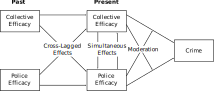
\includegraphics[width=0.9\linewidth]{./figure/ch3/longitudinal_model} 

}

\caption{Potential Effects of Collective Efficacy and Police Efficacy}\label{fig:fclongitudinalmodel}
\end{figure}
I restate my hypotheses here, in the order they will be tested:
\begin{enumerate}
\def\labelenumi{\arabic{enumi}.}
\tightlist
\item
  Police efficacy and collective efficacy moderate each others' effects on crime.
\item
  Police efficacy and collective efficacy are causally ordered. There are two components of this hypothesis:
  \begin{enumerate}
  \def\labelenumii{\alph{enumii}.}
  \tightlist
  \item
    Police efficacy is an antecedent of collective efficacy. This may occur either slowly (lagged effects) or rapidly (simultaneous effect).
  \item
    Collective efficacy is an antecedent of police efficacy. This may occur either slowly (lagged effect) or rapidly (simultaneous effect).
  \end{enumerate}
\end{enumerate}
In the following sections, I briefly describe the data used to test these hypotheses, paying particular attention to measurement, then walk through the estimation approaches at length, discussing how they address potential violations of modeling assumptions.

\hypertarget{data-and-measurement}{%
\section{Data and Measurement}\label{data-and-measurement}}

This chapter uses a two-period neighborhood-level panel data set assembled from the 1995 Project on Human Development in Chicago Neighborhoods Community Survey (PHDCN-CS) (Earls et al. 1999) and the 2003 Chicago Community Adult Health Study (CCAHS) (House et al. 2011). These survey data are augmented with neighborhood measures constructed from indicators in the Longitudinal Tract Data Base (LTDB) (Logan, Xu, and Stults 2014) and police-reported crime from publicly accessible Chicago Police Department records ({Chicago Police Department} 2020). Because the data used here are identical to those used for Chapter \ref{builtenvironment}, they are fully described in Appendix \ref{measures} to minimize redundancy. That appendix describes the data sources and details the measurement strategies which apply to both chapters. Table \ref{tab:fcdescrip} depicts descriptive statistics for the measures used in this chapter. The following section details methods specific to this chapter.

\providecommand{\docline}[3]{\noalign{\global\setlength{\arrayrulewidth}{#1}}\arrayrulecolor[HTML]{#2}\cline{#3}}

\setlength{\tabcolsep}{2pt}

\renewcommand*{\arraystretch}{1}
\begin{longtable}[c]{cccccc}

\caption{\label{tab:fcdescrip} Descriptive Statistics}\label{tab:unnamed-chunk-4}\\

\hhline{>{\arrayrulecolor[HTML]{000000}\global\arrayrulewidth=1pt}->{\arrayrulecolor[HTML]{000000}\global\arrayrulewidth=1pt}->{\arrayrulecolor[HTML]{000000}\global\arrayrulewidth=1pt}->{\arrayrulecolor[HTML]{000000}\global\arrayrulewidth=1pt}->{\arrayrulecolor[HTML]{000000}\global\arrayrulewidth=1pt}->{\arrayrulecolor[HTML]{000000}\global\arrayrulewidth=1pt}-}

\multicolumn{1}{!{\color[HTML]{000000}\vrule width 0pt}>{}l}{\fontsize{11}{11}\selectfont{\textcolor[HTML]{000000}{\global\setmainfont{Latin Modern Roman}Measure}}} & \multicolumn{1}{!{\color[HTML]{000000}\vrule width 0pt}>{}c}{\fontsize{11}{11}\selectfont{\textcolor[HTML]{000000}{\global\setmainfont{Latin Modern Roman}Mean}}} & \multicolumn{1}{!{\color[HTML]{000000}\vrule width 0pt}>{}c}{\fontsize{11}{11}\selectfont{\textcolor[HTML]{000000}{\global\setmainfont{Latin Modern Roman}SD}}} & \multicolumn{1}{!{\color[HTML]{000000}\vrule width 0pt}>{}c}{\fontsize{11}{11}\selectfont{\textcolor[HTML]{000000}{\global\setmainfont{Latin Modern Roman}Min}}} & \multicolumn{1}{!{\color[HTML]{000000}\vrule width 0pt}>{}c}{\fontsize{11}{11}\selectfont{\textcolor[HTML]{000000}{\global\setmainfont{Latin Modern Roman}Density}}} & \multicolumn{1}{!{\color[HTML]{000000}\vrule width 0pt}>{}c!{\color[HTML]{000000}\vrule width 0pt}}{\fontsize{11}{11}\selectfont{\textcolor[HTML]{000000}{\global\setmainfont{Latin Modern Roman}Max}}} \\

\noalign{\global\setlength{\arrayrulewidth}{0.5pt}}\arrayrulecolor[HTML]{000000}\cline{1-6}

\endfirsthead

\hhline{>{\arrayrulecolor[HTML]{000000}\global\arrayrulewidth=1pt}->{\arrayrulecolor[HTML]{000000}\global\arrayrulewidth=1pt}->{\arrayrulecolor[HTML]{000000}\global\arrayrulewidth=1pt}->{\arrayrulecolor[HTML]{000000}\global\arrayrulewidth=1pt}->{\arrayrulecolor[HTML]{000000}\global\arrayrulewidth=1pt}->{\arrayrulecolor[HTML]{000000}\global\arrayrulewidth=1pt}-}

\multicolumn{1}{!{\color[HTML]{000000}\vrule width 0pt}>{}l}{\fontsize{11}{11}\selectfont{\textcolor[HTML]{000000}{\global\setmainfont{Latin Modern Roman}Measure}}} & \multicolumn{1}{!{\color[HTML]{000000}\vrule width 0pt}>{}c}{\fontsize{11}{11}\selectfont{\textcolor[HTML]{000000}{\global\setmainfont{Latin Modern Roman}Mean}}} & \multicolumn{1}{!{\color[HTML]{000000}\vrule width 0pt}>{}c}{\fontsize{11}{11}\selectfont{\textcolor[HTML]{000000}{\global\setmainfont{Latin Modern Roman}SD}}} & \multicolumn{1}{!{\color[HTML]{000000}\vrule width 0pt}>{}c}{\fontsize{11}{11}\selectfont{\textcolor[HTML]{000000}{\global\setmainfont{Latin Modern Roman}Min}}} & \multicolumn{1}{!{\color[HTML]{000000}\vrule width 0pt}>{}c}{\fontsize{11}{11}\selectfont{\textcolor[HTML]{000000}{\global\setmainfont{Latin Modern Roman}Density}}} & \multicolumn{1}{!{\color[HTML]{000000}\vrule width 0pt}>{}c!{\color[HTML]{000000}\vrule width 0pt}}{\fontsize{11}{11}\selectfont{\textcolor[HTML]{000000}{\global\setmainfont{Latin Modern Roman}Max}}} \\

\noalign{\global\setlength{\arrayrulewidth}{0.5pt}}\arrayrulecolor[HTML]{000000}\cline{1-6}\endhead



\multicolumn{1}{!{\color[HTML]{000000}\vrule width 0pt}>{}l}{\fontsize{11}{11}\selectfont{\textcolor[HTML]{000000}{\global\setmainfont{Latin Modern Roman}Homicide}}} & \multicolumn{1}{!{\color[HTML]{000000}\vrule width 0pt}>{}c}{\fontsize{11}{11}\selectfont{\textcolor[HTML]{000000}{\global\setmainfont{Latin Modern Roman}2.03}}} & \multicolumn{1}{!{\color[HTML]{000000}\vrule width 0pt}>{}c}{\fontsize{11}{11}\selectfont{\textcolor[HTML]{000000}{\global\setmainfont{Latin Modern Roman}2.39}}} & \multicolumn{1}{!{\color[HTML]{000000}\vrule width 0pt}>{}c}{\fontsize{11}{11}\selectfont{\textcolor[HTML]{000000}{\global\setmainfont{Latin Modern Roman}0.00}}} & \multicolumn{1}{!{\color[HTML]{000000}\vrule width 0pt}>{}c}{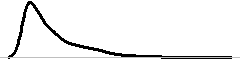
\includegraphics[width=0.8in, height=0.2in]{thesis_files/figure-latex/unnamed-chunk-4-1.png}} & \multicolumn{1}{!{\color[HTML]{000000}\vrule width 0pt}>{}c!{\color[HTML]{000000}\vrule width 0pt}}{\fontsize{11}{11}\selectfont{\textcolor[HTML]{000000}{\global\setmainfont{Latin Modern Roman}15.00}}} \\





\multicolumn{1}{!{\color[HTML]{000000}\vrule width 0pt}>{}l}{\fontsize{11}{11}\selectfont{\textcolor[HTML]{000000}{\global\setmainfont{Latin Modern Roman}Perceived Violence}}} & \multicolumn{1}{!{\color[HTML]{000000}\vrule width 0pt}>{}c}{\fontsize{11}{11}\selectfont{\textcolor[HTML]{000000}{\global\setmainfont{Latin Modern Roman}0.00}}} & \multicolumn{1}{!{\color[HTML]{000000}\vrule width 0pt}>{}c}{\fontsize{11}{11}\selectfont{\textcolor[HTML]{000000}{\global\setmainfont{Latin Modern Roman}1.00}}} & \multicolumn{1}{!{\color[HTML]{000000}\vrule width 0pt}>{}c}{\fontsize{11}{11}\selectfont{\textcolor[HTML]{000000}{\global\setmainfont{Latin Modern Roman}-1.95}}} & \multicolumn{1}{!{\color[HTML]{000000}\vrule width 0pt}>{}c}{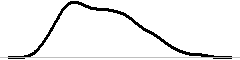
\includegraphics[width=0.8in, height=0.2in]{thesis_files/figure-latex/unnamed-chunk-4-2.png}} & \multicolumn{1}{!{\color[HTML]{000000}\vrule width 0pt}>{}c!{\color[HTML]{000000}\vrule width 0pt}}{\fontsize{11}{11}\selectfont{\textcolor[HTML]{000000}{\global\setmainfont{Latin Modern Roman}2.94}}} \\





\multicolumn{1}{!{\color[HTML]{000000}\vrule width 0pt}>{}l}{\fontsize{11}{11}\selectfont{\textcolor[HTML]{000000}{\global\setmainfont{Latin Modern Roman}Victimization}}} & \multicolumn{1}{!{\color[HTML]{000000}\vrule width 0pt}>{}c}{\fontsize{11}{11}\selectfont{\textcolor[HTML]{000000}{\global\setmainfont{Latin Modern Roman}0.00}}} & \multicolumn{1}{!{\color[HTML]{000000}\vrule width 0pt}>{}c}{\fontsize{11}{11}\selectfont{\textcolor[HTML]{000000}{\global\setmainfont{Latin Modern Roman}1.00}}} & \multicolumn{1}{!{\color[HTML]{000000}\vrule width 0pt}>{}c}{\fontsize{11}{11}\selectfont{\textcolor[HTML]{000000}{\global\setmainfont{Latin Modern Roman}-2.08}}} & \multicolumn{1}{!{\color[HTML]{000000}\vrule width 0pt}>{}c}{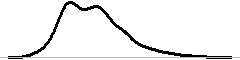
\includegraphics[width=0.8in, height=0.2in]{thesis_files/figure-latex/unnamed-chunk-4-3.png}} & \multicolumn{1}{!{\color[HTML]{000000}\vrule width 0pt}>{}c!{\color[HTML]{000000}\vrule width 0pt}}{\fontsize{11}{11}\selectfont{\textcolor[HTML]{000000}{\global\setmainfont{Latin Modern Roman}3.79}}} \\





\multicolumn{1}{!{\color[HTML]{000000}\vrule width 0pt}>{}l}{\fontsize{11}{11}\selectfont{\textcolor[HTML]{000000}{\global\setmainfont{Latin Modern Roman}Violent Crime}}} & \multicolumn{1}{!{\color[HTML]{000000}\vrule width 0pt}>{}c}{\fontsize{11}{11}\selectfont{\textcolor[HTML]{000000}{\global\setmainfont{Latin Modern Roman}0.00}}} & \multicolumn{1}{!{\color[HTML]{000000}\vrule width 0pt}>{}c}{\fontsize{11}{11}\selectfont{\textcolor[HTML]{000000}{\global\setmainfont{Latin Modern Roman}1.00}}} & \multicolumn{1}{!{\color[HTML]{000000}\vrule width 0pt}>{}c}{\fontsize{11}{11}\selectfont{\textcolor[HTML]{000000}{\global\setmainfont{Latin Modern Roman}-1.71}}} & \multicolumn{1}{!{\color[HTML]{000000}\vrule width 0pt}>{}c}{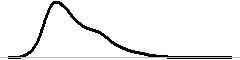
\includegraphics[width=0.8in, height=0.2in]{thesis_files/figure-latex/unnamed-chunk-4-4.png}} & \multicolumn{1}{!{\color[HTML]{000000}\vrule width 0pt}>{}c!{\color[HTML]{000000}\vrule width 0pt}}{\fontsize{11}{11}\selectfont{\textcolor[HTML]{000000}{\global\setmainfont{Latin Modern Roman}4.92}}} \\





\multicolumn{1}{!{\color[HTML]{000000}\vrule width 0pt}>{}l}{\fontsize{11}{11}\selectfont{\textcolor[HTML]{000000}{\global\setmainfont{Latin Modern Roman}Collective Efficacy}}} & \multicolumn{1}{!{\color[HTML]{000000}\vrule width 0pt}>{}c}{\fontsize{11}{11}\selectfont{\textcolor[HTML]{000000}{\global\setmainfont{Latin Modern Roman}0.00}}} & \multicolumn{1}{!{\color[HTML]{000000}\vrule width 0pt}>{}c}{\fontsize{11}{11}\selectfont{\textcolor[HTML]{000000}{\global\setmainfont{Latin Modern Roman}1.00}}} & \multicolumn{1}{!{\color[HTML]{000000}\vrule width 0pt}>{}c}{\fontsize{11}{11}\selectfont{\textcolor[HTML]{000000}{\global\setmainfont{Latin Modern Roman}-3.64}}} & \multicolumn{1}{!{\color[HTML]{000000}\vrule width 0pt}>{}c}{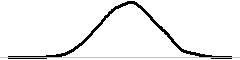
\includegraphics[width=0.8in, height=0.2in]{thesis_files/figure-latex/unnamed-chunk-4-5.png}} & \multicolumn{1}{!{\color[HTML]{000000}\vrule width 0pt}>{}c!{\color[HTML]{000000}\vrule width 0pt}}{\fontsize{11}{11}\selectfont{\textcolor[HTML]{000000}{\global\setmainfont{Latin Modern Roman}3.00}}} \\





\multicolumn{1}{!{\color[HTML]{000000}\vrule width 0pt}>{}l}{\fontsize{11}{11}\selectfont{\textcolor[HTML]{000000}{\global\setmainfont{Latin Modern Roman}Police Efficacy}}} & \multicolumn{1}{!{\color[HTML]{000000}\vrule width 0pt}>{}c}{\fontsize{11}{11}\selectfont{\textcolor[HTML]{000000}{\global\setmainfont{Latin Modern Roman}0.00}}} & \multicolumn{1}{!{\color[HTML]{000000}\vrule width 0pt}>{}c}{\fontsize{11}{11}\selectfont{\textcolor[HTML]{000000}{\global\setmainfont{Latin Modern Roman}1.00}}} & \multicolumn{1}{!{\color[HTML]{000000}\vrule width 0pt}>{}c}{\fontsize{11}{11}\selectfont{\textcolor[HTML]{000000}{\global\setmainfont{Latin Modern Roman}-3.18}}} & \multicolumn{1}{!{\color[HTML]{000000}\vrule width 0pt}>{}c}{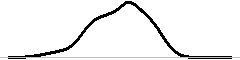
\includegraphics[width=0.8in, height=0.2in]{thesis_files/figure-latex/unnamed-chunk-4-6.png}} & \multicolumn{1}{!{\color[HTML]{000000}\vrule width 0pt}>{}c!{\color[HTML]{000000}\vrule width 0pt}}{\fontsize{11}{11}\selectfont{\textcolor[HTML]{000000}{\global\setmainfont{Latin Modern Roman}3.19}}} \\





\multicolumn{1}{!{\color[HTML]{000000}\vrule width 0pt}>{}l}{\fontsize{11}{11}\selectfont{\textcolor[HTML]{000000}{\global\setmainfont{Latin Modern Roman}Neighboring}}} & \multicolumn{1}{!{\color[HTML]{000000}\vrule width 0pt}>{}c}{\fontsize{11}{11}\selectfont{\textcolor[HTML]{000000}{\global\setmainfont{Latin Modern Roman}0.00}}} & \multicolumn{1}{!{\color[HTML]{000000}\vrule width 0pt}>{}c}{\fontsize{11}{11}\selectfont{\textcolor[HTML]{000000}{\global\setmainfont{Latin Modern Roman}1.00}}} & \multicolumn{1}{!{\color[HTML]{000000}\vrule width 0pt}>{}c}{\fontsize{11}{11}\selectfont{\textcolor[HTML]{000000}{\global\setmainfont{Latin Modern Roman}-3.61}}} & \multicolumn{1}{!{\color[HTML]{000000}\vrule width 0pt}>{}c}{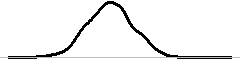
\includegraphics[width=0.8in, height=0.2in]{thesis_files/figure-latex/unnamed-chunk-4-7.png}} & \multicolumn{1}{!{\color[HTML]{000000}\vrule width 0pt}>{}c!{\color[HTML]{000000}\vrule width 0pt}}{\fontsize{11}{11}\selectfont{\textcolor[HTML]{000000}{\global\setmainfont{Latin Modern Roman}4.41}}} \\





\multicolumn{1}{!{\color[HTML]{000000}\vrule width 0pt}>{}l}{\fontsize{11}{11}\selectfont{\textcolor[HTML]{000000}{\global\setmainfont{Latin Modern Roman}Attachment}}} & \multicolumn{1}{!{\color[HTML]{000000}\vrule width 0pt}>{}c}{\fontsize{11}{11}\selectfont{\textcolor[HTML]{000000}{\global\setmainfont{Latin Modern Roman}0.00}}} & \multicolumn{1}{!{\color[HTML]{000000}\vrule width 0pt}>{}c}{\fontsize{11}{11}\selectfont{\textcolor[HTML]{000000}{\global\setmainfont{Latin Modern Roman}1.00}}} & \multicolumn{1}{!{\color[HTML]{000000}\vrule width 0pt}>{}c}{\fontsize{11}{11}\selectfont{\textcolor[HTML]{000000}{\global\setmainfont{Latin Modern Roman}-2.91}}} & \multicolumn{1}{!{\color[HTML]{000000}\vrule width 0pt}>{}c}{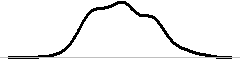
\includegraphics[width=0.8in, height=0.2in]{thesis_files/figure-latex/unnamed-chunk-4-8.png}} & \multicolumn{1}{!{\color[HTML]{000000}\vrule width 0pt}>{}c!{\color[HTML]{000000}\vrule width 0pt}}{\fontsize{11}{11}\selectfont{\textcolor[HTML]{000000}{\global\setmainfont{Latin Modern Roman}2.73}}} \\





\multicolumn{1}{!{\color[HTML]{000000}\vrule width 0pt}>{}l}{\fontsize{11}{11}\selectfont{\textcolor[HTML]{000000}{\global\setmainfont{Latin Modern Roman}Disadvantage}}} & \multicolumn{1}{!{\color[HTML]{000000}\vrule width 0pt}>{}c}{\fontsize{11}{11}\selectfont{\textcolor[HTML]{000000}{\global\setmainfont{Latin Modern Roman}0.00}}} & \multicolumn{1}{!{\color[HTML]{000000}\vrule width 0pt}>{}c}{\fontsize{11}{11}\selectfont{\textcolor[HTML]{000000}{\global\setmainfont{Latin Modern Roman}1.00}}} & \multicolumn{1}{!{\color[HTML]{000000}\vrule width 0pt}>{}c}{\fontsize{11}{11}\selectfont{\textcolor[HTML]{000000}{\global\setmainfont{Latin Modern Roman}-2.24}}} & \multicolumn{1}{!{\color[HTML]{000000}\vrule width 0pt}>{}c}{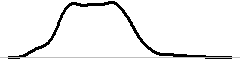
\includegraphics[width=0.8in, height=0.2in]{thesis_files/figure-latex/unnamed-chunk-4-9.png}} & \multicolumn{1}{!{\color[HTML]{000000}\vrule width 0pt}>{}c!{\color[HTML]{000000}\vrule width 0pt}}{\fontsize{11}{11}\selectfont{\textcolor[HTML]{000000}{\global\setmainfont{Latin Modern Roman}3.86}}} \\





\multicolumn{1}{!{\color[HTML]{000000}\vrule width 0pt}>{}l}{\fontsize{11}{11}\selectfont{\textcolor[HTML]{000000}{\global\setmainfont{Latin Modern Roman}Stability}}} & \multicolumn{1}{!{\color[HTML]{000000}\vrule width 0pt}>{}c}{\fontsize{11}{11}\selectfont{\textcolor[HTML]{000000}{\global\setmainfont{Latin Modern Roman}0.00}}} & \multicolumn{1}{!{\color[HTML]{000000}\vrule width 0pt}>{}c}{\fontsize{11}{11}\selectfont{\textcolor[HTML]{000000}{\global\setmainfont{Latin Modern Roman}1.00}}} & \multicolumn{1}{!{\color[HTML]{000000}\vrule width 0pt}>{}c}{\fontsize{11}{11}\selectfont{\textcolor[HTML]{000000}{\global\setmainfont{Latin Modern Roman}-2.38}}} & \multicolumn{1}{!{\color[HTML]{000000}\vrule width 0pt}>{}c}{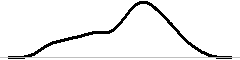
\includegraphics[width=0.8in, height=0.2in]{thesis_files/figure-latex/unnamed-chunk-4-10.png}} & \multicolumn{1}{!{\color[HTML]{000000}\vrule width 0pt}>{}c!{\color[HTML]{000000}\vrule width 0pt}}{\fontsize{11}{11}\selectfont{\textcolor[HTML]{000000}{\global\setmainfont{Latin Modern Roman}1.95}}} \\





\multicolumn{1}{!{\color[HTML]{000000}\vrule width 0pt}>{}l}{\fontsize{11}{11}\selectfont{\textcolor[HTML]{000000}{\global\setmainfont{Latin Modern Roman}Hispanic/Immigrant}}} & \multicolumn{1}{!{\color[HTML]{000000}\vrule width 0pt}>{}c}{\fontsize{11}{11}\selectfont{\textcolor[HTML]{000000}{\global\setmainfont{Latin Modern Roman}0.00}}} & \multicolumn{1}{!{\color[HTML]{000000}\vrule width 0pt}>{}c}{\fontsize{11}{11}\selectfont{\textcolor[HTML]{000000}{\global\setmainfont{Latin Modern Roman}1.00}}} & \multicolumn{1}{!{\color[HTML]{000000}\vrule width 0pt}>{}c}{\fontsize{11}{11}\selectfont{\textcolor[HTML]{000000}{\global\setmainfont{Latin Modern Roman}-2.45}}} & \multicolumn{1}{!{\color[HTML]{000000}\vrule width 0pt}>{}c}{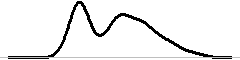
\includegraphics[width=0.8in, height=0.2in]{thesis_files/figure-latex/unnamed-chunk-4-11.png}} & \multicolumn{1}{!{\color[HTML]{000000}\vrule width 0pt}>{}c!{\color[HTML]{000000}\vrule width 0pt}}{\fontsize{11}{11}\selectfont{\textcolor[HTML]{000000}{\global\setmainfont{Latin Modern Roman}2.63}}} \\

\noalign{\global\setlength{\arrayrulewidth}{1pt}}\arrayrulecolor[HTML]{000000}\cline{1-6}

\end{longtable}
I conceptualize police efficacy as a neighborhood-level capacity to call upon police to engage in social control in accordance with the expectations of residents. That is, a neighborhood with high police efficacy is one where residents believe the police are capable of combatting crime, will respond and investigate when called, and will treat both callers and suspects fairly and respectfully. This definition encompasses both effectiveness and legitimacy, which are commonly found to be distinct in research on policing procedures (Tyler 2006), though Sampson and Bartusch (1998) combined five measures capturing both effectiveness and legitimacy (as ``police satisfaction'') in their analysis of legal cynicism using the PHDCN-CS. The same scale was also used by Silver and Miller (2004). One prominent study combined indicators of police efficacy into a legal cynicism construct (Kirk and Matsuda 2011). As documented in Appendix \ref{legalcynicism}, I found evidence in support of separating police efficacy from legal cynicism and omitting legal cynicism from the overall analysis.

To construct a police efficacy scale, I begin with the five indicators used by Sampson and Bartusch (1998) and Silver and Miller (2004) which encompass responsiveness, effectiveness in maintaining order and controlling crime, and fair treatment of both victims and suspects (see Appendix \ref{measures}). To these prior measures, I add three indicators reflecting resident perceptions of change in police protection over the last 5 years, excessive use of force, and failure to patrol and respond to calls. All eight measures are used together as factor analysis suggests the indicators are not clearly separable into different effectiveness and legitimacy factors, though they are separable from the indicators of collective efficacy---informal social control expectations and cohesion and trust. The 2003 police efficacy measure constructed from the CCAHS includes only three measures which encompass effectiveness, responsiveness, and fairness.

The crime measures used are police-reported homicide, survey-reported perceived violence, survey-reported violent victimization, and violent crime. The violent crime measure is a composite of two different measures. In 2003 the measure is constructed from the sum of homicides, robberies, and aggravated assaults and batteries in 2003 divided by the year 2000 population. In 1995, I use the violent crime measure from the PHDCN-CS aggregate NC-level dataset from ICPSR (Earls et al. 1999). This measure is undocumented, so it is uncertain if it represents police-reported violent crime like the constructed 2003 measure or some other composite measure such as the one used by Sampson and Bartusch (1998).\footnote{The 1995 violent crime measure is correlated approximately 0.89 with the sum of the standardized homicide, perceived violence, and victimization measures, which is the index construction method described by Sampson and Bartusch (1998). Performing the same operation on the 2003 data yields a correlation of 0.53 with the police-report based violent crime measure. I thus strongly suspect this is indeed the index from Sampson and Bartusch (1998).} The interwave correlation for the two violent crime measures is 0.61 which is higher than that for any of the other crime measures. It is, however, more strongly correlated with the other 1995 crime measures than the 2003 violent crime measure is with the other 2003 measures. Thus the 1995 violent crime measure should be viewed cautiously. Unfortunately, I have no alternative measure for 1995 violent crime as the PHDCN does not provide one and the Chicago Police Department only provides data from the year 2000 onward. The ICPSR release of the PHDCN-CS is also missing values for homicide and violent crime in 1995 for one neighborhood. This observation is dropped in random- and fixed-effects models but included via full-information maximum likelihood in structural equation models. Inclusion has no impact on estimates.

\hypertarget{methods-and-results}{%
\section{Methods and Results}\label{methods-and-results}}

I use three general estimation strategies to test my hypotheses. I use random- and fixed-effects panel models test Hypothesis 1: collective efficacy and police efficacy moderate each other's effects on crime. Before testing this moderation hypothesis, I use two specifications to evaluate conditional associations of collective efficacy and police efficacy with crime, both overall and within each panel year. Moderation is unlikely to be found if those conditional associations are weak or absent---as appears to be the case in 2003.

Hypothesis 2, that police efficacy and collective efficacy are causally ordered, is tested using two forms of structural equations: cross-lagged panel models and a simultaneous effect instrumental variables model. These models allow evaluating the directionality of associations using temporal ordering and assumptions about conditional independence. Using both types of model helps address the possibility that causal effects operate at different rates: cross-lagged models assume an 8-year lagged effect while the instrumental variables model assume they operate over the short term. Both forms of structural equation relax the assumption of time-invariant parameters by permitting the effects of collective efficacy and police efficacy on crime to differ in 1995 and 2003.

\hypertarget{random--and-fixed-effects-panel-models}{%
\subsection{Random- and Fixed-Effects Panel Models}\label{random--and-fixed-effects-panel-models}}

The first estimation strategy uses random- and fixed-effects panel models to estimate the conditional direct effects of collective efficacy and police efficacy on crime and test for moderation of these effects. These models correspond to the arrows in Figure \ref{fig:fclongitudinalmodel} from collective efficacy and police efficacy to crime and the labeled moderation pathways. For these models, I first describe the estimation approaches and model specifications before discussing results.

For all four outcomes---homicide, victimization, violent crime, and perceived violence---I use four estimation approaches, and, within each approach, either three or four different specifications. These models make the assumption collective efficacy and policy efficacy have independent simultaneous effects on crime and neither is a mediator for the others' effects. If, for instance, police efficacy influences crime and is in part the result of collective efficacy, including it in a model alongside collective efficacy will attenuate the estimated effect of collective efficacy on crime. This is conditioning on a post-treatment mediator---controlling, in effect, for a mechanism of the causal variable of interest. If this attenuation occurs, however, it suggests police efficacy is either a mediator for collective efficacy or, if not, the effect of collective efficacy on crime is partly spurious, and police efficacy is an omitted variable in past studies.

\hypertarget{random-effects}{%
\subsubsection{Random effects}\label{random-effects}}

The first estimation approach is a simple panel regression with random intercepts for neighborhoods. For homicide, this is a Poisson regression with a population exposure term for which the coefficient is fixed to 1.\footnote{Respecifying this as a negative binomial model reveals no evidence of overdispersion.} For the other outcomes, this is a standard linear regression. Identification of treatment effects in this approach relies on strong ignorability given covariates---adjustment for anything causally antecedent to both crime and either collective efficacy or police efficacy (see Lanfear, Matsueda, and Beach 2020). This includes both time varying and time stable confounders. An implication of this assumption is that we must assume there is no effect of past crime on present crime except through included covariates. If there is a direct effect of past crime on present crime or one mediated by any omitted variable, it will bias estimates for collective efficacy and police efficacy, because past research strongly suggests they are influenced by crime (Sampson 2012; Sampson and Bartusch 1998).

\hypertarget{lag-homicide}{%
\subsubsection{Lag homicide}\label{lag-homicide}}

The second estimation approach partially relaxes the assumption that past crime does not predict present crime---either directly or via an omitted mediator---by using the lag homicide rate as a predictor. Due to the absence of 1990 measures for any other outcomes, homicide must be used for lagged crime across all specifications. Note that while this is a conventional dynamic panel estimator for the homicide outcome (Wooldridge 2010), it is not for the other outcomes.\footnote{One might think of it as a dynamic panel model with unmodeled measurement error in the predictor.} Rather, I am making the assumption that homicide captures most or all effects of past crime regardless of the outcome under consideration. Auxiliary models predicting second wave crime outcomes suggest this is the case except for perceived violence, where 1995 perceived violence dominates homicide in predicting 2003 perceived violence. However, perceived violence in 1995 has no substantively or statistically significant relationship with 2003 collective efficacy or police efficacy, so it is possible it may not threaten identification. These models retain the random effects from the prior specification, except in the case of violent crime where a standard linear model with heteroskedasticity and autocorrelation consistent standard errors is used due to is insufficient inter-neighborhood residual variation to stably estimate random effects.

\hypertarget{fixed-effects}{%
\subsubsection{Fixed effects}\label{fixed-effects}}

We can relax the assumption that there are no time-stable omitted confounders using unit fixed effects specifications. With a two-wave fixed effects specification, we are estimating the relationship between deviations from unit-level means of the regressors and outcomes. This specification produces two major limitations: efficiency and inability to model stability over time. Fixed effects specifications use an additional degree of freedom for every observation, resulting in larger standard errors. They also cannot model observations for which there was no change between time periods. This does not result in bias, but does diminish statistical power. This second limitation is particularly problematic for rare outcomes like homicide. In the present case, 111 of the 342 neighborhoods with homicide data experienced the same number of homicides in both waves, including 75 which experienced none in either wave.\footnote{If homicide is specified as a rate, rather than count, it is possible to recover the non-zero values due to changing population size (denominator). I chose not to do this as I would still lose over a quarter of all neighborhoods.} Due to the large number of observations that would be dropped due to fixed effects, tests would be quite underpowered. Consequently, I do not model homicide using this specification. The other outcomes are modeled using the fixed-effects ordinary least squares regressions from the \texttt{fixest} R package (Bergé 2018) with heteroskedasticity and autocorrelation consistent standard errors from the \texttt{sandwich} package (Zeileis, Köll, and Graham 2020).

Unit fixed effects models make the assumptions that past treatments (1) do not influence current outcomes (except via included covariates) and (2) past outcomes do not influence treatment (Imai and Kim 2019). Chapter 2 of this dissertation suggests the first assumption is violated in the case of collective efficacy, as past collective efficacy may exert crime-controlling effects via the built environment. This is typically addressed using lagged treatment variables (Imai and Kim 2019). Chapter \ref{builtenvironment} indicates these effects may be modest in magnitude, however. Canonical research on collective efficacy suggests the second assumption is also violated due to feedback effects of crime on collective efficacy (e.g., Sampson 2012). This is typically addressed using a lagged outcome variable in an instrumental variables framework such as the Arellano-Bond estimator (Arellano and Bond 1991; Imai and Kim 2019). In the present case, neither of these potential violations may be addressed with these approaches as there are insufficient lags available of either the treatment or outcome.

\hypertarget{gaussian-markov-random-field}{%
\subsubsection{Gaussian Markov random field}\label{gaussian-markov-random-field}}

It is reasonable to expect that crime rates in one neighborhood may depend on what occurs in other nearby neighborhoods. Spatial dependence in general will bias estimates of standard errors, and some forms---interference---will also threaten identification of treatment effects such as for collective efficacy. Moran's I tests of residual spatial dependence indicate most of the random effects specifications exhibit spatial dependence (but generally not the fixed effects). To address spatial dependence, my next estimation approach uses generalized additive models (GAMs) with a Gaussian Markov random field (MRF) spatial smoother fit using R's \texttt{mgcv} package (Wood 2017). This approach models spatial dependence between observations using a spatial random effect assumed drawn from a normal distribution with a mean equal to the mean of neighboring unit random effects. In MRFs, the ``Markov'' signifies that observations are independent of all non-neighboring observations conditional on their neighbors---like a Markov chain, it is ``memory-less'' as any given state only depends on its immediate antecedents. This independence assumption is relatively weak in many applications and makes large sample estimation tractable. Consequently, GRMFs are one of the most common approaches to spatial statistical modeling (Rue and Held 2005).

\hypertarget{instrumental-variables}{%
\subsubsection{Instrumental variables}\label{instrumental-variables}}

The last approach uses neighboring activities and kinship and friendship ties as instruments for collective efficacy analogous to the approach of Sampson and Raudenbush (1999). Those authors used neighboring activities, kinship and friendship ties, and neighborhood attachment as instruments for the effect of collective efficacy on crime in cross-sectional simultaneous equations using the same 1995 data as the present study. There, they found reciprocal effects between collective efficacy and both homicide and robbery. The attachment to neighborhood measures are unavailable in the 2003 wave, so here I use only neighboring activities and ties. This specification makes the strong and untestable assumption that the only relationship that neighboring activities and friend and kinships ties have with crime are explained by collective efficacy or other included covariates (Morgan and Winship 2015). Fixed effects are retained in this approach except for homicide. Homicide is also transformed into the log of the homicide rate to facilitate using a conventional linear two-stage least squares estimator.

\hypertarget{random--and-fixed-effects-specifications}{%
\subsubsection{Random- and Fixed-Effects Specifications}\label{random--and-fixed-effects-specifications}}

All approaches above were fit with multiple model specifications both to test hypotheses and relax potentially violated assumptions. These specifications are a (1) base specification, (2) a year interaction, (3) a interaction of Collective Efficacy with Police Efficacy, and (4) and specifications 1 through 3 with a spline on disadvantage to adjust for residual nonlinearity.

The base specification predicts the given crime outcome with the two treatments of interest---collective efficacy and police efficacy---and five controls---the three structural measures, population density, and a dummy distinguishing panel waves. This specification is suitable for establishing baseline conditional associations between collective efficacy and police efficacy and crime. Note that the fixed effects specifications retain the year dummy control variable to adjust for overall differences in outcomes across waves. As a result, these are two-way fixed effects (TWFE) specifications. Recent research on TWFE estimators suggest they are problematic for causal inference in data with multiple periods and binary treatments due to these estimators calculating treatment effects in relation to already-treated units and assigning negative weights to some cases (Imai \& Kim 2020). While research is still developing in settings with continuous treatments, this literature suggests these are less of a concern in two-period settings. Further, the present models are completely insensitive to the presence of the year dummy variable.

A limitation of the base specification is that, by fixing parameters to be invariant across waves, it makes the assumption the effects collective efficacy and police efficacy (as well the controls) are identical across waves of the panel. This assumption may be violated for both artificial and natural reasons. First, the much smaller sample size for the CCAHS means the 2003 measures are less precise than the 1995 measures which may artificially attenuate estimates for the second wave. If this is the case, it is arguable whether relaxing parameter invariance is desirable. Forcing invariance might be seen as borrowing information across waves since the first wave is more precisely estimated. Additionally, for police efficacy, the indicators are different between waves and there are only three indicators in 2003 compared to eight in 1995. If this reduced set of indicators does not tap the same dimensions of the underlying construct, we would expect the factor to exhibit a different relationship with crime. Similarly, if fewer indicators translate into less precision, it may further attenuate estimates.

Second, we might expect an actual ``natural'' difference in parameters due to shift in the relative contribution of informal and formal social control actions to rates of crime. This may occur from an increased reliance on invoking police to solve problems across the time period under consideration (Harcourt 2001; Sharkey 2018), or shifts away from conventional informal social control into new formally-mediated means (Carr 2003; Carr 2012). The first alternate specification addresses the possibility of varying effects across waves with interaction terms between survey year and both collective efficacy and police efficacy (but not between collective efficacy and police efficacy).

The third specification includes an interaction term between collective efficacy and police efficacy to permit testing Hypothesis 1: Police efficacy and collective efficacy moderate one-another in their effects on crime. If residents are emboldened to engage in informal social control due to the belief they are supported by effective police, we would expect to see a negative interaction coefficient: At high levels of both collective efficacy and police efficacy, there is an additional crime control benefit. In contrast to my theoretical expectation, if the crime control benefits of higher collective efficacy or police efficacy come mainly when the other is low, we may instead see a positive interaction term: At high levels of both collective efficacy and police efficacy, crime is higher than an additive relationship would predict.

The fourth and final specification is used only in a subset of MRF GAM models. Analysis of model residuals from across all estimators and specifications reveals a nonlinear relationship between disadvantage and crime. These GAM models use a nonlinear transformation of disadvantage via a thin-plate regression spline to address the nonlinear correlation in the residuals (Wood 2017). Thin-plate splines map a predictor on to the outcome via a smooth function with curvature penalized to prevent overfitting. The spline improves model fit notably but appears inconsequential for estimates of collective efficacy and police efficacy and the particular spline shape here is not replicable with any conventional polynomial term of reasonable degree.\footnote{Significant fit improvement was indicated by greater than 6 point reductions in Bayesian Information Criteria values (Raftery 1995) and insignificant combined adjusted quantile tests (Gelman and Hill 2007).} Consequently, the spline model results are presented for comparison, but no similar transformation was attempted in the other approaches. No other covariates appear to display a significant nonlinear association with any of the outcomes.

\hypertarget{random--and-fixed-effects-results}{%
\subsection{Random- and Fixed-Effects Results}\label{random--and-fixed-effects-results}}

Rather than walking through the results for every one of the many estimation approaches and specifications, I graphically display all point estimates of interest and provide a holistic interpretation. Estimates for controls are not presented as they are not substantively meaningful given that collective efficacy and police efficacy are likely mediators of their effects on crime. Figure \ref{fig:fccoefplot} is a full-page illustration of the point estimates for every combination of estimation approach and model specification described above. The top section shows point estimates of the effects of collective efficacy and police efficacy for the base models. The center section shows point estimates for the year interaction models broken out into year-specific estimates. The bottom section shows results from the collective efficacy and police efficacy interaction models where the displayed point estimates are the interaction terms between collective efficacy and police efficacy.

The tight groupings of point estimates indicate they are fairly insensitive to model specification, except when instrumenting collective efficacy using neighboring behavior and kinship and friendship ties. Similarly, the consistent error bars indicate precision is not greatly affected by modeling decisions except in the case of the instrumental variables, and, to a lesser degree, fixed effects. The unstable and imprecise estimates for collective efficacy in the instrumental variable specification may be indicative of weak instruments (Morgan and Winship 2015:303--4).
\begin{figure}

{\centering 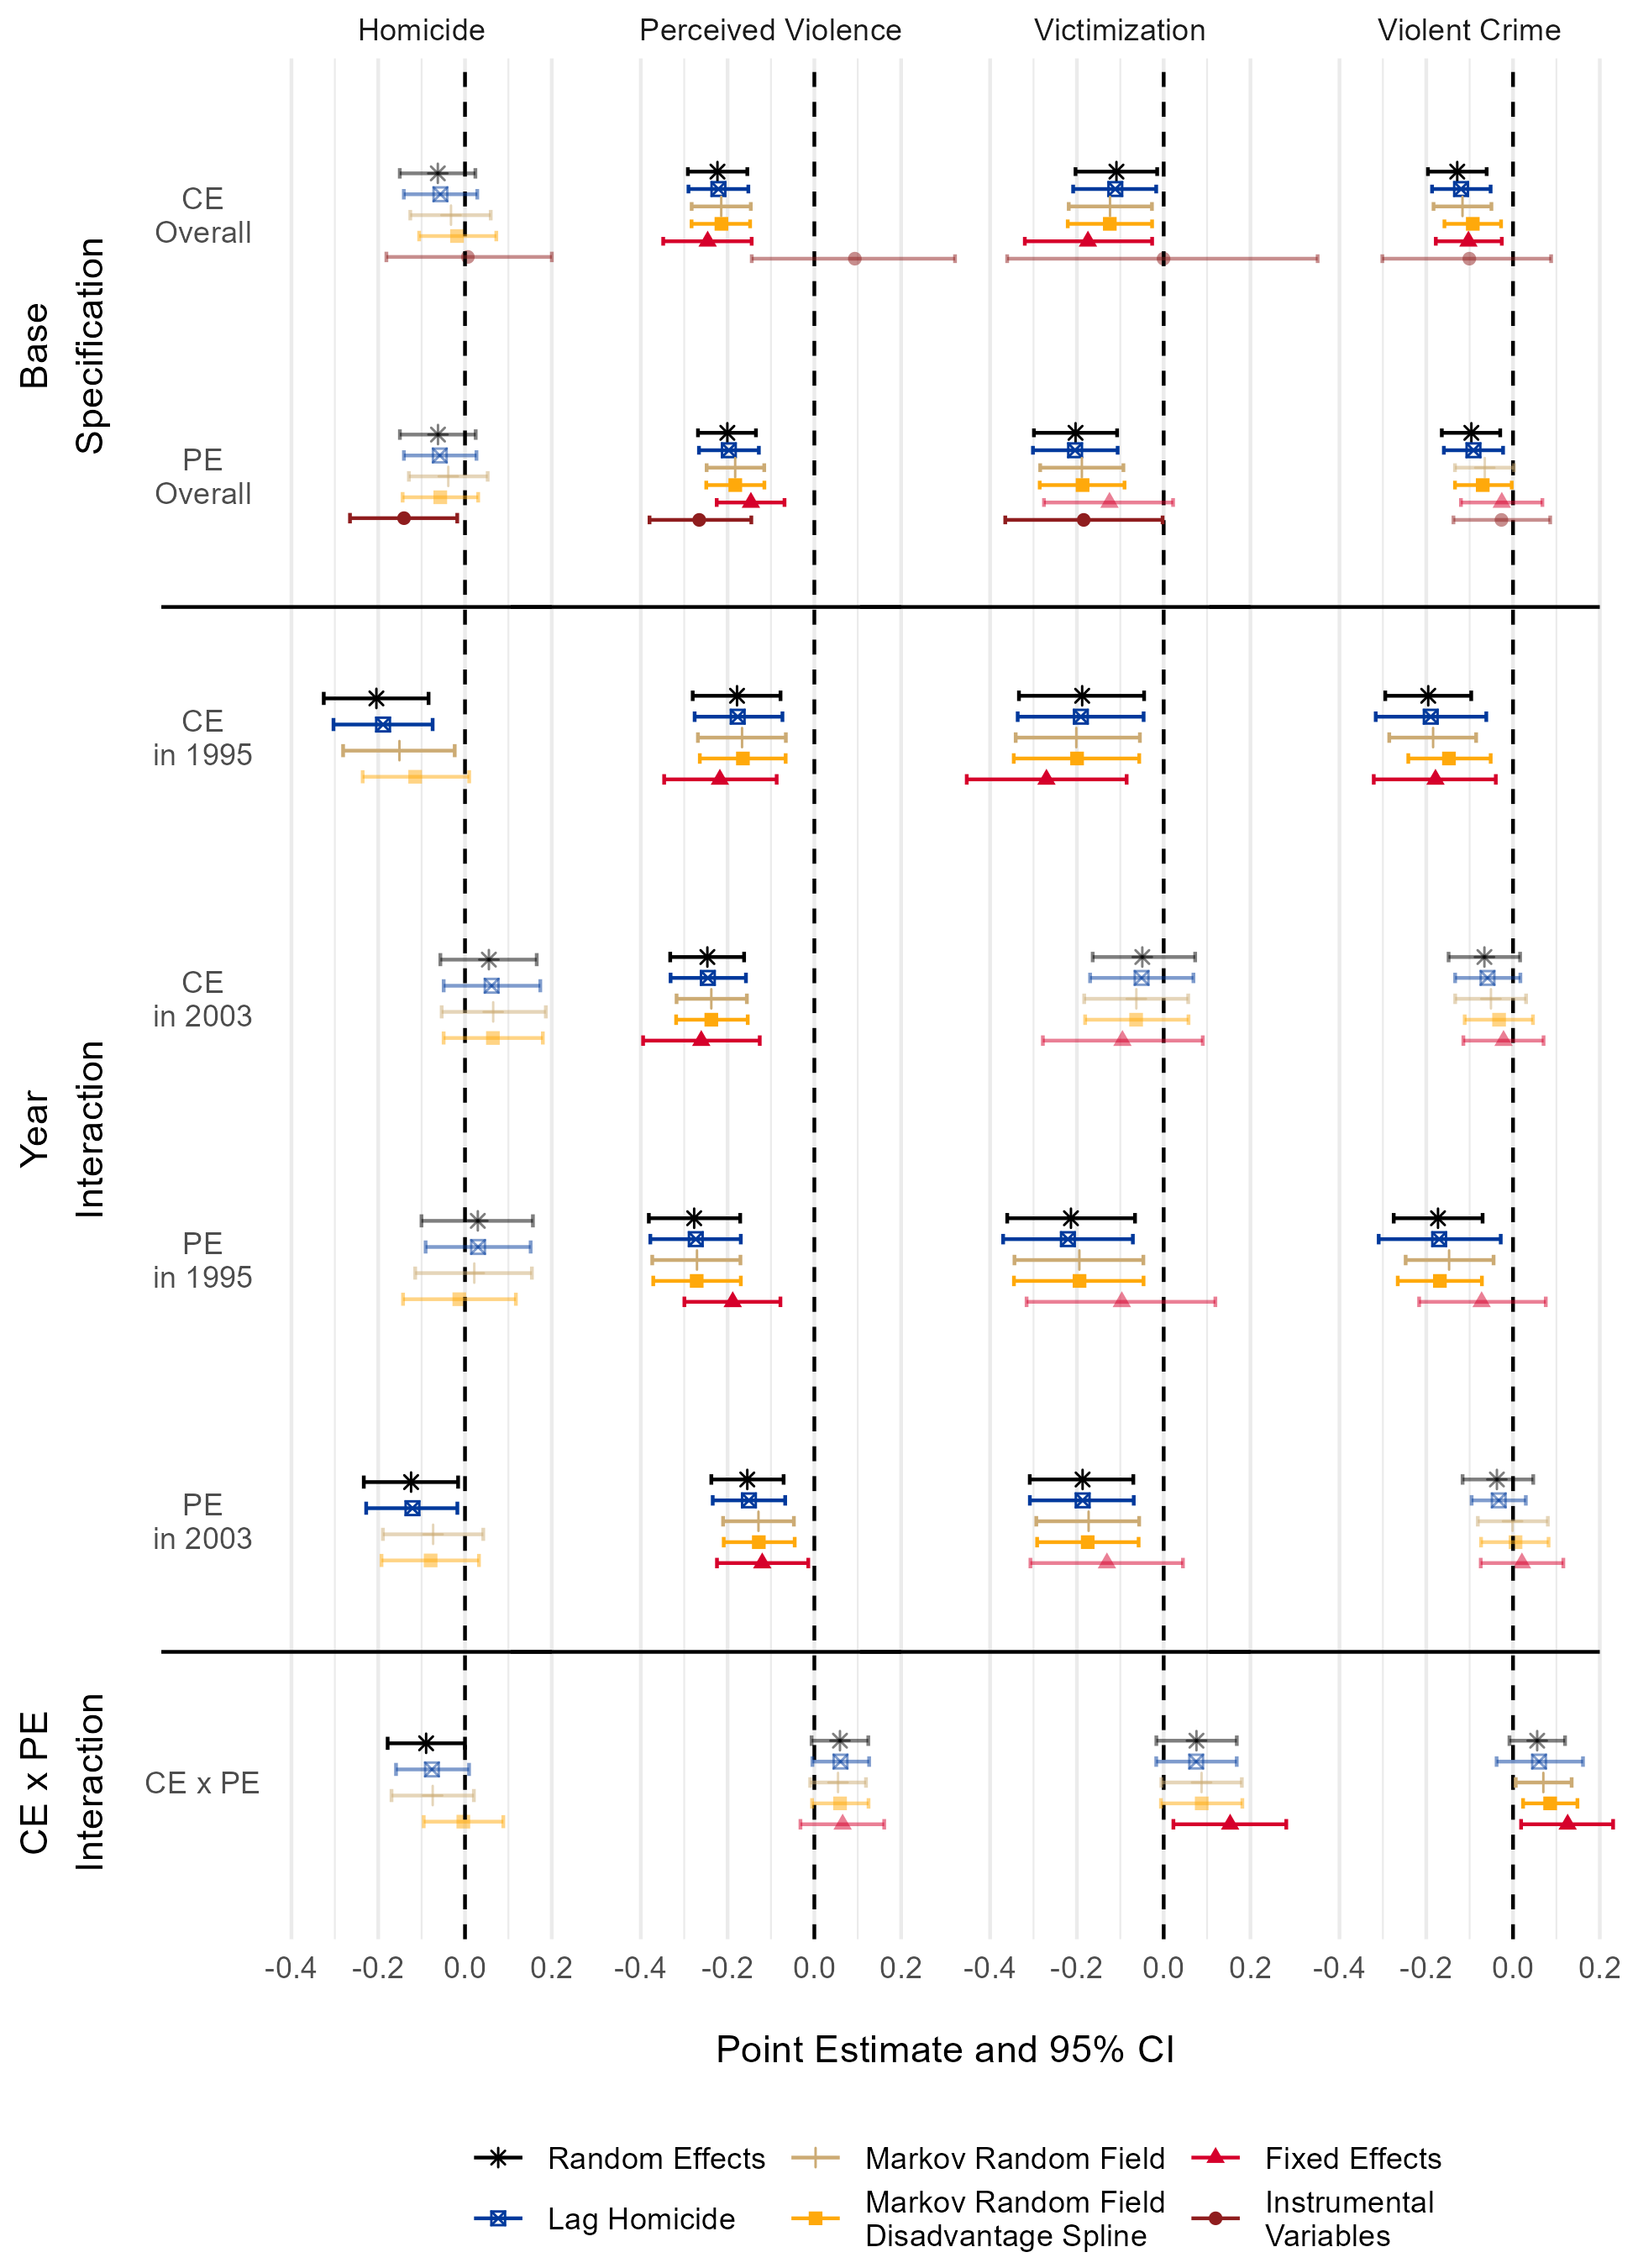
\includegraphics[width=0.8\linewidth]{./figure/ch3/ce_pe_plot_vertical} 

}

\caption{Estimated effects of collective efficacy and police efficacy on four forms of crime from six estimation strategies and four model specifications. Dots are point estimates. Bars are 95\% confidence intervals. Estimates faded out where intervals include zero.}\label{fig:fccoefplot}
\end{figure}
For collective efficacy, in the results indicate an overall modest negative effect on crime, though small and insignificant in the case of homicide. Importantly, this overall effect of collective efficacy appears to be the average of a stronger negative effect in 1995 and, except in the case of perceived violence, a null effect in 2003. This might result if collective efficacy is endogenous to resident perceptions of crime---survey respondents may be basing informal control expectations on perceived crime (Matsueda and Drakulich 2016). The instrumental variables approach which attempts to adjust for this possibility finds null effects and imprecise estimates for collective efficacy. This appears to be due to two factors: (1) collective efficacy effects are present mainly in 1995, and (2) the inclusion of police efficacy attenuates the conditional association of collective efficacy with crime and greatly reduces precision of the estimates in these models. Restricting the model to 1995 and omitting police efficacy results in replication of the collective efficacy effects seen by Sampson and Raudenbush (1999). Assuming the instruments for collective efficacy are relevant and valid, this may occur if police efficacy is a mediator for collective efficacy's effect on crime. If so, including police efficacy in a model of collective efficacy and crime results in included post-treatment variable bias.

For police efficacy, we see similar overall effects to collective efficacy: modest negative effects on crime and a null effect for homicide. Interestingly, introducing instrumental variables for collective efficacy results in a notable strengthening of the police efficacy estimate for perceived violence and homicide. In the year interaction specifications, we again see variation across waves in effects. For homicide, there is no observed police efficacy effect in 1995 and a weak negative effect in 2003, but there is the opposite pattern for violent crime. Perceived violence is relatively stable though stronger in 1995. Victimization is consistent across waves.

In the final pane, we see that the interaction between collective efficacy and police efficacy is, if present, modest in size. Most point estimates are positive, with the exception of homicide, but nearly all estimates are below the chosen threshold of significance. Positive moderation is more pronounced in the typically-conservative fixed-effects models, though this provides only weak evidence for moderation in light of the other estimates.

\hypertarget{causal-sequences}{%
\subsection{Causal Sequences}\label{causal-sequences}}

The next two sets of models are concerned with testing the causal ordering of collective efficacy and police efficacy. I use two strategies: a pair of cross-lagged panel models, which test causal effects between both collective efficacy and police efficacy over time using temporal ordering, and an instrumental variables model, which tests the contemporaneous causal effect of collective efficacy on police efficacy using strong assumptions about conditional independence.

\hypertarget{cross-lagged-panel-models}{%
\subsubsection{Cross-lagged panel models}\label{cross-lagged-panel-models}}

The first modeling approach for causal sequences evaluates the causal ordering between police efficacy and collective efficacy across time periods using cross-lagged panel models. As the primary focus here is not estimating effects on crime---though they are of some interest---I use only the two crime measures assumed to be most accurate: the log-rate of police-reported homicide and empirical Bayes estimates of survey-reported violent victimization. I estimate a system of structural equations with each crime measure. Figure \ref{fig:crosslagmodel} below depicts the homicide model graphically. In these equations, homicide (HOM) or victimization (VICT) is dependent on police efficacy (PE), collective efficacy (CE), and lagged crime, and the three structural neighborhood measures (STR). Collective efficacy and police efficacy depend on the past period's levels of both, the lag of crime, and the three neighborhood structural measures. I also include contemporaneous residual correlations between collective efficacy and police efficacy in both time periods, signified by double-headed arrows. The structural models were estimated using bootstrapped standard errors and full-information maximum likelihood to address a single observation with missing values for 1990 and 1995 homicide.
\begin{figure}

{\centering 
\includegraphics[width=0.6\linewidth]{./figure/ch3/crosslag_model} 

}

\caption{Two-Wave Cross-Lagged Model of Collective Efficacy, Police Efficacy, and Homicide.}\label{fig:crosslagmodel}
\end{figure}
For the equations with 1995 outcomes, I introduce neighboring behavior (NE) as a predictor for contemporaneous collective efficacy, and attachment to neighborhood (AT) as a predictor for both collective efficacy and police efficacy. I omit kinship and friendship ties here as they are not significantly predictive of collective efficacy or police efficacy. There are sufficient degrees of freedom to test the independence restrictions featuring neighboring behavior and attachment. Attachment is strongly related to both police efficacy and collective efficacy, and conditionally independent of crime. Neighboring behavior is associated only with collective efficacy but may be related to 1995 victimization net of the other covariates (\(p=.049\)). The models are insensitive to removing these predictors or allowing them to directly predict victimization. Only neighboring behavior is available in 2003, and it is conditionally independent of victimization and homicide net of the other covariates. Including these additional predictors is not necessary for identifying any paths in the model, rather they are included to be consistent with the instrumental variables model where they are required for identification.\footnote{Note that finding conditional independence between neighboring and exchange and victimization or homicide is not indicative of a satisfied exclusion restriction to use neighboring and exchange as an instrument for collective efficacy's effect on crime. If there is confounding between collective efficacy and either crime outcome, the path from neighboring and exchange to crime is not identified, because collective efficacy is a collider on that path (Morgan and Winship 2015:301--2).} The cross-lagged models are insensitive to excluding neighboring behavior.

Under the assumption of strong ignorability given covariates, these cross-lagged equations allow estimating effects of collective efficacy and police efficacy on each other from 1995 to 2003. Importantly, however, the three structural measures for the 2003 wave are measured in 2000, after 1995 collective efficacy and police efficacy. This will attenuate their estimates if neighborhood sociodemographic characteristics act as a mediator for the intertemporal effects between collective efficacy and police efficacy. To address this, I specified an auxiliary model with endogenous year 2000 structural variables that depend on all prior wave measures and calculated total effects of police efficacy and collective efficacy as the sum of their direct and mediated pathways. Those auxiliary models produce nearly identical results to the primary models.

\hypertarget{cross-lagged-panel-model-results}{%
\subsubsection{Cross-lagged panel model results}\label{cross-lagged-panel-model-results}}

Figure \ref{fig:crosslagresults} depicts selected parameter estimates and standard errors from the two structural models. All estimates are standardized. The crime results roughly mirror those of the prior section. I find victimization is more consistently related to police efficacy, while collective efficacy is a stronger predictor of homicide, though only in 1995. Neither police efficacy nor collective efficacy significantly predict 2003 homicide. More importantly, these models allow us to see the intertemporal associations of these measures. Both systems of equations reveal a similar pattern: Police efficacy in 2003 is conditionally unrelated to 1995 police efficacy, but predicted by 1995 collective efficacy conditional on the structural covariates. This indicates police efficacy is descended from collective efficacy, and thus may mediate its effects on crime. Effective policing may be a proximate determinate of victimization---evidence is weaker for homicide---but effective policing is in part the result of neighborhood collective efficacy. This is logical if collective efficacy captures resident propensity to report crimes or suspicious circumstances to police but responsiveness and effectiveness of law enforcement impacts crime---such as by further promoting calls to police or increasing the likelihood of apprehension.
\begin{figure}

{\centering \subfloat[Homicide\label{fig:crosslagresults-1}]{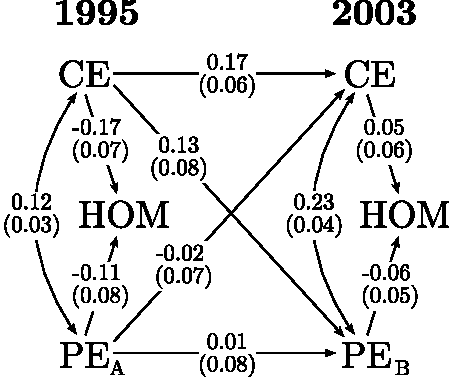
\includegraphics[width=0.5\linewidth]{./figure/ch3/crosslag_model_results_hom} }\subfloat[Victimization\label{fig:crosslagresults-2}]{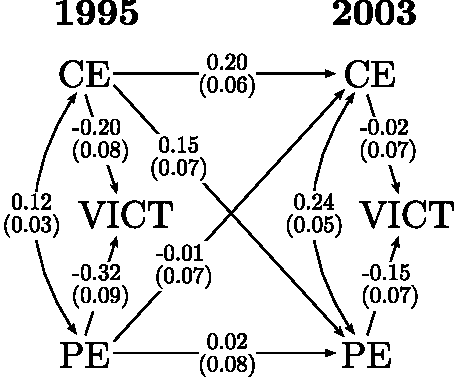
\includegraphics[width=0.5\linewidth]{./figure/ch3/crosslag_model_results_vict} }

}

\caption{Estimates from cross-lagged panel models of collective efficacy, police efficacy, and police-reported homicide (a) or survey-reported victimization (b).}\label{fig:crosslagresults}
\end{figure}
These models exhibit relatively good fit, though better for victimization than homicide. The homicide model's Satorra-Bentler scaled Chi-square is significant (\(p <.00\), \(\chi^{2} = 92.42\), \(df = 37\)) indicating overidentification restrictions in the model may not hold. Chi-square values increase in proportion to sample size, so rejection is common in even moderately-sized samples (Bollen 1989). Fit indices which adjust for sample size and/or model complexity provide better metrics for evaluating fit. The homicide model displays a Standardized Root Mean Square Residual (SRMR) of 0.020, Root Mean Square Error of Approximation (RMSEA) of 0.066 (90\% CI: 0.049, 0.084), and Tucker-Lewis Index (TLI) of 0.934. Typical values indicating good fit are an SRMR below 0.080, RMSEA close to or below 0.060, and TLI close to or above 0.950 (Hu and Bentler 1999). The victimization model displays a significant Chi-square (\(p = 0.03\), \(\chi^{2} = 55.14\), \(df = 37\)), an RMSEA of 0.038 (90\% CI: 0.12, 0.058), SRMR of 0.018, and TLI of 0.971.

\hypertarget{instrumental-variables-models}{%
\subsubsection{Instrumental Variables Models}\label{instrumental-variables-models}}

Cross-lagged models estimate the effects of collective efficacy and police efficacy on each over a relatively long span of time. Those models do not estimate their immediate effects on one-another, though they are permitted to exist with a contemporaneous error covariance at each time period. It is possible, however, that collective efficacy and police efficacy function as a sort of causal chain in a short time span. This section augments the cross-lagged model with instrumental variables to test the direct effect of collective efficacy on police efficacy in the short term while adjusting for the possibility of a reciprocal effect in the opposite direction.

Identifying causal effects in the presence of reciprocal feedback requires instrumental variables---variables which are relatively strongly correlated with the treatment of interest but impact the outcome only via the treatment or included covariates. With cross-sectional data, researchers typically use theory to locate and justify instruments. Sampson and Raudenbush (1999), for example, used attachment to neighborhood, friendship and kinship ties, and neighboring behavior as instruments for the effect of collective efficacy on crime and disorder, based on the assumption they would only impact crime and disorder via collective efficacy. In the present case, we are interested in the effects of collective efficacy and police efficacy on one-another. I am aware of no available instruments for police efficacy which are plausibly independent of collective efficacy.

When repeated observations are available, researchers may instead turn to lags of the endogenous variables as instruments under the assumption there are no cross-lagged effects---the instrument must be valid. A requirement of this approach, however, is that there is a strong association between observations of the same variable over time---the instrument must be relevant. Results of the prior section indicate a cross-lagged effect of collective efficacy on police efficacy and a strong intertemporal association within collective efficacy. If this cross-lagged effect is actually zero in the population and reflects only a true contemporaneous association, the instrument may be relevant and valid. Police efficacy does not, however, display any significant intertemporal relationship with itself. This means past police efficacy is unsuitable for use as an instrument for present police efficacy (Wooldridge 2003:493).

Consequently, lacking any valid or relevant instruments for police efficacy, estimation of simultaneous causal effects is limited to a unidirectional instrumental variables model of the effect of collective efficacy on police efficacy. I instrument the effect of collective efficacy on police efficacy using neighboring behavior in 1995, and both neighboring behavior and past collective efficacy in 2003. This cannot, of course, rule out the possibility that there is a contemporaneous effect of police efficacy on collective efficacy, but it provides evidence against assumptions that collective efficacy is purely descended from police efficacy. Because our focus here is only on the effect of collective efficacy on police efficacy, I do not model homicide or victimization as outcomes. Rather, lagged homicide is included to block potential cross-lagged effects from collective efficacy to police efficacy, though this may attenuate the relationship between collective efficacy across waves. Results are insensitive to excluding homicide. As before, police efficacy and collective efficacy in each time period are modeled as dependent on the structural neighborhood measures. Figure \ref{fig:ivmodel} depicts the full instrumental variable model.
\begin{figure}

{\centering 
\includegraphics[width=0.6\linewidth]{./figure/ch3/iv_model} 

}

\caption{Two-period instrumental variable model of police efficacy and collective efficacy.}\label{fig:ivmodel}
\end{figure}
I include attachment to the neighborhood in the equations for the first wave to block potential paths from neighboring behavior to police efficacy via attachment. Silver and Miller (2004:573--74) noted the possibility that attachment may be descended from collective efficacy if residents become more attached to their neighborhood when they perceive their neighbors to be committed to regulating deviance. In this specification, even if neighboring or police efficacy impact attachment, the path from collective efficacy to police efficacy is identified. The estimated effects of collective efficacy on police efficacy are robust to the omission of attachment in the first wave. Attachment is not available in the 2003 wave. It is possible this may compromise the validity of the neighboring behavior instrument by opening backdoor path to police efficacy. An auxiliary model using only 1995 collective efficacy as an instrument for 2003 collective efficacy produces similar results though with less precision.
\begin{figure}

{\centering 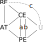
\includegraphics[width=0.4\linewidth]{./figure/ch3/nr_dag} 

}

\caption{Directed graph of reciprocal relationship between collective efficacy and police efficacy with neighboring behavior and attachment.}\label{fig:nrdag}
\end{figure}
An additional illustration may clarify assumptions in the model. If we consider only the equations for the first wave of the instrumental variables model and simplify to the relevant elements of the model, we arrive at the directed cyclic graph in Figure \ref{fig:nrdag}. Our interest is in path a from collective efficacy to police efficacy. Estimation of this is complicated because the reverse causal path, b, may exist, and there may also be omitted variables, U, confounding estimation of these pathways. While depicted as a confounder here, the causal role of attachment (AT) is also ambiguous. It may precede both collective efficacy and police efficacy as shown, or, perhaps it precedes collective efficacy but is descended from police efficacy. Similarly, it may either precede or be preceded by neighboring behavior (NE). Regardless of which case is true, path a is still identified using neighboring behavior as an instrument, under the assumption neighboring has no impact on police efficacy or its unmeasured antecedents net of included variables (i.e.~path \(c\) is zero).

Using past collective efficacy and police efficacy as instruments makes the strong assumption that the cross-lagged effects seen in the prior section are actually zero conditional on their contemporaneous reciprocal effects. Fortunately, the neighboring behavior instruments for collective efficacy are sufficient to identify the contemporaneous reciprocal effects while relaxing the restrictions on the cross-lagged effects. I found support for the restricted specification: Conditional on the associations in 2003, there are no substantively or statistically significant cross-lagged effects, and a Chi-square test between the restricted and unrestricted models is not significant. Note that this is not a test of the exclusion restriction for use of 1995 collective efficacy as an instrument for the effect of 2003 collective efficacy on police efficacy. In the presence of a reciprocal effect or confounding between collective efficacy and police efficacy in 2003, the cross-lagged path from 1995 collective efficacy to 2003 police efficacy is not identified. This test merely indicates the results do not rely on making the assumption of an absence of cross-lagged effects.

\hypertarget{instrumental-variables-model-results}{%
\subsubsection{Instrumental variables model results}\label{instrumental-variables-model-results}}

Figure \ref{fig:ivresults} displays selected results from the instrumental variables model. The key results seen here mirror those of the cross-lagged models in the prior section: Collective efficacy has a strong effect on police efficacy. As before, police efficacy displays no significant intertemporal relationship with itself conditional on collective efficacy and neighborhood sociodemographic structure. In contrast, collective efficacy exhibits inherent stability over time. These results provide evidence for the hypothesis that collective efficacy precedes police efficacy. Further, this suggests models which attempt to estimate the effect of collective efficacy on crime may be misspecified if they include police efficacy without estimating the indirect (mediated) effect of collective efficacy via police efficacy. This model cannot, however, rule out the existence of a simultaneous reciprocal path from police efficacy back to collective efficacy. The residual covariance between police efficacy and collective efficacy in both time periods is, however, substantively and statistically weak. Overall, this model fits well. Its Satorra-Bentler Chi-square is significant (\(p =.011\), \(\chi^{2}=42.70\), \(df = 24\)) but it displays a RMSEA of 0.048 (90\% CI: 0.023, 0.071), SRMR of 0.012, and TLI of 0.978.
\begin{figure}

{\centering 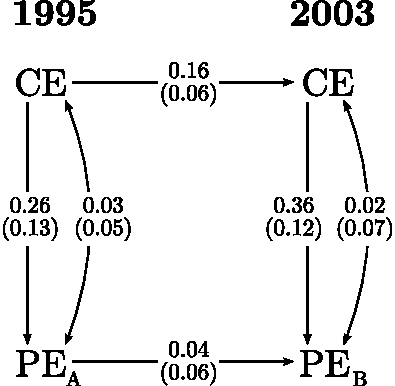
\includegraphics[width=0.6\linewidth]{./figure/ch3/iv_model_results} 

}

\caption{Estimates from instrumental variables panel model of the contemporaneous effect of collective efficacy on police efficacy.}\label{fig:ivresults}
\end{figure}
\hypertarget{discussion-1}{%
\section{Discussion}\label{discussion-1}}

The goal of this chapter is to evaluate the effects of collective efficacy and police efficacy on each other and on crime. Based on my own theoretical framework and the existing literature, I proposed two hypotheses: (1) collective efficacy and police efficacy have an interactive (moderated) effect on crime, and (2) collective efficacy and police efficacy are links in a causal chain. With regard to the first hypothesis, results from random- and fixed-effects panel models produce weak evidence for the moderation hypothesis. Estimates for the interaction terms are positive for perceived violence, victimization, and violent crime, but negative for homicide. In most cases these estimates not statistically distinguishable from zero, though the conservative fixed effects estimator indicates a positive effect for victimization and violent crime.

The weak evidence for moderation may in part be the result of the unexpectedly weak effects of collective efficacy in the 2003 period, which are at odds with much of the research in this area (Lanfear, Matsueda, and Beach 2020). The cause of this difference from the canonical 1995 results is unknown, as the data were collected in the same city, using the same survey instruments, and relatively soon after the 1995 PHDCN-CS. It is not possible to discern if this is an artifact of measurement or sampling variability. For instance, the smaller sample size of the 2003 CCAHS results in less reliable estimates of collective efficacy and police efficacy, which may in turn attenuate their estimated effects on crime.

Differences across time periods may also reflect actual changes in Chicago, such as a shift away from reliance on informal control or an overall decrease in serious violence which reduces variation, and thus the strength of relationships. It may also indicate some omitted factors outside both collective efficacy and police efficacy became more consequential in the later period. Local organizations, such as non-profits focused on community-building, have been suggested as an underappreciated source of crime control effects (Sharkey, Torrats-Espinosa, and Takyar 2017), but research in this area implies these effects should operate through collective efficacy (Morenoff, Sampson, and Raudenbush 2001). More longitudinal neighborhood studies of collective efficacy are warranted, particularly with additional waves of existing datasets, and researchers should be attentive to the possibility that effects vary across time periods. Both quantitative and qualitative research designs should also be used to investigate the possibility that means or effects of neighborhood social control are shifting over time.

With regard to Hypothesis 2, in contrast to the causal order assumed in some prior research---sometimes using the same data as this analysis---police efficacy appears to be descended from collective efficacy. Police efficacy exerts no statistically significant influence on collective efficacy over the eight-year gap between panels in cross-lagged models. In both cross-lagged models of intertemporal effects and instrumental variables models of immediate effects, collective efficacy exerts a strong effect on police efficacy. Further, police efficacy does not appear to have any intrinsic stability over time independent of collective efficacy and neighborhood structure. Future studies of neighborhood social control should carefully consider how models may be sensitive to assumptions about causal ordering. If police efficacy is causally descended from collective efficacy, research on collective efficacy and crime which controls for perceptions of police effectiveness and legitimacy may be inadvertently controlling for a post-treatment mediator, attenuating effects of collective efficacy on crime. This means results in which police efficacy appears to attenuate or dominate collective efficacy's effects on crime---as seen in the random- and fixed-effects models---may be misleading. Similarly, models featuring perceptions of police as a predictor of collective efficacy may be misspecified.

This causal ordering is plausible if most policing is reactive and collective efficacy captures in part the propensity of neighborhood residents to engage in monitoring and reporting of crime. This may result in more effective policing. An important implication of this, however, is that if exogenous factors depress perceived effectiveness and legitimacy of the police, it may result in higher crime overall by disrupting one of the pathways linking collective efficacy to crime. Police bias and misconduct, for instance, may reduce willingness to call police due to concerns over the potential consequences of calling. Perceptions of these consequences are important given how often that potential is realized as a fatal outcome, particularly for black subjects (Edwards, Esposito, and Lee 2018). For example, evidence indicates favorability toward police decreased precipitously across the United States following the murder of George Floyd by police officers in May 2020 and the resulting nationwide protests (Reny and Newman Forthcoming). In this way police bias and misconduct may undermine crime control functions of law enforcement. This is not a novel conclusion, but rather a small addition to the expansive literature drawing similar conclusions from different approaches and bases of evidence (National Research Council 2004; e.g., Tyler and Huo 2002; Wood, Tyler, and Papachristos 2020).

Future research should attempt to replicate the finding that collective efficacy precedes perceptions of police effectiveness and legitimacy, as well as investigate mechanisms for this relationship. Testing this effect convincingly is challenging as collective efficacy is difficult to manipulate experimentally and studies based on observational data---such as this one---rely on strong modeling assumptions. If this finding is robust, however, it may have an important implication for policy: interventions which increase police effectiveness and legitimacy may not increase collective efficacy---or perhaps may do so only indirectly via effects on crime and other neighborhood conditions. Regardless, of course, increasing the effectiveness and, in particular, fairness of policing would remain an important goals for both intrinsic reasons and reductions in crime and the harmful consequences of police-citizen encounters.

While beyond the scope of the present work, police efficacy may also affect the types of incidents in which residents will intervene and the form those interventions will take. For example, if residents believe police are highly effective but informal control is unlikely to be effective, they may invoke law enforcement to resolve minor incidents they would otherwise ignore or respond to informally (e.g. Schneider, Burcart, and Wilson 1976). This may be the case in neighborhoods with high police efficacy but weak informal social control, such as gentrifying neighborhoods with destabilized ties, as suggested by Kreager, Lyons, and Hays (2011:635) and (Lanfear, Beach, and Thomas 2018). Similarly, when calling the police is perceived as an inappropriate intervention for a situation---due to the possibility for violence or legal consequences---the ability to invoke other actors may affect both the decision to intervene and the ultimate outcome of interventions. Alternatives to invoking police, like community responder models, might reduce the relevance of police efficacy for disorder and crime control while improving outcomes for contacted individuals, particularly in terms of safety (Irwin and Pearl 2020). Future studies should examine how collective efficacy, police efficacy, and alternate means of intervention relate to both the type of situations in which residents intervene and the means by which they make those interventions.

In summary, this work attempts to identify how police efficacy---resident perceptions of police effectiveness and legitimacy---relates to collective efficacy and neighborhood crime rates. I examined first whether collective efficacy and police efficacy increase the effects of one-another on crime using longitudinal data in with variety of model specifications and estimators. I find weak evidence for a positive interaction. I then used cross-lagged panel models and instrumental variables to attempt to determine how police efficacy and collective efficacy are causally related. My results consistently indicate police efficacy is descended from collective efficacy, in contrast to a prominent literature that assumes the opposite causal relationship, that police efficacy promotes collective efficacy. This has important implications for future research as well as policy. Studies that treat collective efficacy as a mediator for police efficacy may produce biased and misleading estimates. Similarly, interventions that attempt to bolster collective efficacy by promoting perceptions of police efficacy may be unlikely to yield the intended results.

\hypertarget{conclusion}{%
\chapter*{Conclusion}\label{conclusion}}
\addcontentsline{toc}{chapter}{Conclusion}

If we don't want Conclusion to have a chapter number next to it, we can add the \texttt{\{-\}} attribute.

\textbf{More info}

And here's some other random info: the first paragraph after a chapter title or section head \emph{shouldn't be} indented, because indents are to tell the reader that you're starting a new paragraph. Since that's obvious after a chapter or section title, proper typesetting doesn't add an indent there.

\appendix

\hypertarget{measures}{%
\chapter{Data and Measurement Overview}\label{measures}}

This appendix provides an overview of all data used in this dissertation as well as approaches used to derive composite measures from indicators (e.g., multilevel measurement models).

\hypertarget{neighborhood-structural-measures}{%
\section{Neighborhood Structural Measures}\label{neighborhood-structural-measures}}

The social disorganization tradition recognizes crime and social control are rooted in structural characteristics of neighborhoods. To construct these measures, I obtained nine decennial census measures from the Longitudinal Tract Data Base (LTDB) (Logan, Xu, and Stults 2014) based on those used by Sampson, Raudenbush, and Earls (1997). The LTDB reweights indicators across changing boundaries between the 1990 and 2000 censuses to ensure they describe the same geographic areas. All measures are percentages and are listed in \ref{tab:structurefactors}. I use an oblimin-rotated alpha-scoring factor analysis to perform dimension reduction on these measures (Kaiser and Caffrey 1965). The factors were calculated simultaneously using both 1990 and 2001 observations for each NC to generate comparable measures over time. Three factors explain 87\% of variation in the nine indicators and exhibit acceptable model fit (\(\chi^{2}=7.69\), \(df = 12\), \(p=0.81\)). Loadings are depicted in \ref{tab:structurefactors}.

\providecommand{\docline}[3]{\noalign{\global\setlength{\arrayrulewidth}{#1}}\arrayrulecolor[HTML]{#2}\cline{#3}}

\setlength{\tabcolsep}{4pt}

\renewcommand*{\arraystretch}{0.8}
\begin{longtable}[c]{|p{2.00in}|p{1.20in}|p{1.20in}|p{1.20in}}

\caption{\label{tab:structurefactors} Factor Loadings for Neighborhood Structural Measures}\label{tab:unnamed-chunk-5}\\

\hhline{>{\arrayrulecolor[HTML]{000000}\global\arrayrulewidth=1pt}->{\arrayrulecolor[HTML]{000000}\global\arrayrulewidth=1pt}->{\arrayrulecolor[HTML]{000000}\global\arrayrulewidth=1pt}->{\arrayrulecolor[HTML]{000000}\global\arrayrulewidth=1pt}-}

\multicolumn{1}{!{\color[HTML]{000000}\vrule width 0pt}>{\raggedright}p{\dimexpr 2in+0\tabcolsep+0\arrayrulewidth}}{\fontsize{11}{11}\selectfont{\textcolor[HTML]{000000}{\global\setmainfont{Latin Modern Roman}Measure}}} & \multicolumn{1}{!{\color[HTML]{000000}\vrule width 0pt}>{\centering}p{\dimexpr 1.2in+0\tabcolsep+0\arrayrulewidth}}{\fontsize{11}{11}\selectfont{\textcolor[HTML]{000000}{\global\setmainfont{Latin Modern Roman}Disadvantage}}} & \multicolumn{1}{!{\color[HTML]{000000}\vrule width 0pt}>{\centering}p{\dimexpr 1.2in+0\tabcolsep+0\arrayrulewidth}}{\fontsize{11}{11}\selectfont{\textcolor[HTML]{000000}{\global\setmainfont{Latin Modern Roman}Hispanic / Immigration}}} & \multicolumn{1}{!{\color[HTML]{000000}\vrule width 0pt}>{\centering}p{\dimexpr 1.2in+0\tabcolsep+0\arrayrulewidth}!{\color[HTML]{000000}\vrule width 0pt}}{\fontsize{11}{11}\selectfont{\textcolor[HTML]{000000}{\global\setmainfont{Latin Modern Roman}Stability}}} \\

\noalign{\global\setlength{\arrayrulewidth}{0.5pt}}\arrayrulecolor[HTML]{000000}\cline{1-4}

\endfirsthead

\hhline{>{\arrayrulecolor[HTML]{000000}\global\arrayrulewidth=1pt}->{\arrayrulecolor[HTML]{000000}\global\arrayrulewidth=1pt}->{\arrayrulecolor[HTML]{000000}\global\arrayrulewidth=1pt}->{\arrayrulecolor[HTML]{000000}\global\arrayrulewidth=1pt}-}

\multicolumn{1}{!{\color[HTML]{000000}\vrule width 0pt}>{\raggedright}p{\dimexpr 2in+0\tabcolsep+0\arrayrulewidth}}{\fontsize{11}{11}\selectfont{\textcolor[HTML]{000000}{\global\setmainfont{Latin Modern Roman}Measure}}} & \multicolumn{1}{!{\color[HTML]{000000}\vrule width 0pt}>{\centering}p{\dimexpr 1.2in+0\tabcolsep+0\arrayrulewidth}}{\fontsize{11}{11}\selectfont{\textcolor[HTML]{000000}{\global\setmainfont{Latin Modern Roman}Disadvantage}}} & \multicolumn{1}{!{\color[HTML]{000000}\vrule width 0pt}>{\centering}p{\dimexpr 1.2in+0\tabcolsep+0\arrayrulewidth}}{\fontsize{11}{11}\selectfont{\textcolor[HTML]{000000}{\global\setmainfont{Latin Modern Roman}Hispanic / Immigration}}} & \multicolumn{1}{!{\color[HTML]{000000}\vrule width 0pt}>{\centering}p{\dimexpr 1.2in+0\tabcolsep+0\arrayrulewidth}!{\color[HTML]{000000}\vrule width 0pt}}{\fontsize{11}{11}\selectfont{\textcolor[HTML]{000000}{\global\setmainfont{Latin Modern Roman}Stability}}} \\

\noalign{\global\setlength{\arrayrulewidth}{0.5pt}}\arrayrulecolor[HTML]{000000}\cline{1-4}\endhead



\multicolumn{1}{!{\color[HTML]{FFFFFF}\vrule width 0pt}>{\raggedright}p{\dimexpr 2in+0\tabcolsep+0\arrayrulewidth}}{\fontsize{11}{11}\selectfont{\textcolor[HTML]{000000}{\global\setmainfont{Latin Modern Roman}Eigenvalue}}} & \multicolumn{1}{!{\color[HTML]{FFFFFF}\vrule width 0pt}>{\centering}p{\dimexpr 1.2in+0\tabcolsep+0\arrayrulewidth}}{\fontsize{11}{11}\selectfont{\textcolor[HTML]{000000}{\global\setmainfont{Latin Modern Roman}3.15}}} & \multicolumn{1}{!{\color[HTML]{FFFFFF}\vrule width 0pt}>{\centering}p{\dimexpr 1.2in+0\tabcolsep+0\arrayrulewidth}}{\fontsize{11}{11}\selectfont{\textcolor[HTML]{000000}{\global\setmainfont{Latin Modern Roman}2.74}}} & \multicolumn{1}{!{\color[HTML]{FFFFFF}\vrule width 0pt}>{\centering}p{\dimexpr 1.2in+0\tabcolsep+0\arrayrulewidth}!{\color[HTML]{FFFFFF}\vrule width 0pt}}{\fontsize{11}{11}\selectfont{\textcolor[HTML]{000000}{\global\setmainfont{Latin Modern Roman}1.98}}} \\





\multicolumn{1}{!{\color[HTML]{FFFFFF}\vrule width 0pt}>{\raggedright}p{\dimexpr 2in+0\tabcolsep+0\arrayrulewidth}}{\fontsize{11}{11}\selectfont{\textcolor[HTML]{000000}{\global\setmainfont{Latin Modern Roman}Proportion of Variance Explained}}} & \multicolumn{1}{!{\color[HTML]{FFFFFF}\vrule width 0pt}>{\centering}p{\dimexpr 1.2in+0\tabcolsep+0\arrayrulewidth}}{\fontsize{11}{11}\selectfont{\textcolor[HTML]{000000}{\global\setmainfont{Latin Modern Roman}0.35}}} & \multicolumn{1}{!{\color[HTML]{FFFFFF}\vrule width 0pt}>{\centering}p{\dimexpr 1.2in+0\tabcolsep+0\arrayrulewidth}}{\fontsize{11}{11}\selectfont{\textcolor[HTML]{000000}{\global\setmainfont{Latin Modern Roman}0.3}}} & \multicolumn{1}{!{\color[HTML]{FFFFFF}\vrule width 0pt}>{\centering}p{\dimexpr 1.2in+0\tabcolsep+0\arrayrulewidth}!{\color[HTML]{FFFFFF}\vrule width 0pt}}{\fontsize{11}{11}\selectfont{\textcolor[HTML]{000000}{\global\setmainfont{Latin Modern Roman}0.22}}} \\

\noalign{\global\setlength{\arrayrulewidth}{1pt}}\arrayrulecolor[HTML]{000000}\cline{1-4}\endfoot



\multicolumn{1}{!{\color[HTML]{000000}\vrule width 0pt}>{\raggedright}p{\dimexpr 2in+0\tabcolsep+0\arrayrulewidth}}{\fontsize{11}{11}\selectfont{\textcolor[HTML]{000000}{\global\setmainfont{Latin Modern Roman}Under 18}}} & \multicolumn{1}{!{\color[HTML]{000000}\vrule width 0pt}>{\centering}p{\dimexpr 1.2in+0\tabcolsep+0\arrayrulewidth}}{\fontsize{11}{11}\selectfont{\textcolor[HTML]{000000}{\global\setmainfont{Latin Modern Roman}1.03}}} & \multicolumn{1}{!{\color[HTML]{000000}\vrule width 0pt}>{\centering}p{\dimexpr 1.2in+0\tabcolsep+0\arrayrulewidth}}{\fontsize{11}{11}\selectfont{\textcolor[HTML]{000000}{\global\setmainfont{Latin Modern Roman}0.25}}} & \multicolumn{1}{!{\color[HTML]{000000}\vrule width 0pt}>{\centering}p{\dimexpr 1.2in+0\tabcolsep+0\arrayrulewidth}!{\color[HTML]{000000}\vrule width 0pt}}{\fontsize{11}{11}\selectfont{\textcolor[HTML]{000000}{\global\setmainfont{Latin Modern Roman}-0.13}}} \\





\multicolumn{1}{!{\color[HTML]{000000}\vrule width 0pt}>{\raggedright}p{\dimexpr 2in+0\tabcolsep+0\arrayrulewidth}}{\fontsize{11}{11}\selectfont{\textcolor[HTML]{000000}{\global\setmainfont{Latin Modern Roman}Unemployment}}} & \multicolumn{1}{!{\color[HTML]{000000}\vrule width 0pt}>{\centering}p{\dimexpr 1.2in+0\tabcolsep+0\arrayrulewidth}}{\fontsize{11}{11}\selectfont{\textcolor[HTML]{000000}{\global\setmainfont{Latin Modern Roman}0.74}}} & \multicolumn{1}{!{\color[HTML]{000000}\vrule width 0pt}>{\centering}p{\dimexpr 1.2in+0\tabcolsep+0\arrayrulewidth}}{\fontsize{11}{11}\selectfont{\textcolor[HTML]{000000}{\global\setmainfont{Latin Modern Roman}-0.33}}} & \multicolumn{1}{!{\color[HTML]{000000}\vrule width 0pt}>{\centering}p{\dimexpr 1.2in+0\tabcolsep+0\arrayrulewidth}!{\color[HTML]{000000}\vrule width 0pt}}{\fontsize{11}{11}\selectfont{\textcolor[HTML]{000000}{\global\setmainfont{Latin Modern Roman}0.14}}} \\





\multicolumn{1}{!{\color[HTML]{000000}\vrule width 0pt}>{\raggedright}p{\dimexpr 2in+0\tabcolsep+0\arrayrulewidth}}{\fontsize{11}{11}\selectfont{\textcolor[HTML]{000000}{\global\setmainfont{Latin Modern Roman}Poverty}}} & \multicolumn{1}{!{\color[HTML]{000000}\vrule width 0pt}>{\centering}p{\dimexpr 1.2in+0\tabcolsep+0\arrayrulewidth}}{\fontsize{11}{11}\selectfont{\textcolor[HTML]{000000}{\global\setmainfont{Latin Modern Roman}0.69}}} & \multicolumn{1}{!{\color[HTML]{000000}\vrule width 0pt}>{\centering}p{\dimexpr 1.2in+0\tabcolsep+0\arrayrulewidth}}{\fontsize{11}{11}\selectfont{\textcolor[HTML]{000000}{\global\setmainfont{Latin Modern Roman}-0.15}}} & \multicolumn{1}{!{\color[HTML]{000000}\vrule width 0pt}>{\centering}p{\dimexpr 1.2in+0\tabcolsep+0\arrayrulewidth}!{\color[HTML]{000000}\vrule width 0pt}}{\fontsize{11}{11}\selectfont{\textcolor[HTML]{000000}{\global\setmainfont{Latin Modern Roman}0.43}}} \\





\multicolumn{1}{!{\color[HTML]{000000}\vrule width 0pt}>{\raggedright}p{\dimexpr 2in+0\tabcolsep+0\arrayrulewidth}}{\fontsize{11}{11}\selectfont{\textcolor[HTML]{000000}{\global\setmainfont{Latin Modern Roman}Female-Headed Households}}} & \multicolumn{1}{!{\color[HTML]{000000}\vrule width 0pt}>{\centering}p{\dimexpr 1.2in+0\tabcolsep+0\arrayrulewidth}}{\fontsize{11}{11}\selectfont{\textcolor[HTML]{000000}{\global\setmainfont{Latin Modern Roman}0.67}}} & \multicolumn{1}{!{\color[HTML]{000000}\vrule width 0pt}>{\centering}p{\dimexpr 1.2in+0\tabcolsep+0\arrayrulewidth}}{\fontsize{11}{11}\selectfont{\textcolor[HTML]{000000}{\global\setmainfont{Latin Modern Roman}-0.44}}} & \multicolumn{1}{!{\color[HTML]{000000}\vrule width 0pt}>{\centering}p{\dimexpr 1.2in+0\tabcolsep+0\arrayrulewidth}!{\color[HTML]{000000}\vrule width 0pt}}{\fontsize{11}{11}\selectfont{\textcolor[HTML]{000000}{\global\setmainfont{Latin Modern Roman}0.27}}} \\





\multicolumn{1}{!{\color[HTML]{000000}\vrule width 0pt}>{\raggedright}p{\dimexpr 2in+0\tabcolsep+0\arrayrulewidth}}{\fontsize{11}{11}\selectfont{\textcolor[HTML]{000000}{\global\setmainfont{Latin Modern Roman}Home Ownership}}} & \multicolumn{1}{!{\color[HTML]{000000}\vrule width 0pt}>{\centering}p{\dimexpr 1.2in+0\tabcolsep+0\arrayrulewidth}}{\fontsize{11}{11}\selectfont{\textcolor[HTML]{000000}{\global\setmainfont{Latin Modern Roman}-0.09}}} & \multicolumn{1}{!{\color[HTML]{000000}\vrule width 0pt}>{\centering}p{\dimexpr 1.2in+0\tabcolsep+0\arrayrulewidth}}{\fontsize{11}{11}\selectfont{\textcolor[HTML]{000000}{\global\setmainfont{Latin Modern Roman}0.02}}} & \multicolumn{1}{!{\color[HTML]{000000}\vrule width 0pt}>{\centering}p{\dimexpr 1.2in+0\tabcolsep+0\arrayrulewidth}!{\color[HTML]{000000}\vrule width 0pt}}{\fontsize{11}{11}\selectfont{\textcolor[HTML]{000000}{\global\setmainfont{Latin Modern Roman}-0.96}}} \\





\multicolumn{1}{!{\color[HTML]{000000}\vrule width 0pt}>{\raggedright}p{\dimexpr 2in+0\tabcolsep+0\arrayrulewidth}}{\fontsize{11}{11}\selectfont{\textcolor[HTML]{000000}{\global\setmainfont{Latin Modern Roman}Moved in Last 10 Years}}} & \multicolumn{1}{!{\color[HTML]{000000}\vrule width 0pt}>{\centering}p{\dimexpr 1.2in+0\tabcolsep+0\arrayrulewidth}}{\fontsize{11}{11}\selectfont{\textcolor[HTML]{000000}{\global\setmainfont{Latin Modern Roman}-0.19}}} & \multicolumn{1}{!{\color[HTML]{000000}\vrule width 0pt}>{\centering}p{\dimexpr 1.2in+0\tabcolsep+0\arrayrulewidth}}{\fontsize{11}{11}\selectfont{\textcolor[HTML]{000000}{\global\setmainfont{Latin Modern Roman}0.34}}} & \multicolumn{1}{!{\color[HTML]{000000}\vrule width 0pt}>{\centering}p{\dimexpr 1.2in+0\tabcolsep+0\arrayrulewidth}!{\color[HTML]{000000}\vrule width 0pt}}{\fontsize{11}{11}\selectfont{\textcolor[HTML]{000000}{\global\setmainfont{Latin Modern Roman}0.79}}} \\





\multicolumn{1}{!{\color[HTML]{000000}\vrule width 0pt}>{\raggedright}p{\dimexpr 2in+0\tabcolsep+0\arrayrulewidth}}{\fontsize{11}{11}\selectfont{\textcolor[HTML]{000000}{\global\setmainfont{Latin Modern Roman}Hispanic}}} & \multicolumn{1}{!{\color[HTML]{000000}\vrule width 0pt}>{\centering}p{\dimexpr 1.2in+0\tabcolsep+0\arrayrulewidth}}{\fontsize{11}{11}\selectfont{\textcolor[HTML]{000000}{\global\setmainfont{Latin Modern Roman}0.30}}} & \multicolumn{1}{!{\color[HTML]{000000}\vrule width 0pt}>{\centering}p{\dimexpr 1.2in+0\tabcolsep+0\arrayrulewidth}}{\fontsize{11}{11}\selectfont{\textcolor[HTML]{000000}{\global\setmainfont{Latin Modern Roman}0.93}}} & \multicolumn{1}{!{\color[HTML]{000000}\vrule width 0pt}>{\centering}p{\dimexpr 1.2in+0\tabcolsep+0\arrayrulewidth}!{\color[HTML]{000000}\vrule width 0pt}}{\fontsize{11}{11}\selectfont{\textcolor[HTML]{000000}{\global\setmainfont{Latin Modern Roman}0.05}}} \\





\multicolumn{1}{!{\color[HTML]{000000}\vrule width 0pt}>{\raggedright}p{\dimexpr 2in+0\tabcolsep+0\arrayrulewidth}}{\fontsize{11}{11}\selectfont{\textcolor[HTML]{000000}{\global\setmainfont{Latin Modern Roman}Foreign Born}}} & \multicolumn{1}{!{\color[HTML]{000000}\vrule width 0pt}>{\centering}p{\dimexpr 1.2in+0\tabcolsep+0\arrayrulewidth}}{\fontsize{11}{11}\selectfont{\textcolor[HTML]{000000}{\global\setmainfont{Latin Modern Roman}-0.12}}} & \multicolumn{1}{!{\color[HTML]{000000}\vrule width 0pt}>{\centering}p{\dimexpr 1.2in+0\tabcolsep+0\arrayrulewidth}}{\fontsize{11}{11}\selectfont{\textcolor[HTML]{000000}{\global\setmainfont{Latin Modern Roman}0.83}}} & \multicolumn{1}{!{\color[HTML]{000000}\vrule width 0pt}>{\centering}p{\dimexpr 1.2in+0\tabcolsep+0\arrayrulewidth}!{\color[HTML]{000000}\vrule width 0pt}}{\fontsize{11}{11}\selectfont{\textcolor[HTML]{000000}{\global\setmainfont{Latin Modern Roman}0.15}}} \\





\multicolumn{1}{!{\color[HTML]{000000}\vrule width 0pt}>{\raggedright}p{\dimexpr 2in+0\tabcolsep+0\arrayrulewidth}}{\fontsize{11}{11}\selectfont{\textcolor[HTML]{000000}{\global\setmainfont{Latin Modern Roman}Non-Hispanic Black}}} & \multicolumn{1}{!{\color[HTML]{000000}\vrule width 0pt}>{\centering}p{\dimexpr 1.2in+0\tabcolsep+0\arrayrulewidth}}{\fontsize{11}{11}\selectfont{\textcolor[HTML]{000000}{\global\setmainfont{Latin Modern Roman}0.43}}} & \multicolumn{1}{!{\color[HTML]{000000}\vrule width 0pt}>{\centering}p{\dimexpr 1.2in+0\tabcolsep+0\arrayrulewidth}}{\fontsize{11}{11}\selectfont{\textcolor[HTML]{000000}{\global\setmainfont{Latin Modern Roman}-0.71}}} & \multicolumn{1}{!{\color[HTML]{000000}\vrule width 0pt}>{\centering}p{\dimexpr 1.2in+0\tabcolsep+0\arrayrulewidth}!{\color[HTML]{000000}\vrule width 0pt}}{\fontsize{11}{11}\selectfont{\textcolor[HTML]{000000}{\global\setmainfont{Latin Modern Roman}-0.03}}} \\

\noalign{\global\setlength{\arrayrulewidth}{0.5pt}}\arrayrulecolor[HTML]{000000}\cline{1-4}

\end{longtable}
Based on the indicators which most highly load on each factor, they are described as disadvantage, Hispanic / immigrant, and stability. Disadvantage loads primarily on under-18 population, unemployment, poverty, and female-headed households, and to a lesser-degree non-Hispanic black population. Hispanic / immigrant loads on Hispanic population, foreign born, and negatively on non-Hispanic black. Stability loads negatively on home ownership and positively on moves in the last 10 years. These were extracted as neighborhood-level correlation-preserving factor scores to produce a parsimonious set of structural predictors for use in subsequent models (ten Berge et al. 1999).

While the measures were chosen to replicate the structural measures used in Sampson, Raudenbush, and Earls (1997), one indicator for disadvantage---percent of families on public assistance---was not available in the LTDB. The indicator for recent moves is also in the last 10 years rather than 5 years. Even with these differences---and calculating across both waves simultaneously---the resultant factor scores for 1990 neighborhoods are all correlated at over \(\rho=.95\) with those from Sampson, Raudenbush, and Earls (1997).\footnote{Another benefit of recalculating these factors is that the PHDCN-CS data has missing values on all neighborhood measures for one NC (749). Calculating new scores thus recovers one missing observation.}

\hypertarget{neighborhood-social-and-perceptual-measures}{%
\section{Neighborhood Social and Perceptual Measures}\label{neighborhood-social-and-perceptual-measures}}

The neighborhood social and perceptual measures were calculated using multi-level measurement models which adjust for sociodemographic composition of neighborhoods and conservatively shrink estimates toward zero where interrater reliability is lower (Sampson, Raudenbush, and Earls 1997). These measures include collective efficacy, police efficacy, perceived violence, legal cynicism, violent victimization, and local ties and exchange. Violent victimization is a single binary indicator estimated with a logistic regression while the remaining measures feature multiple four- or five-category ordinal indicators estimated using linear regression. Multiple-indicator measures include dummies for each indicator to adjust for item difficulty and random respondent intercepts. All models feature neighborhood-level random intercepts which are extracted and used as in subsequent models as empirical Bayes estimates of the neighborhood measures. I use a single factor for Collective Efficacy which combines Cohesion and Trust and Informal Control Expectations to mimic existing work in this field and using these data. A two-factor solution is preferred in confirmatory factor models, though the resulting separate factors are highly correlated at both the individual (\(\rho=0.70\) in 1995, \(\rho=0.67\) in 2003) and neighborhood level (\(\rho=0.71\) in 1995, \(\rho=0.64\) in 2003).\footnote{I could potentially fit alternate models using an interaction between the separate factors but it wouldn't give any leverage on any questions I am interested in.}

\ref{tab:structuremeasures} depicts all indicators used to calculate the neighborhood measures including loadings from confirmatory factor analyses and overall neighborhood-level measure reliability from each multilevel model. Bracketed loadings reflect loadings on separate Cohesion and Trust and Informal Control Expectations factors for comparison to the combined Collective Efficacy Factor. For measures with two indicators like friend and kinship ties, a polychoric correlation between the indicators is reported in parentheses instead of item loadings. Note some measures differ between the 1995 and 2003 surveys, in particular, the indicators for police efficacy. Dashes indicate missing indicators for a given survey.

\providecommand{\docline}[3]{\noalign{\global\setlength{\arrayrulewidth}{#1}}\arrayrulecolor[HTML]{#2}\cline{#3}}

\setlength{\tabcolsep}{4pt}

\renewcommand*{\arraystretch}{0.8}
\begin{longtable}[c]{|p{0.20in}|p{3.00in}|p{1.00in}|p{1.00in}}

\caption{\label{tab:structuremeasures} Loadings and Reliabilities for Neighborhood Perceptual Measures}\label{tab:unnamed-chunk-6}\\

\hhline{>{\arrayrulecolor[HTML]{000000}\global\arrayrulewidth=1pt}->{\arrayrulecolor[HTML]{000000}\global\arrayrulewidth=1pt}->{\arrayrulecolor[HTML]{000000}\global\arrayrulewidth=1pt}->{\arrayrulecolor[HTML]{000000}\global\arrayrulewidth=1pt}-}

\multicolumn{1}{!{\color[HTML]{FFFFFF}\vrule width 0pt}>{\raggedright}p{\dimexpr 0.2in+0\tabcolsep+0\arrayrulewidth}}{\fontsize{11}{11}\selectfont{\textcolor[HTML]{000000}{\global\setmainfont{Latin Modern Roman}}}} & \multicolumn{1}{!{\color[HTML]{FFFFFF}\vrule width 0pt}>{\raggedright}p{\dimexpr 3in+0\tabcolsep+0\arrayrulewidth}}{\fontsize{11}{11}\selectfont{\textcolor[HTML]{000000}{\global\setmainfont{Latin Modern Roman}}}} & \multicolumn{2}{!{\color[HTML]{FFFFFF}\vrule width 0pt}>{\centering}p{\dimexpr 2in+2\tabcolsep+1\arrayrulewidth}}{\fontsize{11}{11}\selectfont{\textcolor[HTML]{000000}{\global\setmainfont{Latin Modern Roman}Loadings / Reliabilites (A)}}} \\



\multicolumn{2}{!{\color[HTML]{000000}\vrule width 0pt}>{\raggedright}p{\dimexpr 3.2in+2\tabcolsep+1\arrayrulewidth}}{\fontsize{9}{9}\selectfont{\textcolor[HTML]{000000}{\global\setmainfont{Latin Modern Roman}Measure / Indicator}}} & \multicolumn{1}{!{\color[HTML]{000000}\vrule width 0pt}>{\centering}p{\dimexpr 1in+0\tabcolsep+0\arrayrulewidth}}{\fontsize{9}{9}\selectfont{\textcolor[HTML]{000000}{\global\setmainfont{Latin Modern Roman}PHDCN\linebreak (1995)}}} & \multicolumn{1}{!{\color[HTML]{000000}\vrule width 0pt}>{\centering}p{\dimexpr 1in+0\tabcolsep+0\arrayrulewidth}!{\color[HTML]{000000}\vrule width 0pt}}{\fontsize{9}{9}\selectfont{\textcolor[HTML]{000000}{\global\setmainfont{Latin Modern Roman}CCAHS\linebreak (2003)}}} \\

\noalign{\global\setlength{\arrayrulewidth}{0.5pt}}\arrayrulecolor[HTML]{000000}\cline{1-4}

\endfirsthead

\hhline{>{\arrayrulecolor[HTML]{000000}\global\arrayrulewidth=1pt}->{\arrayrulecolor[HTML]{000000}\global\arrayrulewidth=1pt}->{\arrayrulecolor[HTML]{000000}\global\arrayrulewidth=1pt}->{\arrayrulecolor[HTML]{000000}\global\arrayrulewidth=1pt}-}

\multicolumn{1}{!{\color[HTML]{FFFFFF}\vrule width 0pt}>{\raggedright}p{\dimexpr 0.2in+0\tabcolsep+0\arrayrulewidth}}{\fontsize{11}{11}\selectfont{\textcolor[HTML]{000000}{\global\setmainfont{Latin Modern Roman}}}} & \multicolumn{1}{!{\color[HTML]{FFFFFF}\vrule width 0pt}>{\raggedright}p{\dimexpr 3in+0\tabcolsep+0\arrayrulewidth}}{\fontsize{11}{11}\selectfont{\textcolor[HTML]{000000}{\global\setmainfont{Latin Modern Roman}}}} & \multicolumn{2}{!{\color[HTML]{FFFFFF}\vrule width 0pt}>{\centering}p{\dimexpr 2in+2\tabcolsep+1\arrayrulewidth}}{\fontsize{11}{11}\selectfont{\textcolor[HTML]{000000}{\global\setmainfont{Latin Modern Roman}Loadings / Reliabilites (A)}}} \\





\multicolumn{2}{!{\color[HTML]{000000}\vrule width 0pt}>{\raggedright}p{\dimexpr 3.2in+2\tabcolsep+1\arrayrulewidth}}{\fontsize{9}{9}\selectfont{\textcolor[HTML]{000000}{\global\setmainfont{Latin Modern Roman}Measure / Indicator}}} & \multicolumn{1}{!{\color[HTML]{000000}\vrule width 0pt}>{\centering}p{\dimexpr 1in+0\tabcolsep+0\arrayrulewidth}}{\fontsize{9}{9}\selectfont{\textcolor[HTML]{000000}{\global\setmainfont{Latin Modern Roman}PHDCN\linebreak (1995)}}} & \multicolumn{1}{!{\color[HTML]{000000}\vrule width 0pt}>{\centering}p{\dimexpr 1in+0\tabcolsep+0\arrayrulewidth}!{\color[HTML]{000000}\vrule width 0pt}}{\fontsize{9}{9}\selectfont{\textcolor[HTML]{000000}{\global\setmainfont{Latin Modern Roman}CCAHS\linebreak (2003)}}} \\

\noalign{\global\setlength{\arrayrulewidth}{0.5pt}}\arrayrulecolor[HTML]{000000}\cline{1-4}\endhead



\multicolumn{2}{!{\color[HTML]{000000}\vrule width 0pt}>{\raggedright}p{\dimexpr 3.2in+2\tabcolsep+1\arrayrulewidth}}{\fontsize{9}{9}\selectfont{\textcolor[HTML]{000000}{\global\setmainfont{Latin Modern Roman}Collective Efficacy (Cohesion \& Trust + Informal Control Expectations)}}} & \multicolumn{1}{!{\color[HTML]{000000}\vrule width 0pt}>{\centering}p{\dimexpr 1in+0\tabcolsep+0\arrayrulewidth}}{\fontsize{9}{9}\selectfont{\textcolor[HTML]{000000}{\global\setmainfont{Latin Modern Roman}A=0.758}}} & \multicolumn{1}{!{\color[HTML]{000000}\vrule width 0pt}>{\centering}p{\dimexpr 1in+0\tabcolsep+0\arrayrulewidth}!{\color[HTML]{000000}\vrule width 0pt}}{\fontsize{9}{9}\selectfont{\textcolor[HTML]{000000}{\global\setmainfont{Latin Modern Roman}A=0.503}}} \\





\multicolumn{2}{!{\color[HTML]{000000}\vrule width 0pt}>{\raggedright}p{\dimexpr 3.2in+2\tabcolsep+1\arrayrulewidth}}{\fontsize{9}{9}\selectfont{\textcolor[HTML]{000000}{\global\setmainfont{Latin Modern Roman}Cohesion \& Trust ("How much do you agree that…")}}} & \multicolumn{1}{!{\color[HTML]{000000}\vrule width 0pt}>{\centering}p{\dimexpr 1in+0\tabcolsep+0\arrayrulewidth}}{\fontsize{9}{9}\selectfont{\textcolor[HTML]{000000}{\global\setmainfont{Latin Modern Roman}A=0.763}}} & \multicolumn{1}{!{\color[HTML]{000000}\vrule width 0pt}>{\centering}p{\dimexpr 1in+0\tabcolsep+0\arrayrulewidth}!{\color[HTML]{000000}\vrule width 0pt}}{\fontsize{9}{9}\selectfont{\textcolor[HTML]{000000}{\global\setmainfont{Latin Modern Roman}A=0.453}}} \\





\multicolumn{1}{!{\color[HTML]{000000}\vrule width 0pt}>{\raggedright}p{\dimexpr 0.2in+0\tabcolsep+0\arrayrulewidth}}{\fontsize{9}{9}\selectfont{\textcolor[HTML]{000000}{\global\setmainfont{Latin Modern Roman}}}} & \multicolumn{1}{!{\color[HTML]{000000}\vrule width 0pt}>{\raggedright}p{\dimexpr 3in+0\tabcolsep+0\arrayrulewidth}}{\fontsize{9}{9}\selectfont{\textcolor[HTML]{000000}{\global\setmainfont{Latin Modern Roman}People around here are willing to help their neighbors.}}} & \multicolumn{1}{!{\color[HTML]{000000}\vrule width 0pt}>{\centering}p{\dimexpr 1in+0\tabcolsep+0\arrayrulewidth}}{\fontsize{9}{9}\selectfont{\textcolor[HTML]{000000}{\global\setmainfont{Latin Modern Roman}0.699 [0.766]}}} & \multicolumn{1}{!{\color[HTML]{000000}\vrule width 0pt}>{\centering}p{\dimexpr 1in+0\tabcolsep+0\arrayrulewidth}!{\color[HTML]{000000}\vrule width 0pt}}{\fontsize{9}{9}\selectfont{\textcolor[HTML]{000000}{\global\setmainfont{Latin Modern Roman}0.775 [0.813]}}} \\





\multicolumn{1}{!{\color[HTML]{000000}\vrule width 0pt}>{\raggedright}p{\dimexpr 0.2in+0\tabcolsep+0\arrayrulewidth}}{\fontsize{9}{9}\selectfont{\textcolor[HTML]{000000}{\global\setmainfont{Latin Modern Roman}}}} & \multicolumn{1}{!{\color[HTML]{000000}\vrule width 0pt}>{\raggedright}p{\dimexpr 3in+0\tabcolsep+0\arrayrulewidth}}{\fontsize{9}{9}\selectfont{\textcolor[HTML]{000000}{\global\setmainfont{Latin Modern Roman}People in this neighborhood can be trusted.}}} & \multicolumn{1}{!{\color[HTML]{000000}\vrule width 0pt}>{\centering}p{\dimexpr 1in+0\tabcolsep+0\arrayrulewidth}}{\fontsize{9}{9}\selectfont{\textcolor[HTML]{000000}{\global\setmainfont{Latin Modern Roman}0.726 [0.795]}}} & \multicolumn{1}{!{\color[HTML]{000000}\vrule width 0pt}>{\centering}p{\dimexpr 1in+0\tabcolsep+0\arrayrulewidth}!{\color[HTML]{000000}\vrule width 0pt}}{\fontsize{9}{9}\selectfont{\textcolor[HTML]{000000}{\global\setmainfont{Latin Modern Roman}0.824 [0.881]}}} \\





\multicolumn{1}{!{\color[HTML]{000000}\vrule width 0pt}>{\raggedright}p{\dimexpr 0.2in+0\tabcolsep+0\arrayrulewidth}}{\fontsize{9}{9}\selectfont{\textcolor[HTML]{000000}{\global\setmainfont{Latin Modern Roman}}}} & \multicolumn{1}{!{\color[HTML]{000000}\vrule width 0pt}>{\raggedright}p{\dimexpr 3in+0\tabcolsep+0\arrayrulewidth}}{\fontsize{9}{9}\selectfont{\textcolor[HTML]{000000}{\global\setmainfont{Latin Modern Roman}This is a close-knit neighborhood.}}} & \multicolumn{1}{!{\color[HTML]{000000}\vrule width 0pt}>{\centering}p{\dimexpr 1in+0\tabcolsep+0\arrayrulewidth}}{\fontsize{9}{9}\selectfont{\textcolor[HTML]{000000}{\global\setmainfont{Latin Modern Roman}0.660 [0.707]}}} & \multicolumn{1}{!{\color[HTML]{000000}\vrule width 0pt}>{\centering}p{\dimexpr 1in+0\tabcolsep+0\arrayrulewidth}!{\color[HTML]{000000}\vrule width 0pt}}{\fontsize{9}{9}\selectfont{\textcolor[HTML]{000000}{\global\setmainfont{Latin Modern Roman}0.624 [0.646]}}} \\





\multicolumn{1}{!{\color[HTML]{000000}\vrule width 0pt}>{\raggedright}p{\dimexpr 0.2in+0\tabcolsep+0\arrayrulewidth}}{\fontsize{9}{9}\selectfont{\textcolor[HTML]{000000}{\global\setmainfont{Latin Modern Roman}}}} & \multicolumn{1}{!{\color[HTML]{000000}\vrule width 0pt}>{\raggedright}p{\dimexpr 3in+0\tabcolsep+0\arrayrulewidth}}{\fontsize{9}{9}\selectfont{\textcolor[HTML]{000000}{\global\setmainfont{Latin Modern Roman}People in this neighborhood generally… get along with each other.}}} & \multicolumn{1}{!{\color[HTML]{000000}\vrule width 0pt}>{\centering}p{\dimexpr 1in+0\tabcolsep+0\arrayrulewidth}}{\fontsize{9}{9}\selectfont{\textcolor[HTML]{000000}{\global\setmainfont{Latin Modern Roman}0.515 [0.558]}}} & \multicolumn{1}{!{\color[HTML]{000000}\vrule width 0pt}>{\centering}p{\dimexpr 1in+0\tabcolsep+0\arrayrulewidth}!{\color[HTML]{000000}\vrule width 0pt}}{\fontsize{9}{9}\selectfont{\textcolor[HTML]{000000}{\global\setmainfont{Latin Modern Roman}0.752 [0.799]}}} \\





\multicolumn{1}{!{\color[HTML]{000000}\vrule width 0pt}>{\raggedright}p{\dimexpr 0.2in+0\tabcolsep+0\arrayrulewidth}}{\fontsize{9}{9}\selectfont{\textcolor[HTML]{000000}{\global\setmainfont{Latin Modern Roman}}}} & \multicolumn{1}{!{\color[HTML]{000000}\vrule width 0pt}>{\raggedright}p{\dimexpr 3in+0\tabcolsep+0\arrayrulewidth}}{\fontsize{9}{9}\selectfont{\textcolor[HTML]{000000}{\global\setmainfont{Latin Modern Roman}People in the neighborhood… share the same values.}}} & \multicolumn{1}{!{\color[HTML]{000000}\vrule width 0pt}>{\centering}p{\dimexpr 1in+0\tabcolsep+0\arrayrulewidth}}{\fontsize{9}{9}\selectfont{\textcolor[HTML]{000000}{\global\setmainfont{Latin Modern Roman}0.483 [0.521]}}} & \multicolumn{1}{!{\color[HTML]{000000}\vrule width 0pt}>{\centering}p{\dimexpr 1in+0\tabcolsep+0\arrayrulewidth}!{\color[HTML]{000000}\vrule width 0pt}}{\fontsize{9}{9}\selectfont{\textcolor[HTML]{000000}{\global\setmainfont{Latin Modern Roman}0.751 [0.790]}}} \\





\multicolumn{2}{!{\color[HTML]{000000}\vrule width 0pt}>{\raggedright}p{\dimexpr 3.2in+2\tabcolsep+1\arrayrulewidth}}{\fontsize{9}{9}\selectfont{\textcolor[HTML]{000000}{\global\setmainfont{Latin Modern Roman}Informal Control Expectations ("How likely is it…")}}} & \multicolumn{1}{!{\color[HTML]{000000}\vrule width 0pt}>{\centering}p{\dimexpr 1in+0\tabcolsep+0\arrayrulewidth}}{\fontsize{9}{9}\selectfont{\textcolor[HTML]{000000}{\global\setmainfont{Latin Modern Roman}A=0.705}}} & \multicolumn{1}{!{\color[HTML]{000000}\vrule width 0pt}>{\centering}p{\dimexpr 1in+0\tabcolsep+0\arrayrulewidth}!{\color[HTML]{000000}\vrule width 0pt}}{\fontsize{9}{9}\selectfont{\textcolor[HTML]{000000}{\global\setmainfont{Latin Modern Roman}A=0.469}}} \\





\multicolumn{1}{!{\color[HTML]{000000}\vrule width 0pt}>{\raggedright}p{\dimexpr 0.2in+0\tabcolsep+0\arrayrulewidth}}{\fontsize{9}{9}\selectfont{\textcolor[HTML]{000000}{\global\setmainfont{Latin Modern Roman}}}} & \multicolumn{1}{!{\color[HTML]{000000}\vrule width 0pt}>{\raggedright}p{\dimexpr 3in+0\tabcolsep+0\arrayrulewidth}}{\fontsize{9}{9}\selectfont{\textcolor[HTML]{000000}{\global\setmainfont{Latin Modern Roman}If a group of neighborhood children were skipping school and hanging out on a street corner, how likely is it that your neighbors would do something about it?}}} & \multicolumn{1}{!{\color[HTML]{000000}\vrule width 0pt}>{\centering}p{\dimexpr 1in+0\tabcolsep+0\arrayrulewidth}}{\fontsize{9}{9}\selectfont{\textcolor[HTML]{000000}{\global\setmainfont{Latin Modern Roman}0.708 [0.788]}}} & \multicolumn{1}{!{\color[HTML]{000000}\vrule width 0pt}>{\centering}p{\dimexpr 1in+0\tabcolsep+0\arrayrulewidth}!{\color[HTML]{000000}\vrule width 0pt}}{\fontsize{9}{9}\selectfont{\textcolor[HTML]{000000}{\global\setmainfont{Latin Modern Roman}0.652 [0.780]}}} \\





\multicolumn{1}{!{\color[HTML]{000000}\vrule width 0pt}>{\raggedright}p{\dimexpr 0.2in+0\tabcolsep+0\arrayrulewidth}}{\fontsize{9}{9}\selectfont{\textcolor[HTML]{000000}{\global\setmainfont{Latin Modern Roman}}}} & \multicolumn{1}{!{\color[HTML]{000000}\vrule width 0pt}>{\raggedright}p{\dimexpr 3in+0\tabcolsep+0\arrayrulewidth}}{\fontsize{9}{9}\selectfont{\textcolor[HTML]{000000}{\global\setmainfont{Latin Modern Roman}If some children were spray-painting graffiti on a local building, how likely is it that your neighbors would do something about it?}}} & \multicolumn{1}{!{\color[HTML]{000000}\vrule width 0pt}>{\centering}p{\dimexpr 1in+0\tabcolsep+0\arrayrulewidth}}{\fontsize{9}{9}\selectfont{\textcolor[HTML]{000000}{\global\setmainfont{Latin Modern Roman}0.792 [0.874]}}} & \multicolumn{1}{!{\color[HTML]{000000}\vrule width 0pt}>{\centering}p{\dimexpr 1in+0\tabcolsep+0\arrayrulewidth}!{\color[HTML]{000000}\vrule width 0pt}}{\fontsize{9}{9}\selectfont{\textcolor[HTML]{000000}{\global\setmainfont{Latin Modern Roman}0.677 [0.811]}}} \\





\multicolumn{1}{!{\color[HTML]{000000}\vrule width 0pt}>{\raggedright}p{\dimexpr 0.2in+0\tabcolsep+0\arrayrulewidth}}{\fontsize{9}{9}\selectfont{\textcolor[HTML]{000000}{\global\setmainfont{Latin Modern Roman}}}} & \multicolumn{1}{!{\color[HTML]{000000}\vrule width 0pt}>{\raggedright}p{\dimexpr 3in+0\tabcolsep+0\arrayrulewidth}}{\fontsize{9}{9}\selectfont{\textcolor[HTML]{000000}{\global\setmainfont{Latin Modern Roman}If a child was showing disrespect to an adult, how likely is it that people in your neighborhood would scold that child?}}} & \multicolumn{1}{!{\color[HTML]{000000}\vrule width 0pt}>{\centering}p{\dimexpr 1in+0\tabcolsep+0\arrayrulewidth}}{\fontsize{9}{9}\selectfont{\textcolor[HTML]{000000}{\global\setmainfont{Latin Modern Roman}0.629 [0.705]}}} & \multicolumn{1}{!{\color[HTML]{000000}\vrule width 0pt}>{\centering}p{\dimexpr 1in+0\tabcolsep+0\arrayrulewidth}!{\color[HTML]{000000}\vrule width 0pt}}{\fontsize{9}{9}\selectfont{\textcolor[HTML]{000000}{\global\setmainfont{Latin Modern Roman}0.593 [0.689]}}} \\





\multicolumn{1}{!{\color[HTML]{000000}\vrule width 0pt}>{\raggedright}p{\dimexpr 0.2in+0\tabcolsep+0\arrayrulewidth}}{\fontsize{9}{9}\selectfont{\textcolor[HTML]{000000}{\global\setmainfont{Latin Modern Roman}}}} & \multicolumn{1}{!{\color[HTML]{000000}\vrule width 0pt}>{\raggedright}p{\dimexpr 3in+0\tabcolsep+0\arrayrulewidth}}{\fontsize{9}{9}\selectfont{\textcolor[HTML]{000000}{\global\setmainfont{Latin Modern Roman}If children were fighting out in the street, how likely is it that people in your neighborhood would stop it?}}} & \multicolumn{1}{!{\color[HTML]{000000}\vrule width 0pt}>{\centering}p{\dimexpr 1in+0\tabcolsep+0\arrayrulewidth}}{\fontsize{9}{9}\selectfont{\textcolor[HTML]{000000}{\global\setmainfont{Latin Modern Roman}0.623 [0.681]}}} & \multicolumn{1}{!{\color[HTML]{000000}\vrule width 0pt}>{\centering}p{\dimexpr 1in+0\tabcolsep+0\arrayrulewidth}!{\color[HTML]{000000}\vrule width 0pt}}{\fontsize{9}{9}\selectfont{\textcolor[HTML]{000000}{\global\setmainfont{Latin Modern Roman}0.556 [0.644]}}} \\





\multicolumn{1}{!{\color[HTML]{000000}\vrule width 0pt}>{\raggedright}p{\dimexpr 0.2in+0\tabcolsep+0\arrayrulewidth}}{\fontsize{9}{9}\selectfont{\textcolor[HTML]{000000}{\global\setmainfont{Latin Modern Roman}}}} & \multicolumn{1}{!{\color[HTML]{000000}\vrule width 0pt}>{\raggedright}p{\dimexpr 3in+0\tabcolsep+0\arrayrulewidth}}{\fontsize{9}{9}\selectfont{\textcolor[HTML]{000000}{\global\setmainfont{Latin Modern Roman}Neighborhood residents would organize to keep closest fire station open if it were to be closed down by city because of budget cuts.}}} & \multicolumn{1}{!{\color[HTML]{000000}\vrule width 0pt}>{\centering}p{\dimexpr 1in+0\tabcolsep+0\arrayrulewidth}}{\fontsize{9}{9}\selectfont{\textcolor[HTML]{000000}{\global\setmainfont{Latin Modern Roman}0.615 [0.652]}}} & \multicolumn{1}{!{\color[HTML]{000000}\vrule width 0pt}>{\centering}p{\dimexpr 1in+0\tabcolsep+0\arrayrulewidth}!{\color[HTML]{000000}\vrule width 0pt}}{\fontsize{9}{9}\selectfont{\textcolor[HTML]{000000}{\global\setmainfont{Latin Modern Roman}0.578 [0.653]}}} \\





\multicolumn{2}{!{\color[HTML]{000000}\vrule width 0pt}>{\raggedright}p{\dimexpr 3.2in+2\tabcolsep+1\arrayrulewidth}}{\fontsize{9}{9}\selectfont{\textcolor[HTML]{000000}{\global\setmainfont{Latin Modern Roman}Police Efficacy \& Legitimacy}}} & \multicolumn{1}{!{\color[HTML]{000000}\vrule width 0pt}>{\centering}p{\dimexpr 1in+0\tabcolsep+0\arrayrulewidth}}{\fontsize{9}{9}\selectfont{\textcolor[HTML]{000000}{\global\setmainfont{Latin Modern Roman}A=0.808}}} & \multicolumn{1}{!{\color[HTML]{000000}\vrule width 0pt}>{\centering}p{\dimexpr 1in+0\tabcolsep+0\arrayrulewidth}!{\color[HTML]{000000}\vrule width 0pt}}{\fontsize{9}{9}\selectfont{\textcolor[HTML]{000000}{\global\setmainfont{Latin Modern Roman}A=0.422}}} \\





\multicolumn{1}{!{\color[HTML]{000000}\vrule width 0pt}>{\raggedright}p{\dimexpr 0.2in+0\tabcolsep+0\arrayrulewidth}}{\fontsize{9}{9}\selectfont{\textcolor[HTML]{000000}{\global\setmainfont{Latin Modern Roman}}}} & \multicolumn{1}{!{\color[HTML]{000000}\vrule width 0pt}>{\raggedright}p{\dimexpr 3in+0\tabcolsep+0\arrayrulewidth}}{\fontsize{9}{9}\selectfont{\textcolor[HTML]{000000}{\global\setmainfont{Latin Modern Roman}Police in the neighborhood are responsive to local issues. (Strongly Agree to Strongly Disagree)}}} & \multicolumn{1}{!{\color[HTML]{000000}\vrule width 0pt}>{\centering}p{\dimexpr 1in+0\tabcolsep+0\arrayrulewidth}}{\fontsize{9}{9}\selectfont{\textcolor[HTML]{000000}{\global\setmainfont{Latin Modern Roman}0.787}}} & \multicolumn{1}{!{\color[HTML]{000000}\vrule width 0pt}>{\centering}p{\dimexpr 1in+0\tabcolsep+0\arrayrulewidth}!{\color[HTML]{000000}\vrule width 0pt}}{\fontsize{9}{9}\selectfont{\textcolor[HTML]{000000}{\global\setmainfont{Latin Modern Roman}-}}} \\





\multicolumn{1}{!{\color[HTML]{000000}\vrule width 0pt}>{\raggedright}p{\dimexpr 0.2in+0\tabcolsep+0\arrayrulewidth}}{\fontsize{9}{9}\selectfont{\textcolor[HTML]{000000}{\global\setmainfont{Latin Modern Roman}}}} & \multicolumn{1}{!{\color[HTML]{000000}\vrule width 0pt}>{\raggedright}p{\dimexpr 3in+0\tabcolsep+0\arrayrulewidth}}{\fontsize{9}{9}\selectfont{\textcolor[HTML]{000000}{\global\setmainfont{Latin Modern Roman}Police are doing a good job in dealing with problems that really concern people in the neighborhood. (Strongly Agree to Strongly Disagree)}}} & \multicolumn{1}{!{\color[HTML]{000000}\vrule width 0pt}>{\centering}p{\dimexpr 1in+0\tabcolsep+0\arrayrulewidth}}{\fontsize{9}{9}\selectfont{\textcolor[HTML]{000000}{\global\setmainfont{Latin Modern Roman}0.863}}} & \multicolumn{1}{!{\color[HTML]{000000}\vrule width 0pt}>{\centering}p{\dimexpr 1in+0\tabcolsep+0\arrayrulewidth}!{\color[HTML]{000000}\vrule width 0pt}}{\fontsize{9}{9}\selectfont{\textcolor[HTML]{000000}{\global\setmainfont{Latin Modern Roman}-}}} \\





\multicolumn{1}{!{\color[HTML]{000000}\vrule width 0pt}>{\raggedright}p{\dimexpr 0.2in+0\tabcolsep+0\arrayrulewidth}}{\fontsize{9}{9}\selectfont{\textcolor[HTML]{000000}{\global\setmainfont{Latin Modern Roman}}}} & \multicolumn{1}{!{\color[HTML]{000000}\vrule width 0pt}>{\raggedright}p{\dimexpr 3in+0\tabcolsep+0\arrayrulewidth}}{\fontsize{9}{9}\selectfont{\textcolor[HTML]{000000}{\global\setmainfont{Latin Modern Roman}Police are… doing a good job in preventing crime in the neighborhood. (Strongly Agree to Strongly Disagree)}}} & \multicolumn{1}{!{\color[HTML]{000000}\vrule width 0pt}>{\centering}p{\dimexpr 1in+0\tabcolsep+0\arrayrulewidth}}{\fontsize{9}{9}\selectfont{\textcolor[HTML]{000000}{\global\setmainfont{Latin Modern Roman}0.597}}} & \multicolumn{1}{!{\color[HTML]{000000}\vrule width 0pt}>{\centering}p{\dimexpr 1in+0\tabcolsep+0\arrayrulewidth}!{\color[HTML]{000000}\vrule width 0pt}}{\fontsize{9}{9}\selectfont{\textcolor[HTML]{000000}{\global\setmainfont{Latin Modern Roman}-}}} \\





\multicolumn{1}{!{\color[HTML]{000000}\vrule width 0pt}>{\raggedright}p{\dimexpr 0.2in+0\tabcolsep+0\arrayrulewidth}}{\fontsize{9}{9}\selectfont{\textcolor[HTML]{000000}{\global\setmainfont{Latin Modern Roman}}}} & \multicolumn{1}{!{\color[HTML]{000000}\vrule width 0pt}>{\raggedright}p{\dimexpr 3in+0\tabcolsep+0\arrayrulewidth}}{\fontsize{9}{9}\selectfont{\textcolor[HTML]{000000}{\global\setmainfont{Latin Modern Roman}Police do a good job in responding to people in the neighborhood after being victims of crime. (Strongly Agree to Strongly Disagree)}}} & \multicolumn{1}{!{\color[HTML]{000000}\vrule width 0pt}>{\centering}p{\dimexpr 1in+0\tabcolsep+0\arrayrulewidth}}{\fontsize{9}{9}\selectfont{\textcolor[HTML]{000000}{\global\setmainfont{Latin Modern Roman}0.584}}} & \multicolumn{1}{!{\color[HTML]{000000}\vrule width 0pt}>{\centering}p{\dimexpr 1in+0\tabcolsep+0\arrayrulewidth}!{\color[HTML]{000000}\vrule width 0pt}}{\fontsize{9}{9}\selectfont{\textcolor[HTML]{000000}{\global\setmainfont{Latin Modern Roman}-}}} \\





\multicolumn{1}{!{\color[HTML]{000000}\vrule width 0pt}>{\raggedright}p{\dimexpr 0.2in+0\tabcolsep+0\arrayrulewidth}}{\fontsize{9}{9}\selectfont{\textcolor[HTML]{000000}{\global\setmainfont{Latin Modern Roman}}}} & \multicolumn{1}{!{\color[HTML]{000000}\vrule width 0pt}>{\raggedright}p{\dimexpr 3in+0\tabcolsep+0\arrayrulewidth}}{\fontsize{9}{9}\selectfont{\textcolor[HTML]{000000}{\global\setmainfont{Latin Modern Roman}Police are… able to maintain order on streets and sidewalks in the neighborhood. (Strongly Agree to Strongly Disagree)}}} & \multicolumn{1}{!{\color[HTML]{000000}\vrule width 0pt}>{\centering}p{\dimexpr 1in+0\tabcolsep+0\arrayrulewidth}}{\fontsize{9}{9}\selectfont{\textcolor[HTML]{000000}{\global\setmainfont{Latin Modern Roman}0.585}}} & \multicolumn{1}{!{\color[HTML]{000000}\vrule width 0pt}>{\centering}p{\dimexpr 1in+0\tabcolsep+0\arrayrulewidth}!{\color[HTML]{000000}\vrule width 0pt}}{\fontsize{9}{9}\selectfont{\textcolor[HTML]{000000}{\global\setmainfont{Latin Modern Roman}-}}} \\





\multicolumn{1}{!{\color[HTML]{000000}\vrule width 0pt}>{\raggedright}p{\dimexpr 0.2in+0\tabcolsep+0\arrayrulewidth}}{\fontsize{9}{9}\selectfont{\textcolor[HTML]{000000}{\global\setmainfont{Latin Modern Roman}}}} & \multicolumn{1}{!{\color[HTML]{000000}\vrule width 0pt}>{\raggedright}p{\dimexpr 3in+0\tabcolsep+0\arrayrulewidth}}{\fontsize{9}{9}\selectfont{\textcolor[HTML]{000000}{\global\setmainfont{Latin Modern Roman}In the past five years the level of police protection has gotten… (Better to Worse)}}} & \multicolumn{1}{!{\color[HTML]{000000}\vrule width 0pt}>{\centering}p{\dimexpr 1in+0\tabcolsep+0\arrayrulewidth}}{\fontsize{9}{9}\selectfont{\textcolor[HTML]{000000}{\global\setmainfont{Latin Modern Roman}0.576}}} & \multicolumn{1}{!{\color[HTML]{000000}\vrule width 0pt}>{\centering}p{\dimexpr 1in+0\tabcolsep+0\arrayrulewidth}!{\color[HTML]{000000}\vrule width 0pt}}{\fontsize{9}{9}\selectfont{\textcolor[HTML]{000000}{\global\setmainfont{Latin Modern Roman}-}}} \\





\multicolumn{1}{!{\color[HTML]{000000}\vrule width 0pt}>{\raggedright}p{\dimexpr 0.2in+0\tabcolsep+0\arrayrulewidth}}{\fontsize{9}{9}\selectfont{\textcolor[HTML]{000000}{\global\setmainfont{Latin Modern Roman}}}} & \multicolumn{1}{!{\color[HTML]{000000}\vrule width 0pt}>{\raggedright}p{\dimexpr 3in+0\tabcolsep+0\arrayrulewidth}}{\fontsize{9}{9}\selectfont{\textcolor[HTML]{000000}{\global\setmainfont{Latin Modern Roman}How much of a problem is police not patrolling the area or responding to calls from the area? (Major Problem to Not a Problem)}}} & \multicolumn{1}{!{\color[HTML]{000000}\vrule width 0pt}>{\centering}p{\dimexpr 1in+0\tabcolsep+0\arrayrulewidth}}{\fontsize{9}{9}\selectfont{\textcolor[HTML]{000000}{\global\setmainfont{Latin Modern Roman}0.792}}} & \multicolumn{1}{!{\color[HTML]{000000}\vrule width 0pt}>{\centering}p{\dimexpr 1in+0\tabcolsep+0\arrayrulewidth}!{\color[HTML]{000000}\vrule width 0pt}}{\fontsize{9}{9}\selectfont{\textcolor[HTML]{000000}{\global\setmainfont{Latin Modern Roman}-}}} \\





\multicolumn{1}{!{\color[HTML]{000000}\vrule width 0pt}>{\raggedright}p{\dimexpr 0.2in+0\tabcolsep+0\arrayrulewidth}}{\fontsize{9}{9}\selectfont{\textcolor[HTML]{000000}{\global\setmainfont{Latin Modern Roman}}}} & \multicolumn{1}{!{\color[HTML]{000000}\vrule width 0pt}>{\raggedright}p{\dimexpr 3in+0\tabcolsep+0\arrayrulewidth}}{\fontsize{9}{9}\selectfont{\textcolor[HTML]{000000}{\global\setmainfont{Latin Modern Roman}How much of a problem is excessive use of force by police? (Major Problem to Not a Problem)}}} & \multicolumn{1}{!{\color[HTML]{000000}\vrule width 0pt}>{\centering}p{\dimexpr 1in+0\tabcolsep+0\arrayrulewidth}}{\fontsize{9}{9}\selectfont{\textcolor[HTML]{000000}{\global\setmainfont{Latin Modern Roman}0.654}}} & \multicolumn{1}{!{\color[HTML]{000000}\vrule width 0pt}>{\centering}p{\dimexpr 1in+0\tabcolsep+0\arrayrulewidth}!{\color[HTML]{000000}\vrule width 0pt}}{\fontsize{9}{9}\selectfont{\textcolor[HTML]{000000}{\global\setmainfont{Latin Modern Roman}-}}} \\





\multicolumn{1}{!{\color[HTML]{000000}\vrule width 0pt}>{\raggedright}p{\dimexpr 0.2in+0\tabcolsep+0\arrayrulewidth}}{\fontsize{9}{9}\selectfont{\textcolor[HTML]{000000}{\global\setmainfont{Latin Modern Roman}}}} & \multicolumn{1}{!{\color[HTML]{000000}\vrule width 0pt}>{\raggedright}p{\dimexpr 3in+0\tabcolsep+0\arrayrulewidth}}{\fontsize{9}{9}\selectfont{\textcolor[HTML]{000000}{\global\setmainfont{Latin Modern Roman}How good a job are the police doing in working together with residents in your neighborhood to solve local problems? (Good to Poor)}}} & \multicolumn{1}{!{\color[HTML]{000000}\vrule width 0pt}>{\centering}p{\dimexpr 1in+0\tabcolsep+0\arrayrulewidth}}{\fontsize{9}{9}\selectfont{\textcolor[HTML]{000000}{\global\setmainfont{Latin Modern Roman}-}}} & \multicolumn{1}{!{\color[HTML]{000000}\vrule width 0pt}>{\centering}p{\dimexpr 1in+0\tabcolsep+0\arrayrulewidth}!{\color[HTML]{000000}\vrule width 0pt}}{\fontsize{9}{9}\selectfont{\textcolor[HTML]{000000}{\global\setmainfont{Latin Modern Roman}0.745}}} \\





\multicolumn{1}{!{\color[HTML]{000000}\vrule width 0pt}>{\raggedright}p{\dimexpr 0.2in+0\tabcolsep+0\arrayrulewidth}}{\fontsize{9}{9}\selectfont{\textcolor[HTML]{000000}{\global\setmainfont{Latin Modern Roman}}}} & \multicolumn{1}{!{\color[HTML]{000000}\vrule width 0pt}>{\raggedright}p{\dimexpr 3in+0\tabcolsep+0\arrayrulewidth}}{\fontsize{9}{9}\selectfont{\textcolor[HTML]{000000}{\global\setmainfont{Latin Modern Roman}The police are fair to all people regardless of their background. (Strongly Agree to Strongly Disagree)}}} & \multicolumn{1}{!{\color[HTML]{000000}\vrule width 0pt}>{\centering}p{\dimexpr 1in+0\tabcolsep+0\arrayrulewidth}}{\fontsize{9}{9}\selectfont{\textcolor[HTML]{000000}{\global\setmainfont{Latin Modern Roman}-}}} & \multicolumn{1}{!{\color[HTML]{000000}\vrule width 0pt}>{\centering}p{\dimexpr 1in+0\tabcolsep+0\arrayrulewidth}!{\color[HTML]{000000}\vrule width 0pt}}{\fontsize{9}{9}\selectfont{\textcolor[HTML]{000000}{\global\setmainfont{Latin Modern Roman}0.704}}} \\





\multicolumn{1}{!{\color[HTML]{000000}\vrule width 0pt}>{\raggedright}p{\dimexpr 0.2in+0\tabcolsep+0\arrayrulewidth}}{\fontsize{9}{9}\selectfont{\textcolor[HTML]{000000}{\global\setmainfont{Latin Modern Roman}}}} & \multicolumn{1}{!{\color[HTML]{000000}\vrule width 0pt}>{\raggedright}p{\dimexpr 3in+0\tabcolsep+0\arrayrulewidth}}{\fontsize{9}{9}\selectfont{\textcolor[HTML]{000000}{\global\setmainfont{Latin Modern Roman}The police in your local community can be trusted. (Strongly Agree to Strongly Disagree)}}} & \multicolumn{1}{!{\color[HTML]{000000}\vrule width 0pt}>{\centering}p{\dimexpr 1in+0\tabcolsep+0\arrayrulewidth}}{\fontsize{9}{9}\selectfont{\textcolor[HTML]{000000}{\global\setmainfont{Latin Modern Roman}-}}} & \multicolumn{1}{!{\color[HTML]{000000}\vrule width 0pt}>{\centering}p{\dimexpr 1in+0\tabcolsep+0\arrayrulewidth}!{\color[HTML]{000000}\vrule width 0pt}}{\fontsize{9}{9}\selectfont{\textcolor[HTML]{000000}{\global\setmainfont{Latin Modern Roman}0.874}}} \\





\multicolumn{2}{!{\color[HTML]{000000}\vrule width 0pt}>{\raggedright}p{\dimexpr 3.2in+2\tabcolsep+1\arrayrulewidth}}{\fontsize{9}{9}\selectfont{\textcolor[HTML]{000000}{\global\setmainfont{Latin Modern Roman}Legal Cynicism ("How much do you agree that…")}}} & \multicolumn{1}{!{\color[HTML]{000000}\vrule width 0pt}>{\centering}p{\dimexpr 1in+0\tabcolsep+0\arrayrulewidth}}{\fontsize{9}{9}\selectfont{\textcolor[HTML]{000000}{\global\setmainfont{Latin Modern Roman}A=0.488}}} & \multicolumn{1}{!{\color[HTML]{000000}\vrule width 0pt}>{\centering}p{\dimexpr 1in+0\tabcolsep+0\arrayrulewidth}!{\color[HTML]{000000}\vrule width 0pt}}{\fontsize{9}{9}\selectfont{\textcolor[HTML]{000000}{\global\setmainfont{Latin Modern Roman}A=0.058}}} \\





\multicolumn{1}{!{\color[HTML]{000000}\vrule width 0pt}>{\raggedright}p{\dimexpr 0.2in+0\tabcolsep+0\arrayrulewidth}}{\fontsize{9}{9}\selectfont{\textcolor[HTML]{000000}{\global\setmainfont{Latin Modern Roman}}}} & \multicolumn{1}{!{\color[HTML]{000000}\vrule width 0pt}>{\raggedright}p{\dimexpr 3in+0\tabcolsep+0\arrayrulewidth}}{\fontsize{9}{9}\selectfont{\textcolor[HTML]{000000}{\global\setmainfont{Latin Modern Roman}Laws are made to be broken.}}} & \multicolumn{1}{!{\color[HTML]{000000}\vrule width 0pt}>{\centering}p{\dimexpr 1in+0\tabcolsep+0\arrayrulewidth}}{\fontsize{9}{9}\selectfont{\textcolor[HTML]{000000}{\global\setmainfont{Latin Modern Roman}0.655}}} & \multicolumn{1}{!{\color[HTML]{000000}\vrule width 0pt}>{\centering}p{\dimexpr 1in+0\tabcolsep+0\arrayrulewidth}!{\color[HTML]{000000}\vrule width 0pt}}{\fontsize{9}{9}\selectfont{\textcolor[HTML]{000000}{\global\setmainfont{Latin Modern Roman}0.636}}} \\





\multicolumn{1}{!{\color[HTML]{000000}\vrule width 0pt}>{\raggedright}p{\dimexpr 0.2in+0\tabcolsep+0\arrayrulewidth}}{\fontsize{9}{9}\selectfont{\textcolor[HTML]{000000}{\global\setmainfont{Latin Modern Roman}}}} & \multicolumn{1}{!{\color[HTML]{000000}\vrule width 0pt}>{\raggedright}p{\dimexpr 3in+0\tabcolsep+0\arrayrulewidth}}{\fontsize{9}{9}\selectfont{\textcolor[HTML]{000000}{\global\setmainfont{Latin Modern Roman}It's okay to do anything you want so long as you don't hurt anyone.}}} & \multicolumn{1}{!{\color[HTML]{000000}\vrule width 0pt}>{\centering}p{\dimexpr 1in+0\tabcolsep+0\arrayrulewidth}}{\fontsize{9}{9}\selectfont{\textcolor[HTML]{000000}{\global\setmainfont{Latin Modern Roman}0.643}}} & \multicolumn{1}{!{\color[HTML]{000000}\vrule width 0pt}>{\centering}p{\dimexpr 1in+0\tabcolsep+0\arrayrulewidth}!{\color[HTML]{000000}\vrule width 0pt}}{\fontsize{9}{9}\selectfont{\textcolor[HTML]{000000}{\global\setmainfont{Latin Modern Roman}0.586}}} \\





\multicolumn{1}{!{\color[HTML]{000000}\vrule width 0pt}>{\raggedright}p{\dimexpr 0.2in+0\tabcolsep+0\arrayrulewidth}}{\fontsize{9}{9}\selectfont{\textcolor[HTML]{000000}{\global\setmainfont{Latin Modern Roman}}}} & \multicolumn{1}{!{\color[HTML]{000000}\vrule width 0pt}>{\raggedright}p{\dimexpr 3in+0\tabcolsep+0\arrayrulewidth}}{\fontsize{9}{9}\selectfont{\textcolor[HTML]{000000}{\global\setmainfont{Latin Modern Roman}To make it there are no right and wrong ways anymore, only easy and hard ways.}}} & \multicolumn{1}{!{\color[HTML]{000000}\vrule width 0pt}>{\centering}p{\dimexpr 1in+0\tabcolsep+0\arrayrulewidth}}{\fontsize{9}{9}\selectfont{\textcolor[HTML]{000000}{\global\setmainfont{Latin Modern Roman}0.695}}} & \multicolumn{1}{!{\color[HTML]{000000}\vrule width 0pt}>{\centering}p{\dimexpr 1in+0\tabcolsep+0\arrayrulewidth}!{\color[HTML]{000000}\vrule width 0pt}}{\fontsize{9}{9}\selectfont{\textcolor[HTML]{000000}{\global\setmainfont{Latin Modern Roman}0.754}}} \\





\multicolumn{1}{!{\color[HTML]{000000}\vrule width 0pt}>{\raggedright}p{\dimexpr 0.2in+0\tabcolsep+0\arrayrulewidth}}{\fontsize{9}{9}\selectfont{\textcolor[HTML]{000000}{\global\setmainfont{Latin Modern Roman}}}} & \multicolumn{1}{!{\color[HTML]{000000}\vrule width 0pt}>{\raggedright}p{\dimexpr 3in+0\tabcolsep+0\arrayrulewidth}}{\fontsize{9}{9}\selectfont{\textcolor[HTML]{000000}{\global\setmainfont{Latin Modern Roman}Fighting between friends or within families is nobody else's business}}} & \multicolumn{1}{!{\color[HTML]{000000}\vrule width 0pt}>{\centering}p{\dimexpr 1in+0\tabcolsep+0\arrayrulewidth}}{\fontsize{9}{9}\selectfont{\textcolor[HTML]{000000}{\global\setmainfont{Latin Modern Roman}0.399}}} & \multicolumn{1}{!{\color[HTML]{000000}\vrule width 0pt}>{\centering}p{\dimexpr 1in+0\tabcolsep+0\arrayrulewidth}!{\color[HTML]{000000}\vrule width 0pt}}{\fontsize{9}{9}\selectfont{\textcolor[HTML]{000000}{\global\setmainfont{Latin Modern Roman}-}}} \\





\multicolumn{1}{!{\color[HTML]{000000}\vrule width 0pt}>{\raggedright}p{\dimexpr 0.2in+0\tabcolsep+0\arrayrulewidth}}{\fontsize{9}{9}\selectfont{\textcolor[HTML]{000000}{\global\setmainfont{Latin Modern Roman}}}} & \multicolumn{1}{!{\color[HTML]{000000}\vrule width 0pt}>{\raggedright}p{\dimexpr 3in+0\tabcolsep+0\arrayrulewidth}}{\fontsize{9}{9}\selectfont{\textcolor[HTML]{000000}{\global\setmainfont{Latin Modern Roman}Nowadays a person has to live for today and let tomorrow take care of itself.}}} & \multicolumn{1}{!{\color[HTML]{000000}\vrule width 0pt}>{\centering}p{\dimexpr 1in+0\tabcolsep+0\arrayrulewidth}}{\fontsize{9}{9}\selectfont{\textcolor[HTML]{000000}{\global\setmainfont{Latin Modern Roman}0.569}}} & \multicolumn{1}{!{\color[HTML]{000000}\vrule width 0pt}>{\centering}p{\dimexpr 1in+0\tabcolsep+0\arrayrulewidth}!{\color[HTML]{000000}\vrule width 0pt}}{\fontsize{9}{9}\selectfont{\textcolor[HTML]{000000}{\global\setmainfont{Latin Modern Roman}0.616}}} \\





\multicolumn{2}{!{\color[HTML]{000000}\vrule width 0pt}>{\raggedright}p{\dimexpr 3.2in+2\tabcolsep+1\arrayrulewidth}}{\fontsize{9}{9}\selectfont{\textcolor[HTML]{000000}{\global\setmainfont{Latin Modern Roman}Perceived Violence  ("During the past 6 months, how often was there…")}}} & \multicolumn{1}{!{\color[HTML]{000000}\vrule width 0pt}>{\centering}p{\dimexpr 1in+0\tabcolsep+0\arrayrulewidth}}{\fontsize{9}{9}\selectfont{\textcolor[HTML]{000000}{\global\setmainfont{Latin Modern Roman}A=0.828}}} & \multicolumn{1}{!{\color[HTML]{000000}\vrule width 0pt}>{\centering}p{\dimexpr 1in+0\tabcolsep+0\arrayrulewidth}!{\color[HTML]{000000}\vrule width 0pt}}{\fontsize{9}{9}\selectfont{\textcolor[HTML]{000000}{\global\setmainfont{Latin Modern Roman}A=0.647}}} \\





\multicolumn{1}{!{\color[HTML]{000000}\vrule width 0pt}>{\raggedright}p{\dimexpr 0.2in+0\tabcolsep+0\arrayrulewidth}}{\fontsize{9}{9}\selectfont{\textcolor[HTML]{000000}{\global\setmainfont{Latin Modern Roman}}}} & \multicolumn{1}{!{\color[HTML]{000000}\vrule width 0pt}>{\raggedright}p{\dimexpr 3in+0\tabcolsep+0\arrayrulewidth}}{\fontsize{9}{9}\selectfont{\textcolor[HTML]{000000}{\global\setmainfont{Latin Modern Roman}A fight in this neighborhood in which a weapon was used?}}} & \multicolumn{1}{!{\color[HTML]{000000}\vrule width 0pt}>{\centering}p{\dimexpr 1in+0\tabcolsep+0\arrayrulewidth}}{\fontsize{9}{9}\selectfont{\textcolor[HTML]{000000}{\global\setmainfont{Latin Modern Roman}0.894}}} & \multicolumn{1}{!{\color[HTML]{000000}\vrule width 0pt}>{\centering}p{\dimexpr 1in+0\tabcolsep+0\arrayrulewidth}!{\color[HTML]{000000}\vrule width 0pt}}{\fontsize{9}{9}\selectfont{\textcolor[HTML]{000000}{\global\setmainfont{Latin Modern Roman}0.878}}} \\





\multicolumn{1}{!{\color[HTML]{000000}\vrule width 0pt}>{\raggedright}p{\dimexpr 0.2in+0\tabcolsep+0\arrayrulewidth}}{\fontsize{9}{9}\selectfont{\textcolor[HTML]{000000}{\global\setmainfont{Latin Modern Roman}}}} & \multicolumn{1}{!{\color[HTML]{000000}\vrule width 0pt}>{\raggedright}p{\dimexpr 3in+0\tabcolsep+0\arrayrulewidth}}{\fontsize{9}{9}\selectfont{\textcolor[HTML]{000000}{\global\setmainfont{Latin Modern Roman}A violent argument between neighbors?}}} & \multicolumn{1}{!{\color[HTML]{000000}\vrule width 0pt}>{\centering}p{\dimexpr 1in+0\tabcolsep+0\arrayrulewidth}}{\fontsize{9}{9}\selectfont{\textcolor[HTML]{000000}{\global\setmainfont{Latin Modern Roman}0.755}}} & \multicolumn{1}{!{\color[HTML]{000000}\vrule width 0pt}>{\centering}p{\dimexpr 1in+0\tabcolsep+0\arrayrulewidth}!{\color[HTML]{000000}\vrule width 0pt}}{\fontsize{9}{9}\selectfont{\textcolor[HTML]{000000}{\global\setmainfont{Latin Modern Roman}0.769}}} \\





\multicolumn{1}{!{\color[HTML]{000000}\vrule width 0pt}>{\raggedright}p{\dimexpr 0.2in+0\tabcolsep+0\arrayrulewidth}}{\fontsize{9}{9}\selectfont{\textcolor[HTML]{000000}{\global\setmainfont{Latin Modern Roman}}}} & \multicolumn{1}{!{\color[HTML]{000000}\vrule width 0pt}>{\raggedright}p{\dimexpr 3in+0\tabcolsep+0\arrayrulewidth}}{\fontsize{9}{9}\selectfont{\textcolor[HTML]{000000}{\global\setmainfont{Latin Modern Roman}Gang fights?}}} & \multicolumn{1}{!{\color[HTML]{000000}\vrule width 0pt}>{\centering}p{\dimexpr 1in+0\tabcolsep+0\arrayrulewidth}}{\fontsize{9}{9}\selectfont{\textcolor[HTML]{000000}{\global\setmainfont{Latin Modern Roman}0.918}}} & \multicolumn{1}{!{\color[HTML]{000000}\vrule width 0pt}>{\centering}p{\dimexpr 1in+0\tabcolsep+0\arrayrulewidth}!{\color[HTML]{000000}\vrule width 0pt}}{\fontsize{9}{9}\selectfont{\textcolor[HTML]{000000}{\global\setmainfont{Latin Modern Roman}0.901}}} \\





\multicolumn{1}{!{\color[HTML]{000000}\vrule width 0pt}>{\raggedright}p{\dimexpr 0.2in+0\tabcolsep+0\arrayrulewidth}}{\fontsize{9}{9}\selectfont{\textcolor[HTML]{000000}{\global\setmainfont{Latin Modern Roman}}}} & \multicolumn{1}{!{\color[HTML]{000000}\vrule width 0pt}>{\raggedright}p{\dimexpr 3in+0\tabcolsep+0\arrayrulewidth}}{\fontsize{9}{9}\selectfont{\textcolor[HTML]{000000}{\global\setmainfont{Latin Modern Roman}A sexual assault or rape?}}} & \multicolumn{1}{!{\color[HTML]{000000}\vrule width 0pt}>{\centering}p{\dimexpr 1in+0\tabcolsep+0\arrayrulewidth}}{\fontsize{9}{9}\selectfont{\textcolor[HTML]{000000}{\global\setmainfont{Latin Modern Roman}0.677}}} & \multicolumn{1}{!{\color[HTML]{000000}\vrule width 0pt}>{\centering}p{\dimexpr 1in+0\tabcolsep+0\arrayrulewidth}!{\color[HTML]{000000}\vrule width 0pt}}{\fontsize{9}{9}\selectfont{\textcolor[HTML]{000000}{\global\setmainfont{Latin Modern Roman}0.749}}} \\





\multicolumn{1}{!{\color[HTML]{000000}\vrule width 0pt}>{\raggedright}p{\dimexpr 0.2in+0\tabcolsep+0\arrayrulewidth}}{\fontsize{9}{9}\selectfont{\textcolor[HTML]{000000}{\global\setmainfont{Latin Modern Roman}}}} & \multicolumn{1}{!{\color[HTML]{000000}\vrule width 0pt}>{\raggedright}p{\dimexpr 3in+0\tabcolsep+0\arrayrulewidth}}{\fontsize{9}{9}\selectfont{\textcolor[HTML]{000000}{\global\setmainfont{Latin Modern Roman}A robbery or mugging?}}} & \multicolumn{1}{!{\color[HTML]{000000}\vrule width 0pt}>{\centering}p{\dimexpr 1in+0\tabcolsep+0\arrayrulewidth}}{\fontsize{9}{9}\selectfont{\textcolor[HTML]{000000}{\global\setmainfont{Latin Modern Roman}0.702}}} & \multicolumn{1}{!{\color[HTML]{000000}\vrule width 0pt}>{\centering}p{\dimexpr 1in+0\tabcolsep+0\arrayrulewidth}!{\color[HTML]{000000}\vrule width 0pt}}{\fontsize{9}{9}\selectfont{\textcolor[HTML]{000000}{\global\setmainfont{Latin Modern Roman}0.693}}} \\





\multicolumn{2}{!{\color[HTML]{000000}\vrule width 0pt}>{\raggedright}p{\dimexpr 3.2in+2\tabcolsep+1\arrayrulewidth}}{\fontsize{9}{9}\selectfont{\textcolor[HTML]{000000}{\global\setmainfont{Latin Modern Roman}Violent Victimization}}} & \multicolumn{1}{!{\color[HTML]{000000}\vrule width 0pt}>{\centering}p{\dimexpr 1in+0\tabcolsep+0\arrayrulewidth}}{\fontsize{9}{9}\selectfont{\textcolor[HTML]{000000}{\global\setmainfont{Latin Modern Roman}A=0.474}}} & \multicolumn{1}{!{\color[HTML]{000000}\vrule width 0pt}>{\centering}p{\dimexpr 1in+0\tabcolsep+0\arrayrulewidth}!{\color[HTML]{000000}\vrule width 0pt}}{\fontsize{9}{9}\selectfont{\textcolor[HTML]{000000}{\global\setmainfont{Latin Modern Roman}A=0.345}}} \\





\multicolumn{1}{!{\color[HTML]{000000}\vrule width 0pt}>{\raggedright}p{\dimexpr 0.2in+0\tabcolsep+0\arrayrulewidth}}{\fontsize{9}{9}\selectfont{\textcolor[HTML]{000000}{\global\setmainfont{Latin Modern Roman}}}} & \multicolumn{1}{!{\color[HTML]{000000}\vrule width 0pt}>{\raggedright}p{\dimexpr 3in+0\tabcolsep+0\arrayrulewidth}}{\fontsize{9}{9}\selectfont{\textcolor[HTML]{000000}{\global\setmainfont{Latin Modern Roman}While you've lived in this neighborhood, has anyone ever used violence against you or any household member anywhere in your neighborhood?}}} & \multicolumn{1}{!{\color[HTML]{000000}\vrule width 0pt}>{\centering}p{\dimexpr 1in+0\tabcolsep+0\arrayrulewidth}}{\fontsize{9}{9}\selectfont{\textcolor[HTML]{000000}{\global\setmainfont{Latin Modern Roman}1}}} & \multicolumn{1}{!{\color[HTML]{000000}\vrule width 0pt}>{\centering}p{\dimexpr 1in+0\tabcolsep+0\arrayrulewidth}!{\color[HTML]{000000}\vrule width 0pt}}{\fontsize{9}{9}\selectfont{\textcolor[HTML]{000000}{\global\setmainfont{Latin Modern Roman}1}}} \\





\multicolumn{2}{!{\color[HTML]{000000}\vrule width 0pt}>{\raggedright}p{\dimexpr 3.2in+2\tabcolsep+1\arrayrulewidth}}{\fontsize{9}{9}\selectfont{\textcolor[HTML]{000000}{\global\setmainfont{Latin Modern Roman}Local Exchange ("How often do you and other people in the neighborhood…"}}} & \multicolumn{1}{!{\color[HTML]{000000}\vrule width 0pt}>{\centering}p{\dimexpr 1in+0\tabcolsep+0\arrayrulewidth}}{\fontsize{9}{9}\selectfont{\textcolor[HTML]{000000}{\global\setmainfont{Latin Modern Roman}A=0.601}}} & \multicolumn{1}{!{\color[HTML]{000000}\vrule width 0pt}>{\centering}p{\dimexpr 1in+0\tabcolsep+0\arrayrulewidth}!{\color[HTML]{000000}\vrule width 0pt}}{\fontsize{9}{9}\selectfont{\textcolor[HTML]{000000}{\global\setmainfont{Latin Modern Roman}A=0.363}}} \\





\multicolumn{1}{!{\color[HTML]{000000}\vrule width 0pt}>{\raggedright}p{\dimexpr 0.2in+0\tabcolsep+0\arrayrulewidth}}{\fontsize{9}{9}\selectfont{\textcolor[HTML]{000000}{\global\setmainfont{Latin Modern Roman}}}} & \multicolumn{1}{!{\color[HTML]{000000}\vrule width 0pt}>{\raggedright}p{\dimexpr 3in+0\tabcolsep+0\arrayrulewidth}}{\fontsize{9}{9}\selectfont{\textcolor[HTML]{000000}{\global\setmainfont{Latin Modern Roman}\quad … do favors for each other?}}} & \multicolumn{1}{!{\color[HTML]{000000}\vrule width 0pt}>{\centering}p{\dimexpr 1in+0\tabcolsep+0\arrayrulewidth}}{\fontsize{9}{9}\selectfont{\textcolor[HTML]{000000}{\global\setmainfont{Latin Modern Roman}0.832}}} & \multicolumn{1}{!{\color[HTML]{000000}\vrule width 0pt}>{\centering}p{\dimexpr 1in+0\tabcolsep+0\arrayrulewidth}!{\color[HTML]{000000}\vrule width 0pt}}{\fontsize{9}{9}\selectfont{\textcolor[HTML]{000000}{\global\setmainfont{Latin Modern Roman}0.803}}} \\





\multicolumn{1}{!{\color[HTML]{000000}\vrule width 0pt}>{\raggedright}p{\dimexpr 0.2in+0\tabcolsep+0\arrayrulewidth}}{\fontsize{9}{9}\selectfont{\textcolor[HTML]{000000}{\global\setmainfont{Latin Modern Roman}}}} & \multicolumn{1}{!{\color[HTML]{000000}\vrule width 0pt}>{\raggedright}p{\dimexpr 3in+0\tabcolsep+0\arrayrulewidth}}{\fontsize{9}{9}\selectfont{\textcolor[HTML]{000000}{\global\setmainfont{Latin Modern Roman}When a neighbor is not at home… do you and other neighbors watch over their property?}}} & \multicolumn{1}{!{\color[HTML]{000000}\vrule width 0pt}>{\centering}p{\dimexpr 1in+0\tabcolsep+0\arrayrulewidth}}{\fontsize{9}{9}\selectfont{\textcolor[HTML]{000000}{\global\setmainfont{Latin Modern Roman}0.773}}} & \multicolumn{1}{!{\color[HTML]{000000}\vrule width 0pt}>{\centering}p{\dimexpr 1in+0\tabcolsep+0\arrayrulewidth}!{\color[HTML]{000000}\vrule width 0pt}}{\fontsize{9}{9}\selectfont{\textcolor[HTML]{000000}{\global\setmainfont{Latin Modern Roman}0.748}}} \\





\multicolumn{1}{!{\color[HTML]{000000}\vrule width 0pt}>{\raggedright}p{\dimexpr 0.2in+0\tabcolsep+0\arrayrulewidth}}{\fontsize{9}{9}\selectfont{\textcolor[HTML]{000000}{\global\setmainfont{Latin Modern Roman}}}} & \multicolumn{1}{!{\color[HTML]{000000}\vrule width 0pt}>{\raggedright}p{\dimexpr 3in+0\tabcolsep+0\arrayrulewidth}}{\fontsize{9}{9}\selectfont{\textcolor[HTML]{000000}{\global\setmainfont{Latin Modern Roman}… each other advice about personal things?}}} & \multicolumn{1}{!{\color[HTML]{000000}\vrule width 0pt}>{\centering}p{\dimexpr 1in+0\tabcolsep+0\arrayrulewidth}}{\fontsize{9}{9}\selectfont{\textcolor[HTML]{000000}{\global\setmainfont{Latin Modern Roman}0.684}}} & \multicolumn{1}{!{\color[HTML]{000000}\vrule width 0pt}>{\centering}p{\dimexpr 1in+0\tabcolsep+0\arrayrulewidth}!{\color[HTML]{000000}\vrule width 0pt}}{\fontsize{9}{9}\selectfont{\textcolor[HTML]{000000}{\global\setmainfont{Latin Modern Roman}0.716}}} \\





\multicolumn{1}{!{\color[HTML]{000000}\vrule width 0pt}>{\raggedright}p{\dimexpr 0.2in+0\tabcolsep+0\arrayrulewidth}}{\fontsize{9}{9}\selectfont{\textcolor[HTML]{000000}{\global\setmainfont{Latin Modern Roman}}}} & \multicolumn{1}{!{\color[HTML]{000000}\vrule width 0pt}>{\raggedright}p{\dimexpr 3in+0\tabcolsep+0\arrayrulewidth}}{\fontsize{9}{9}\selectfont{\textcolor[HTML]{000000}{\global\setmainfont{Latin Modern Roman}… have get-togethers where other people in neighborhood are invited?}}} & \multicolumn{1}{!{\color[HTML]{000000}\vrule width 0pt}>{\centering}p{\dimexpr 1in+0\tabcolsep+0\arrayrulewidth}}{\fontsize{9}{9}\selectfont{\textcolor[HTML]{000000}{\global\setmainfont{Latin Modern Roman}0.613}}} & \multicolumn{1}{!{\color[HTML]{000000}\vrule width 0pt}>{\centering}p{\dimexpr 1in+0\tabcolsep+0\arrayrulewidth}!{\color[HTML]{000000}\vrule width 0pt}}{\fontsize{9}{9}\selectfont{\textcolor[HTML]{000000}{\global\setmainfont{Latin Modern Roman}0.620}}} \\





\multicolumn{1}{!{\color[HTML]{000000}\vrule width 0pt}>{\raggedright}p{\dimexpr 0.2in+0\tabcolsep+0\arrayrulewidth}}{\fontsize{9}{9}\selectfont{\textcolor[HTML]{000000}{\global\setmainfont{Latin Modern Roman}}}} & \multicolumn{1}{!{\color[HTML]{000000}\vrule width 0pt}>{\raggedright}p{\dimexpr 3in+0\tabcolsep+0\arrayrulewidth}}{\fontsize{9}{9}\selectfont{\textcolor[HTML]{000000}{\global\setmainfont{Latin Modern Roman}… visit in each other's homes or on the street?}}} & \multicolumn{1}{!{\color[HTML]{000000}\vrule width 0pt}>{\centering}p{\dimexpr 1in+0\tabcolsep+0\arrayrulewidth}}{\fontsize{9}{9}\selectfont{\textcolor[HTML]{000000}{\global\setmainfont{Latin Modern Roman}0.709}}} & \multicolumn{1}{!{\color[HTML]{000000}\vrule width 0pt}>{\centering}p{\dimexpr 1in+0\tabcolsep+0\arrayrulewidth}!{\color[HTML]{000000}\vrule width 0pt}}{\fontsize{9}{9}\selectfont{\textcolor[HTML]{000000}{\global\setmainfont{Latin Modern Roman}0.723}}} \\





\multicolumn{2}{!{\color[HTML]{000000}\vrule width 0pt}>{\raggedright}p{\dimexpr 3.2in+2\tabcolsep+1\arrayrulewidth}}{\fontsize{9}{9}\selectfont{\textcolor[HTML]{000000}{\global\setmainfont{Latin Modern Roman}Kinship/Friendship Ties}}} & \multicolumn{1}{!{\color[HTML]{000000}\vrule width 0pt}>{\centering}p{\dimexpr 1in+0\tabcolsep+0\arrayrulewidth}}{\fontsize{9}{9}\selectfont{\textcolor[HTML]{000000}{\global\setmainfont{Latin Modern Roman}A=0.768}}} & \multicolumn{1}{!{\color[HTML]{000000}\vrule width 0pt}>{\centering}p{\dimexpr 1in+0\tabcolsep+0\arrayrulewidth}!{\color[HTML]{000000}\vrule width 0pt}}{\fontsize{9}{9}\selectfont{\textcolor[HTML]{000000}{\global\setmainfont{Latin Modern Roman}A=0.564}}} \\





\multicolumn{1}{!{\color[HTML]{000000}\vrule width 0pt}>{\raggedright}p{\dimexpr 0.2in+0\tabcolsep+0\arrayrulewidth}}{\fontsize{9}{9}\selectfont{\textcolor[HTML]{000000}{\global\setmainfont{Latin Modern Roman}}}} & \multicolumn{1}{!{\color[HTML]{000000}\vrule width 0pt}>{\raggedright}p{\dimexpr 3in+0\tabcolsep+0\arrayrulewidth}}{\fontsize{9}{9}\selectfont{\textcolor[HTML]{000000}{\global\setmainfont{Latin Modern Roman}How many of your relative or in-laws live in your neighborhood?}}} & \multicolumn{1}{!{\color[HTML]{000000}\vrule width 0pt}>{\centering}p{\dimexpr 1in+0\tabcolsep+0\arrayrulewidth}}{\fontsize{9}{9}\selectfont{\textcolor[HTML]{000000}{\global\setmainfont{Latin Modern Roman}(0.31)}}} & \multicolumn{1}{!{\color[HTML]{000000}\vrule width 0pt}>{\centering}p{\dimexpr 1in+0\tabcolsep+0\arrayrulewidth}!{\color[HTML]{000000}\vrule width 0pt}}{\fontsize{9}{9}\selectfont{\textcolor[HTML]{000000}{\global\setmainfont{Latin Modern Roman}(0.24)}}} \\





\multicolumn{1}{!{\color[HTML]{000000}\vrule width 0pt}>{\raggedright}p{\dimexpr 0.2in+0\tabcolsep+0\arrayrulewidth}}{\fontsize{9}{9}\selectfont{\textcolor[HTML]{000000}{\global\setmainfont{Latin Modern Roman}}}} & \multicolumn{1}{!{\color[HTML]{000000}\vrule width 0pt}>{\raggedright}p{\dimexpr 3in+0\tabcolsep+0\arrayrulewidth}}{\fontsize{9}{9}\selectfont{\textcolor[HTML]{000000}{\global\setmainfont{Latin Modern Roman}How many friends do you have in your neighborhood?}}} & \multicolumn{1}{!{\color[HTML]{000000}\vrule width 0pt}>{\centering}p{\dimexpr 1in+0\tabcolsep+0\arrayrulewidth}}{\fontsize{9}{9}\selectfont{\textcolor[HTML]{000000}{\global\setmainfont{Latin Modern Roman}(0.31)}}} & \multicolumn{1}{!{\color[HTML]{000000}\vrule width 0pt}>{\centering}p{\dimexpr 1in+0\tabcolsep+0\arrayrulewidth}!{\color[HTML]{000000}\vrule width 0pt}}{\fontsize{9}{9}\selectfont{\textcolor[HTML]{000000}{\global\setmainfont{Latin Modern Roman}(0.24)}}} \\





\multicolumn{2}{!{\color[HTML]{000000}\vrule width 0pt}>{\raggedright}p{\dimexpr 3.2in+2\tabcolsep+1\arrayrulewidth}}{\fontsize{9}{9}\selectfont{\textcolor[HTML]{000000}{\global\setmainfont{Latin Modern Roman}Attachment}}} & \multicolumn{1}{!{\color[HTML]{000000}\vrule width 0pt}>{\centering}p{\dimexpr 1in+0\tabcolsep+0\arrayrulewidth}}{\fontsize{9}{9}\selectfont{\textcolor[HTML]{000000}{\global\setmainfont{Latin Modern Roman}A=0.766}}} & \multicolumn{1}{!{\color[HTML]{000000}\vrule width 0pt}>{\centering}p{\dimexpr 1in+0\tabcolsep+0\arrayrulewidth}!{\color[HTML]{000000}\vrule width 0pt}}{\fontsize{9}{9}\selectfont{\textcolor[HTML]{000000}{\global\setmainfont{Latin Modern Roman}Unavail.}}} \\





\multicolumn{1}{!{\color[HTML]{000000}\vrule width 0pt}>{\raggedright}p{\dimexpr 0.2in+0\tabcolsep+0\arrayrulewidth}}{\fontsize{9}{9}\selectfont{\textcolor[HTML]{000000}{\global\setmainfont{Latin Modern Roman}}}} & \multicolumn{1}{!{\color[HTML]{000000}\vrule width 0pt}>{\raggedright}p{\dimexpr 3in+0\tabcolsep+0\arrayrulewidth}}{\fontsize{9}{9}\selectfont{\textcolor[HTML]{000000}{\global\setmainfont{Latin Modern Roman}Do you like or dislike this neighborhood as a place to live?}}} & \multicolumn{1}{!{\color[HTML]{000000}\vrule width 0pt}>{\centering}p{\dimexpr 1in+0\tabcolsep+0\arrayrulewidth}}{\fontsize{9}{9}\selectfont{\textcolor[HTML]{000000}{\global\setmainfont{Latin Modern Roman}(0.62)}}} & \multicolumn{1}{!{\color[HTML]{000000}\vrule width 0pt}>{\centering}p{\dimexpr 1in+0\tabcolsep+0\arrayrulewidth}!{\color[HTML]{000000}\vrule width 0pt}}{\fontsize{9}{9}\selectfont{\textcolor[HTML]{000000}{\global\setmainfont{Latin Modern Roman}-}}} \\





\multicolumn{1}{!{\color[HTML]{000000}\vrule width 0pt}>{\raggedright}p{\dimexpr 0.2in+0\tabcolsep+0\arrayrulewidth}}{\fontsize{9}{9}\selectfont{\textcolor[HTML]{000000}{\global\setmainfont{Latin Modern Roman}}}} & \multicolumn{1}{!{\color[HTML]{000000}\vrule width 0pt}>{\raggedright}p{\dimexpr 3in+0\tabcolsep+0\arrayrulewidth}}{\fontsize{9}{9}\selectfont{\textcolor[HTML]{000000}{\global\setmainfont{Latin Modern Roman}If you had to move from this neighborhood, would you miss the neighborhood?}}} & \multicolumn{1}{!{\color[HTML]{000000}\vrule width 0pt}>{\centering}p{\dimexpr 1in+0\tabcolsep+0\arrayrulewidth}}{\fontsize{9}{9}\selectfont{\textcolor[HTML]{000000}{\global\setmainfont{Latin Modern Roman}(0.62)}}} & \multicolumn{1}{!{\color[HTML]{000000}\vrule width 0pt}>{\centering}p{\dimexpr 1in+0\tabcolsep+0\arrayrulewidth}!{\color[HTML]{000000}\vrule width 0pt}}{\fontsize{9}{9}\selectfont{\textcolor[HTML]{000000}{\global\setmainfont{Latin Modern Roman}-}}} \\

\noalign{\global\setlength{\arrayrulewidth}{0.5pt}}\arrayrulecolor[HTML]{000000}\cline{1-4}

\end{longtable}
\hypertarget{crime-data}{%
\section{Crime Data}\label{crime-data}}

Two additional sources of crime measure were used: (1) the aggregated restricted access PHDCN-CS which includes the violent crime and homicide measures used by Sampson, Raudenbush, and Earls (1997), and (2) publicly-available geocoded Chicago Police Department (CPD) crime data for the three years after the CCAHS ({Chicago Police Department} 2020). The PHDCN-CS measures are provided as raw counts of incidents at the NC level. The geocoded CPD crime data permit constructing measure of crime incidents for smaller geographies such as the census blocks used in Chapter \ref{builtenvironment}. Similar block-level crime data are not available for the years following the 1995 PHDCN-CS, preventing construction of a block-level two-wave panel. Full descriptives for crime data are provided in each chapter.

\hypertarget{identification}{%
\chapter{Identification Problems in Neighborhood Studies}\label{identification}}

This appendix provides an extended discussion of threats to causal identification in studies of neighborhood crime. It is based in part on the similar but shorter discussion in Lanfear, Matsueda, and Beach (2020), and draws heavily on

\hypertarget{potential-outcomes}{%
\section{Potential Outcomes}\label{potential-outcomes}}

This dissertation is concerned with the effect of social and physical characteristics of neighborhoods on crime. The potential outcomes causality framework applies the language of randomized controlled experiments to general questions of causal inference. This framework is useful for describing problems related to estimating causal effects in neighborhood crime and social control, the focus of this dissertation. For simplicity, this framework is typically illustrated, as here, with a binary treatment (\(T = \{0,1\}\)), but it generalizes to multi-valued treatments. In this framework, \(\tau_i\), the causal effect of a treatment on unit \(i\) is defined as the difference between two potential outcomes: The outcome that would be observed if the unit receives the treatment (\(Y_i(1)\)) and the outcome that would be observed if the unit does not receive the treatment (\(Y_i(0)\)). Equation 1 depicts the unit treatment effect:
\begin{equation}
\tau_i  = Y_i(1) \:–\: Y_i(0)
\label{eq:unittreateffect}
\end{equation}
The fundamental problem of causal inference is that we only observe one of these potential outcomes for any given unit (Holland 1986). This renders estimation of the individual causal effect impossible---the individual causal effect is unidentified. If, however, treatment assignment is independent of these potential outcomes (\(\{Y_i(0), Y_i(1)\} \perp\!\!\!\perp T_i\)) we can estimate the average treatment effect (ATE) as the average difference in outcome between treated and untreated units:
\begin{equation}
\begin{split}
ATE & = E(Y_i(1) \:–\: Y_i(0))\\
& = E(Y_i(1)) \:–\: E(Y_i(0))\\
& = E(Y_i|T_i=1) \:–\: E(Y_i|T_i=0)
\end{split}
\label{eq:ate}
\end{equation}
To achieve identification in this manner, a series of assumptions must be made. The first key assumption is ignorability of treatment assignment, and the second is the stable unit treatment value assumption (SUTVA) (Rubin 1986), which has two components: consistency and absence of interference.

\hypertarget{ignorability}{%
\subsection{Ignorability}\label{ignorability}}

Ignorability is the assumption of independence between potential outcomes and treatment---that is, units of the treated group are not systematically affected more or less by treatment than would be the untreated. Equation \eqref{eq:ignorability} shows this assumption:
\begin{equation}
\{Y_i(0), Y_i(1)\} \perp\!\!\!\perp T_i
\label{eq:ignorability}
\end{equation}
Ignorability does not rule out heterogeneity in treatment effects, but does require this heterogeneity be independent of treatment assignment. Ignorability may be satisfied with randomization as in a controlled experiment, but is unlikely to hold in observational research due to selection or confounding. In situations such as these, it may be possible to achieve ignorability by conditioning on all pre-treatment covariates \(X\) which predict both treatment and the outcome:
\begin{equation}
\{Y_i(0), Y_i(1)\} \perp\!\!\!\perp T_i | X_i,\; 0 < Pr(T_i = t | X_i) < 1
\label{eq:strongignorability}
\end{equation}
The assumption shown in equation 4 is termed ``strong ignorability'' given covariates, which further requires positive probability of treatment at all levels of \(X\). Controlling for all relevant pre-treatment covariates (\(X\)) is the primary difficulty for establishing causality in observational studies. Provided ignorability given covariates, we may estimate the conditional average treatment effect (CATE) as the expected value of equation 2---the average difference between treatment groups conditional on covariates.

\hypertarget{mediation-and-sequential-ignorability}{%
\subsection{Mediation and Sequential Ignorability}\label{mediation-and-sequential-ignorability}}

We may be interested in estimating the indirect effect of a treatment on an outcome via some mediator or mechanism, such as the effect of collective efficacy on crime via changes in the built environment .
\begin{equation}
\delta_i(t) = Y_i(t, M_i(1)) \:–\: Y_i(t, M_i(0))
\label{eq:mediationeffect}
\end{equation}
Equation \eqref{eq:mediationeffect} is the causal mediation effect, which is the difference in the outcome that would be observed due to the change in the value of the mediator occurring from treatment while holding treatment status (\(t\)) constant. Note the indirect effect includes additional potential outcomes---the mediator counterfactuals---that are never observed, and if there is no effect of treatment on the mediator \(M_i(1) = M_i(0)\), there is no causal mediation effect. In causal mediation analysis, there are two additional causal effects of interest:
\begin{equation}
\zeta_i(t) = Y_i(1, M_i(t)) \:–\: Y_i(0, M_i(t))
\label{eq:cde}
\end{equation}
\begin{equation}
\tau_i =  (Y_i(1, M_i(1)) \:–\: Y_i(0, M_i(0))
\label{eq:te}
\end{equation}
Equation \eqref{eq:cde} is the causal direct effect (CDE), defined as all effects of the treatment on the outcome occurring through causal mechanisms other than the mediator. Equation \eqref{eq:te} is the total effect, defined as the sum of the causal mediation effect and the causal direct effect, assuming no interaction between treatment and mediator. Note the total effect in mediation analysis is equivalent to the unit treatment effect (Equation \eqref{eq:ate}). Mediation analysis is a form of causal effect decomposition (VanderWeele 2014).

Consistent estimation of these causal effects requires extending the ignorability assumption into an assumption of sequential ignorability . This requires that the treatment assignment is ignorable, as before, conditional on included pretreatment covariates. It also requires that assignment of the mediator is ignorable conditional on both the treatment and included pretreatment confounders. Given \(X_i\) is a vector of observed pretreatment confounders, equations \eqref{eq:treatmentignorability} and \eqref{eq:mediatorignorability} define sequential ignorability (Imai, Keele, and Yamamoto 2010), provided non-zero probability of both treatment and mediator at all levels of their antecedent variables.
\begin{equation}
\{ Y_i(t',m), M_i(t) \} \perp\!\!\!\perp T_i | X_i = x,\; 0 < Pr(T_i = t | X_i = x) < 1
\label{eq:treatmentignorability}
\end{equation}
\begin{equation}
Y_i(t',m) \perp\!\!\!\perp M_i(t) | T_i = t, X_i = x,\; 0 < Pr(M_i = m | T_i = t, X_i = x) < 1
\label{eq:mediatorignorability}
\end{equation}
Even under randomized treatment, equation \eqref{eq:mediatorignorability}---mediator ignorability---is a strong and generally untestable assumption. In an observational setting, this is an especially strong assumption. Imai, Keele, and Yamamoto (2010) suggest using tests to estimate the sensitivity of causal mediation results to omitted confounders. Imai and Kim (2019) also show that the sequential ignorability assumption applies to causal inference in panel models using unit fixed-effects to adjust for omitted time-invariant confounders. In that setting, the treatment in each time period must be ignorable conditional on all prior treatment levels of the unit. Potential feedback between outcomes in one period and treatments and confounders in subsequent periods render identification challenging.

Models with multiple mediators also present a challenge to identification as conventional approaches are biased when mediators are correlated or interact with one-another. When these occur the individual pathways effects may not be identifiable at all even if sequential ignorability is otherwise satisfied (VanderWeele 2015). This dissertation features one analysis with multiple mediators: an estimation of the effect of past collective efficacy on present crime via multiple features of the built environment as well as present collective efficacy. Typical mediation approaches make the assumption of no interaction between mediators---these may be unrealistic if, for instance, criminogenic elements of the built environment display concentration effects or their effects interact with present collective efficacy.

In this dissertation, I use structural equations for my mediation analyses. These models make the assumption of no interaction between mediators and additionally assume linearity in exposure-mediator and mediator-outcome relationships. The causal mediation approach of (Imai, Keele, and Yamamoto 2010) is may be used as a robustness test as it relaxes the linearity assumption by permitting arbitrary functional forms but it is unsuitable in the present work as it does not permit estimation with multiple mediator paths. (VanderWeele 2015) suggests an inverse probability weighting approach to estimate average direct and indirect effects in the presence of multiple interacting mediators. This method performs poorly with continuous treatments---such as collective efficacy---making it inapplicable to the present analyses (VanderWeele 2015).

\hypertarget{consistency}{%
\subsection{Consistency}\label{consistency}}

Consistency is the assumption that the mechanism by which treatment is assigned can be ignored because the potential outcomes for units are independent of different treatment mechanisms. This assumption may also be stated as there being (1) no difference in potential outcomes within units across different version of any particular treatment level, or (2) only one unique form of each treatment level. This assumption is problematic for experiments where a researcher-assigned treatment may differ from the real-world treatment it is meant to mimic. It may also occur in observational research as a measurement problem where a given value of the treatment corresponds to different actual treatments or dosages. Note this is not equivalent to treatment effect heterogeneity. In treatment heterogeneity, the potential outcomes are fixed for individual units. Under a consistency violation, units are receiving different treatments with different unit-specific potential outcomes despite having the same measured treatment status. In observational designs, consistency is generally untestable but must be assumed to make causal inferences---a controversial problem in the statistics literature (VanderWeele 2015). One benefit to adherence to Holland and Rubin's oft-derided motto ``no causation without manipulation'' is that clarity with regard to the (at least theoretical) manipulation under consideration helps mitigate consistency violations (Hernán and VanderWeele 2011).

\hypertarget{no-interference}{%
\subsection{No Interference}\label{no-interference}}

The assumption of no interference requires that treatment assignment of one unit does not affect the outcomes of other units:
\begin{equation}
\{Y_i(0), Y_i(1)\} \perp\!\!\!\perp T_j, i \neq j
\end{equation}
Two forms of interference are common when examining neighborhood processes: direct and via contagion (Ogburn and VanderWeele 2014). The difference between direct interference and interference via contagion is whether the effect of unit \(i\)'s treatment on unit j's outcome is mediated by the outcome of unit i. Direct interference occurs when treatment of a unit directly affects the outcome of another unit: treatment of unit \(i\) essentially also treats unit \(j\). For example , high collective efficacy in one neighborhood might produce guardianship for a nearby neighborhood which directly reduces violence there. Interference may also occur through contagion, in which the outcome of a treated unit---instead of the treatment itself---affects the outcome of another unit. For example, if high collective efficacy reduces violence in the focal neighborhood but that lowers retaliatory violence in a nearby neighborhood.

These two forms of interference may produce seemingly equivalent outcomes, but the differences between these forms of interference are consequential for theory and modeling. Interference may be addressed by modeling the interference process, such as with an exogenous spatial lag for direct interference or an endogenous lag for interference by contagion. Accounting for interference is important as it has been found empirically in studies of collective efficacy (Morenoff, Sampson, and Raudenbush 2001) and is explicitly assumed by the cascade mechanisms in broken windows.

\hypertarget{specific-issues}{%
\section{Specific Issues}\label{specific-issues}}

There are a number of prominent threats to identification in the analyses in this dissertation. I first focus on threats to ignorability, specifically key omitted variables, apparent reverse causality or reciprocality, and the related issue of how quickly causal processes operate. Then I discuss potential consistency violations and sources of interference.

\hypertarget{omitted-variables}{%
\subsection{Omitted Variables}\label{omitted-variables}}

Causal research on neighborhood crime has typically focused on relationships between informal social control (e.g.~collective efficacy), crime, and disorder (Lanfear, Matsueda, and Beach 2020). Routine activity theory provides a useful language for considering omitted variables which may compromise identification of these relationships. Confounding is likely to occur if a model omits any variable that is related to the treatment and which influences the three necessary elements of predatory crimes---likely offenders, suitable targets, and capable guardians. In this dissertation, I suggest elements of the built environment which provide targets, attract offenders, and inhibit guardians are key omitted variables in neighborhood studies of crime. I hypothesize that these sources of opportunities are causally descended from collective efficacy because residents act collectively to eliminate what they recognize as criminogenic contexts. Because the built environment is slow to change, I expect this to be an effect with substantial lag time. The presence of criminogenic contexts may also influence neighborhood collective efficacy or moderate its effects on crime by presenting formidable or even intractable challenges. This effect should be immediate as evaluations of collective efficacy will take into account challenges that impact how effective collective action is likely to be.

Some studies have introduced additional social factors such as legal cynicism or police legitimacy (Kirk and Matsuda 2011; Sampson and Bartusch 1998) and (Anderson 2000) ``code of the street'' (Matsueda, Drakulich, and Kubrin 2006). On the one hand, their findings suggest it may be important to adjust for these to identify causal effects of informal social control. On the other, their designs typically cannot adjudicate between these variables being confounders or mediators of informal social control: causal directionality is established by assumption based on theory rather than tested empirically. If the direction of causality is different than assumed---such as when they operate as mediators---adjusting for these variables may introduce bias into estimates rather than reduce it. In this dissertation, I evaluate the role of police legitimacy and effectiveness in the neighborhood crime control system, combining the two into a police efficacy construct. While my theoretical framework suggests police efficacy precedes and moderates collective efficacy, I use repeated observations to evaluate the direction of effects.

In most analyses in this dissertation I must necessarily make the assumption that there are no other relevant omitted variables compromising identification. This is a strong assumption in complex systems like neighborhoods, but all effort has been made to include predictors implicated by neighborhood and place theories of crime---and to do so with careful attention to measurement and causal ordering. More problematic are potential omitted variables confounding the relationship between collective efficacy and the built environment---a relationship which has not been explored in past research. Processes operating at the metro level may generate confounding by differentially allocating investment and resultant development to neighborhoods (Dreier, Mollenkopf, and Swanstrom 2014; Logan and Molotch 2007).

Sensitivity tests for evaluating the threat of confounding are another approach to addressing omitted confounders. For example, Harding (2003), demonstrates a process in which he (1) simulates unobserved confounders with varying correlations with treatment and outcome, (2) determines how strong these relationships would need to be to invalidate his primary findings, and (3) evaluates the plausibility of the existence of these omitted confounders in light of observed covariates with comparable associations. Such sensitivity tests represent recognition that the focal causal effect may not be precisely identified due to omitted variables, but may be unlikely to be zero or of the opposite sign. In the last section of this chapter I use directed acyclic graphs to illustrate other scenarios for which sensitivity tests may be conducted to evaluate the threat to identification presented by omitted variables.

\hypertarget{reverse-causality}{%
\subsection{Reverse Causality}\label{reverse-causality}}

The presence of reciprocal pathways presents another potential threat to ignorability in neighborhood studies of crime. Broken windows, collective efficacy, and routine activity theories all feature some degree of reciprocality between their key causal factors. Broken windows states that informal social control is the primary mechanism restraining disorder, but pervasive disorder reduces social control capacity (Wilson and Kelling 1982). Collective efficacy is commonly described as a fully recursive model, though Sampson and Raudenbush (1999) and Sampson (2012) acknowledge crime feeds back directly on collective efficacy, possibly through fear or cynicism. In the original presentation of routine activity theory, Cohen and Felson (1979) describe a reciprocal relationship between predatory patterns of likely offenders and protective behaviors by potential targets, which evokes game theoretic approaches. In all cases, positive reciprocal effects will inflate estimates, while negative reciprocal effects will attenuate them. In either case, the causal relationship is not identified.

This concern may be addressed by considering micro-macro transitions and the necessary temporal ordering for these to occur. For example, broken windows specifies neighborhood-level mechanisms which are mediated by individual perception and action. Neighborhood disorder causes crime only by signaling low social control. Perceived low social control induces either offending or self-protective behavior in individuals. Self-protective behavior reduces actual social control, and thus induces offending as well. Changes in crime rates and quantity of neighborhood disorder are the aggregation of these individual behaviors. Temporal ordering and inter-level transitions resolve the apparent reciprocality problem.

Consider also collective efficacy's reciprocal relationship with crime. This process is temporally ordered and occurs through lower-level processes. Collective efficacy inhibits crime through interventions or offender decision-making, while crime inhibits collective efficacy through fear or cynicism. For both broken windows and collective efficacy, these effects can be estimated using repeated observations at the neighborhood level or observations of the intervening individual-level mechanisms. In the acyclic graph section of this subchapter I illustrate the use of repeated observations to address reverse causality.

A related but more problematic form of reverse causality is in the source of resident perceptions of collective efficacy. Results from multiple studies suggest that residents---at least in part---infer levels of collective efficacy based on observed crime and disorder (Hipp 2016; Matsueda and Drakulich 2016). Again, if the individual-level mechanism can be measured reverse causality can be addressed in the measurement stage as done by Matsueda and Drakulich (2016). If this cannot be done at the individual level, reverse causality can be modeled at the neighborhood level but it will remain ambiguous if observed feedback is due to individual updating of expectations for others' social control interventions or a suppressive effect of crime on actual intervention propensity.

\hypertarget{temporal-considerations}{%
\subsection{Temporal Considerations}\label{temporal-considerations}}

If relying on temporal order to resolve reverse causality, an important question is how quickly different causal pathways operate over time (see Taylor 2015). I propose collective efficacy controls crime immediately via informal control but also has a lagged effect by altering criminal opportunities in the built environment. Both of these processes occur simultaneously and continuously. Collective efficacy is conventionally described as a capacity for direct interventions against deviance (Sampson, Raudenbush, and Earls 1997). These interventions are immediate and aimed at stopping an ongoing or imminent activity. When interventions, or the perceived threat thereof, cease, so will their protective power.

In contrast, interventions via the built environment occur slowly but have enduring consequences. These interventions target recurrent unwanted activity or the threat of such. If successful, they can entirely remove the potential for these activities to occur. For example, collective action that shuts down a problem bar or clears a vacant lot might reduce crime on that block for years afterward. If collective efficacy declines in the future, it may reduce the likelihood of direct interventions but the problem bar or vacant lot does not immediately return. In this way, collective efficacy in the past may be as consequential as present levels for determining rates of crime. If this is accurate, I expect the present state of the built environment to mediate the effect of past collective efficacy on crime.

A related set of empirical questions---which I do not examine in this dissertation---are how long are the appropriate time lags for these effects and do they vary systematically across neighborhoods (see Taylor 2015 for an extended discussion). Consider the direct effect of collective efficacy. Collective efficacy is assumed to reduce crime in neighborhoods at least in part through a deterrence or normative mechanism: likely offenders refrain from attempting crime because they perceive the neighborhood has capable guardians. An important question is whether likely offender perceptions of collective efficacy closely mirror those of residents, or is there a substantial lag between those perceptions? If their perception of guardianship is rooted in the past---such as if offenders update perceptions slowly---it may induce an effect of past collective efficacy not blocked by present collective efficacy or the built environment. We might consider this a reputational effect which would complicate estimation of causal effects of present collective efficacy.

As a final note on temporal considerations, it is important to state that over a sufficiently long period, every neighborhood social and physical characteristic is endogenous. This is because actors recognize the relationship between perceived problems and physical and social characteristics of neighborhoods---and they act to address both the problems and what they perceive as their underlying causes. And, when problems appear intractable, residents cease making interventions and those able to do so are likely to leave the neighborhood. A primary argument of this dissertation is that the capability to act efficaciously to address perceived problems is a key mechanism relating social structural (dis)advantage to crime, disorder, and neighborhood change.

\hypertarget{measurement-and-consistency}{%
\subsection{Measurement and Consistency}\label{measurement-and-consistency}}

The prior discussion raises the broader question: from where do perceptions of collective efficacy emerge?. Research focusing on residents suggests these perceptions are at least in part drawn from their observations of crime and disorder (e.g., Hipp 2016; Matsueda and Drakulich 2016). Residents who observe crime and disorder infer control capacity is weak, and those who observe their absence infer control capacity is strong. Less is known about offender perceptions, which are particularly consequential if collective efficacy inhibits crime via deterrence. Sampson, Morenoff, \& Earls (1999:657), for example, suggest children know levels of child-centered control better than the adults from which surveys typically obtain measurements. Given evidence that most offending occurs near where offenders live (Bernasco 2010) or are otherwise familiar (Carter and Hill 1979), likely offenders should have at least as accurate perceptions of social control capacity as residents. If likely offenders are better informed than residents, then conventionally measured collective efficacy is a contemporaneous---or even lagging indicator of social control capacity. This would close the reputational effect's backdoor causal path, permitting use of a lagged of collective efficacy as an instrument for present collective efficacy so long as any other mediating path is closed, such as the built environment.

This raises a secondary measurement problem. Consider if some unobserved built environment features are related to present collective efficacy and mediate past collective efficacy's effect on crime. For example, suppose past collective efficacy is causally related to current prevalence of street lights which inhibit crime. In this case, street lights will be an unobserved confounder preventing identification of the causal effects of present collective efficacy and the built environment on crime. This issue is further illustrated in the section on causal graphs at the end of this chapter.

In observational research, consistency is closely related to measurement. Because the researcher is not assigning a treatment to the exposed units, there is little worry that the treatment in question is an unrealistic approximation of ``real world'' treatment of interest. A greater concern is that a single level of the treatment may in fact represent different treatments. This dissertation proposes that conflicting evidence for causal effects of disorder on crime may in part be due to this form of consistency violation. Effects of disorder on crime are typically estimated based on variation in composite measures of multiple forms of disorder. In these composite measures, different configurations of disorder may result in the same measured value of the treatment. If each form of disorder produces a different criminogenic effect, it represents a consistency violation preventing identification of the treatment effect of interest. I address this problem by separating forms of physical disorder found in the built environment---such as abandoned buildings and vacant lots---into different measures, rather than combining them into indices as is common in this literature (e.g. Sampson and Raudenbush 1999).

\hypertarget{interference}{%
\subsection{Interference}\label{interference}}

Interference is a notable threat to causal inference in neighborhood research. The first potential source of interference is due to the mismatch between boundaries used as analytical units and ``real'' physical or social boundaries (Sampson, Morenoff, and Earls 1999; Taylor 2015). Spatial mismatches may result in units of analysis containing portions of both treated units and untreated units. This is a measurement problem in that it introduces bias into estimates by contaminating measures of some units with those from other units. While similar to other forms of interference in the manner it produces bias and in statistical methods which may be applied to address it, it differs in being induced by incorrect measurement rather than actual contagion or spillover effects. Unlike other forms of interference, in theory this might be addressed by using correct spatial units---though arguably a single correct spatial unit may not exist at all for neighborhoods, given the unavoidable presence of both social and spatial determinants in boundary-making practices.

Mobility of offenders is another plausible source of spatial dependence, but not necessarily interference. While offenders commit more crimes near home than far away, a substantial number of offenses still occur in locations distant from their residences (Bernasco 2010; Carter and Hill 1979). If likely offenders radiate outward from their residences at random, it will result in dependence between crime in a focal unit and structural sources of motivation in nearby areas which decays with distance. This is commonly modeled with spatial error or, as done in this dissertation, spatial lag models. It is unlikely offenders only radiate outward at random, however. It is more likely they follow---like any other actors---efficient paths like major roads and public transit lines (e.g. Brantingham and Brantingham 1981). A developing area of research suggests digital trace data or novel survey methods may address this by permitting estimation of stocks and flows of people in and between neighborhoods (Browning, Pinchak, and Calder 2021).

This offender mobility will produce interference if it is in some way induced by the treatment in question---collective efficacy, the built environment---either directly or via crime rates. For example, a body of work suggests violence, particularly gang-related violence, is often retaliatory in nature (Block 1977). The presence of rival gangs in different neighborhoods may induce interference by contagion in measures of violent crime. This will occur if collective efficacy reduces violence in one neighborhood which results in an elimination of subsequent retaliatory violence in another neighborhood. Note that this form of interference is closely related to offender mobility, as retaliatory violence may involve offenders traveling to other neighborhoods either for the initial attack or the retaliation. Consequently, it is possible---even likely---that both forms of interference occur at the same time.

It is also likely that, if engaged in a search process for opportunities, likely offenders will seek out areas likely to be target rich and guardian poor. Drawing from rational choice criminology (Cornish and Clarke 1986), what qualifies as target rich or guardian poor depends on the crime: for robbery, this may be poorly lit areas with cash-focused businesses, but for burglary it may be residential neighborhoods with single-family homes unoccupied during work hours. If likely offenders travel to reach areas of high opportunity, it is likely they will be engaged in at least a passive search process during their travel. This may result in direct interference which increases crime along travel routes to the high opportunity location. A particularly high opportunity place may also exert negative interference if the opportunities presented are sufficient to cause offenders in nearby areas to ignore inferior local opportunities. In this way features of the built environment may generate interference in part via the target selection or search process of likely offenders (Browning, Pinchak, and Calder 2021).

Lastly, research on spatial neighborhood effects suggests collective efficacy exerts beneficial effects in adjacent neighborhoods (Sampson 2012; Sampson, Morenoff, and Earls 1999). The mechanism for this spatial effect has not---to my knowledge---been elaborated. If it exists, it may operate through the processes already described, such as reducing initial and thus retaliatory violence or impeding offender mobility (e.g. Greenberg, Rohe, and Williams 1982). Another possibility lies in mobility of residents: As with likely offender mobility, if residents travel beyond their neighborhood but engage in interventions at least partly based on the collective efficacy of their home neighborhood, it could induce direct interference. Testing this hypothesis would require collecting new data on intervention behaviors of residents outside their neighborhoods, but adjusting for it statistically could potentially be accomplished with a spatial lag of collective efficacy---though the mechanism would remain ambiguous.

\hypertarget{directed-acyclic-graphs-and-ignorability}{%
\section{Directed Acyclic Graphs and Ignorability}\label{directed-acyclic-graphs-and-ignorability}}

Directed acyclic graphs (DAGs) provide a useful for tool for demonstrating potential violations of ignorability. The following diagrams depict observed variables in black text and estimable relationships between them in solid black arrows. Unobserved variables are in outlined text and relationships involving unobserved variables are in dashed lines to indicate they cannot be estimated. Pathways which are identified in a DAG are typically non-parametrically identified---that is, they are agnostic to functional forms and the presence of interactions. This discussion focuses on relationships within and between neighborhoods---in line with the main theories under examination in this work---but similar issues apply for different units and at different scales. Even restricted to the level of neighborhoods, this discussion is not exhaustive: neighborhoods are complex systems featuring many processes occurring simultaneously. They cannot all be considered at once, but I believe I consider those most relevant to the question of how the built environment mediates the effect of collective efficacy on crime. While DAGs may be applied to interference problems (e.g. Ogburn and VanderWeele 2014), I do not illustrate interference in this section as it provides little additional clarity over the prior section.
\begin{figure}

{\centering 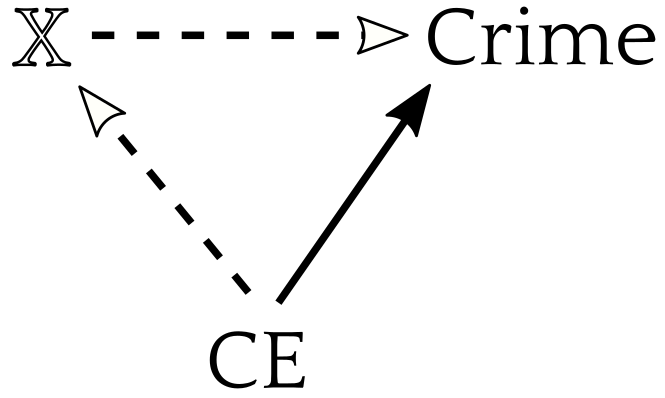
\includegraphics[width=0.4\linewidth]{./figure/appendix/1_omitted_mediator} 

}

\caption{An omitted mediator}\label{fig:dag1}
\end{figure}
Figure \ref{fig:dag1} depicts a simple model where collective efficacy predicts crime directly and through one or more unobserved mediators (\(X\)). For simplicity, assume adjustment for relevant variables which precede collective efficacy and influence crime. In Figure \ref{fig:dag1}, the omitted variable is only a mediator between collective efficacy and crime. Omitting it has no consequence for estimating the total effect of collective efficacy on crime, but including the omitted variable would increase explained variance and tell us more about how collective efficacy influences crime---the omitted variable can be considered a causal mechanism. For the full mediated causal path to be identified, assignment of the treatment (\(CE\)) and the mediator (\(X\)) must satisfy sequential ignorability. There are many candidates for omitted (but inconsequential) mediators, but the present work focuses on criminal opportunities, particularly criminogenic features of the built environment.
\begin{figure}

{\centering 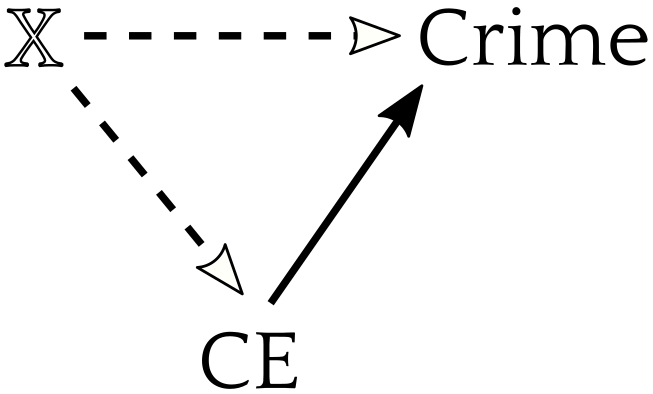
\includegraphics[width=0.4\linewidth]{./figure/appendix/2_spuriousness} 

}

\caption{Spuriousness}\label{fig:dag2}
\end{figure}
Figure \ref{fig:dag2} includes the same variables but inverts the direction of causality between collective efficacy and the omitted measure. \(X\) is now a preceding omitted variable which renders the relationship between collective efficacy and crime partly spurious. This variable must be adjusted for to identify the causal effect of interest. The present work suggests criminogenic features of the built environment as a candidate for these immediate effects on crime and collective efficacy. Because the built environment changes slowly, it is not a plausible mediator for present collective efficacy, though it may moderate its effects. Social factors like legal cynicism or satisfaction with police (Kirk and Matsuda 2011; Sampson and Bartusch 1998) may also occupy this role, though they could just as plausibly be mediators for collective efficacy or simply share the same antecedents. Adjudicating between different causal directions requires repeated observations or instrumental variables.
\begin{figure}

{\centering 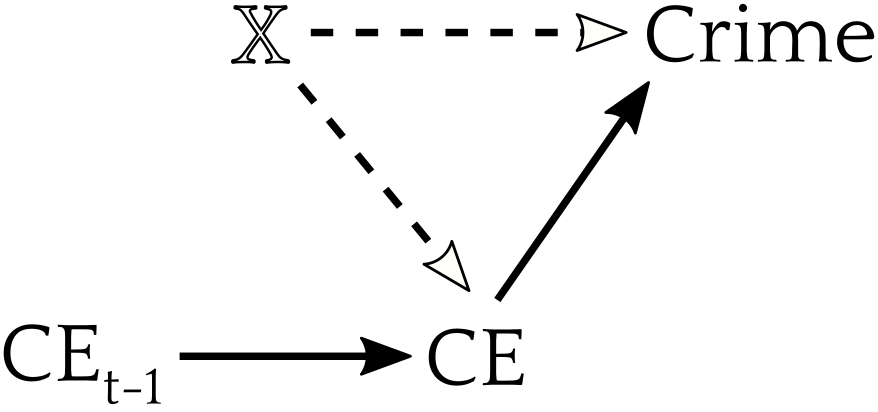
\includegraphics[width=0.5\linewidth]{./figure/appendix/3_instrument} 

}

\caption{A valid instrument}\label{fig:dag3}
\end{figure}
If ignorability cannot be achieved by directly conditioning on all relevant variables---that is some source of spuriousness is unobserved---identification can be achieved using an instrumental variable. Figure \ref{fig:dag3} uses past collective efficacy as an example under the assumption that the only pathway by which past collective efficacy impacts crime is via present collective efficacy or included controls (again, hidden for simplicity). This is a strong and generally untestable assumption. Instrumental variables also assume a monotonic relationship between instrument and treatment. The estimated causal effect provided an instrument is restricted to the subsample for which the instrument induced a change in the treatment---the local average treatment effect (LATE), sometimes called the complier average causal effect.

As an example of instrumental variables, Sampson and Raudenbush (1999) used a series of models with (1) reciprocated exchange and resident attachment to the neighborhood as instruments for collective efficacy, (2) mixed land use as an instrument for disorder, and (3) prior homicide as an instrument for present homicide and robbery. Using these instruments makes the strong assumptions that (1) reciprocated exchange and attachment do not influence crime or disorder through any pathways other than via collective efficacy, (2) mixed land use does not influence crime or collective efficacy except via disorder, and (3) prior homicide does not influence disorder or crime except via present homicide. The present work and recent research by others suggest mixed land use directly influences crime (Wo 2019) and prior crime depresses collective efficacy (Sampson 2012). Due to the interdependence of neighborhood processes, instrumental variables are not a promising route to causal identification unless they are produced via interventions.
\begin{figure}

{\centering 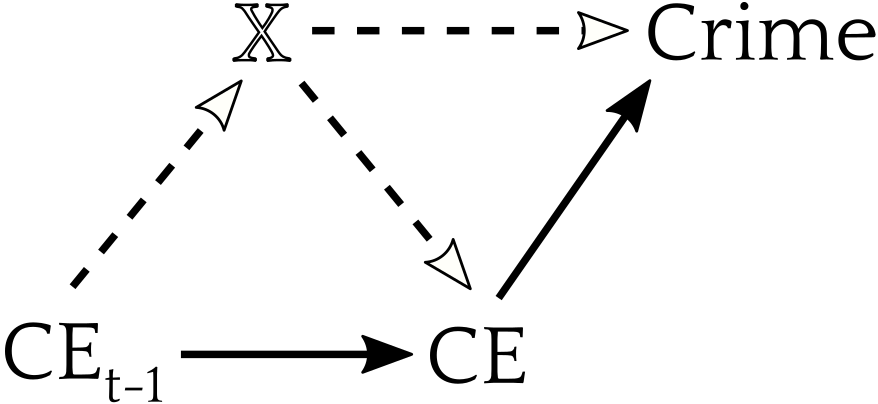
\includegraphics[width=0.5\linewidth]{./figure/appendix/4_bad_instrument} 

}

\caption{Exclusion restriction violation}\label{fig:dag4}
\end{figure}
Figure \ref{fig:dag4} depicts a violation of the exclusion assumption in which past collective efficacy causes one or more of the relevant omitted variables. In this case, use of the instrument will not identify the effect of present collective efficacy on crime because of the backdoor path via \(X\). The present work suggests some characteristics of the built environment occupy the role of \(X\) here by presenting opportunities which facilitate crime while impacting present collective efficacy---but these opportunities may be removed due to collective action of residents, making them dependent on past collective efficacy. While the direct effect of collective efficacy on crime is not identified here, the total effect of past collective efficacy is because the omitted path is entirely descended from past collective efficacy.
\begin{figure}

{\centering \includegraphics[width=0.5\linewidth]{./figure/appendix/4-5_be_model} 

}

\caption{Mediation model}\label{fig:dag45}
\end{figure}
If we observe and include the previously omitted mediator, we arrive at Figure \ref{fig:dag45}. In this model, the effect of present collective efficacy on crime is identified as is the mediation of past collective efficacy through the built environment. Note here the built environment serves as a post-treatment confounder for present collective efficacy which violates sequential ignorability (Imai et al. 2011). Adjusting for the built environment is required to identify the path from present collective efficacy to crime but doing so introduces bias into the estimated intertemporal collective efficacy path. The mediated effect of past collective efficacy on crime via present collective efficacy is thus unidentified. Even in a system with no unobserved variables, some causal effects may not be estimable without making additional assumptions, such as treatment homogeneity (Imai et al. 2011).
\begin{figure}

{\centering \includegraphics[width=0.6\linewidth]{./figure/appendix/5_blocked_path} 

}

\caption{A seemingly valid specification}\label{fig:dag5}
\end{figure}
Including the relevant omitted variables---here the built environment---can close the problematic pathways and render our effect of interest identifiable. Figure \ref{fig:dag5} depicts a DAG in which the built environment is observed. Because the present built environment impacts present collective efficacy, it is logical to include the past built environment in this diagram, though it may be unobservable. Here the past built environment influences both past and present collective efficacy. In this example, the effects of the present built environment and collective efficacy on crime are identified even though none of the other pathways are. In this situation, the total effect of past collective efficacy on present crime cannot be estimated; the first stage of our sequential ignorability has been violated. The mediation pathway from the built environment to crime via collective efficacy would be identified here if all impact of the past built environment on present collective efficacy was mediated by past collective efficacy and the present built environment.
\begin{figure}

{\centering \includegraphics[width=0.6\linewidth]{./figure/appendix/6_still_blocked} 

}

\caption{A non-problematic omitted variable}\label{fig:dag6}
\end{figure}
We might then consider the consequences of additional omitted variables with varying relationships with the observed variables and unobserved past built environment. In Figure \ref{fig:dag6}, I include an unobserved variable \(X\) which is descended from the past built environment and collective efficacy and influences present collective efficacy. Candidates for \(X\) include elements of the built environment for which we do not have measures but increase (or decrease) collective efficacy, such as public spaces which increase interaction between residents and foster collective efficacy. Another obvious candidate for \(X\) here is crime in the past period, which depends on both collective efficacy and the built environment and is known to impact future collective efficacy (Sampson 2012). Investment in the neighborhood from outside sources may also occupy a similar role but operating through the present built environment. So long as these omitted variables operate only through observable antecedents of present crime---collective efficacy or the built environment---they do not compromise our ability to identify the direct causal effects on crime. The causal mediation paths from past collective efficacy through either built the environment or present collective efficacy are not identified here however.
\begin{figure}

{\centering \includegraphics[width=0.6\linewidth]{./figure/appendix/7_backdoor_path} 

}

\caption{A problematic omitted variable}\label{fig:dag7}
\end{figure}
An omitted variable \(X\) which causes crime, as seen in Figure \ref{fig:dag7}, becomes more problematic. If it also causes present collective efficacy or the built environment, or---as shown---is caused by any unobserved antecedent of the built environment or present (but not past) collective efficacy, it will induce bias in our causal estimates of interest. This is likely to be the case for unobserved features of the built environment which provide criminal opportunities. This will also occur if past crime exerts a direct effect on present crime that is not mediated by collective efficacy or the built environment. Fortunately, it is possible to test model sensitivity to unobserved confounders of this sort using methods proposed by Imai, Keele, and Yamamoto (2010). This sensitivity test procedure is similar in principle to that of Harding (2003) in that it simulates varying levels of confounding to determine how strong an omitted confounder would need to be to alter substantive findings.

\hypertarget{bemoderation}{%
\chapter{Built Environment Moderation}\label{bemoderation}}

Early intervention in the built environment may have the added benefit of reducing future social control burdens. The absence of criminogenic features may explain low crime in areas lacking collective efficacy. Conversely, the presence of criminogenic features may make crime ``sticky'' even in the presence of concerted action by residents (St. Jean 2007). This means collective efficacy could be more effective at restraining crime in the absence of environmental features that inhibit the exercise of informal control. Consequently, I expect characteristics of the built environment to moderate the effect of collective efficacy on crime.

This alternate set of models tests whether features of the built environment moderate the association between collective efficacy and crime. These models mirror the prior models of crime but introduce interaction terms between collective efficacy and the built environment features. Based on my theoretical framework, I expect all interactions between collective efficacy and built environment characteristics to be positive because criminogenic features of the environment will attenuate the negative the effect of informal social control on crime.

\hypertarget{crime-and-moderation-of-collective-efficacy-results}{%
\section{Crime and Moderation of Collective Efficacy Results}\label{crime-and-moderation-of-collective-efficacy-results}}

The last set of models augments the original set examining associations with crime with interaction terms between collective efficacy and each of the hypothesized criminogenic built environment features. Interaction terms permit evaluating whether these features present challenges---``ecological disadvantage'' in St. Jean (2007) terms---which are resistant to social control efforts; that is, locations where the returns to collective efficacy are low. Given the weak associations between collective efficacy and each form of crime, and the modest sample size which results in underpowered tests of interaction, these results should be interpreted with caution. Only very strong relationships are likely to be detected, but they may also be the result of sampling error and excessive partitioning of limited variation.

\providecommand{\docline}[3]{\noalign{\global\setlength{\arrayrulewidth}{#1}}\arrayrulecolor[HTML]{#2}\cline{#3}}

\setlength{\tabcolsep}{4pt}

\renewcommand*{\arraystretch}{0.65}
\begin{longtable}[c]{|p{0.10in}|p{0.80in}|p{0.75in}|p{0.75in}|p{0.75in}|p{0.75in}|p{0.75in}}

\caption{\label{tab:secondstageint} Negative Binomial Estimates of Crime}\label{tab:unnamed-chunk-7}\\

\hhline{>{\arrayrulecolor[HTML]{000000}\global\arrayrulewidth=1pt}->{\arrayrulecolor[HTML]{000000}\global\arrayrulewidth=1pt}->{\arrayrulecolor[HTML]{000000}\global\arrayrulewidth=1pt}->{\arrayrulecolor[HTML]{000000}\global\arrayrulewidth=1pt}->{\arrayrulecolor[HTML]{000000}\global\arrayrulewidth=1pt}->{\arrayrulecolor[HTML]{000000}\global\arrayrulewidth=1pt}->{\arrayrulecolor[HTML]{000000}\global\arrayrulewidth=1pt}-}

\multicolumn{1}{!{\color[HTML]{000000}\vrule width 0pt}>{\raggedright}p{\dimexpr 0.1in+0\tabcolsep+0\arrayrulewidth}}{\fontsize{10}{10}\selectfont{\textcolor[HTML]{000000}{\global\setmainfont{Latin Modern Roman}Level}}} & \multicolumn{1}{!{\color[HTML]{000000}\vrule width 0pt}>{\raggedright}p{\dimexpr 0.8in+0\tabcolsep+0\arrayrulewidth}}{\fontsize{10}{10}\selectfont{\textcolor[HTML]{000000}{\global\setmainfont{Latin Modern Roman}}}} & \multicolumn{1}{!{\color[HTML]{000000}\vrule width 0pt}>{\centering}p{\dimexpr 0.75in+0\tabcolsep+0\arrayrulewidth}}{\fontsize{10}{10}\selectfont{\textcolor[HTML]{000000}{\global\setmainfont{Latin Modern Roman}Homicide}}} & \multicolumn{1}{!{\color[HTML]{000000}\vrule width 0pt}>{\centering}p{\dimexpr 0.75in+0\tabcolsep+0\arrayrulewidth}}{\fontsize{10}{10}\selectfont{\textcolor[HTML]{000000}{\global\setmainfont{Latin Modern Roman}Gun Assault}}} & \multicolumn{1}{!{\color[HTML]{000000}\vrule width 0pt}>{\centering}p{\dimexpr 0.75in+0\tabcolsep+0\arrayrulewidth}}{\fontsize{10}{10}\selectfont{\textcolor[HTML]{000000}{\global\setmainfont{Latin Modern Roman}Robbery}}} & \multicolumn{1}{!{\color[HTML]{000000}\vrule width 0pt}>{\centering}p{\dimexpr 0.75in+0\tabcolsep+0\arrayrulewidth}}{\fontsize{10}{10}\selectfont{\textcolor[HTML]{000000}{\global\setmainfont{Latin Modern Roman}Violent}}} & \multicolumn{1}{!{\color[HTML]{000000}\vrule width 0pt}>{\centering}p{\dimexpr 0.75in+0\tabcolsep+0\arrayrulewidth}!{\color[HTML]{000000}\vrule width 0pt}}{\fontsize{10}{10}\selectfont{\textcolor[HTML]{000000}{\global\setmainfont{Latin Modern Roman}Property}}} \\

\noalign{\global\setlength{\arrayrulewidth}{0.5pt}}\arrayrulecolor[HTML]{000000}\cline{1-7}

\endfirsthead

\hhline{>{\arrayrulecolor[HTML]{000000}\global\arrayrulewidth=1pt}->{\arrayrulecolor[HTML]{000000}\global\arrayrulewidth=1pt}->{\arrayrulecolor[HTML]{000000}\global\arrayrulewidth=1pt}->{\arrayrulecolor[HTML]{000000}\global\arrayrulewidth=1pt}->{\arrayrulecolor[HTML]{000000}\global\arrayrulewidth=1pt}->{\arrayrulecolor[HTML]{000000}\global\arrayrulewidth=1pt}->{\arrayrulecolor[HTML]{000000}\global\arrayrulewidth=1pt}-}

\multicolumn{1}{!{\color[HTML]{000000}\vrule width 0pt}>{\raggedright}p{\dimexpr 0.1in+0\tabcolsep+0\arrayrulewidth}}{\fontsize{10}{10}\selectfont{\textcolor[HTML]{000000}{\global\setmainfont{Latin Modern Roman}Level}}} & \multicolumn{1}{!{\color[HTML]{000000}\vrule width 0pt}>{\raggedright}p{\dimexpr 0.8in+0\tabcolsep+0\arrayrulewidth}}{\fontsize{10}{10}\selectfont{\textcolor[HTML]{000000}{\global\setmainfont{Latin Modern Roman}}}} & \multicolumn{1}{!{\color[HTML]{000000}\vrule width 0pt}>{\centering}p{\dimexpr 0.75in+0\tabcolsep+0\arrayrulewidth}}{\fontsize{10}{10}\selectfont{\textcolor[HTML]{000000}{\global\setmainfont{Latin Modern Roman}Homicide}}} & \multicolumn{1}{!{\color[HTML]{000000}\vrule width 0pt}>{\centering}p{\dimexpr 0.75in+0\tabcolsep+0\arrayrulewidth}}{\fontsize{10}{10}\selectfont{\textcolor[HTML]{000000}{\global\setmainfont{Latin Modern Roman}Gun Assault}}} & \multicolumn{1}{!{\color[HTML]{000000}\vrule width 0pt}>{\centering}p{\dimexpr 0.75in+0\tabcolsep+0\arrayrulewidth}}{\fontsize{10}{10}\selectfont{\textcolor[HTML]{000000}{\global\setmainfont{Latin Modern Roman}Robbery}}} & \multicolumn{1}{!{\color[HTML]{000000}\vrule width 0pt}>{\centering}p{\dimexpr 0.75in+0\tabcolsep+0\arrayrulewidth}}{\fontsize{10}{10}\selectfont{\textcolor[HTML]{000000}{\global\setmainfont{Latin Modern Roman}Violent}}} & \multicolumn{1}{!{\color[HTML]{000000}\vrule width 0pt}>{\centering}p{\dimexpr 0.75in+0\tabcolsep+0\arrayrulewidth}!{\color[HTML]{000000}\vrule width 0pt}}{\fontsize{10}{10}\selectfont{\textcolor[HTML]{000000}{\global\setmainfont{Latin Modern Roman}Property}}} \\

\noalign{\global\setlength{\arrayrulewidth}{0.5pt}}\arrayrulecolor[HTML]{000000}\cline{1-7}\endhead



\multicolumn{7}{!{\color[HTML]{000000}\vrule width 0pt}>{\raggedright}p{\dimexpr 4.65in+12\tabcolsep+6\arrayrulewidth}}{\fontsize{10}{10}\selectfont{\textcolor[HTML]{000000}{\global\setmainfont{Latin Modern Roman}Neighborhood}}} \\





\multicolumn{1}{!{\color[HTML]{000000}\vrule width 0pt}>{\raggedright}p{\dimexpr 0.1in+0\tabcolsep+0\arrayrulewidth}}{\fontsize{10}{10}\selectfont{\textcolor[HTML]{000000}{\global\setmainfont{Latin Modern Roman}}}} & \multicolumn{1}{!{\color[HTML]{000000}\vrule width 0pt}>{\raggedright}p{\dimexpr 0.8in+0\tabcolsep+0\arrayrulewidth}}{\fontsize{10}{10}\selectfont{\textcolor[HTML]{000000}{\global\setmainfont{Latin Modern Roman}Coll. Eff (2001)}}} & \multicolumn{1}{!{\color[HTML]{000000}\vrule width 0pt}>{\centering}p{\dimexpr 0.75in+0\tabcolsep+0\arrayrulewidth}}{\fontsize{10}{10}\selectfont{\textcolor[HTML]{000000}{\global\setmainfont{Latin Modern Roman}-0.09}}\fontsize{10}{10}\selectfont{\textcolor[HTML]{000000}{\global\setmainfont{Latin Modern Roman}\linebreak }}\fontsize{10}{10}\selectfont{\textcolor[HTML]{000000}{\global\setmainfont{Latin Modern Roman}(}}\fontsize{10}{10}\selectfont{\textcolor[HTML]{000000}{\global\setmainfont{Latin Modern Roman}0.11}}\fontsize{10}{10}\selectfont{\textcolor[HTML]{000000}{\global\setmainfont{Latin Modern Roman})}}} & \multicolumn{1}{!{\color[HTML]{000000}\vrule width 0pt}>{\centering}p{\dimexpr 0.75in+0\tabcolsep+0\arrayrulewidth}}{\fontsize{10}{10}\selectfont{\textcolor[HTML]{000000}{\global\setmainfont{Latin Modern Roman}-0.03}}\fontsize{10}{10}\selectfont{\textcolor[HTML]{000000}{\global\setmainfont{Latin Modern Roman}\linebreak }}\fontsize{10}{10}\selectfont{\textcolor[HTML]{000000}{\global\setmainfont{Latin Modern Roman}(}}\fontsize{10}{10}\selectfont{\textcolor[HTML]{000000}{\global\setmainfont{Latin Modern Roman}0.05}}\fontsize{10}{10}\selectfont{\textcolor[HTML]{000000}{\global\setmainfont{Latin Modern Roman})}}} & \multicolumn{1}{!{\color[HTML]{000000}\vrule width 0pt}>{\centering}p{\dimexpr 0.75in+0\tabcolsep+0\arrayrulewidth}}{\fontsize{10}{10}\selectfont{\textcolor[HTML]{000000}{\global\setmainfont{Latin Modern Roman}-0.07}}\fontsize{10}{10}\selectfont{\textcolor[HTML]{000000}{\global\setmainfont{Latin Modern Roman}\linebreak }}\fontsize{10}{10}\selectfont{\textcolor[HTML]{000000}{\global\setmainfont{Latin Modern Roman}(}}\fontsize{10}{10}\selectfont{\textcolor[HTML]{000000}{\global\setmainfont{Latin Modern Roman}0.04}}\fontsize{10}{10}\selectfont{\textcolor[HTML]{000000}{\global\setmainfont{Latin Modern Roman})}}} & \multicolumn{1}{!{\color[HTML]{000000}\vrule width 0pt}>{\centering}p{\dimexpr 0.75in+0\tabcolsep+0\arrayrulewidth}}{\fontsize{10}{10}\selectfont{\textcolor[HTML]{000000}{\global\setmainfont{Latin Modern Roman}\textbf{-0.09}}}\fontsize{10}{10}\selectfont{\textcolor[HTML]{000000}{\global\setmainfont{Latin Modern Roman}\textbf{\linebreak }}}\fontsize{10}{10}\selectfont{\textcolor[HTML]{000000}{\global\setmainfont{Latin Modern Roman}\textbf{(}}}\fontsize{10}{10}\selectfont{\textcolor[HTML]{000000}{\global\setmainfont{Latin Modern Roman}\textbf{0.04}}}\fontsize{10}{10}\selectfont{\textcolor[HTML]{000000}{\global\setmainfont{Latin Modern Roman}\textbf{)}}}} & \multicolumn{1}{!{\color[HTML]{000000}\vrule width 0pt}>{\centering}p{\dimexpr 0.75in+0\tabcolsep+0\arrayrulewidth}!{\color[HTML]{000000}\vrule width 0pt}}{\fontsize{10}{10}\selectfont{\textcolor[HTML]{000000}{\global\setmainfont{Latin Modern Roman}\textbf{-0.06}}}\fontsize{10}{10}\selectfont{\textcolor[HTML]{000000}{\global\setmainfont{Latin Modern Roman}\textbf{\linebreak }}}\fontsize{10}{10}\selectfont{\textcolor[HTML]{000000}{\global\setmainfont{Latin Modern Roman}\textbf{(}}}\fontsize{10}{10}\selectfont{\textcolor[HTML]{000000}{\global\setmainfont{Latin Modern Roman}\textbf{0.03}}}\fontsize{10}{10}\selectfont{\textcolor[HTML]{000000}{\global\setmainfont{Latin Modern Roman}\textbf{)}}}} \\





\multicolumn{1}{!{\color[HTML]{000000}\vrule width 0pt}>{\raggedright}p{\dimexpr 0.1in+0\tabcolsep+0\arrayrulewidth}}{\fontsize{10}{10}\selectfont{\textcolor[HTML]{000000}{\global\setmainfont{Latin Modern Roman}}}} & \multicolumn{1}{!{\color[HTML]{000000}\vrule width 0pt}>{\raggedright}p{\dimexpr 0.8in+0\tabcolsep+0\arrayrulewidth}}{\fontsize{10}{10}\selectfont{\textcolor[HTML]{000000}{\global\setmainfont{Latin Modern Roman}Disadv.}}} & \multicolumn{1}{!{\color[HTML]{000000}\vrule width 0pt}>{\centering}p{\dimexpr 0.75in+0\tabcolsep+0\arrayrulewidth}}{\fontsize{10}{10}\selectfont{\textcolor[HTML]{000000}{\global\setmainfont{Latin Modern Roman}\textbf{0.54}}}\fontsize{10}{10}\selectfont{\textcolor[HTML]{000000}{\global\setmainfont{Latin Modern Roman}\textbf{\linebreak }}}\fontsize{10}{10}\selectfont{\textcolor[HTML]{000000}{\global\setmainfont{Latin Modern Roman}\textbf{(}}}\fontsize{10}{10}\selectfont{\textcolor[HTML]{000000}{\global\setmainfont{Latin Modern Roman}\textbf{0.11}}}\fontsize{10}{10}\selectfont{\textcolor[HTML]{000000}{\global\setmainfont{Latin Modern Roman}\textbf{)}}}} & \multicolumn{1}{!{\color[HTML]{000000}\vrule width 0pt}>{\centering}p{\dimexpr 0.75in+0\tabcolsep+0\arrayrulewidth}}{\fontsize{10}{10}\selectfont{\textcolor[HTML]{000000}{\global\setmainfont{Latin Modern Roman}\textbf{0.69}}}\fontsize{10}{10}\selectfont{\textcolor[HTML]{000000}{\global\setmainfont{Latin Modern Roman}\textbf{\linebreak }}}\fontsize{10}{10}\selectfont{\textcolor[HTML]{000000}{\global\setmainfont{Latin Modern Roman}\textbf{(}}}\fontsize{10}{10}\selectfont{\textcolor[HTML]{000000}{\global\setmainfont{Latin Modern Roman}\textbf{0.05}}}\fontsize{10}{10}\selectfont{\textcolor[HTML]{000000}{\global\setmainfont{Latin Modern Roman}\textbf{)}}}} & \multicolumn{1}{!{\color[HTML]{000000}\vrule width 0pt}>{\centering}p{\dimexpr 0.75in+0\tabcolsep+0\arrayrulewidth}}{\fontsize{10}{10}\selectfont{\textcolor[HTML]{000000}{\global\setmainfont{Latin Modern Roman}\textbf{0.22}}}\fontsize{10}{10}\selectfont{\textcolor[HTML]{000000}{\global\setmainfont{Latin Modern Roman}\textbf{\linebreak }}}\fontsize{10}{10}\selectfont{\textcolor[HTML]{000000}{\global\setmainfont{Latin Modern Roman}\textbf{(}}}\fontsize{10}{10}\selectfont{\textcolor[HTML]{000000}{\global\setmainfont{Latin Modern Roman}\textbf{0.04}}}\fontsize{10}{10}\selectfont{\textcolor[HTML]{000000}{\global\setmainfont{Latin Modern Roman}\textbf{)}}}} & \multicolumn{1}{!{\color[HTML]{000000}\vrule width 0pt}>{\centering}p{\dimexpr 0.75in+0\tabcolsep+0\arrayrulewidth}}{\fontsize{10}{10}\selectfont{\textcolor[HTML]{000000}{\global\setmainfont{Latin Modern Roman}\textbf{0.38}}}\fontsize{10}{10}\selectfont{\textcolor[HTML]{000000}{\global\setmainfont{Latin Modern Roman}\textbf{\linebreak }}}\fontsize{10}{10}\selectfont{\textcolor[HTML]{000000}{\global\setmainfont{Latin Modern Roman}\textbf{(}}}\fontsize{10}{10}\selectfont{\textcolor[HTML]{000000}{\global\setmainfont{Latin Modern Roman}\textbf{0.04}}}\fontsize{10}{10}\selectfont{\textcolor[HTML]{000000}{\global\setmainfont{Latin Modern Roman}\textbf{)}}}} & \multicolumn{1}{!{\color[HTML]{000000}\vrule width 0pt}>{\centering}p{\dimexpr 0.75in+0\tabcolsep+0\arrayrulewidth}!{\color[HTML]{000000}\vrule width 0pt}}{\fontsize{10}{10}\selectfont{\textcolor[HTML]{000000}{\global\setmainfont{Latin Modern Roman}\textbf{-0.09}}}\fontsize{10}{10}\selectfont{\textcolor[HTML]{000000}{\global\setmainfont{Latin Modern Roman}\textbf{\linebreak }}}\fontsize{10}{10}\selectfont{\textcolor[HTML]{000000}{\global\setmainfont{Latin Modern Roman}\textbf{(}}}\fontsize{10}{10}\selectfont{\textcolor[HTML]{000000}{\global\setmainfont{Latin Modern Roman}\textbf{0.03}}}\fontsize{10}{10}\selectfont{\textcolor[HTML]{000000}{\global\setmainfont{Latin Modern Roman}\textbf{)}}}} \\





\multicolumn{1}{!{\color[HTML]{000000}\vrule width 0pt}>{\raggedright}p{\dimexpr 0.1in+0\tabcolsep+0\arrayrulewidth}}{\fontsize{10}{10}\selectfont{\textcolor[HTML]{000000}{\global\setmainfont{Latin Modern Roman}}}} & \multicolumn{1}{!{\color[HTML]{000000}\vrule width 0pt}>{\raggedright}p{\dimexpr 0.8in+0\tabcolsep+0\arrayrulewidth}}{\fontsize{10}{10}\selectfont{\textcolor[HTML]{000000}{\global\setmainfont{Latin Modern Roman}Stability}}} & \multicolumn{1}{!{\color[HTML]{000000}\vrule width 0pt}>{\centering}p{\dimexpr 0.75in+0\tabcolsep+0\arrayrulewidth}}{\fontsize{10}{10}\selectfont{\textcolor[HTML]{000000}{\global\setmainfont{Latin Modern Roman}-0.03}}\fontsize{10}{10}\selectfont{\textcolor[HTML]{000000}{\global\setmainfont{Latin Modern Roman}\linebreak }}\fontsize{10}{10}\selectfont{\textcolor[HTML]{000000}{\global\setmainfont{Latin Modern Roman}(}}\fontsize{10}{10}\selectfont{\textcolor[HTML]{000000}{\global\setmainfont{Latin Modern Roman}0.13}}\fontsize{10}{10}\selectfont{\textcolor[HTML]{000000}{\global\setmainfont{Latin Modern Roman})}}} & \multicolumn{1}{!{\color[HTML]{000000}\vrule width 0pt}>{\centering}p{\dimexpr 0.75in+0\tabcolsep+0\arrayrulewidth}}{\fontsize{10}{10}\selectfont{\textcolor[HTML]{000000}{\global\setmainfont{Latin Modern Roman}-0.02}}\fontsize{10}{10}\selectfont{\textcolor[HTML]{000000}{\global\setmainfont{Latin Modern Roman}\linebreak }}\fontsize{10}{10}\selectfont{\textcolor[HTML]{000000}{\global\setmainfont{Latin Modern Roman}(}}\fontsize{10}{10}\selectfont{\textcolor[HTML]{000000}{\global\setmainfont{Latin Modern Roman}0.06}}\fontsize{10}{10}\selectfont{\textcolor[HTML]{000000}{\global\setmainfont{Latin Modern Roman})}}} & \multicolumn{1}{!{\color[HTML]{000000}\vrule width 0pt}>{\centering}p{\dimexpr 0.75in+0\tabcolsep+0\arrayrulewidth}}{\fontsize{10}{10}\selectfont{\textcolor[HTML]{000000}{\global\setmainfont{Latin Modern Roman}\textbf{0.16}}}\fontsize{10}{10}\selectfont{\textcolor[HTML]{000000}{\global\setmainfont{Latin Modern Roman}\textbf{\linebreak }}}\fontsize{10}{10}\selectfont{\textcolor[HTML]{000000}{\global\setmainfont{Latin Modern Roman}\textbf{(}}}\fontsize{10}{10}\selectfont{\textcolor[HTML]{000000}{\global\setmainfont{Latin Modern Roman}\textbf{0.05}}}\fontsize{10}{10}\selectfont{\textcolor[HTML]{000000}{\global\setmainfont{Latin Modern Roman}\textbf{)}}}} & \multicolumn{1}{!{\color[HTML]{000000}\vrule width 0pt}>{\centering}p{\dimexpr 0.75in+0\tabcolsep+0\arrayrulewidth}}{\fontsize{10}{10}\selectfont{\textcolor[HTML]{000000}{\global\setmainfont{Latin Modern Roman}\textbf{0.14}}}\fontsize{10}{10}\selectfont{\textcolor[HTML]{000000}{\global\setmainfont{Latin Modern Roman}\textbf{\linebreak }}}\fontsize{10}{10}\selectfont{\textcolor[HTML]{000000}{\global\setmainfont{Latin Modern Roman}\textbf{(}}}\fontsize{10}{10}\selectfont{\textcolor[HTML]{000000}{\global\setmainfont{Latin Modern Roman}\textbf{0.04}}}\fontsize{10}{10}\selectfont{\textcolor[HTML]{000000}{\global\setmainfont{Latin Modern Roman}\textbf{)}}}} & \multicolumn{1}{!{\color[HTML]{000000}\vrule width 0pt}>{\centering}p{\dimexpr 0.75in+0\tabcolsep+0\arrayrulewidth}!{\color[HTML]{000000}\vrule width 0pt}}{\fontsize{10}{10}\selectfont{\textcolor[HTML]{000000}{\global\setmainfont{Latin Modern Roman}\textbf{0.29}}}\fontsize{10}{10}\selectfont{\textcolor[HTML]{000000}{\global\setmainfont{Latin Modern Roman}\textbf{\linebreak }}}\fontsize{10}{10}\selectfont{\textcolor[HTML]{000000}{\global\setmainfont{Latin Modern Roman}\textbf{(}}}\fontsize{10}{10}\selectfont{\textcolor[HTML]{000000}{\global\setmainfont{Latin Modern Roman}\textbf{0.03}}}\fontsize{10}{10}\selectfont{\textcolor[HTML]{000000}{\global\setmainfont{Latin Modern Roman}\textbf{)}}}} \\





\multicolumn{1}{!{\color[HTML]{000000}\vrule width 0pt}>{\raggedright}p{\dimexpr 0.1in+0\tabcolsep+0\arrayrulewidth}}{\fontsize{10}{10}\selectfont{\textcolor[HTML]{000000}{\global\setmainfont{Latin Modern Roman}}}} & \multicolumn{1}{!{\color[HTML]{000000}\vrule width 0pt}>{\raggedright}p{\dimexpr 0.8in+0\tabcolsep+0\arrayrulewidth}}{\fontsize{10}{10}\selectfont{\textcolor[HTML]{000000}{\global\setmainfont{Latin Modern Roman}Hispanic /\linebreak Immigrant}}} & \multicolumn{1}{!{\color[HTML]{000000}\vrule width 0pt}>{\centering}p{\dimexpr 0.75in+0\tabcolsep+0\arrayrulewidth}}{\fontsize{10}{10}\selectfont{\textcolor[HTML]{000000}{\global\setmainfont{Latin Modern Roman}\textbf{-0.35}}}\fontsize{10}{10}\selectfont{\textcolor[HTML]{000000}{\global\setmainfont{Latin Modern Roman}\textbf{\linebreak }}}\fontsize{10}{10}\selectfont{\textcolor[HTML]{000000}{\global\setmainfont{Latin Modern Roman}\textbf{(}}}\fontsize{10}{10}\selectfont{\textcolor[HTML]{000000}{\global\setmainfont{Latin Modern Roman}\textbf{0.11}}}\fontsize{10}{10}\selectfont{\textcolor[HTML]{000000}{\global\setmainfont{Latin Modern Roman}\textbf{)}}}} & \multicolumn{1}{!{\color[HTML]{000000}\vrule width 0pt}>{\centering}p{\dimexpr 0.75in+0\tabcolsep+0\arrayrulewidth}}{\fontsize{10}{10}\selectfont{\textcolor[HTML]{000000}{\global\setmainfont{Latin Modern Roman}\textbf{-0.16}}}\fontsize{10}{10}\selectfont{\textcolor[HTML]{000000}{\global\setmainfont{Latin Modern Roman}\textbf{\linebreak }}}\fontsize{10}{10}\selectfont{\textcolor[HTML]{000000}{\global\setmainfont{Latin Modern Roman}\textbf{(}}}\fontsize{10}{10}\selectfont{\textcolor[HTML]{000000}{\global\setmainfont{Latin Modern Roman}\textbf{0.05}}}\fontsize{10}{10}\selectfont{\textcolor[HTML]{000000}{\global\setmainfont{Latin Modern Roman}\textbf{)}}}} & \multicolumn{1}{!{\color[HTML]{000000}\vrule width 0pt}>{\centering}p{\dimexpr 0.75in+0\tabcolsep+0\arrayrulewidth}}{\fontsize{10}{10}\selectfont{\textcolor[HTML]{000000}{\global\setmainfont{Latin Modern Roman}\textbf{-0.41}}}\fontsize{10}{10}\selectfont{\textcolor[HTML]{000000}{\global\setmainfont{Latin Modern Roman}\textbf{\linebreak }}}\fontsize{10}{10}\selectfont{\textcolor[HTML]{000000}{\global\setmainfont{Latin Modern Roman}\textbf{(}}}\fontsize{10}{10}\selectfont{\textcolor[HTML]{000000}{\global\setmainfont{Latin Modern Roman}\textbf{0.04}}}\fontsize{10}{10}\selectfont{\textcolor[HTML]{000000}{\global\setmainfont{Latin Modern Roman}\textbf{)}}}} & \multicolumn{1}{!{\color[HTML]{000000}\vrule width 0pt}>{\centering}p{\dimexpr 0.75in+0\tabcolsep+0\arrayrulewidth}}{\fontsize{10}{10}\selectfont{\textcolor[HTML]{000000}{\global\setmainfont{Latin Modern Roman}\textbf{-0.33}}}\fontsize{10}{10}\selectfont{\textcolor[HTML]{000000}{\global\setmainfont{Latin Modern Roman}\textbf{\linebreak }}}\fontsize{10}{10}\selectfont{\textcolor[HTML]{000000}{\global\setmainfont{Latin Modern Roman}\textbf{(}}}\fontsize{10}{10}\selectfont{\textcolor[HTML]{000000}{\global\setmainfont{Latin Modern Roman}\textbf{0.03}}}\fontsize{10}{10}\selectfont{\textcolor[HTML]{000000}{\global\setmainfont{Latin Modern Roman}\textbf{)}}}} & \multicolumn{1}{!{\color[HTML]{000000}\vrule width 0pt}>{\centering}p{\dimexpr 0.75in+0\tabcolsep+0\arrayrulewidth}!{\color[HTML]{000000}\vrule width 0pt}}{\fontsize{10}{10}\selectfont{\textcolor[HTML]{000000}{\global\setmainfont{Latin Modern Roman}\textbf{-0.23}}}\fontsize{10}{10}\selectfont{\textcolor[HTML]{000000}{\global\setmainfont{Latin Modern Roman}\textbf{\linebreak }}}\fontsize{10}{10}\selectfont{\textcolor[HTML]{000000}{\global\setmainfont{Latin Modern Roman}\textbf{(}}}\fontsize{10}{10}\selectfont{\textcolor[HTML]{000000}{\global\setmainfont{Latin Modern Roman}\textbf{0.03}}}\fontsize{10}{10}\selectfont{\textcolor[HTML]{000000}{\global\setmainfont{Latin Modern Roman}\textbf{)}}}} \\





\multicolumn{1}{!{\color[HTML]{000000}\vrule width 0pt}>{\raggedright}p{\dimexpr 0.1in+0\tabcolsep+0\arrayrulewidth}}{\fontsize{10}{10}\selectfont{\textcolor[HTML]{000000}{\global\setmainfont{Latin Modern Roman}}}} & \multicolumn{1}{!{\color[HTML]{000000}\vrule width 0pt}>{\raggedright}p{\dimexpr 0.8in+0\tabcolsep+0\arrayrulewidth}}{\fontsize{10}{10}\selectfont{\textcolor[HTML]{000000}{\global\setmainfont{Latin Modern Roman}Density (Neighb.)}}} & \multicolumn{1}{!{\color[HTML]{000000}\vrule width 0pt}>{\centering}p{\dimexpr 0.75in+0\tabcolsep+0\arrayrulewidth}}{\fontsize{10}{10}\selectfont{\textcolor[HTML]{000000}{\global\setmainfont{Latin Modern Roman}\textbf{0.24}}}\fontsize{10}{10}\selectfont{\textcolor[HTML]{000000}{\global\setmainfont{Latin Modern Roman}\textbf{\linebreak }}}\fontsize{10}{10}\selectfont{\textcolor[HTML]{000000}{\global\setmainfont{Latin Modern Roman}\textbf{(}}}\fontsize{10}{10}\selectfont{\textcolor[HTML]{000000}{\global\setmainfont{Latin Modern Roman}\textbf{0.11}}}\fontsize{10}{10}\selectfont{\textcolor[HTML]{000000}{\global\setmainfont{Latin Modern Roman}\textbf{)}}}} & \multicolumn{1}{!{\color[HTML]{000000}\vrule width 0pt}>{\centering}p{\dimexpr 0.75in+0\tabcolsep+0\arrayrulewidth}}{\fontsize{10}{10}\selectfont{\textcolor[HTML]{000000}{\global\setmainfont{Latin Modern Roman}0.06}}\fontsize{10}{10}\selectfont{\textcolor[HTML]{000000}{\global\setmainfont{Latin Modern Roman}\linebreak }}\fontsize{10}{10}\selectfont{\textcolor[HTML]{000000}{\global\setmainfont{Latin Modern Roman}(}}\fontsize{10}{10}\selectfont{\textcolor[HTML]{000000}{\global\setmainfont{Latin Modern Roman}0.06}}\fontsize{10}{10}\selectfont{\textcolor[HTML]{000000}{\global\setmainfont{Latin Modern Roman})}}} & \multicolumn{1}{!{\color[HTML]{000000}\vrule width 0pt}>{\centering}p{\dimexpr 0.75in+0\tabcolsep+0\arrayrulewidth}}{\fontsize{10}{10}\selectfont{\textcolor[HTML]{000000}{\global\setmainfont{Latin Modern Roman}\textbf{0.25}}}\fontsize{10}{10}\selectfont{\textcolor[HTML]{000000}{\global\setmainfont{Latin Modern Roman}\textbf{\linebreak }}}\fontsize{10}{10}\selectfont{\textcolor[HTML]{000000}{\global\setmainfont{Latin Modern Roman}\textbf{(}}}\fontsize{10}{10}\selectfont{\textcolor[HTML]{000000}{\global\setmainfont{Latin Modern Roman}\textbf{0.05}}}\fontsize{10}{10}\selectfont{\textcolor[HTML]{000000}{\global\setmainfont{Latin Modern Roman}\textbf{)}}}} & \multicolumn{1}{!{\color[HTML]{000000}\vrule width 0pt}>{\centering}p{\dimexpr 0.75in+0\tabcolsep+0\arrayrulewidth}}{\fontsize{10}{10}\selectfont{\textcolor[HTML]{000000}{\global\setmainfont{Latin Modern Roman}\textbf{0.16}}}\fontsize{10}{10}\selectfont{\textcolor[HTML]{000000}{\global\setmainfont{Latin Modern Roman}\textbf{\linebreak }}}\fontsize{10}{10}\selectfont{\textcolor[HTML]{000000}{\global\setmainfont{Latin Modern Roman}\textbf{(}}}\fontsize{10}{10}\selectfont{\textcolor[HTML]{000000}{\global\setmainfont{Latin Modern Roman}\textbf{0.04}}}\fontsize{10}{10}\selectfont{\textcolor[HTML]{000000}{\global\setmainfont{Latin Modern Roman}\textbf{)}}}} & \multicolumn{1}{!{\color[HTML]{000000}\vrule width 0pt}>{\centering}p{\dimexpr 0.75in+0\tabcolsep+0\arrayrulewidth}!{\color[HTML]{000000}\vrule width 0pt}}{\fontsize{10}{10}\selectfont{\textcolor[HTML]{000000}{\global\setmainfont{Latin Modern Roman}\textbf{0.09}}}\fontsize{10}{10}\selectfont{\textcolor[HTML]{000000}{\global\setmainfont{Latin Modern Roman}\textbf{\linebreak }}}\fontsize{10}{10}\selectfont{\textcolor[HTML]{000000}{\global\setmainfont{Latin Modern Roman}\textbf{(}}}\fontsize{10}{10}\selectfont{\textcolor[HTML]{000000}{\global\setmainfont{Latin Modern Roman}\textbf{0.03}}}\fontsize{10}{10}\selectfont{\textcolor[HTML]{000000}{\global\setmainfont{Latin Modern Roman}\textbf{)}}}} \\





\multicolumn{7}{!{\color[HTML]{000000}\vrule width 0pt}>{\raggedright}p{\dimexpr 4.65in+12\tabcolsep+6\arrayrulewidth}}{\fontsize{10}{10}\selectfont{\textcolor[HTML]{000000}{\global\setmainfont{Latin Modern Roman}Block}}} \\





\multicolumn{1}{!{\color[HTML]{000000}\vrule width 0pt}>{\raggedright}p{\dimexpr 0.1in+0\tabcolsep+0\arrayrulewidth}}{\fontsize{10}{10}\selectfont{\textcolor[HTML]{000000}{\global\setmainfont{Latin Modern Roman}}}} & \multicolumn{1}{!{\color[HTML]{000000}\vrule width 0pt}>{\raggedright}p{\dimexpr 0.8in+0\tabcolsep+0\arrayrulewidth}}{\fontsize{10}{10}\selectfont{\textcolor[HTML]{000000}{\global\setmainfont{Latin Modern Roman}Abandoned}}} & \multicolumn{1}{!{\color[HTML]{000000}\vrule width 0pt}>{\centering}p{\dimexpr 0.75in+0\tabcolsep+0\arrayrulewidth}}{\fontsize{10}{10}\selectfont{\textcolor[HTML]{000000}{\global\setmainfont{Latin Modern Roman}0.17}}\fontsize{10}{10}\selectfont{\textcolor[HTML]{000000}{\global\setmainfont{Latin Modern Roman}\linebreak }}\fontsize{10}{10}\selectfont{\textcolor[HTML]{000000}{\global\setmainfont{Latin Modern Roman}(}}\fontsize{10}{10}\selectfont{\textcolor[HTML]{000000}{\global\setmainfont{Latin Modern Roman}0.09}}\fontsize{10}{10}\selectfont{\textcolor[HTML]{000000}{\global\setmainfont{Latin Modern Roman})}}} & \multicolumn{1}{!{\color[HTML]{000000}\vrule width 0pt}>{\centering}p{\dimexpr 0.75in+0\tabcolsep+0\arrayrulewidth}}{\fontsize{10}{10}\selectfont{\textcolor[HTML]{000000}{\global\setmainfont{Latin Modern Roman}\textbf{0.21}}}\fontsize{10}{10}\selectfont{\textcolor[HTML]{000000}{\global\setmainfont{Latin Modern Roman}\textbf{\linebreak }}}\fontsize{10}{10}\selectfont{\textcolor[HTML]{000000}{\global\setmainfont{Latin Modern Roman}\textbf{(}}}\fontsize{10}{10}\selectfont{\textcolor[HTML]{000000}{\global\setmainfont{Latin Modern Roman}\textbf{0.04}}}\fontsize{10}{10}\selectfont{\textcolor[HTML]{000000}{\global\setmainfont{Latin Modern Roman}\textbf{)}}}} & \multicolumn{1}{!{\color[HTML]{000000}\vrule width 0pt}>{\centering}p{\dimexpr 0.75in+0\tabcolsep+0\arrayrulewidth}}{\fontsize{10}{10}\selectfont{\textcolor[HTML]{000000}{\global\setmainfont{Latin Modern Roman}\textbf{0.10}}}\fontsize{10}{10}\selectfont{\textcolor[HTML]{000000}{\global\setmainfont{Latin Modern Roman}\textbf{\linebreak }}}\fontsize{10}{10}\selectfont{\textcolor[HTML]{000000}{\global\setmainfont{Latin Modern Roman}\textbf{(}}}\fontsize{10}{10}\selectfont{\textcolor[HTML]{000000}{\global\setmainfont{Latin Modern Roman}\textbf{0.03}}}\fontsize{10}{10}\selectfont{\textcolor[HTML]{000000}{\global\setmainfont{Latin Modern Roman}\textbf{)}}}} & \multicolumn{1}{!{\color[HTML]{000000}\vrule width 0pt}>{\centering}p{\dimexpr 0.75in+0\tabcolsep+0\arrayrulewidth}}{\fontsize{10}{10}\selectfont{\textcolor[HTML]{000000}{\global\setmainfont{Latin Modern Roman}\textbf{0.14}}}\fontsize{10}{10}\selectfont{\textcolor[HTML]{000000}{\global\setmainfont{Latin Modern Roman}\textbf{\linebreak }}}\fontsize{10}{10}\selectfont{\textcolor[HTML]{000000}{\global\setmainfont{Latin Modern Roman}\textbf{(}}}\fontsize{10}{10}\selectfont{\textcolor[HTML]{000000}{\global\setmainfont{Latin Modern Roman}\textbf{0.03}}}\fontsize{10}{10}\selectfont{\textcolor[HTML]{000000}{\global\setmainfont{Latin Modern Roman}\textbf{)}}}} & \multicolumn{1}{!{\color[HTML]{000000}\vrule width 0pt}>{\centering}p{\dimexpr 0.75in+0\tabcolsep+0\arrayrulewidth}!{\color[HTML]{000000}\vrule width 0pt}}{\fontsize{10}{10}\selectfont{\textcolor[HTML]{000000}{\global\setmainfont{Latin Modern Roman}\textbf{0.07}}}\fontsize{10}{10}\selectfont{\textcolor[HTML]{000000}{\global\setmainfont{Latin Modern Roman}\textbf{\linebreak }}}\fontsize{10}{10}\selectfont{\textcolor[HTML]{000000}{\global\setmainfont{Latin Modern Roman}\textbf{(}}}\fontsize{10}{10}\selectfont{\textcolor[HTML]{000000}{\global\setmainfont{Latin Modern Roman}\textbf{0.02}}}\fontsize{10}{10}\selectfont{\textcolor[HTML]{000000}{\global\setmainfont{Latin Modern Roman}\textbf{)}}}} \\





\multicolumn{1}{!{\color[HTML]{000000}\vrule width 0pt}>{\raggedright}p{\dimexpr 0.1in+0\tabcolsep+0\arrayrulewidth}}{\fontsize{10}{10}\selectfont{\textcolor[HTML]{000000}{\global\setmainfont{Latin Modern Roman}}}} & \multicolumn{1}{!{\color[HTML]{000000}\vrule width 0pt}>{\raggedright}p{\dimexpr 0.8in+0\tabcolsep+0\arrayrulewidth}}{\fontsize{10}{10}\selectfont{\textcolor[HTML]{000000}{\global\setmainfont{Latin Modern Roman}Bars}}} & \multicolumn{1}{!{\color[HTML]{000000}\vrule width 0pt}>{\centering}p{\dimexpr 0.75in+0\tabcolsep+0\arrayrulewidth}}{\fontsize{10}{10}\selectfont{\textcolor[HTML]{000000}{\global\setmainfont{Latin Modern Roman}0.14}}\fontsize{10}{10}\selectfont{\textcolor[HTML]{000000}{\global\setmainfont{Latin Modern Roman}\linebreak }}\fontsize{10}{10}\selectfont{\textcolor[HTML]{000000}{\global\setmainfont{Latin Modern Roman}(}}\fontsize{10}{10}\selectfont{\textcolor[HTML]{000000}{\global\setmainfont{Latin Modern Roman}0.11}}\fontsize{10}{10}\selectfont{\textcolor[HTML]{000000}{\global\setmainfont{Latin Modern Roman})}}} & \multicolumn{1}{!{\color[HTML]{000000}\vrule width 0pt}>{\centering}p{\dimexpr 0.75in+0\tabcolsep+0\arrayrulewidth}}{\fontsize{10}{10}\selectfont{\textcolor[HTML]{000000}{\global\setmainfont{Latin Modern Roman}0.02}}\fontsize{10}{10}\selectfont{\textcolor[HTML]{000000}{\global\setmainfont{Latin Modern Roman}\linebreak }}\fontsize{10}{10}\selectfont{\textcolor[HTML]{000000}{\global\setmainfont{Latin Modern Roman}(}}\fontsize{10}{10}\selectfont{\textcolor[HTML]{000000}{\global\setmainfont{Latin Modern Roman}0.05}}\fontsize{10}{10}\selectfont{\textcolor[HTML]{000000}{\global\setmainfont{Latin Modern Roman})}}} & \multicolumn{1}{!{\color[HTML]{000000}\vrule width 0pt}>{\centering}p{\dimexpr 0.75in+0\tabcolsep+0\arrayrulewidth}}{\fontsize{10}{10}\selectfont{\textcolor[HTML]{000000}{\global\setmainfont{Latin Modern Roman}-0.05}}\fontsize{10}{10}\selectfont{\textcolor[HTML]{000000}{\global\setmainfont{Latin Modern Roman}\linebreak }}\fontsize{10}{10}\selectfont{\textcolor[HTML]{000000}{\global\setmainfont{Latin Modern Roman}(}}\fontsize{10}{10}\selectfont{\textcolor[HTML]{000000}{\global\setmainfont{Latin Modern Roman}0.03}}\fontsize{10}{10}\selectfont{\textcolor[HTML]{000000}{\global\setmainfont{Latin Modern Roman})}}} & \multicolumn{1}{!{\color[HTML]{000000}\vrule width 0pt}>{\centering}p{\dimexpr 0.75in+0\tabcolsep+0\arrayrulewidth}}{\fontsize{10}{10}\selectfont{\textcolor[HTML]{000000}{\global\setmainfont{Latin Modern Roman}-0.01}}\fontsize{10}{10}\selectfont{\textcolor[HTML]{000000}{\global\setmainfont{Latin Modern Roman}\linebreak }}\fontsize{10}{10}\selectfont{\textcolor[HTML]{000000}{\global\setmainfont{Latin Modern Roman}(}}\fontsize{10}{10}\selectfont{\textcolor[HTML]{000000}{\global\setmainfont{Latin Modern Roman}0.03}}\fontsize{10}{10}\selectfont{\textcolor[HTML]{000000}{\global\setmainfont{Latin Modern Roman})}}} & \multicolumn{1}{!{\color[HTML]{000000}\vrule width 0pt}>{\centering}p{\dimexpr 0.75in+0\tabcolsep+0\arrayrulewidth}!{\color[HTML]{000000}\vrule width 0pt}}{\fontsize{10}{10}\selectfont{\textcolor[HTML]{000000}{\global\setmainfont{Latin Modern Roman}-0.01}}\fontsize{10}{10}\selectfont{\textcolor[HTML]{000000}{\global\setmainfont{Latin Modern Roman}\linebreak }}\fontsize{10}{10}\selectfont{\textcolor[HTML]{000000}{\global\setmainfont{Latin Modern Roman}(}}\fontsize{10}{10}\selectfont{\textcolor[HTML]{000000}{\global\setmainfont{Latin Modern Roman}0.02}}\fontsize{10}{10}\selectfont{\textcolor[HTML]{000000}{\global\setmainfont{Latin Modern Roman})}}} \\





\multicolumn{1}{!{\color[HTML]{000000}\vrule width 0pt}>{\raggedright}p{\dimexpr 0.1in+0\tabcolsep+0\arrayrulewidth}}{\fontsize{10}{10}\selectfont{\textcolor[HTML]{000000}{\global\setmainfont{Latin Modern Roman}}}} & \multicolumn{1}{!{\color[HTML]{000000}\vrule width 0pt}>{\raggedright}p{\dimexpr 0.8in+0\tabcolsep+0\arrayrulewidth}}{\fontsize{10}{10}\selectfont{\textcolor[HTML]{000000}{\global\setmainfont{Latin Modern Roman}Commercial Dest.}}} & \multicolumn{1}{!{\color[HTML]{000000}\vrule width 0pt}>{\centering}p{\dimexpr 0.75in+0\tabcolsep+0\arrayrulewidth}}{\fontsize{10}{10}\selectfont{\textcolor[HTML]{000000}{\global\setmainfont{Latin Modern Roman}-0.20}}\fontsize{10}{10}\selectfont{\textcolor[HTML]{000000}{\global\setmainfont{Latin Modern Roman}\linebreak }}\fontsize{10}{10}\selectfont{\textcolor[HTML]{000000}{\global\setmainfont{Latin Modern Roman}(}}\fontsize{10}{10}\selectfont{\textcolor[HTML]{000000}{\global\setmainfont{Latin Modern Roman}0.16}}\fontsize{10}{10}\selectfont{\textcolor[HTML]{000000}{\global\setmainfont{Latin Modern Roman})}}} & \multicolumn{1}{!{\color[HTML]{000000}\vrule width 0pt}>{\centering}p{\dimexpr 0.75in+0\tabcolsep+0\arrayrulewidth}}{\fontsize{10}{10}\selectfont{\textcolor[HTML]{000000}{\global\setmainfont{Latin Modern Roman}0.03}}\fontsize{10}{10}\selectfont{\textcolor[HTML]{000000}{\global\setmainfont{Latin Modern Roman}\linebreak }}\fontsize{10}{10}\selectfont{\textcolor[HTML]{000000}{\global\setmainfont{Latin Modern Roman}(}}\fontsize{10}{10}\selectfont{\textcolor[HTML]{000000}{\global\setmainfont{Latin Modern Roman}0.07}}\fontsize{10}{10}\selectfont{\textcolor[HTML]{000000}{\global\setmainfont{Latin Modern Roman})}}} & \multicolumn{1}{!{\color[HTML]{000000}\vrule width 0pt}>{\centering}p{\dimexpr 0.75in+0\tabcolsep+0\arrayrulewidth}}{\fontsize{10}{10}\selectfont{\textcolor[HTML]{000000}{\global\setmainfont{Latin Modern Roman}\textbf{0.26}}}\fontsize{10}{10}\selectfont{\textcolor[HTML]{000000}{\global\setmainfont{Latin Modern Roman}\textbf{\linebreak }}}\fontsize{10}{10}\selectfont{\textcolor[HTML]{000000}{\global\setmainfont{Latin Modern Roman}\textbf{(}}}\fontsize{10}{10}\selectfont{\textcolor[HTML]{000000}{\global\setmainfont{Latin Modern Roman}\textbf{0.05}}}\fontsize{10}{10}\selectfont{\textcolor[HTML]{000000}{\global\setmainfont{Latin Modern Roman}\textbf{)}}}} & \multicolumn{1}{!{\color[HTML]{000000}\vrule width 0pt}>{\centering}p{\dimexpr 0.75in+0\tabcolsep+0\arrayrulewidth}}{\fontsize{10}{10}\selectfont{\textcolor[HTML]{000000}{\global\setmainfont{Latin Modern Roman}\textbf{0.20}}}\fontsize{10}{10}\selectfont{\textcolor[HTML]{000000}{\global\setmainfont{Latin Modern Roman}\textbf{\linebreak }}}\fontsize{10}{10}\selectfont{\textcolor[HTML]{000000}{\global\setmainfont{Latin Modern Roman}\textbf{(}}}\fontsize{10}{10}\selectfont{\textcolor[HTML]{000000}{\global\setmainfont{Latin Modern Roman}\textbf{0.04}}}\fontsize{10}{10}\selectfont{\textcolor[HTML]{000000}{\global\setmainfont{Latin Modern Roman}\textbf{)}}}} & \multicolumn{1}{!{\color[HTML]{000000}\vrule width 0pt}>{\centering}p{\dimexpr 0.75in+0\tabcolsep+0\arrayrulewidth}!{\color[HTML]{000000}\vrule width 0pt}}{\fontsize{10}{10}\selectfont{\textcolor[HTML]{000000}{\global\setmainfont{Latin Modern Roman}\textbf{0.11}}}\fontsize{10}{10}\selectfont{\textcolor[HTML]{000000}{\global\setmainfont{Latin Modern Roman}\textbf{\linebreak }}}\fontsize{10}{10}\selectfont{\textcolor[HTML]{000000}{\global\setmainfont{Latin Modern Roman}\textbf{(}}}\fontsize{10}{10}\selectfont{\textcolor[HTML]{000000}{\global\setmainfont{Latin Modern Roman}\textbf{0.04}}}\fontsize{10}{10}\selectfont{\textcolor[HTML]{000000}{\global\setmainfont{Latin Modern Roman}\textbf{)}}}} \\





\multicolumn{1}{!{\color[HTML]{000000}\vrule width 0pt}>{\raggedright}p{\dimexpr 0.1in+0\tabcolsep+0\arrayrulewidth}}{\fontsize{10}{10}\selectfont{\textcolor[HTML]{000000}{\global\setmainfont{Latin Modern Roman}}}} & \multicolumn{1}{!{\color[HTML]{000000}\vrule width 0pt}>{\raggedright}p{\dimexpr 0.8in+0\tabcolsep+0\arrayrulewidth}}{\fontsize{10}{10}\selectfont{\textcolor[HTML]{000000}{\global\setmainfont{Latin Modern Roman}Liquor}}} & \multicolumn{1}{!{\color[HTML]{000000}\vrule width 0pt}>{\centering}p{\dimexpr 0.75in+0\tabcolsep+0\arrayrulewidth}}{\fontsize{10}{10}\selectfont{\textcolor[HTML]{000000}{\global\setmainfont{Latin Modern Roman}-0.04}}\fontsize{10}{10}\selectfont{\textcolor[HTML]{000000}{\global\setmainfont{Latin Modern Roman}\linebreak }}\fontsize{10}{10}\selectfont{\textcolor[HTML]{000000}{\global\setmainfont{Latin Modern Roman}(}}\fontsize{10}{10}\selectfont{\textcolor[HTML]{000000}{\global\setmainfont{Latin Modern Roman}0.10}}\fontsize{10}{10}\selectfont{\textcolor[HTML]{000000}{\global\setmainfont{Latin Modern Roman})}}} & \multicolumn{1}{!{\color[HTML]{000000}\vrule width 0pt}>{\centering}p{\dimexpr 0.75in+0\tabcolsep+0\arrayrulewidth}}{\fontsize{10}{10}\selectfont{\textcolor[HTML]{000000}{\global\setmainfont{Latin Modern Roman}0.04}}\fontsize{10}{10}\selectfont{\textcolor[HTML]{000000}{\global\setmainfont{Latin Modern Roman}\linebreak }}\fontsize{10}{10}\selectfont{\textcolor[HTML]{000000}{\global\setmainfont{Latin Modern Roman}(}}\fontsize{10}{10}\selectfont{\textcolor[HTML]{000000}{\global\setmainfont{Latin Modern Roman}0.04}}\fontsize{10}{10}\selectfont{\textcolor[HTML]{000000}{\global\setmainfont{Latin Modern Roman})}}} & \multicolumn{1}{!{\color[HTML]{000000}\vrule width 0pt}>{\centering}p{\dimexpr 0.75in+0\tabcolsep+0\arrayrulewidth}}{\fontsize{10}{10}\selectfont{\textcolor[HTML]{000000}{\global\setmainfont{Latin Modern Roman}0.03}}\fontsize{10}{10}\selectfont{\textcolor[HTML]{000000}{\global\setmainfont{Latin Modern Roman}\linebreak }}\fontsize{10}{10}\selectfont{\textcolor[HTML]{000000}{\global\setmainfont{Latin Modern Roman}(}}\fontsize{10}{10}\selectfont{\textcolor[HTML]{000000}{\global\setmainfont{Latin Modern Roman}0.03}}\fontsize{10}{10}\selectfont{\textcolor[HTML]{000000}{\global\setmainfont{Latin Modern Roman})}}} & \multicolumn{1}{!{\color[HTML]{000000}\vrule width 0pt}>{\centering}p{\dimexpr 0.75in+0\tabcolsep+0\arrayrulewidth}}{\fontsize{10}{10}\selectfont{\textcolor[HTML]{000000}{\global\setmainfont{Latin Modern Roman}0.03}}\fontsize{10}{10}\selectfont{\textcolor[HTML]{000000}{\global\setmainfont{Latin Modern Roman}\linebreak }}\fontsize{10}{10}\selectfont{\textcolor[HTML]{000000}{\global\setmainfont{Latin Modern Roman}(}}\fontsize{10}{10}\selectfont{\textcolor[HTML]{000000}{\global\setmainfont{Latin Modern Roman}0.03}}\fontsize{10}{10}\selectfont{\textcolor[HTML]{000000}{\global\setmainfont{Latin Modern Roman})}}} & \multicolumn{1}{!{\color[HTML]{000000}\vrule width 0pt}>{\centering}p{\dimexpr 0.75in+0\tabcolsep+0\arrayrulewidth}!{\color[HTML]{000000}\vrule width 0pt}}{\fontsize{10}{10}\selectfont{\textcolor[HTML]{000000}{\global\setmainfont{Latin Modern Roman}0.00}}\fontsize{10}{10}\selectfont{\textcolor[HTML]{000000}{\global\setmainfont{Latin Modern Roman}\linebreak }}\fontsize{10}{10}\selectfont{\textcolor[HTML]{000000}{\global\setmainfont{Latin Modern Roman}(}}\fontsize{10}{10}\selectfont{\textcolor[HTML]{000000}{\global\setmainfont{Latin Modern Roman}0.02}}\fontsize{10}{10}\selectfont{\textcolor[HTML]{000000}{\global\setmainfont{Latin Modern Roman})}}} \\





\multicolumn{1}{!{\color[HTML]{000000}\vrule width 0pt}>{\raggedright}p{\dimexpr 0.1in+0\tabcolsep+0\arrayrulewidth}}{\fontsize{10}{10}\selectfont{\textcolor[HTML]{000000}{\global\setmainfont{Latin Modern Roman}}}} & \multicolumn{1}{!{\color[HTML]{000000}\vrule width 0pt}>{\raggedright}p{\dimexpr 0.8in+0\tabcolsep+0\arrayrulewidth}}{\fontsize{10}{10}\selectfont{\textcolor[HTML]{000000}{\global\setmainfont{Latin Modern Roman}Mixed Use}}} & \multicolumn{1}{!{\color[HTML]{000000}\vrule width 0pt}>{\centering}p{\dimexpr 0.75in+0\tabcolsep+0\arrayrulewidth}}{\fontsize{10}{10}\selectfont{\textcolor[HTML]{000000}{\global\setmainfont{Latin Modern Roman}0.24}}\fontsize{10}{10}\selectfont{\textcolor[HTML]{000000}{\global\setmainfont{Latin Modern Roman}\linebreak }}\fontsize{10}{10}\selectfont{\textcolor[HTML]{000000}{\global\setmainfont{Latin Modern Roman}(}}\fontsize{10}{10}\selectfont{\textcolor[HTML]{000000}{\global\setmainfont{Latin Modern Roman}0.14}}\fontsize{10}{10}\selectfont{\textcolor[HTML]{000000}{\global\setmainfont{Latin Modern Roman})}}} & \multicolumn{1}{!{\color[HTML]{000000}\vrule width 0pt}>{\centering}p{\dimexpr 0.75in+0\tabcolsep+0\arrayrulewidth}}{\fontsize{10}{10}\selectfont{\textcolor[HTML]{000000}{\global\setmainfont{Latin Modern Roman}0.11}}\fontsize{10}{10}\selectfont{\textcolor[HTML]{000000}{\global\setmainfont{Latin Modern Roman}\linebreak }}\fontsize{10}{10}\selectfont{\textcolor[HTML]{000000}{\global\setmainfont{Latin Modern Roman}(}}\fontsize{10}{10}\selectfont{\textcolor[HTML]{000000}{\global\setmainfont{Latin Modern Roman}0.06}}\fontsize{10}{10}\selectfont{\textcolor[HTML]{000000}{\global\setmainfont{Latin Modern Roman})}}} & \multicolumn{1}{!{\color[HTML]{000000}\vrule width 0pt}>{\centering}p{\dimexpr 0.75in+0\tabcolsep+0\arrayrulewidth}}{\fontsize{10}{10}\selectfont{\textcolor[HTML]{000000}{\global\setmainfont{Latin Modern Roman}\textbf{0.15}}}\fontsize{10}{10}\selectfont{\textcolor[HTML]{000000}{\global\setmainfont{Latin Modern Roman}\textbf{\linebreak }}}\fontsize{10}{10}\selectfont{\textcolor[HTML]{000000}{\global\setmainfont{Latin Modern Roman}\textbf{(}}}\fontsize{10}{10}\selectfont{\textcolor[HTML]{000000}{\global\setmainfont{Latin Modern Roman}\textbf{0.04}}}\fontsize{10}{10}\selectfont{\textcolor[HTML]{000000}{\global\setmainfont{Latin Modern Roman}\textbf{)}}}} & \multicolumn{1}{!{\color[HTML]{000000}\vrule width 0pt}>{\centering}p{\dimexpr 0.75in+0\tabcolsep+0\arrayrulewidth}}{\fontsize{10}{10}\selectfont{\textcolor[HTML]{000000}{\global\setmainfont{Latin Modern Roman}\textbf{0.09}}}\fontsize{10}{10}\selectfont{\textcolor[HTML]{000000}{\global\setmainfont{Latin Modern Roman}\textbf{\linebreak }}}\fontsize{10}{10}\selectfont{\textcolor[HTML]{000000}{\global\setmainfont{Latin Modern Roman}\textbf{(}}}\fontsize{10}{10}\selectfont{\textcolor[HTML]{000000}{\global\setmainfont{Latin Modern Roman}\textbf{0.04}}}\fontsize{10}{10}\selectfont{\textcolor[HTML]{000000}{\global\setmainfont{Latin Modern Roman}\textbf{)}}}} & \multicolumn{1}{!{\color[HTML]{000000}\vrule width 0pt}>{\centering}p{\dimexpr 0.75in+0\tabcolsep+0\arrayrulewidth}!{\color[HTML]{000000}\vrule width 0pt}}{\fontsize{10}{10}\selectfont{\textcolor[HTML]{000000}{\global\setmainfont{Latin Modern Roman}\textbf{0.09}}}\fontsize{10}{10}\selectfont{\textcolor[HTML]{000000}{\global\setmainfont{Latin Modern Roman}\textbf{\linebreak }}}\fontsize{10}{10}\selectfont{\textcolor[HTML]{000000}{\global\setmainfont{Latin Modern Roman}\textbf{(}}}\fontsize{10}{10}\selectfont{\textcolor[HTML]{000000}{\global\setmainfont{Latin Modern Roman}\textbf{0.03}}}\fontsize{10}{10}\selectfont{\textcolor[HTML]{000000}{\global\setmainfont{Latin Modern Roman}\textbf{)}}}} \\





\multicolumn{1}{!{\color[HTML]{000000}\vrule width 0pt}>{\raggedright}p{\dimexpr 0.1in+0\tabcolsep+0\arrayrulewidth}}{\fontsize{10}{10}\selectfont{\textcolor[HTML]{000000}{\global\setmainfont{Latin Modern Roman}}}} & \multicolumn{1}{!{\color[HTML]{000000}\vrule width 0pt}>{\raggedright}p{\dimexpr 0.8in+0\tabcolsep+0\arrayrulewidth}}{\fontsize{10}{10}\selectfont{\textcolor[HTML]{000000}{\global\setmainfont{Latin Modern Roman}Parking}}} & \multicolumn{1}{!{\color[HTML]{000000}\vrule width 0pt}>{\centering}p{\dimexpr 0.75in+0\tabcolsep+0\arrayrulewidth}}{\fontsize{10}{10}\selectfont{\textcolor[HTML]{000000}{\global\setmainfont{Latin Modern Roman}0.12}}\fontsize{10}{10}\selectfont{\textcolor[HTML]{000000}{\global\setmainfont{Latin Modern Roman}\linebreak }}\fontsize{10}{10}\selectfont{\textcolor[HTML]{000000}{\global\setmainfont{Latin Modern Roman}(}}\fontsize{10}{10}\selectfont{\textcolor[HTML]{000000}{\global\setmainfont{Latin Modern Roman}0.09}}\fontsize{10}{10}\selectfont{\textcolor[HTML]{000000}{\global\setmainfont{Latin Modern Roman})}}} & \multicolumn{1}{!{\color[HTML]{000000}\vrule width 0pt}>{\centering}p{\dimexpr 0.75in+0\tabcolsep+0\arrayrulewidth}}{\fontsize{10}{10}\selectfont{\textcolor[HTML]{000000}{\global\setmainfont{Latin Modern Roman}0.06}}\fontsize{10}{10}\selectfont{\textcolor[HTML]{000000}{\global\setmainfont{Latin Modern Roman}\linebreak }}\fontsize{10}{10}\selectfont{\textcolor[HTML]{000000}{\global\setmainfont{Latin Modern Roman}(}}\fontsize{10}{10}\selectfont{\textcolor[HTML]{000000}{\global\setmainfont{Latin Modern Roman}0.04}}\fontsize{10}{10}\selectfont{\textcolor[HTML]{000000}{\global\setmainfont{Latin Modern Roman})}}} & \multicolumn{1}{!{\color[HTML]{000000}\vrule width 0pt}>{\centering}p{\dimexpr 0.75in+0\tabcolsep+0\arrayrulewidth}}{\fontsize{10}{10}\selectfont{\textcolor[HTML]{000000}{\global\setmainfont{Latin Modern Roman}\textbf{0.07}}}\fontsize{10}{10}\selectfont{\textcolor[HTML]{000000}{\global\setmainfont{Latin Modern Roman}\textbf{\linebreak }}}\fontsize{10}{10}\selectfont{\textcolor[HTML]{000000}{\global\setmainfont{Latin Modern Roman}\textbf{(}}}\fontsize{10}{10}\selectfont{\textcolor[HTML]{000000}{\global\setmainfont{Latin Modern Roman}\textbf{0.03}}}\fontsize{10}{10}\selectfont{\textcolor[HTML]{000000}{\global\setmainfont{Latin Modern Roman}\textbf{)}}}} & \multicolumn{1}{!{\color[HTML]{000000}\vrule width 0pt}>{\centering}p{\dimexpr 0.75in+0\tabcolsep+0\arrayrulewidth}}{\fontsize{10}{10}\selectfont{\textcolor[HTML]{000000}{\global\setmainfont{Latin Modern Roman}\textbf{0.08}}}\fontsize{10}{10}\selectfont{\textcolor[HTML]{000000}{\global\setmainfont{Latin Modern Roman}\textbf{\linebreak }}}\fontsize{10}{10}\selectfont{\textcolor[HTML]{000000}{\global\setmainfont{Latin Modern Roman}\textbf{(}}}\fontsize{10}{10}\selectfont{\textcolor[HTML]{000000}{\global\setmainfont{Latin Modern Roman}\textbf{0.03}}}\fontsize{10}{10}\selectfont{\textcolor[HTML]{000000}{\global\setmainfont{Latin Modern Roman}\textbf{)}}}} & \multicolumn{1}{!{\color[HTML]{000000}\vrule width 0pt}>{\centering}p{\dimexpr 0.75in+0\tabcolsep+0\arrayrulewidth}!{\color[HTML]{000000}\vrule width 0pt}}{\fontsize{10}{10}\selectfont{\textcolor[HTML]{000000}{\global\setmainfont{Latin Modern Roman}\textbf{0.09}}}\fontsize{10}{10}\selectfont{\textcolor[HTML]{000000}{\global\setmainfont{Latin Modern Roman}\textbf{\linebreak }}}\fontsize{10}{10}\selectfont{\textcolor[HTML]{000000}{\global\setmainfont{Latin Modern Roman}\textbf{(}}}\fontsize{10}{10}\selectfont{\textcolor[HTML]{000000}{\global\setmainfont{Latin Modern Roman}\textbf{0.02}}}\fontsize{10}{10}\selectfont{\textcolor[HTML]{000000}{\global\setmainfont{Latin Modern Roman}\textbf{)}}}} \\





\multicolumn{1}{!{\color[HTML]{000000}\vrule width 0pt}>{\raggedright}p{\dimexpr 0.1in+0\tabcolsep+0\arrayrulewidth}}{\fontsize{10}{10}\selectfont{\textcolor[HTML]{000000}{\global\setmainfont{Latin Modern Roman}}}} & \multicolumn{1}{!{\color[HTML]{000000}\vrule width 0pt}>{\raggedright}p{\dimexpr 0.8in+0\tabcolsep+0\arrayrulewidth}}{\fontsize{10}{10}\selectfont{\textcolor[HTML]{000000}{\global\setmainfont{Latin Modern Roman}Recreation}}} & \multicolumn{1}{!{\color[HTML]{000000}\vrule width 0pt}>{\centering}p{\dimexpr 0.75in+0\tabcolsep+0\arrayrulewidth}}{\fontsize{10}{10}\selectfont{\textcolor[HTML]{000000}{\global\setmainfont{Latin Modern Roman}0.00}}\fontsize{10}{10}\selectfont{\textcolor[HTML]{000000}{\global\setmainfont{Latin Modern Roman}\linebreak }}\fontsize{10}{10}\selectfont{\textcolor[HTML]{000000}{\global\setmainfont{Latin Modern Roman}(}}\fontsize{10}{10}\selectfont{\textcolor[HTML]{000000}{\global\setmainfont{Latin Modern Roman}0.10}}\fontsize{10}{10}\selectfont{\textcolor[HTML]{000000}{\global\setmainfont{Latin Modern Roman})}}} & \multicolumn{1}{!{\color[HTML]{000000}\vrule width 0pt}>{\centering}p{\dimexpr 0.75in+0\tabcolsep+0\arrayrulewidth}}{\fontsize{10}{10}\selectfont{\textcolor[HTML]{000000}{\global\setmainfont{Latin Modern Roman}0.04}}\fontsize{10}{10}\selectfont{\textcolor[HTML]{000000}{\global\setmainfont{Latin Modern Roman}\linebreak }}\fontsize{10}{10}\selectfont{\textcolor[HTML]{000000}{\global\setmainfont{Latin Modern Roman}(}}\fontsize{10}{10}\selectfont{\textcolor[HTML]{000000}{\global\setmainfont{Latin Modern Roman}0.04}}\fontsize{10}{10}\selectfont{\textcolor[HTML]{000000}{\global\setmainfont{Latin Modern Roman})}}} & \multicolumn{1}{!{\color[HTML]{000000}\vrule width 0pt}>{\centering}p{\dimexpr 0.75in+0\tabcolsep+0\arrayrulewidth}}{\fontsize{10}{10}\selectfont{\textcolor[HTML]{000000}{\global\setmainfont{Latin Modern Roman}\textbf{0.09}}}\fontsize{10}{10}\selectfont{\textcolor[HTML]{000000}{\global\setmainfont{Latin Modern Roman}\textbf{\linebreak }}}\fontsize{10}{10}\selectfont{\textcolor[HTML]{000000}{\global\setmainfont{Latin Modern Roman}\textbf{(}}}\fontsize{10}{10}\selectfont{\textcolor[HTML]{000000}{\global\setmainfont{Latin Modern Roman}\textbf{0.03}}}\fontsize{10}{10}\selectfont{\textcolor[HTML]{000000}{\global\setmainfont{Latin Modern Roman}\textbf{)}}}} & \multicolumn{1}{!{\color[HTML]{000000}\vrule width 0pt}>{\centering}p{\dimexpr 0.75in+0\tabcolsep+0\arrayrulewidth}}{\fontsize{10}{10}\selectfont{\textcolor[HTML]{000000}{\global\setmainfont{Latin Modern Roman}\textbf{0.08}}}\fontsize{10}{10}\selectfont{\textcolor[HTML]{000000}{\global\setmainfont{Latin Modern Roman}\textbf{\linebreak }}}\fontsize{10}{10}\selectfont{\textcolor[HTML]{000000}{\global\setmainfont{Latin Modern Roman}\textbf{(}}}\fontsize{10}{10}\selectfont{\textcolor[HTML]{000000}{\global\setmainfont{Latin Modern Roman}\textbf{0.03}}}\fontsize{10}{10}\selectfont{\textcolor[HTML]{000000}{\global\setmainfont{Latin Modern Roman}\textbf{)}}}} & \multicolumn{1}{!{\color[HTML]{000000}\vrule width 0pt}>{\centering}p{\dimexpr 0.75in+0\tabcolsep+0\arrayrulewidth}!{\color[HTML]{000000}\vrule width 0pt}}{\fontsize{10}{10}\selectfont{\textcolor[HTML]{000000}{\global\setmainfont{Latin Modern Roman}0.03}}\fontsize{10}{10}\selectfont{\textcolor[HTML]{000000}{\global\setmainfont{Latin Modern Roman}\linebreak }}\fontsize{10}{10}\selectfont{\textcolor[HTML]{000000}{\global\setmainfont{Latin Modern Roman}(}}\fontsize{10}{10}\selectfont{\textcolor[HTML]{000000}{\global\setmainfont{Latin Modern Roman}0.02}}\fontsize{10}{10}\selectfont{\textcolor[HTML]{000000}{\global\setmainfont{Latin Modern Roman})}}} \\





\multicolumn{1}{!{\color[HTML]{000000}\vrule width 0pt}>{\raggedright}p{\dimexpr 0.1in+0\tabcolsep+0\arrayrulewidth}}{\fontsize{10}{10}\selectfont{\textcolor[HTML]{000000}{\global\setmainfont{Latin Modern Roman}}}} & \multicolumn{1}{!{\color[HTML]{000000}\vrule width 0pt}>{\raggedright}p{\dimexpr 0.8in+0\tabcolsep+0\arrayrulewidth}}{\fontsize{10}{10}\selectfont{\textcolor[HTML]{000000}{\global\setmainfont{Latin Modern Roman}Vacant}}} & \multicolumn{1}{!{\color[HTML]{000000}\vrule width 0pt}>{\centering}p{\dimexpr 0.75in+0\tabcolsep+0\arrayrulewidth}}{\fontsize{10}{10}\selectfont{\textcolor[HTML]{000000}{\global\setmainfont{Latin Modern Roman}0.07}}\fontsize{10}{10}\selectfont{\textcolor[HTML]{000000}{\global\setmainfont{Latin Modern Roman}\linebreak }}\fontsize{10}{10}\selectfont{\textcolor[HTML]{000000}{\global\setmainfont{Latin Modern Roman}(}}\fontsize{10}{10}\selectfont{\textcolor[HTML]{000000}{\global\setmainfont{Latin Modern Roman}0.08}}\fontsize{10}{10}\selectfont{\textcolor[HTML]{000000}{\global\setmainfont{Latin Modern Roman})}}} & \multicolumn{1}{!{\color[HTML]{000000}\vrule width 0pt}>{\centering}p{\dimexpr 0.75in+0\tabcolsep+0\arrayrulewidth}}{\fontsize{10}{10}\selectfont{\textcolor[HTML]{000000}{\global\setmainfont{Latin Modern Roman}0.04}}\fontsize{10}{10}\selectfont{\textcolor[HTML]{000000}{\global\setmainfont{Latin Modern Roman}\linebreak }}\fontsize{10}{10}\selectfont{\textcolor[HTML]{000000}{\global\setmainfont{Latin Modern Roman}(}}\fontsize{10}{10}\selectfont{\textcolor[HTML]{000000}{\global\setmainfont{Latin Modern Roman}0.04}}\fontsize{10}{10}\selectfont{\textcolor[HTML]{000000}{\global\setmainfont{Latin Modern Roman})}}} & \multicolumn{1}{!{\color[HTML]{000000}\vrule width 0pt}>{\centering}p{\dimexpr 0.75in+0\tabcolsep+0\arrayrulewidth}}{\fontsize{10}{10}\selectfont{\textcolor[HTML]{000000}{\global\setmainfont{Latin Modern Roman}-0.01}}\fontsize{10}{10}\selectfont{\textcolor[HTML]{000000}{\global\setmainfont{Latin Modern Roman}\linebreak }}\fontsize{10}{10}\selectfont{\textcolor[HTML]{000000}{\global\setmainfont{Latin Modern Roman}(}}\fontsize{10}{10}\selectfont{\textcolor[HTML]{000000}{\global\setmainfont{Latin Modern Roman}0.03}}\fontsize{10}{10}\selectfont{\textcolor[HTML]{000000}{\global\setmainfont{Latin Modern Roman})}}} & \multicolumn{1}{!{\color[HTML]{000000}\vrule width 0pt}>{\centering}p{\dimexpr 0.75in+0\tabcolsep+0\arrayrulewidth}}{\fontsize{10}{10}\selectfont{\textcolor[HTML]{000000}{\global\setmainfont{Latin Modern Roman}0.00}}\fontsize{10}{10}\selectfont{\textcolor[HTML]{000000}{\global\setmainfont{Latin Modern Roman}\linebreak }}\fontsize{10}{10}\selectfont{\textcolor[HTML]{000000}{\global\setmainfont{Latin Modern Roman}(}}\fontsize{10}{10}\selectfont{\textcolor[HTML]{000000}{\global\setmainfont{Latin Modern Roman}0.03}}\fontsize{10}{10}\selectfont{\textcolor[HTML]{000000}{\global\setmainfont{Latin Modern Roman})}}} & \multicolumn{1}{!{\color[HTML]{000000}\vrule width 0pt}>{\centering}p{\dimexpr 0.75in+0\tabcolsep+0\arrayrulewidth}!{\color[HTML]{000000}\vrule width 0pt}}{\fontsize{10}{10}\selectfont{\textcolor[HTML]{000000}{\global\setmainfont{Latin Modern Roman}-0.01}}\fontsize{10}{10}\selectfont{\textcolor[HTML]{000000}{\global\setmainfont{Latin Modern Roman}\linebreak }}\fontsize{10}{10}\selectfont{\textcolor[HTML]{000000}{\global\setmainfont{Latin Modern Roman}(}}\fontsize{10}{10}\selectfont{\textcolor[HTML]{000000}{\global\setmainfont{Latin Modern Roman}0.02}}\fontsize{10}{10}\selectfont{\textcolor[HTML]{000000}{\global\setmainfont{Latin Modern Roman})}}} \\





\multicolumn{1}{!{\color[HTML]{000000}\vrule width 0pt}>{\raggedright}p{\dimexpr 0.1in+0\tabcolsep+0\arrayrulewidth}}{\fontsize{10}{10}\selectfont{\textcolor[HTML]{000000}{\global\setmainfont{Latin Modern Roman}}}} & \multicolumn{1}{!{\color[HTML]{000000}\vrule width 0pt}>{\raggedright}p{\dimexpr 0.8in+0\tabcolsep+0\arrayrulewidth}}{\fontsize{10}{10}\selectfont{\textcolor[HTML]{000000}{\global\setmainfont{Latin Modern Roman}Density (Block)}}} & \multicolumn{1}{!{\color[HTML]{000000}\vrule width 0pt}>{\centering}p{\dimexpr 0.75in+0\tabcolsep+0\arrayrulewidth}}{\fontsize{10}{10}\selectfont{\textcolor[HTML]{000000}{\global\setmainfont{Latin Modern Roman}0.08}}\fontsize{10}{10}\selectfont{\textcolor[HTML]{000000}{\global\setmainfont{Latin Modern Roman}\linebreak }}\fontsize{10}{10}\selectfont{\textcolor[HTML]{000000}{\global\setmainfont{Latin Modern Roman}(}}\fontsize{10}{10}\selectfont{\textcolor[HTML]{000000}{\global\setmainfont{Latin Modern Roman}0.15}}\fontsize{10}{10}\selectfont{\textcolor[HTML]{000000}{\global\setmainfont{Latin Modern Roman})}}} & \multicolumn{1}{!{\color[HTML]{000000}\vrule width 0pt}>{\centering}p{\dimexpr 0.75in+0\tabcolsep+0\arrayrulewidth}}{\fontsize{10}{10}\selectfont{\textcolor[HTML]{000000}{\global\setmainfont{Latin Modern Roman}0.11}}\fontsize{10}{10}\selectfont{\textcolor[HTML]{000000}{\global\setmainfont{Latin Modern Roman}\linebreak }}\fontsize{10}{10}\selectfont{\textcolor[HTML]{000000}{\global\setmainfont{Latin Modern Roman}(}}\fontsize{10}{10}\selectfont{\textcolor[HTML]{000000}{\global\setmainfont{Latin Modern Roman}0.07}}\fontsize{10}{10}\selectfont{\textcolor[HTML]{000000}{\global\setmainfont{Latin Modern Roman})}}} & \multicolumn{1}{!{\color[HTML]{000000}\vrule width 0pt}>{\centering}p{\dimexpr 0.75in+0\tabcolsep+0\arrayrulewidth}}{\fontsize{10}{10}\selectfont{\textcolor[HTML]{000000}{\global\setmainfont{Latin Modern Roman}\textbf{0.10}}}\fontsize{10}{10}\selectfont{\textcolor[HTML]{000000}{\global\setmainfont{Latin Modern Roman}\textbf{\linebreak }}}\fontsize{10}{10}\selectfont{\textcolor[HTML]{000000}{\global\setmainfont{Latin Modern Roman}\textbf{(}}}\fontsize{10}{10}\selectfont{\textcolor[HTML]{000000}{\global\setmainfont{Latin Modern Roman}\textbf{0.04}}}\fontsize{10}{10}\selectfont{\textcolor[HTML]{000000}{\global\setmainfont{Latin Modern Roman}\textbf{)}}}} & \multicolumn{1}{!{\color[HTML]{000000}\vrule width 0pt}>{\centering}p{\dimexpr 0.75in+0\tabcolsep+0\arrayrulewidth}}{\fontsize{10}{10}\selectfont{\textcolor[HTML]{000000}{\global\setmainfont{Latin Modern Roman}\textbf{0.18}}}\fontsize{10}{10}\selectfont{\textcolor[HTML]{000000}{\global\setmainfont{Latin Modern Roman}\textbf{\linebreak }}}\fontsize{10}{10}\selectfont{\textcolor[HTML]{000000}{\global\setmainfont{Latin Modern Roman}\textbf{(}}}\fontsize{10}{10}\selectfont{\textcolor[HTML]{000000}{\global\setmainfont{Latin Modern Roman}\textbf{0.03}}}\fontsize{10}{10}\selectfont{\textcolor[HTML]{000000}{\global\setmainfont{Latin Modern Roman}\textbf{)}}}} & \multicolumn{1}{!{\color[HTML]{000000}\vrule width 0pt}>{\centering}p{\dimexpr 0.75in+0\tabcolsep+0\arrayrulewidth}!{\color[HTML]{000000}\vrule width 0pt}}{\fontsize{10}{10}\selectfont{\textcolor[HTML]{000000}{\global\setmainfont{Latin Modern Roman}\textbf{0.09}}}\fontsize{10}{10}\selectfont{\textcolor[HTML]{000000}{\global\setmainfont{Latin Modern Roman}\textbf{\linebreak }}}\fontsize{10}{10}\selectfont{\textcolor[HTML]{000000}{\global\setmainfont{Latin Modern Roman}\textbf{(}}}\fontsize{10}{10}\selectfont{\textcolor[HTML]{000000}{\global\setmainfont{Latin Modern Roman}\textbf{0.03}}}\fontsize{10}{10}\selectfont{\textcolor[HTML]{000000}{\global\setmainfont{Latin Modern Roman}\textbf{)}}}} \\





\multicolumn{1}{!{\color[HTML]{000000}\vrule width 0pt}>{\raggedright}p{\dimexpr 0.1in+0\tabcolsep+0\arrayrulewidth}}{\fontsize{10}{10}\selectfont{\textcolor[HTML]{000000}{\global\setmainfont{Latin Modern Roman}}}} & \multicolumn{1}{!{\color[HTML]{000000}\vrule width 0pt}>{\raggedright}p{\dimexpr 0.8in+0\tabcolsep+0\arrayrulewidth}}{\fontsize{10}{10}\selectfont{\textcolor[HTML]{000000}{\global\setmainfont{Latin Modern Roman}Density (Block)}}\fontsize{10}{10}\selectfont{\textsuperscript{\textcolor[HTML]{000000}{\global\setmainfont{Latin Modern Roman}2}}}} & \multicolumn{1}{!{\color[HTML]{000000}\vrule width 0pt}>{\centering}p{\dimexpr 0.75in+0\tabcolsep+0\arrayrulewidth}}{\fontsize{10}{10}\selectfont{\textcolor[HTML]{000000}{\global\setmainfont{Latin Modern Roman}\textbf{-0.59}}}\fontsize{10}{10}\selectfont{\textcolor[HTML]{000000}{\global\setmainfont{Latin Modern Roman}\textbf{\linebreak }}}\fontsize{10}{10}\selectfont{\textcolor[HTML]{000000}{\global\setmainfont{Latin Modern Roman}\textbf{(}}}\fontsize{10}{10}\selectfont{\textcolor[HTML]{000000}{\global\setmainfont{Latin Modern Roman}\textbf{0.21}}}\fontsize{10}{10}\selectfont{\textcolor[HTML]{000000}{\global\setmainfont{Latin Modern Roman}\textbf{)}}}} & \multicolumn{1}{!{\color[HTML]{000000}\vrule width 0pt}>{\centering}p{\dimexpr 0.75in+0\tabcolsep+0\arrayrulewidth}}{\fontsize{10}{10}\selectfont{\textcolor[HTML]{000000}{\global\setmainfont{Latin Modern Roman}\textbf{-0.36}}}\fontsize{10}{10}\selectfont{\textcolor[HTML]{000000}{\global\setmainfont{Latin Modern Roman}\textbf{\linebreak }}}\fontsize{10}{10}\selectfont{\textcolor[HTML]{000000}{\global\setmainfont{Latin Modern Roman}\textbf{(}}}\fontsize{10}{10}\selectfont{\textcolor[HTML]{000000}{\global\setmainfont{Latin Modern Roman}\textbf{0.08}}}\fontsize{10}{10}\selectfont{\textcolor[HTML]{000000}{\global\setmainfont{Latin Modern Roman}\textbf{)}}}} & \multicolumn{1}{!{\color[HTML]{000000}\vrule width 0pt}>{\centering}p{\dimexpr 0.75in+0\tabcolsep+0\arrayrulewidth}}{\fontsize{10}{10}\selectfont{\textcolor[HTML]{000000}{\global\setmainfont{Latin Modern Roman}\textbf{-0.09}}}\fontsize{10}{10}\selectfont{\textcolor[HTML]{000000}{\global\setmainfont{Latin Modern Roman}\textbf{\linebreak }}}\fontsize{10}{10}\selectfont{\textcolor[HTML]{000000}{\global\setmainfont{Latin Modern Roman}\textbf{(}}}\fontsize{10}{10}\selectfont{\textcolor[HTML]{000000}{\global\setmainfont{Latin Modern Roman}\textbf{0.03}}}\fontsize{10}{10}\selectfont{\textcolor[HTML]{000000}{\global\setmainfont{Latin Modern Roman}\textbf{)}}}} & \multicolumn{1}{!{\color[HTML]{000000}\vrule width 0pt}>{\centering}p{\dimexpr 0.75in+0\tabcolsep+0\arrayrulewidth}}{\fontsize{10}{10}\selectfont{\textcolor[HTML]{000000}{\global\setmainfont{Latin Modern Roman}\textbf{-0.13}}}\fontsize{10}{10}\selectfont{\textcolor[HTML]{000000}{\global\setmainfont{Latin Modern Roman}\textbf{\linebreak }}}\fontsize{10}{10}\selectfont{\textcolor[HTML]{000000}{\global\setmainfont{Latin Modern Roman}\textbf{(}}}\fontsize{10}{10}\selectfont{\textcolor[HTML]{000000}{\global\setmainfont{Latin Modern Roman}\textbf{0.03}}}\fontsize{10}{10}\selectfont{\textcolor[HTML]{000000}{\global\setmainfont{Latin Modern Roman}\textbf{)}}}} & \multicolumn{1}{!{\color[HTML]{000000}\vrule width 0pt}>{\centering}p{\dimexpr 0.75in+0\tabcolsep+0\arrayrulewidth}!{\color[HTML]{000000}\vrule width 0pt}}{\fontsize{10}{10}\selectfont{\textcolor[HTML]{000000}{\global\setmainfont{Latin Modern Roman}\textbf{-0.05}}}\fontsize{10}{10}\selectfont{\textcolor[HTML]{000000}{\global\setmainfont{Latin Modern Roman}\textbf{\linebreak }}}\fontsize{10}{10}\selectfont{\textcolor[HTML]{000000}{\global\setmainfont{Latin Modern Roman}\textbf{(}}}\fontsize{10}{10}\selectfont{\textcolor[HTML]{000000}{\global\setmainfont{Latin Modern Roman}\textbf{0.02}}}\fontsize{10}{10}\selectfont{\textcolor[HTML]{000000}{\global\setmainfont{Latin Modern Roman}\textbf{)}}}} \\





\multicolumn{1}{!{\color[HTML]{000000}\vrule width 0pt}>{\raggedright}p{\dimexpr 0.1in+0\tabcolsep+0\arrayrulewidth}}{\fontsize{10}{10}\selectfont{\textcolor[HTML]{000000}{\global\setmainfont{Latin Modern Roman}}}} & \multicolumn{1}{!{\color[HTML]{000000}\vrule width 0pt}>{\raggedright}p{\dimexpr 0.8in+0\tabcolsep+0\arrayrulewidth}}{\fontsize{10}{10}\selectfont{\textcolor[HTML]{000000}{\global\setmainfont{Latin Modern Roman}CE x Abandoned}}} & \multicolumn{1}{!{\color[HTML]{000000}\vrule width 0pt}>{\centering}p{\dimexpr 0.75in+0\tabcolsep+0\arrayrulewidth}}{\fontsize{10}{10}\selectfont{\textcolor[HTML]{000000}{\global\setmainfont{Latin Modern Roman}-0.07}}\fontsize{10}{10}\selectfont{\textcolor[HTML]{000000}{\global\setmainfont{Latin Modern Roman}\linebreak }}\fontsize{10}{10}\selectfont{\textcolor[HTML]{000000}{\global\setmainfont{Latin Modern Roman}(}}\fontsize{10}{10}\selectfont{\textcolor[HTML]{000000}{\global\setmainfont{Latin Modern Roman}0.08}}\fontsize{10}{10}\selectfont{\textcolor[HTML]{000000}{\global\setmainfont{Latin Modern Roman})}}} & \multicolumn{1}{!{\color[HTML]{000000}\vrule width 0pt}>{\centering}p{\dimexpr 0.75in+0\tabcolsep+0\arrayrulewidth}}{\fontsize{10}{10}\selectfont{\textcolor[HTML]{000000}{\global\setmainfont{Latin Modern Roman}\textbf{0.11}}}\fontsize{10}{10}\selectfont{\textcolor[HTML]{000000}{\global\setmainfont{Latin Modern Roman}\textbf{\linebreak }}}\fontsize{10}{10}\selectfont{\textcolor[HTML]{000000}{\global\setmainfont{Latin Modern Roman}\textbf{(}}}\fontsize{10}{10}\selectfont{\textcolor[HTML]{000000}{\global\setmainfont{Latin Modern Roman}\textbf{0.04}}}\fontsize{10}{10}\selectfont{\textcolor[HTML]{000000}{\global\setmainfont{Latin Modern Roman}\textbf{)}}}} & \multicolumn{1}{!{\color[HTML]{000000}\vrule width 0pt}>{\centering}p{\dimexpr 0.75in+0\tabcolsep+0\arrayrulewidth}}{\fontsize{10}{10}\selectfont{\textcolor[HTML]{000000}{\global\setmainfont{Latin Modern Roman}0.03}}\fontsize{10}{10}\selectfont{\textcolor[HTML]{000000}{\global\setmainfont{Latin Modern Roman}\linebreak }}\fontsize{10}{10}\selectfont{\textcolor[HTML]{000000}{\global\setmainfont{Latin Modern Roman}(}}\fontsize{10}{10}\selectfont{\textcolor[HTML]{000000}{\global\setmainfont{Latin Modern Roman}0.03}}\fontsize{10}{10}\selectfont{\textcolor[HTML]{000000}{\global\setmainfont{Latin Modern Roman})}}} & \multicolumn{1}{!{\color[HTML]{000000}\vrule width 0pt}>{\centering}p{\dimexpr 0.75in+0\tabcolsep+0\arrayrulewidth}}{\fontsize{10}{10}\selectfont{\textcolor[HTML]{000000}{\global\setmainfont{Latin Modern Roman}\textbf{0.06}}}\fontsize{10}{10}\selectfont{\textcolor[HTML]{000000}{\global\setmainfont{Latin Modern Roman}\textbf{\linebreak }}}\fontsize{10}{10}\selectfont{\textcolor[HTML]{000000}{\global\setmainfont{Latin Modern Roman}\textbf{(}}}\fontsize{10}{10}\selectfont{\textcolor[HTML]{000000}{\global\setmainfont{Latin Modern Roman}\textbf{0.03}}}\fontsize{10}{10}\selectfont{\textcolor[HTML]{000000}{\global\setmainfont{Latin Modern Roman}\textbf{)}}}} & \multicolumn{1}{!{\color[HTML]{000000}\vrule width 0pt}>{\centering}p{\dimexpr 0.75in+0\tabcolsep+0\arrayrulewidth}!{\color[HTML]{000000}\vrule width 0pt}}{\fontsize{10}{10}\selectfont{\textcolor[HTML]{000000}{\global\setmainfont{Latin Modern Roman}0.04}}\fontsize{10}{10}\selectfont{\textcolor[HTML]{000000}{\global\setmainfont{Latin Modern Roman}\linebreak }}\fontsize{10}{10}\selectfont{\textcolor[HTML]{000000}{\global\setmainfont{Latin Modern Roman}(}}\fontsize{10}{10}\selectfont{\textcolor[HTML]{000000}{\global\setmainfont{Latin Modern Roman}0.02}}\fontsize{10}{10}\selectfont{\textcolor[HTML]{000000}{\global\setmainfont{Latin Modern Roman})}}} \\





\multicolumn{1}{!{\color[HTML]{000000}\vrule width 0pt}>{\raggedright}p{\dimexpr 0.1in+0\tabcolsep+0\arrayrulewidth}}{\fontsize{10}{10}\selectfont{\textcolor[HTML]{000000}{\global\setmainfont{Latin Modern Roman}}}} & \multicolumn{1}{!{\color[HTML]{000000}\vrule width 0pt}>{\raggedright}p{\dimexpr 0.8in+0\tabcolsep+0\arrayrulewidth}}{\fontsize{10}{10}\selectfont{\textcolor[HTML]{000000}{\global\setmainfont{Latin Modern Roman}CE x Bars}}} & \multicolumn{1}{!{\color[HTML]{000000}\vrule width 0pt}>{\centering}p{\dimexpr 0.75in+0\tabcolsep+0\arrayrulewidth}}{\fontsize{10}{10}\selectfont{\textcolor[HTML]{000000}{\global\setmainfont{Latin Modern Roman}-0.02}}\fontsize{10}{10}\selectfont{\textcolor[HTML]{000000}{\global\setmainfont{Latin Modern Roman}\linebreak }}\fontsize{10}{10}\selectfont{\textcolor[HTML]{000000}{\global\setmainfont{Latin Modern Roman}(}}\fontsize{10}{10}\selectfont{\textcolor[HTML]{000000}{\global\setmainfont{Latin Modern Roman}0.12}}\fontsize{10}{10}\selectfont{\textcolor[HTML]{000000}{\global\setmainfont{Latin Modern Roman})}}} & \multicolumn{1}{!{\color[HTML]{000000}\vrule width 0pt}>{\centering}p{\dimexpr 0.75in+0\tabcolsep+0\arrayrulewidth}}{\fontsize{10}{10}\selectfont{\textcolor[HTML]{000000}{\global\setmainfont{Latin Modern Roman}-0.04}}\fontsize{10}{10}\selectfont{\textcolor[HTML]{000000}{\global\setmainfont{Latin Modern Roman}\linebreak }}\fontsize{10}{10}\selectfont{\textcolor[HTML]{000000}{\global\setmainfont{Latin Modern Roman}(}}\fontsize{10}{10}\selectfont{\textcolor[HTML]{000000}{\global\setmainfont{Latin Modern Roman}0.05}}\fontsize{10}{10}\selectfont{\textcolor[HTML]{000000}{\global\setmainfont{Latin Modern Roman})}}} & \multicolumn{1}{!{\color[HTML]{000000}\vrule width 0pt}>{\centering}p{\dimexpr 0.75in+0\tabcolsep+0\arrayrulewidth}}{\fontsize{10}{10}\selectfont{\textcolor[HTML]{000000}{\global\setmainfont{Latin Modern Roman}-0.04}}\fontsize{10}{10}\selectfont{\textcolor[HTML]{000000}{\global\setmainfont{Latin Modern Roman}\linebreak }}\fontsize{10}{10}\selectfont{\textcolor[HTML]{000000}{\global\setmainfont{Latin Modern Roman}(}}\fontsize{10}{10}\selectfont{\textcolor[HTML]{000000}{\global\setmainfont{Latin Modern Roman}0.04}}\fontsize{10}{10}\selectfont{\textcolor[HTML]{000000}{\global\setmainfont{Latin Modern Roman})}}} & \multicolumn{1}{!{\color[HTML]{000000}\vrule width 0pt}>{\centering}p{\dimexpr 0.75in+0\tabcolsep+0\arrayrulewidth}}{\fontsize{10}{10}\selectfont{\textcolor[HTML]{000000}{\global\setmainfont{Latin Modern Roman}-0.03}}\fontsize{10}{10}\selectfont{\textcolor[HTML]{000000}{\global\setmainfont{Latin Modern Roman}\linebreak }}\fontsize{10}{10}\selectfont{\textcolor[HTML]{000000}{\global\setmainfont{Latin Modern Roman}(}}\fontsize{10}{10}\selectfont{\textcolor[HTML]{000000}{\global\setmainfont{Latin Modern Roman}0.03}}\fontsize{10}{10}\selectfont{\textcolor[HTML]{000000}{\global\setmainfont{Latin Modern Roman})}}} & \multicolumn{1}{!{\color[HTML]{000000}\vrule width 0pt}>{\centering}p{\dimexpr 0.75in+0\tabcolsep+0\arrayrulewidth}!{\color[HTML]{000000}\vrule width 0pt}}{\fontsize{10}{10}\selectfont{\textcolor[HTML]{000000}{\global\setmainfont{Latin Modern Roman}-0.02}}\fontsize{10}{10}\selectfont{\textcolor[HTML]{000000}{\global\setmainfont{Latin Modern Roman}\linebreak }}\fontsize{10}{10}\selectfont{\textcolor[HTML]{000000}{\global\setmainfont{Latin Modern Roman}(}}\fontsize{10}{10}\selectfont{\textcolor[HTML]{000000}{\global\setmainfont{Latin Modern Roman}0.03}}\fontsize{10}{10}\selectfont{\textcolor[HTML]{000000}{\global\setmainfont{Latin Modern Roman})}}} \\





\multicolumn{1}{!{\color[HTML]{000000}\vrule width 0pt}>{\raggedright}p{\dimexpr 0.1in+0\tabcolsep+0\arrayrulewidth}}{\fontsize{10}{10}\selectfont{\textcolor[HTML]{000000}{\global\setmainfont{Latin Modern Roman}}}} & \multicolumn{1}{!{\color[HTML]{000000}\vrule width 0pt}>{\raggedright}p{\dimexpr 0.8in+0\tabcolsep+0\arrayrulewidth}}{\fontsize{10}{10}\selectfont{\textcolor[HTML]{000000}{\global\setmainfont{Latin Modern Roman}CE x Commercial Dest.}}} & \multicolumn{1}{!{\color[HTML]{000000}\vrule width 0pt}>{\centering}p{\dimexpr 0.75in+0\tabcolsep+0\arrayrulewidth}}{\fontsize{10}{10}\selectfont{\textcolor[HTML]{000000}{\global\setmainfont{Latin Modern Roman}-0.11}}\fontsize{10}{10}\selectfont{\textcolor[HTML]{000000}{\global\setmainfont{Latin Modern Roman}\linebreak }}\fontsize{10}{10}\selectfont{\textcolor[HTML]{000000}{\global\setmainfont{Latin Modern Roman}(}}\fontsize{10}{10}\selectfont{\textcolor[HTML]{000000}{\global\setmainfont{Latin Modern Roman}0.15}}\fontsize{10}{10}\selectfont{\textcolor[HTML]{000000}{\global\setmainfont{Latin Modern Roman})}}} & \multicolumn{1}{!{\color[HTML]{000000}\vrule width 0pt}>{\centering}p{\dimexpr 0.75in+0\tabcolsep+0\arrayrulewidth}}{\fontsize{10}{10}\selectfont{\textcolor[HTML]{000000}{\global\setmainfont{Latin Modern Roman}0.02}}\fontsize{10}{10}\selectfont{\textcolor[HTML]{000000}{\global\setmainfont{Latin Modern Roman}\linebreak }}\fontsize{10}{10}\selectfont{\textcolor[HTML]{000000}{\global\setmainfont{Latin Modern Roman}(}}\fontsize{10}{10}\selectfont{\textcolor[HTML]{000000}{\global\setmainfont{Latin Modern Roman}0.06}}\fontsize{10}{10}\selectfont{\textcolor[HTML]{000000}{\global\setmainfont{Latin Modern Roman})}}} & \multicolumn{1}{!{\color[HTML]{000000}\vrule width 0pt}>{\centering}p{\dimexpr 0.75in+0\tabcolsep+0\arrayrulewidth}}{\fontsize{10}{10}\selectfont{\textcolor[HTML]{000000}{\global\setmainfont{Latin Modern Roman}0.08}}\fontsize{10}{10}\selectfont{\textcolor[HTML]{000000}{\global\setmainfont{Latin Modern Roman}\linebreak }}\fontsize{10}{10}\selectfont{\textcolor[HTML]{000000}{\global\setmainfont{Latin Modern Roman}(}}\fontsize{10}{10}\selectfont{\textcolor[HTML]{000000}{\global\setmainfont{Latin Modern Roman}0.05}}\fontsize{10}{10}\selectfont{\textcolor[HTML]{000000}{\global\setmainfont{Latin Modern Roman})}}} & \multicolumn{1}{!{\color[HTML]{000000}\vrule width 0pt}>{\centering}p{\dimexpr 0.75in+0\tabcolsep+0\arrayrulewidth}}{\fontsize{10}{10}\selectfont{\textcolor[HTML]{000000}{\global\setmainfont{Latin Modern Roman}0.05}}\fontsize{10}{10}\selectfont{\textcolor[HTML]{000000}{\global\setmainfont{Latin Modern Roman}\linebreak }}\fontsize{10}{10}\selectfont{\textcolor[HTML]{000000}{\global\setmainfont{Latin Modern Roman}(}}\fontsize{10}{10}\selectfont{\textcolor[HTML]{000000}{\global\setmainfont{Latin Modern Roman}0.04}}\fontsize{10}{10}\selectfont{\textcolor[HTML]{000000}{\global\setmainfont{Latin Modern Roman})}}} & \multicolumn{1}{!{\color[HTML]{000000}\vrule width 0pt}>{\centering}p{\dimexpr 0.75in+0\tabcolsep+0\arrayrulewidth}!{\color[HTML]{000000}\vrule width 0pt}}{\fontsize{10}{10}\selectfont{\textcolor[HTML]{000000}{\global\setmainfont{Latin Modern Roman}0.03}}\fontsize{10}{10}\selectfont{\textcolor[HTML]{000000}{\global\setmainfont{Latin Modern Roman}\linebreak }}\fontsize{10}{10}\selectfont{\textcolor[HTML]{000000}{\global\setmainfont{Latin Modern Roman}(}}\fontsize{10}{10}\selectfont{\textcolor[HTML]{000000}{\global\setmainfont{Latin Modern Roman}0.04}}\fontsize{10}{10}\selectfont{\textcolor[HTML]{000000}{\global\setmainfont{Latin Modern Roman})}}} \\





\multicolumn{1}{!{\color[HTML]{000000}\vrule width 0pt}>{\raggedright}p{\dimexpr 0.1in+0\tabcolsep+0\arrayrulewidth}}{\fontsize{10}{10}\selectfont{\textcolor[HTML]{000000}{\global\setmainfont{Latin Modern Roman}}}} & \multicolumn{1}{!{\color[HTML]{000000}\vrule width 0pt}>{\raggedright}p{\dimexpr 0.8in+0\tabcolsep+0\arrayrulewidth}}{\fontsize{10}{10}\selectfont{\textcolor[HTML]{000000}{\global\setmainfont{Latin Modern Roman}CE x Liquor}}} & \multicolumn{1}{!{\color[HTML]{000000}\vrule width 0pt}>{\centering}p{\dimexpr 0.75in+0\tabcolsep+0\arrayrulewidth}}{\fontsize{10}{10}\selectfont{\textcolor[HTML]{000000}{\global\setmainfont{Latin Modern Roman}-0.07}}\fontsize{10}{10}\selectfont{\textcolor[HTML]{000000}{\global\setmainfont{Latin Modern Roman}\linebreak }}\fontsize{10}{10}\selectfont{\textcolor[HTML]{000000}{\global\setmainfont{Latin Modern Roman}(}}\fontsize{10}{10}\selectfont{\textcolor[HTML]{000000}{\global\setmainfont{Latin Modern Roman}0.10}}\fontsize{10}{10}\selectfont{\textcolor[HTML]{000000}{\global\setmainfont{Latin Modern Roman})}}} & \multicolumn{1}{!{\color[HTML]{000000}\vrule width 0pt}>{\centering}p{\dimexpr 0.75in+0\tabcolsep+0\arrayrulewidth}}{\fontsize{10}{10}\selectfont{\textcolor[HTML]{000000}{\global\setmainfont{Latin Modern Roman}0.01}}\fontsize{10}{10}\selectfont{\textcolor[HTML]{000000}{\global\setmainfont{Latin Modern Roman}\linebreak }}\fontsize{10}{10}\selectfont{\textcolor[HTML]{000000}{\global\setmainfont{Latin Modern Roman}(}}\fontsize{10}{10}\selectfont{\textcolor[HTML]{000000}{\global\setmainfont{Latin Modern Roman}0.04}}\fontsize{10}{10}\selectfont{\textcolor[HTML]{000000}{\global\setmainfont{Latin Modern Roman})}}} & \multicolumn{1}{!{\color[HTML]{000000}\vrule width 0pt}>{\centering}p{\dimexpr 0.75in+0\tabcolsep+0\arrayrulewidth}}{\fontsize{10}{10}\selectfont{\textcolor[HTML]{000000}{\global\setmainfont{Latin Modern Roman}-0.04}}\fontsize{10}{10}\selectfont{\textcolor[HTML]{000000}{\global\setmainfont{Latin Modern Roman}\linebreak }}\fontsize{10}{10}\selectfont{\textcolor[HTML]{000000}{\global\setmainfont{Latin Modern Roman}(}}\fontsize{10}{10}\selectfont{\textcolor[HTML]{000000}{\global\setmainfont{Latin Modern Roman}0.03}}\fontsize{10}{10}\selectfont{\textcolor[HTML]{000000}{\global\setmainfont{Latin Modern Roman})}}} & \multicolumn{1}{!{\color[HTML]{000000}\vrule width 0pt}>{\centering}p{\dimexpr 0.75in+0\tabcolsep+0\arrayrulewidth}}{\fontsize{10}{10}\selectfont{\textcolor[HTML]{000000}{\global\setmainfont{Latin Modern Roman}-0.02}}\fontsize{10}{10}\selectfont{\textcolor[HTML]{000000}{\global\setmainfont{Latin Modern Roman}\linebreak }}\fontsize{10}{10}\selectfont{\textcolor[HTML]{000000}{\global\setmainfont{Latin Modern Roman}(}}\fontsize{10}{10}\selectfont{\textcolor[HTML]{000000}{\global\setmainfont{Latin Modern Roman}0.03}}\fontsize{10}{10}\selectfont{\textcolor[HTML]{000000}{\global\setmainfont{Latin Modern Roman})}}} & \multicolumn{1}{!{\color[HTML]{000000}\vrule width 0pt}>{\centering}p{\dimexpr 0.75in+0\tabcolsep+0\arrayrulewidth}!{\color[HTML]{000000}\vrule width 0pt}}{\fontsize{10}{10}\selectfont{\textcolor[HTML]{000000}{\global\setmainfont{Latin Modern Roman}-0.02}}\fontsize{10}{10}\selectfont{\textcolor[HTML]{000000}{\global\setmainfont{Latin Modern Roman}\linebreak }}\fontsize{10}{10}\selectfont{\textcolor[HTML]{000000}{\global\setmainfont{Latin Modern Roman}(}}\fontsize{10}{10}\selectfont{\textcolor[HTML]{000000}{\global\setmainfont{Latin Modern Roman}0.02}}\fontsize{10}{10}\selectfont{\textcolor[HTML]{000000}{\global\setmainfont{Latin Modern Roman})}}} \\





\multicolumn{1}{!{\color[HTML]{000000}\vrule width 0pt}>{\raggedright}p{\dimexpr 0.1in+0\tabcolsep+0\arrayrulewidth}}{\fontsize{10}{10}\selectfont{\textcolor[HTML]{000000}{\global\setmainfont{Latin Modern Roman}}}} & \multicolumn{1}{!{\color[HTML]{000000}\vrule width 0pt}>{\raggedright}p{\dimexpr 0.8in+0\tabcolsep+0\arrayrulewidth}}{\fontsize{10}{10}\selectfont{\textcolor[HTML]{000000}{\global\setmainfont{Latin Modern Roman}CE x Mixed Use}}} & \multicolumn{1}{!{\color[HTML]{000000}\vrule width 0pt}>{\centering}p{\dimexpr 0.75in+0\tabcolsep+0\arrayrulewidth}}{\fontsize{10}{10}\selectfont{\textcolor[HTML]{000000}{\global\setmainfont{Latin Modern Roman}0.22}}\fontsize{10}{10}\selectfont{\textcolor[HTML]{000000}{\global\setmainfont{Latin Modern Roman}\linebreak }}\fontsize{10}{10}\selectfont{\textcolor[HTML]{000000}{\global\setmainfont{Latin Modern Roman}(}}\fontsize{10}{10}\selectfont{\textcolor[HTML]{000000}{\global\setmainfont{Latin Modern Roman}0.13}}\fontsize{10}{10}\selectfont{\textcolor[HTML]{000000}{\global\setmainfont{Latin Modern Roman})}}} & \multicolumn{1}{!{\color[HTML]{000000}\vrule width 0pt}>{\centering}p{\dimexpr 0.75in+0\tabcolsep+0\arrayrulewidth}}{\fontsize{10}{10}\selectfont{\textcolor[HTML]{000000}{\global\setmainfont{Latin Modern Roman}-0.00}}\fontsize{10}{10}\selectfont{\textcolor[HTML]{000000}{\global\setmainfont{Latin Modern Roman}\linebreak }}\fontsize{10}{10}\selectfont{\textcolor[HTML]{000000}{\global\setmainfont{Latin Modern Roman}(}}\fontsize{10}{10}\selectfont{\textcolor[HTML]{000000}{\global\setmainfont{Latin Modern Roman}0.06}}\fontsize{10}{10}\selectfont{\textcolor[HTML]{000000}{\global\setmainfont{Latin Modern Roman})}}} & \multicolumn{1}{!{\color[HTML]{000000}\vrule width 0pt}>{\centering}p{\dimexpr 0.75in+0\tabcolsep+0\arrayrulewidth}}{\fontsize{10}{10}\selectfont{\textcolor[HTML]{000000}{\global\setmainfont{Latin Modern Roman}0.01}}\fontsize{10}{10}\selectfont{\textcolor[HTML]{000000}{\global\setmainfont{Latin Modern Roman}\linebreak }}\fontsize{10}{10}\selectfont{\textcolor[HTML]{000000}{\global\setmainfont{Latin Modern Roman}(}}\fontsize{10}{10}\selectfont{\textcolor[HTML]{000000}{\global\setmainfont{Latin Modern Roman}0.04}}\fontsize{10}{10}\selectfont{\textcolor[HTML]{000000}{\global\setmainfont{Latin Modern Roman})}}} & \multicolumn{1}{!{\color[HTML]{000000}\vrule width 0pt}>{\centering}p{\dimexpr 0.75in+0\tabcolsep+0\arrayrulewidth}}{\fontsize{10}{10}\selectfont{\textcolor[HTML]{000000}{\global\setmainfont{Latin Modern Roman}0.00}}\fontsize{10}{10}\selectfont{\textcolor[HTML]{000000}{\global\setmainfont{Latin Modern Roman}\linebreak }}\fontsize{10}{10}\selectfont{\textcolor[HTML]{000000}{\global\setmainfont{Latin Modern Roman}(}}\fontsize{10}{10}\selectfont{\textcolor[HTML]{000000}{\global\setmainfont{Latin Modern Roman}0.04}}\fontsize{10}{10}\selectfont{\textcolor[HTML]{000000}{\global\setmainfont{Latin Modern Roman})}}} & \multicolumn{1}{!{\color[HTML]{000000}\vrule width 0pt}>{\centering}p{\dimexpr 0.75in+0\tabcolsep+0\arrayrulewidth}!{\color[HTML]{000000}\vrule width 0pt}}{\fontsize{10}{10}\selectfont{\textcolor[HTML]{000000}{\global\setmainfont{Latin Modern Roman}0.02}}\fontsize{10}{10}\selectfont{\textcolor[HTML]{000000}{\global\setmainfont{Latin Modern Roman}\linebreak }}\fontsize{10}{10}\selectfont{\textcolor[HTML]{000000}{\global\setmainfont{Latin Modern Roman}(}}\fontsize{10}{10}\selectfont{\textcolor[HTML]{000000}{\global\setmainfont{Latin Modern Roman}0.03}}\fontsize{10}{10}\selectfont{\textcolor[HTML]{000000}{\global\setmainfont{Latin Modern Roman})}}} \\





\multicolumn{1}{!{\color[HTML]{000000}\vrule width 0pt}>{\raggedright}p{\dimexpr 0.1in+0\tabcolsep+0\arrayrulewidth}}{\fontsize{10}{10}\selectfont{\textcolor[HTML]{000000}{\global\setmainfont{Latin Modern Roman}}}} & \multicolumn{1}{!{\color[HTML]{000000}\vrule width 0pt}>{\raggedright}p{\dimexpr 0.8in+0\tabcolsep+0\arrayrulewidth}}{\fontsize{10}{10}\selectfont{\textcolor[HTML]{000000}{\global\setmainfont{Latin Modern Roman}CE x Parking}}} & \multicolumn{1}{!{\color[HTML]{000000}\vrule width 0pt}>{\centering}p{\dimexpr 0.75in+0\tabcolsep+0\arrayrulewidth}}{\fontsize{10}{10}\selectfont{\textcolor[HTML]{000000}{\global\setmainfont{Latin Modern Roman}0.03}}\fontsize{10}{10}\selectfont{\textcolor[HTML]{000000}{\global\setmainfont{Latin Modern Roman}\linebreak }}\fontsize{10}{10}\selectfont{\textcolor[HTML]{000000}{\global\setmainfont{Latin Modern Roman}(}}\fontsize{10}{10}\selectfont{\textcolor[HTML]{000000}{\global\setmainfont{Latin Modern Roman}0.09}}\fontsize{10}{10}\selectfont{\textcolor[HTML]{000000}{\global\setmainfont{Latin Modern Roman})}}} & \multicolumn{1}{!{\color[HTML]{000000}\vrule width 0pt}>{\centering}p{\dimexpr 0.75in+0\tabcolsep+0\arrayrulewidth}}{\fontsize{10}{10}\selectfont{\textcolor[HTML]{000000}{\global\setmainfont{Latin Modern Roman}-0.04}}\fontsize{10}{10}\selectfont{\textcolor[HTML]{000000}{\global\setmainfont{Latin Modern Roman}\linebreak }}\fontsize{10}{10}\selectfont{\textcolor[HTML]{000000}{\global\setmainfont{Latin Modern Roman}(}}\fontsize{10}{10}\selectfont{\textcolor[HTML]{000000}{\global\setmainfont{Latin Modern Roman}0.05}}\fontsize{10}{10}\selectfont{\textcolor[HTML]{000000}{\global\setmainfont{Latin Modern Roman})}}} & \multicolumn{1}{!{\color[HTML]{000000}\vrule width 0pt}>{\centering}p{\dimexpr 0.75in+0\tabcolsep+0\arrayrulewidth}}{\fontsize{10}{10}\selectfont{\textcolor[HTML]{000000}{\global\setmainfont{Latin Modern Roman}0.05}}\fontsize{10}{10}\selectfont{\textcolor[HTML]{000000}{\global\setmainfont{Latin Modern Roman}\linebreak }}\fontsize{10}{10}\selectfont{\textcolor[HTML]{000000}{\global\setmainfont{Latin Modern Roman}(}}\fontsize{10}{10}\selectfont{\textcolor[HTML]{000000}{\global\setmainfont{Latin Modern Roman}0.03}}\fontsize{10}{10}\selectfont{\textcolor[HTML]{000000}{\global\setmainfont{Latin Modern Roman})}}} & \multicolumn{1}{!{\color[HTML]{000000}\vrule width 0pt}>{\centering}p{\dimexpr 0.75in+0\tabcolsep+0\arrayrulewidth}}{\fontsize{10}{10}\selectfont{\textcolor[HTML]{000000}{\global\setmainfont{Latin Modern Roman}0.01}}\fontsize{10}{10}\selectfont{\textcolor[HTML]{000000}{\global\setmainfont{Latin Modern Roman}\linebreak }}\fontsize{10}{10}\selectfont{\textcolor[HTML]{000000}{\global\setmainfont{Latin Modern Roman}(}}\fontsize{10}{10}\selectfont{\textcolor[HTML]{000000}{\global\setmainfont{Latin Modern Roman}0.03}}\fontsize{10}{10}\selectfont{\textcolor[HTML]{000000}{\global\setmainfont{Latin Modern Roman})}}} & \multicolumn{1}{!{\color[HTML]{000000}\vrule width 0pt}>{\centering}p{\dimexpr 0.75in+0\tabcolsep+0\arrayrulewidth}!{\color[HTML]{000000}\vrule width 0pt}}{\fontsize{10}{10}\selectfont{\textcolor[HTML]{000000}{\global\setmainfont{Latin Modern Roman}\textbf{0.06}}}\fontsize{10}{10}\selectfont{\textcolor[HTML]{000000}{\global\setmainfont{Latin Modern Roman}\textbf{\linebreak }}}\fontsize{10}{10}\selectfont{\textcolor[HTML]{000000}{\global\setmainfont{Latin Modern Roman}\textbf{(}}}\fontsize{10}{10}\selectfont{\textcolor[HTML]{000000}{\global\setmainfont{Latin Modern Roman}\textbf{0.03}}}\fontsize{10}{10}\selectfont{\textcolor[HTML]{000000}{\global\setmainfont{Latin Modern Roman}\textbf{)}}}} \\





\multicolumn{1}{!{\color[HTML]{000000}\vrule width 0pt}>{\raggedright}p{\dimexpr 0.1in+0\tabcolsep+0\arrayrulewidth}}{\fontsize{10}{10}\selectfont{\textcolor[HTML]{000000}{\global\setmainfont{Latin Modern Roman}}}} & \multicolumn{1}{!{\color[HTML]{000000}\vrule width 0pt}>{\raggedright}p{\dimexpr 0.8in+0\tabcolsep+0\arrayrulewidth}}{\fontsize{10}{10}\selectfont{\textcolor[HTML]{000000}{\global\setmainfont{Latin Modern Roman}CE x Recreation}}} & \multicolumn{1}{!{\color[HTML]{000000}\vrule width 0pt}>{\centering}p{\dimexpr 0.75in+0\tabcolsep+0\arrayrulewidth}}{\fontsize{10}{10}\selectfont{\textcolor[HTML]{000000}{\global\setmainfont{Latin Modern Roman}-0.00}}\fontsize{10}{10}\selectfont{\textcolor[HTML]{000000}{\global\setmainfont{Latin Modern Roman}\linebreak }}\fontsize{10}{10}\selectfont{\textcolor[HTML]{000000}{\global\setmainfont{Latin Modern Roman}(}}\fontsize{10}{10}\selectfont{\textcolor[HTML]{000000}{\global\setmainfont{Latin Modern Roman}0.10}}\fontsize{10}{10}\selectfont{\textcolor[HTML]{000000}{\global\setmainfont{Latin Modern Roman})}}} & \multicolumn{1}{!{\color[HTML]{000000}\vrule width 0pt}>{\centering}p{\dimexpr 0.75in+0\tabcolsep+0\arrayrulewidth}}{\fontsize{10}{10}\selectfont{\textcolor[HTML]{000000}{\global\setmainfont{Latin Modern Roman}0.04}}\fontsize{10}{10}\selectfont{\textcolor[HTML]{000000}{\global\setmainfont{Latin Modern Roman}\linebreak }}\fontsize{10}{10}\selectfont{\textcolor[HTML]{000000}{\global\setmainfont{Latin Modern Roman}(}}\fontsize{10}{10}\selectfont{\textcolor[HTML]{000000}{\global\setmainfont{Latin Modern Roman}0.05}}\fontsize{10}{10}\selectfont{\textcolor[HTML]{000000}{\global\setmainfont{Latin Modern Roman})}}} & \multicolumn{1}{!{\color[HTML]{000000}\vrule width 0pt}>{\centering}p{\dimexpr 0.75in+0\tabcolsep+0\arrayrulewidth}}{\fontsize{10}{10}\selectfont{\textcolor[HTML]{000000}{\global\setmainfont{Latin Modern Roman}0.04}}\fontsize{10}{10}\selectfont{\textcolor[HTML]{000000}{\global\setmainfont{Latin Modern Roman}\linebreak }}\fontsize{10}{10}\selectfont{\textcolor[HTML]{000000}{\global\setmainfont{Latin Modern Roman}(}}\fontsize{10}{10}\selectfont{\textcolor[HTML]{000000}{\global\setmainfont{Latin Modern Roman}0.03}}\fontsize{10}{10}\selectfont{\textcolor[HTML]{000000}{\global\setmainfont{Latin Modern Roman})}}} & \multicolumn{1}{!{\color[HTML]{000000}\vrule width 0pt}>{\centering}p{\dimexpr 0.75in+0\tabcolsep+0\arrayrulewidth}}{\fontsize{10}{10}\selectfont{\textcolor[HTML]{000000}{\global\setmainfont{Latin Modern Roman}0.02}}\fontsize{10}{10}\selectfont{\textcolor[HTML]{000000}{\global\setmainfont{Latin Modern Roman}\linebreak }}\fontsize{10}{10}\selectfont{\textcolor[HTML]{000000}{\global\setmainfont{Latin Modern Roman}(}}\fontsize{10}{10}\selectfont{\textcolor[HTML]{000000}{\global\setmainfont{Latin Modern Roman}0.03}}\fontsize{10}{10}\selectfont{\textcolor[HTML]{000000}{\global\setmainfont{Latin Modern Roman})}}} & \multicolumn{1}{!{\color[HTML]{000000}\vrule width 0pt}>{\centering}p{\dimexpr 0.75in+0\tabcolsep+0\arrayrulewidth}!{\color[HTML]{000000}\vrule width 0pt}}{\fontsize{10}{10}\selectfont{\textcolor[HTML]{000000}{\global\setmainfont{Latin Modern Roman}-0.01}}\fontsize{10}{10}\selectfont{\textcolor[HTML]{000000}{\global\setmainfont{Latin Modern Roman}\linebreak }}\fontsize{10}{10}\selectfont{\textcolor[HTML]{000000}{\global\setmainfont{Latin Modern Roman}(}}\fontsize{10}{10}\selectfont{\textcolor[HTML]{000000}{\global\setmainfont{Latin Modern Roman}0.03}}\fontsize{10}{10}\selectfont{\textcolor[HTML]{000000}{\global\setmainfont{Latin Modern Roman})}}} \\





\multicolumn{1}{!{\color[HTML]{000000}\vrule width 0pt}>{\raggedright}p{\dimexpr 0.1in+0\tabcolsep+0\arrayrulewidth}}{\fontsize{10}{10}\selectfont{\textcolor[HTML]{000000}{\global\setmainfont{Latin Modern Roman}}}} & \multicolumn{1}{!{\color[HTML]{000000}\vrule width 0pt}>{\raggedright}p{\dimexpr 0.8in+0\tabcolsep+0\arrayrulewidth}}{\fontsize{10}{10}\selectfont{\textcolor[HTML]{000000}{\global\setmainfont{Latin Modern Roman}CE x Vacant}}} & \multicolumn{1}{!{\color[HTML]{000000}\vrule width 0pt}>{\centering}p{\dimexpr 0.75in+0\tabcolsep+0\arrayrulewidth}}{\fontsize{10}{10}\selectfont{\textcolor[HTML]{000000}{\global\setmainfont{Latin Modern Roman}0.05}}\fontsize{10}{10}\selectfont{\textcolor[HTML]{000000}{\global\setmainfont{Latin Modern Roman}\linebreak }}\fontsize{10}{10}\selectfont{\textcolor[HTML]{000000}{\global\setmainfont{Latin Modern Roman}(}}\fontsize{10}{10}\selectfont{\textcolor[HTML]{000000}{\global\setmainfont{Latin Modern Roman}0.09}}\fontsize{10}{10}\selectfont{\textcolor[HTML]{000000}{\global\setmainfont{Latin Modern Roman})}}} & \multicolumn{1}{!{\color[HTML]{000000}\vrule width 0pt}>{\centering}p{\dimexpr 0.75in+0\tabcolsep+0\arrayrulewidth}}{\fontsize{10}{10}\selectfont{\textcolor[HTML]{000000}{\global\setmainfont{Latin Modern Roman}-0.03}}\fontsize{10}{10}\selectfont{\textcolor[HTML]{000000}{\global\setmainfont{Latin Modern Roman}\linebreak }}\fontsize{10}{10}\selectfont{\textcolor[HTML]{000000}{\global\setmainfont{Latin Modern Roman}(}}\fontsize{10}{10}\selectfont{\textcolor[HTML]{000000}{\global\setmainfont{Latin Modern Roman}0.04}}\fontsize{10}{10}\selectfont{\textcolor[HTML]{000000}{\global\setmainfont{Latin Modern Roman})}}} & \multicolumn{1}{!{\color[HTML]{000000}\vrule width 0pt}>{\centering}p{\dimexpr 0.75in+0\tabcolsep+0\arrayrulewidth}}{\fontsize{10}{10}\selectfont{\textcolor[HTML]{000000}{\global\setmainfont{Latin Modern Roman}-0.03}}\fontsize{10}{10}\selectfont{\textcolor[HTML]{000000}{\global\setmainfont{Latin Modern Roman}\linebreak }}\fontsize{10}{10}\selectfont{\textcolor[HTML]{000000}{\global\setmainfont{Latin Modern Roman}(}}\fontsize{10}{10}\selectfont{\textcolor[HTML]{000000}{\global\setmainfont{Latin Modern Roman}0.03}}\fontsize{10}{10}\selectfont{\textcolor[HTML]{000000}{\global\setmainfont{Latin Modern Roman})}}} & \multicolumn{1}{!{\color[HTML]{000000}\vrule width 0pt}>{\centering}p{\dimexpr 0.75in+0\tabcolsep+0\arrayrulewidth}}{\fontsize{10}{10}\selectfont{\textcolor[HTML]{000000}{\global\setmainfont{Latin Modern Roman}-0.03}}\fontsize{10}{10}\selectfont{\textcolor[HTML]{000000}{\global\setmainfont{Latin Modern Roman}\linebreak }}\fontsize{10}{10}\selectfont{\textcolor[HTML]{000000}{\global\setmainfont{Latin Modern Roman}(}}\fontsize{10}{10}\selectfont{\textcolor[HTML]{000000}{\global\setmainfont{Latin Modern Roman}0.03}}\fontsize{10}{10}\selectfont{\textcolor[HTML]{000000}{\global\setmainfont{Latin Modern Roman})}}} & \multicolumn{1}{!{\color[HTML]{000000}\vrule width 0pt}>{\centering}p{\dimexpr 0.75in+0\tabcolsep+0\arrayrulewidth}!{\color[HTML]{000000}\vrule width 0pt}}{\fontsize{10}{10}\selectfont{\textcolor[HTML]{000000}{\global\setmainfont{Latin Modern Roman}-0.03}}\fontsize{10}{10}\selectfont{\textcolor[HTML]{000000}{\global\setmainfont{Latin Modern Roman}\linebreak }}\fontsize{10}{10}\selectfont{\textcolor[HTML]{000000}{\global\setmainfont{Latin Modern Roman}(}}\fontsize{10}{10}\selectfont{\textcolor[HTML]{000000}{\global\setmainfont{Latin Modern Roman}0.02}}\fontsize{10}{10}\selectfont{\textcolor[HTML]{000000}{\global\setmainfont{Latin Modern Roman})}}} \\

\noalign{\global\setlength{\arrayrulewidth}{0.5pt}}\arrayrulecolor[HTML]{000000}\cline{1-7}

\end{longtable}
Table \ref{tab:secondstageint} contains point estimates from the negative binomial models of crime with interactions between collective efficacy and the built environment features. As this table reveals, a number of interaction terms are of large magnitude, particularly for homicide, but most are imprecisely estimated. The only interactions significant at a conventional 95\% level are for abandoned buildings predicting gun assaults and any violence, and parking predicting property crime. These three interactions are all positive as expected, but under multiple testing, one would expect to obtain a similar number of significant interactions due to chance; this is not a particularly noteworthy finding. Interactions are notorious for making strong demands of the data, in terms of statistical power, so it is unsurprising that little is found here.

Nonetheless, these results may be indicative of violent crime in higher collective efficacy neighborhoods being concentrated in a small number of locations with abandoned buildings. As an examination of this, a cross-tabulation of gun assaults (not shown) reveals that over 58\% of gun assaults in neighborhoods in the top quartile of collective efficacy occur on blocks in the top quartile of abandoned buildings. In neighborhoods in the bottom quartile of collective efficacy, this value is only 28\%. That is, in low collective efficacy neighborhoods, gun assaults are fairly evenly distributed across blocks regardless of the concentration of abandoned buildings. In high collective efficacy neighborhoods, gun assaults are found where abandoned buildings are concentrated. This relationship might reflect what St.~Jean (2007:220) describes as efforts by efficacious residents to limit serious crime to particular areas of their neighborhoods due to the inability to eliminate it entirely.

\hypertarget{legalcynicism}{%
\chapter{Police Efficacy and Legal Cynicism}\label{legalcynicism}}

Note that I place procedural justice---fairness in police actions---as a component of police efficacy. Procedural justice independently reduces offending through effects on legitimacy (Tyler 2006). I see this as analogous to how collective efficacy may impede offending via internalization of norms of behavior (Sampson 2012). Sampson and Bartusch (1998) and Kirk and Matsuda (2011) capture this normative component using the concept of legal cynicism. It is noteworthy that Kirk and Matsuda---but not Sampson and Bartusch---combined police effectiveness with normative orientation toward the law in their definition of legal cynicism. Kirk and Matsuda found this form of legal cynicism predicted weaker collective efficacy which in turn predicted increased individual probabilities of arrest. They theorized that legal cynicism cuts off police as a perceived available route to solve problems.

In my framework, I distinguish between police efficacy---the collective belief in the ability to call on law enforcement---from legal cynicism---the collective belief in the irrelevance of legal norms. I assume the availability of formal social control for problem solving is captured by police efficacy rather than legal cynicism. Theory on collective efficacy (Sampson 2012) and police legitimacy (Tyler 2006) suggests legal cynicism is at least in part a result of collective efficacy and police legitimacy---a component of police efficacy---rather than an antecedent. Legal cynicism arises from the ineffectiveness of institutions of social control. Disentangling legal cynicism and police efficacy and testing their causal order requires measurement models and longitudinal data or instrumental variables. While not a primary focus of this chapter, I examined whether legal cynicism and police efficacy are separable constructs, and how legal cynicism is related to other neighborhood structures.

In support of Sampson and Bartusch (1998), I found the indicators of legal cynicism and police efficacy loaded on distinct factors in both waves of data. These legal cynicism and police efficacy factors are, further, nearly uncorrelated in 1995 (\(\rho=-0.04\), \(t= -1.72\)) and only weakly correlated in 2003 (\(\rho=-0.13\), \(t = 2.49\)). Consequently, I separate police efficacy from the indicators of legal cynicism. Results from neighborhood-level models also indicate legal cynicism is essentially unrelated to other social structural characteristics. Further, legal cynicism is much less reliably estimated at the neighborhood level than most other constructs, despite being reliable at the individual level. It appears to be determined mainly by individual socioeconomic status. This suggests legal cynicism may not be a meaningful neighborhood-level social structure the way collective efficacy and police efficacy appear to be. I returned to multi-level measurement models to explore individual-level legal cynicism as a result of neighborhood-level structures and conditions.

In 1995, once adjusting for individual-level controls, legal cynicism is primarily related to neighborhood disadvantage and secondarily to collective efficacy. It appears unrelated to police efficacy or even the present homicide rate. In 2003, none of the neighborhood measures significantly predict legal cynicism. In both years, legal cynicism is far more strongly predicted by individual socioeconomic status than any other measures. As a result of these findings, I omit legal cynicism from my neighborhood-level analyses.

\hypertarget{colophon}{%
\chapter*{Colophon}\label{colophon}}
\addcontentsline{toc}{chapter}{Colophon}

This document is set in \href{https://github.com/georgd/EB-Garamond}{EB Garamond}, \href{https://github.com/adobe-fonts/source-code-pro/}{Source Code Pro} and \href{http://www.latofonts.com/lato-free-fonts/}{Lato}. The body text is set at 11pt with \(\familydefault\).

It was written in R Markdown and \(\LaTeX\), and rendered into PDF using \href{https://github.com/benmarwick/huskydown}{huskydown} and \href{https://github.com/rstudio/bookdown}{bookdown}.

This document was typeset using the XeTeX typesetting system, and the \href{http://staff.washington.edu/fox/tex/}{University of Washington Thesis class} class created by Jim Fox. Under the hood, the \href{https://github.com/UWIT-IAM/UWThesis}{University of Washington Thesis LaTeX template} is used to ensure that documents conform precisely to submission standards. Other elements of the document formatting source code have been taken from the \href{https://github.com/stevenpollack/ucbthesis}{Latex, Knitr, and RMarkdown templates for UC Berkeley's graduate thesis}, and \href{https://github.com/suchow/Dissertate}{Dissertate: a LaTeX dissertation template to support the production and typesetting of a PhD dissertation at Harvard, Princeton, and NYU}

The source files for this thesis are available at \url{https://github.com/clanfear/Dissertation}. A hard copy of the thesis can be found in the University of Washington library.

This version of the thesis was generated on 2021-06-08 22:41:33.

The computational environment that was used to generate this version is as follows:
\begin{verbatim}
- Session info ---------------------------------------------------------------
 setting  value                       
 version  R version 4.0.5 (2021-03-31)
 os       Windows 10 x64              
 system   x86_64, mingw32             
 ui       RTerm                       
 language (EN)                        
 collate  English_United States.1252  
 ctype    English_United States.1252  
 tz       America/Los_Angeles         
 date     2021-06-08                  

- Packages -------------------------------------------------------------------
 package      * version  date       lib source                               
 abind          1.4-5    2016-07-21 [1] CRAN (R 4.0.3)                       
 assertthat     0.2.1    2019-03-21 [1] CRAN (R 4.0.5)                       
 backports      1.2.1    2020-12-09 [1] CRAN (R 4.0.3)                       
 base64enc      0.1-3    2015-07-28 [1] CRAN (R 4.0.3)                       
 bookdown       0.22     2021-04-22 [1] CRAN (R 4.0.5)                       
 boot           1.3-27   2021-02-12 [1] CRAN (R 4.0.5)                       
 broom          0.7.6    2021-04-05 [1] CRAN (R 4.0.5)                       
 cachem         1.0.5    2021-05-15 [1] CRAN (R 4.0.5)                       
 callr          3.7.0    2021-04-20 [1] CRAN (R 4.0.5)                       
 car            3.0-10   2020-09-29 [1] CRAN (R 4.0.5)                       
 carData        3.0-4    2020-05-22 [1] CRAN (R 4.0.3)                       
 cellranger     1.1.0    2016-07-27 [1] CRAN (R 4.0.5)                       
 cli            2.5.0    2021-04-26 [1] CRAN (R 4.0.5)                       
 coda           0.19-4   2020-09-30 [1] CRAN (R 4.0.5)                       
 codetools      0.2-18   2020-11-04 [1] CRAN (R 4.0.5)                       
 colorspace     2.0-1    2021-05-04 [1] CRAN (R 4.0.5)                       
 crayon         1.4.1    2021-02-08 [1] CRAN (R 4.0.5)                       
 curl           4.3.1    2021-04-30 [1] CRAN (R 4.0.5)                       
 data.table     1.14.0   2021-02-21 [1] CRAN (R 4.0.5)                       
 DBI            1.1.1    2021-01-15 [1] CRAN (R 4.0.5)                       
 dbplyr         2.1.1    2021-04-06 [1] CRAN (R 4.0.5)                       
 desc           1.3.0    2021-03-05 [1] CRAN (R 4.0.5)                       
 devtools       2.4.1    2021-05-05 [1] CRAN (R 4.0.5)                       
 DiagrammeR     1.0.6.1  2020-05-08 [1] CRAN (R 4.0.5)                       
 digest         0.6.27   2020-10-24 [1] CRAN (R 4.0.5)                       
 dplyr        * 1.0.6    2021-05-05 [1] CRAN (R 4.0.5)                       
 ellipsis       0.3.2    2021-04-29 [1] CRAN (R 4.0.5)                       
 emmeans        1.5.5-1  2021-03-21 [1] CRAN (R 4.0.5)                       
 estimability   1.3      2018-02-11 [1] CRAN (R 4.0.3)                       
 evaluate       0.14     2019-05-28 [1] CRAN (R 4.0.5)                       
 fansi          0.5.0    2021-05-25 [1] CRAN (R 4.0.5)                       
 fastmap        1.1.0    2021-01-25 [1] CRAN (R 4.0.5)                       
 flextable    * 0.6.5    2021-04-11 [1] CRAN (R 4.0.5)                       
 forcats      * 0.5.1    2021-01-27 [1] CRAN (R 4.0.5)                       
 foreign        0.8-81   2020-12-22 [1] CRAN (R 4.0.5)                       
 fs             1.5.0    2020-07-31 [1] CRAN (R 4.0.5)                       
 ftExtra      * 0.2.0    2021-03-28 [1] CRAN (R 4.0.5)                       
 gdtools        0.2.3    2021-01-06 [1] CRAN (R 4.0.5)                       
 generics       0.1.0    2020-10-31 [1] CRAN (R 4.0.5)                       
 ggplot2      * 3.3.3    2020-12-30 [1] CRAN (R 4.0.5)                       
 git2r          0.28.0   2021-01-10 [1] CRAN (R 4.0.5)                       
 glue           1.4.2    2020-08-27 [1] CRAN (R 4.0.5)                       
 gtable         0.3.0    2019-03-25 [1] CRAN (R 4.0.5)                       
 haven          2.4.0    2021-04-14 [1] CRAN (R 4.0.5)                       
 hms            1.0.0    2021-01-13 [1] CRAN (R 4.0.5)                       
 htmltools      0.5.1.1  2021-01-22 [1] CRAN (R 4.0.5)                       
 htmlwidgets    1.5.3    2020-12-10 [1] CRAN (R 4.0.5)                       
 httr           1.4.2    2020-07-20 [1] CRAN (R 4.0.5)                       
 huskydown    * 0.0.5    2021-05-30 [1] Github (benmarwick/huskydown@addb48e)
 jsonlite       1.7.2    2020-12-09 [1] CRAN (R 4.0.5)                       
 knitr          1.33     2021-04-24 [1] CRAN (R 4.0.5)                       
 lattice        0.20-41  2020-04-02 [1] CRAN (R 4.0.5)                       
 lifecycle      1.0.0    2021-02-15 [1] CRAN (R 4.0.5)                       
 lme4           1.1-26   2020-12-01 [1] CRAN (R 4.0.5)                       
 lubridate      1.7.10   2021-02-26 [1] CRAN (R 4.0.5)                       
 magrittr       2.0.1    2020-11-17 [1] CRAN (R 4.0.5)                       
 MASS           7.3-53.1 2021-02-12 [1] CRAN (R 4.0.5)                       
 Matrix         1.3-2    2021-01-06 [1] CRAN (R 4.0.5)                       
 memoise        2.0.0    2021-01-26 [1] CRAN (R 4.0.5)                       
 minqa          1.2.4    2014-10-09 [1] CRAN (R 4.0.5)                       
 modelr         0.1.8    2020-05-19 [1] CRAN (R 4.0.5)                       
 multcomp       1.4-16   2021-02-08 [1] CRAN (R 4.0.5)                       
 munsell        0.5.0    2018-06-12 [1] CRAN (R 4.0.5)                       
 mvtnorm        1.1-1    2020-06-09 [1] CRAN (R 4.0.3)                       
 nlme           3.1-152  2021-02-04 [1] CRAN (R 4.0.5)                       
 nloptr         1.2.2.2  2020-07-02 [1] CRAN (R 4.0.5)                       
 officer        0.3.18   2021-04-02 [1] CRAN (R 4.0.5)                       
 openxlsx       4.2.3    2020-10-27 [1] CRAN (R 4.0.5)                       
 piecewiseSEM * 2.1.2    2020-12-09 [1] CRAN (R 4.0.5)                       
 pillar         1.6.1    2021-05-16 [1] CRAN (R 4.0.5)                       
 pkgbuild       1.2.0    2020-12-15 [1] CRAN (R 4.0.5)                       
 pkgconfig      2.0.3    2019-09-22 [1] CRAN (R 4.0.5)                       
 pkgload        1.2.1    2021-04-06 [1] CRAN (R 4.0.5)                       
 prettyunits    1.1.1    2020-01-24 [1] CRAN (R 4.0.5)                       
 processx       3.5.2    2021-04-30 [1] CRAN (R 4.0.5)                       
 ps             1.6.0    2021-02-28 [1] CRAN (R 4.0.5)                       
 purrr        * 0.3.4    2020-04-17 [1] CRAN (R 4.0.5)                       
 R6             2.5.0    2020-10-28 [1] CRAN (R 4.0.5)                       
 RColorBrewer   1.1-2    2014-12-07 [1] CRAN (R 4.0.3)                       
 Rcpp           1.0.6    2021-01-15 [1] CRAN (R 4.0.5)                       
 readr        * 1.4.0    2020-10-05 [1] CRAN (R 4.0.5)                       
 readxl         1.3.1    2019-03-13 [1] CRAN (R 4.0.5)                       
 remotes        2.3.0    2021-04-01 [1] CRAN (R 4.0.5)                       
 reprex         2.0.0    2021-04-02 [1] CRAN (R 4.0.5)                       
 rio            0.5.26   2021-03-01 [1] CRAN (R 4.0.5)                       
 rlang          0.4.11   2021-04-30 [1] CRAN (R 4.0.5)                       
 rmarkdown      2.8      2021-05-07 [1] CRAN (R 4.0.5)                       
 rprojroot      2.0.2    2020-11-15 [1] CRAN (R 4.0.5)                       
 rstudioapi     0.13     2020-11-12 [1] CRAN (R 4.0.5)                       
 rvest          1.0.0    2021-03-09 [1] CRAN (R 4.0.5)                       
 sandwich       3.0-0    2020-10-02 [1] CRAN (R 4.0.5)                       
 scales         1.1.1    2020-05-11 [1] CRAN (R 4.0.5)                       
 sessioninfo    1.1.1    2018-11-05 [1] CRAN (R 4.0.5)                       
 statmod        1.4.35   2020-10-19 [1] CRAN (R 4.0.5)                       
 stringi        1.6.2    2021-05-17 [1] CRAN (R 4.0.5)                       
 stringr      * 1.4.0    2019-02-10 [1] CRAN (R 4.0.5)                       
 survival       3.2-10   2021-03-16 [1] CRAN (R 4.0.5)                       
 systemfonts    1.0.1    2021-02-09 [1] CRAN (R 4.0.5)                       
 testthat       3.0.2    2021-02-14 [1] CRAN (R 4.0.5)                       
 TH.data        1.0-10   2019-01-21 [1] CRAN (R 4.0.5)                       
 tibble       * 3.1.2    2021-05-16 [1] CRAN (R 4.0.5)                       
 tidyr        * 1.1.3    2021-03-03 [1] CRAN (R 4.0.5)                       
 tidyselect     1.1.1    2021-04-30 [1] CRAN (R 4.0.5)                       
 tidyverse    * 1.3.1    2021-04-15 [1] CRAN (R 4.0.5)                       
 usethis        2.0.1    2021-02-10 [1] CRAN (R 4.0.5)                       
 utf8           1.2.1    2021-03-12 [1] CRAN (R 4.0.5)                       
 uuid           0.1-4    2020-02-26 [1] CRAN (R 4.0.3)                       
 vctrs          0.3.8    2021-04-29 [1] CRAN (R 4.0.5)                       
 visNetwork     2.0.9    2019-12-06 [1] CRAN (R 4.0.5)                       
 withr          2.4.2    2021-04-18 [1] CRAN (R 4.0.5)                       
 xfun           0.23     2021-05-15 [1] CRAN (R 4.0.5)                       
 xml2           1.3.2    2020-04-23 [1] CRAN (R 4.0.5)                       
 xtable         1.8-4    2019-04-21 [1] CRAN (R 4.0.5)                       
 yaml           2.2.1    2020-02-01 [1] CRAN (R 4.0.4)                       
 zip            2.1.1    2020-08-27 [1] CRAN (R 4.0.5)                       
 zoo            1.8-9    2021-03-09 [1] CRAN (R 4.0.5)                       

[1] C:/Users/cclan/OneDrive/Applications/R/R-4.0.5/library
\end{verbatim}
\backmatter

\hypertarget{references}{%
\chapter*{References}\label{references}}
\addcontentsline{toc}{chapter}{References}

\noindent

\setlength{\parindent}{-0.20in}
\setlength{\leftskip}{0.20in}
\setlength{\parskip}{8pt}

\hypertarget{refs}{}
\begin{CSLReferences}{1}{0}
\leavevmode\hypertarget{ref-andersonCodeStreetDecency2000}{}%
Anderson, Elijah. 2000. \emph{Code of the Street: Decency, Violence, and the Moral Life of the Inner City}. {New York, NY}: {Norton}.

\leavevmode\hypertarget{ref-arellanoTestsSpecificationPanel1991}{}%
Arellano, Manuel, and Stephen Bond. 1991. {``Some {Tests} of {Specification} for {Panel Data}: {Monte Carlo Evidence} and an {Application} to {Employment Equations}.''} \emph{The Review of Economic Studies} 58(2):277. doi: \href{https://doi.org/10.2307/2297968}{10.2307/2297968}.

\leavevmode\hypertarget{ref-batesFittingLinearMixedEffects2015}{}%
Bates, Douglas, Martin Mächler, Ben Bolker, and Steve Walker. 2015. {``Fitting {Linear Mixed}-{Effects Models Using} Lme4.''} \emph{Journal of Statistical Software} 67(1). doi: \href{https://doi.org/10.18637/jss.v067.i01}{10.18637/jss.v067.i01}.

\leavevmode\hypertarget{ref-beckGoverningPoliceHousing2018}{}%
Beck, Brenden, and Adam Goldstein. 2018. {``Governing {Through Police}? {Housing Market Reliance}, {Welfare Retrenchment}, and {Police Budgeting} in an {Era} of {Declining Crime}.''} \emph{Social Forces} 96(3):1183--1210. doi: \href{https://doi.org/10.1093/sf/sox076}{10.1093/sf/sox076}.

\leavevmode\hypertarget{ref-bergeEfficientEstimationMaximum2018}{}%
Bergé, Laurent. 2018. {``Efficient Estimation of Maximum Likelihood Models with Multiple Fixed-Effects: The \{r\} Package \{FENmlm\}.''} \emph{CREA Discussion Papers} 13.

\leavevmode\hypertarget{ref-bernascoModelingMicroLevelCrime2010}{}%
Bernasco, Wim. 2010. {``Modeling {Micro}-{Level Crime Location Choice}: {Application} of the {Discrete Choice Framework} to {Crime} at {Places}.''} \emph{Journal of Quantitative Criminology} 26(1):113--38. doi: \href{https://doi.org/10.1007/s10940-009-9086-6}{10.1007/s10940-009-9086-6}.

\leavevmode\hypertarget{ref-blackSocialOrganizationArrest1971}{}%
Black, Donald J. 1971. {``The {Social Organization} of {Arrest}.''} \emph{Stanford Law Review} 23(6):1087. doi: \href{https://doi.org/10.2307/1227728}{10.2307/1227728}.

\leavevmode\hypertarget{ref-blockViolentCrimeEnvironment1977}{}%
Block, Richard. 1977. \emph{Violent Crime: Environment, Interaction, and Death}. {Lexington, Mass}: {Lexington Books}.

\leavevmode\hypertarget{ref-bollenStructuralEquationsLatent1989}{}%
Bollen, Kenneth A. 1989. \emph{Structural Equations with Latent Variables}. {New York}: {Wiley}.

\leavevmode\hypertarget{ref-branasCitywideClusterRandomized2018}{}%
Branas, Charles C., Eugenia South, Michelle C. Kondo, Bernadette C. Hohl, Philippe Bourgois, Douglas J. Wiebe, and John M. MacDonald. 2018. {``Citywide {Cluster Randomized Trial} to {Restore Blighted Vacant Land} and Its {Effects} on {Violence}, {Crime}, and {Fear}.''} \emph{Proceedings of the National Academy of Sciences} 115(12):2946--51. doi: \href{https://doi.org/10.1073/pnas.1718503115}{10.1073/pnas.1718503115}.

\leavevmode\hypertarget{ref-brantinghamEnvironmentalCriminology1981}{}%
Brantingham, Paul J., and Patricia L. Brantingham, eds. 1981. \emph{Environmental {Criminology}}. {Beverly Hills, CA}: {Sage Publications}.

\leavevmode\hypertarget{ref-browningHumanMobilityCrime2021}{}%
Browning, Christopher R., Nicolo P. Pinchak, and Catherine A. Calder. 2021. {``Human {Mobility} and {Crime}: {Theoretical Approaches} and {Novel Data Collection Strategies}.''} \emph{Annual Review of Criminology} 4(1):99--123. doi: \href{https://doi.org/10.1146/annurev-criminol-061020-021551}{10.1146/annurev-criminol-061020-021551}.

\leavevmode\hypertarget{ref-bursikPoliticalDecisionmakingEcological1989}{}%
Bursik, Robert J. 1989. {``Political Decision-Making and Ecological Models of Delinquency: {Conflict} and Consensus.''} Pp. 105--18 in \emph{Theoretical integration in the study of deviance and crime: {Problems} and prospects}, edited by S. F. Messner, M. D. Krohn, and A. E. Liska. {Albany, NY}: {State University of New York Press}.

\leavevmode\hypertarget{ref-bursikNeighborhoodsCrimeDimensions1993}{}%
Bursik, Robert, and Harold G. Grasmick. 1993. \emph{Neighborhoods and {Crime}: {The Dimensions} of {Effective Community Control}}. {Lexington Books}.

\leavevmode\hypertarget{ref-carrNewParochialismImplications2003}{}%
Carr, Patrick J. 2003. {``The {New Parochialism}: {The Implications} of the {Beltway Case} for {Arguments Concerning Informal Social Control}.''} \emph{American Journal of Sociology} 108(6):1249--91. doi: \href{https://doi.org/10.1086/377517}{10.1086/377517}.

\leavevmode\hypertarget{ref-carrCleanStreetsControlling2005}{}%
Carr, Patrick J. 2005. \emph{Clean {Streets}: {Controlling Crime}, {Maintaining Order}, and {Building Community Activism}}. {New York}: {New York University Press}.

\leavevmode\hypertarget{ref-carrCitizensCommunityCrime2012}{}%
Carr, Patrick J. 2012. {``Citizens, {Community}, and {Crime Control}: {The Problems} and {Prospects} for {Negotiated Order}.''} \emph{Criminology \& Criminal Justice} 12(4):397--412. doi: \href{https://doi.org/10.1177/1748895812447235}{10.1177/1748895812447235}.

\leavevmode\hypertarget{ref-carterCriminalImageCity1979}{}%
Carter, Ronald L., and Kim Quaile Hill. 1979. \emph{The Criminal's Image of the City}. {New York}: {Pergamon Press}.

\leavevmode\hypertarget{ref-Crimes2001Present2020}{}%
{Chicago Police Department}. 2020. \emph{Crimes - 2001 to {Present}}.

\leavevmode\hypertarget{ref-cohenSocialChangeCrime1979}{}%
Cohen, Lawrence E., and Marcus Felson. 1979. {``Social {Change} and {Crime Rate Trends}: {A Routine Activity Approach}.''} \emph{American Sociological Review} 44(4):588--608. doi: \href{https://doi.org/10.2307/2094589}{10.2307/2094589}.

\leavevmode\hypertarget{ref-cornishReasoningCriminalRational1986}{}%
Cornish, Derek B., and Ronald V. Clarke. 1986. \emph{The {Reasoning Criminal}: {Rational Choice Perspectives} on {Offending}}. {New York, NY}: {Springer New York}.

\leavevmode\hypertarget{ref-desmondEvictedPovertyProfit2016}{}%
Desmond, Matthew. 2016. \emph{Evicted: Poverty and Profit in the {American} City}. First Edition. {New York}: {Crown Publishers}.

\leavevmode\hypertarget{ref-dharmapalaPunitivePoliceAgency2016}{}%
Dharmapala, Dhammika, Nuno Garoupa, and Richard H. McAdams. 2016. {``Punitive {Police}? {Agency Costs}, {Law Enforcement}, and {Criminal Procedure}.''} \emph{The Journal of Legal Studies} 45(1):105--41. doi: \href{https://doi.org/10.1086/684308}{10.1086/684308}.

\leavevmode\hypertarget{ref-drakulichRolePerceptionsPolice2013}{}%
Drakulich, Kevin M., and Robert D. Crutchfield. 2013. {``The {Role} of {Perceptions} of the {Police} in {Informal Social Control}: {Implications} for the {Racial Stratification} of {Crime} and {Control}.''} \emph{Social Problems} 60(3):383--407. doi: \href{https://doi.org/10.1525/sp.2013.60.3.383}{10.1525/sp.2013.60.3.383}.

\leavevmode\hypertarget{ref-dreierPlaceMattersMetropolitics2014}{}%
Dreier, Peter, John H. Mollenkopf, and Todd Swanstrom. 2014. \emph{Place {Matters}: {Metropolitics} for the {Twenty}-{First Century}}. Third edition. {Lawrence, Kansas}: {University Press of Kansas}.

\leavevmode\hypertarget{ref-earlsProjectHumanDevelopment1999}{}%
Earls, Felton J., Jeanne Brooks-Gunn, Stephen W. Raudenbush, and Robert J. Sampson. 1999. {``Project on {Human Development} in {Chicago Neighborhoods}: {Community Survey}, 1994-1995: {Version} 3.''}

\leavevmode\hypertarget{ref-eckPlaceManagementGuardianship2018}{}%
Eck, John E., and Tamara Madensen-Herold. 2018. {``Place {Management}, {Guardianship}, and the {Establishment} of {Order}.''} Pp. 269--307 in \emph{Deterrence, {Choice}, and {Crime}: {Contemporary Perspectives}}. Vol. 23, \emph{Advances in {Criminological Theory}}, edited by D. S. Nagin, F. T. Cullen, and C. L. Jonson.

\leavevmode\hypertarget{ref-edwardsRiskPoliceInvolvedDeath2018}{}%
Edwards, Frank, Michael H. Esposito, and Hedwig Lee. 2018. {``Risk of {Police}-{Involved Death} by {Race}/{Ethnicity} and {Place}, {United States}, 2012-2018.''} \emph{American Journal of Public Health} 108(9):1241--48. doi: \href{https://doi.org/10.2105/AJPH.2018.304559}{10.2105/AJPH.2018.304559}.

\leavevmode\hypertarget{ref-einsteinNeighborhoodDefendersParticipatory2020}{}%
Einstein, Katherine Levine, David M. Glick, and Maxwell Palmer. 2020. \emph{Neighborhood {Defenders}: {Participatory Politics} and {America}'s {Housing Crisis}}. First. {New York}: {Cambridge university press}.

\leavevmode\hypertarget{ref-faganStreetStopsBroken2001}{}%
Fagan, Jeffrey, and Garth Davies. 2001. {``Street {Stops} and {Broken Windows}: {Terry}, {Race} and {Disorder} in {New York City}.''} \emph{SSRN Electronic Journal}. doi: \href{https://doi.org/10.2139/ssrn.257813}{10.2139/ssrn.257813}.

\leavevmode\hypertarget{ref-gelmanDataAnalysisUsing2007}{}%
Gelman, Andrew, and Jennifer Hill. 2007. \emph{Data {Analysis Using Regression} and {Multilevel}/{Hierarchical Models}}. {Cambridge ; New York}: {Cambridge University Press}.

\leavevmode\hypertarget{ref-gottfredsonDecisionMakingCriminal1988}{}%
Gottfredson, Michael R., and Don M. Gottfredson. 1988. \emph{Decision Making in Criminal Justice: Toward the Rational Exercise of Discretion}. 2nd ed. {New York}: {Plenum Press}.

\leavevmode\hypertarget{ref-grahamBadNightsBad2006}{}%
Graham, Kathryn, Sharon Bernards, D. Wayne Osgood, and Samantha Wells. 2006. {``Bad Nights or Bad Bars? {Multi}-Level Analysis of Environmental Predictors of Aggression in Late-Night Large-Capacity Bars and Clubs.''} \emph{Addiction} 101(11):1569--80. doi: \href{https://doi.org/10.1111/j.1360-0443.2006.01608.x}{10.1111/j.1360-0443.2006.01608.x}.

\leavevmode\hypertarget{ref-greenbergSafetyUrbanNeighborhoods1982}{}%
Greenberg, Stephanie W., William M. Rohe, and Jay R. Williams. 1982. {``Safety in {Urban Neighborhoods}: {A Comparison} of {Physical Characteristics} and {Informal Territorial Control} in {High} and {Low Crime Neighborhoods}.''} \emph{Population and Environment} 5(3):141--65. doi: \href{https://doi.org/10.1007/BF01257054}{10.1007/BF01257054}.

\leavevmode\hypertarget{ref-harcourtIllusionOrderFalse2001}{}%
Harcourt, Bernard E. 2001. \emph{Illusion of {Order}: {The False Promise} of {Broken Windows Policing}}. {Cambridge, Mass}: {Harvard University Press}.

\leavevmode\hypertarget{ref-hardingCounterfactualModelsNeighborhood2003}{}%
Harding, David J. 2003. {``Counterfactual {Models} of {Neighborhood Effects}: {The Effect} of {Neighborhood Poverty} on {Dropping Out} and {Teenage Pregnancy}.''} \emph{American Journal of Sociology} 109(3):676--719. doi: \href{https://doi.org/10.1086/379217}{10.1086/379217}.

\leavevmode\hypertarget{ref-hernanCompoundTreatmentsTransportability2011}{}%
Hernán, Miguel A., and Tyler J. VanderWeele. 2011. {``Compound {Treatments} and {Transportability} of {Causal Inference}.''} \emph{Epidemiology} 22(3):368--77. doi: \href{https://doi.org/10.1097/EDE.0b013e3182109296}{10.1097/EDE.0b013e3182109296}.

\leavevmode\hypertarget{ref-hippCollectiveEfficacyHow2016}{}%
Hipp, John R. 2016. {``Collective {Efficacy}: {How} Is It {Conceptualized}, {How} Is It {Measured}, and {Does} It {Really Matter} for {Understanding Perceived Neighborhood Crime} and {Disorder}?''} \emph{Journal of Criminal Justice} 46:32--44. doi: \href{https://doi.org/10.1016/j.jcrimjus.2016.02.016}{10.1016/j.jcrimjus.2016.02.016}.

\leavevmode\hypertarget{ref-hollandStatisticsCausalInference1986}{}%
Holland, Paul W. 1986. {``Statistics and {Causal Inference}.''} \emph{Journal of the American Statistical Association} 81(396):945--60. doi: \href{https://doi.org/10.1080/01621459.1986.10478354}{10.1080/01621459.1986.10478354}.

\leavevmode\hypertarget{ref-houseChicagoCommunityAdult2011}{}%
House, James S., George A. Kaplan, Jeffrey Morenoff, Stephen W. Raudenbush, David R. Williams, and Elizabeth A. Young. 2011. {``Chicago {Community Adult Health Study}, 2001-2003: {Version} 1.''}

\leavevmode\hypertarget{ref-huCutoffCriteriaFit1999}{}%
Hu, Li-tze, and Peter M. Bentler. 1999. {``Cutoff Criteria for Fit Indexes in Covariance Structure Analysis: {Conventional} Criteria Versus New Alternatives.''} \emph{Structural Equation Modeling: A Multidisciplinary Journal} 6(1):1--55. doi: \href{https://doi.org/10.1080/10705519909540118}{10.1080/10705519909540118}.

\leavevmode\hypertarget{ref-imaiUnpackingBlackBox2011}{}%
Imai, Kosuke, Luke Keele, Dustin Tingley, and Teppei Yamamoto. 2011. {``Unpacking the {Black Box} of {Causality}: {Learning} about {Causal Mechanisms} from {Experimental} and {Observational Studies}.''} \emph{American Political Science Review} 105(4):765--89. doi: \href{https://doi.org/10.1017/S0003055411000414}{10.1017/S0003055411000414}.

\leavevmode\hypertarget{ref-imaiIdentificationInferenceSensitivity2010}{}%
Imai, Kosuke, Luke Keele, and Teppei Yamamoto. 2010. {``Identification, {Inference} and {Sensitivity Analysis} for {Causal Mediation Effects}.''} \emph{Statistical Science} 25(1). doi: \href{https://doi.org/10.1214/10-STS321}{10.1214/10-STS321}.

\leavevmode\hypertarget{ref-imaiWhenShouldWe2019}{}%
Imai, Kosuke, and In Song Kim. 2019. {``When {Should We Use Unit Fixed Effects Regression Models} for {Causal Inference} with {Longitudinal Data}?''} \emph{American Journal of Political Science} 63(2):467--90. doi: \href{https://doi.org/10.1111/ajps.12417}{10.1111/ajps.12417}.

\leavevmode\hypertarget{ref-innesSignalCrimesSignal2004}{}%
Innes, Martin. 2004. {``Signal {Crimes} and {Signal Disorders}: {Notes} on {Deviance} as {Communicative Action}.''} \emph{The British Journal of Sociology} 55(3):335--55. doi: \href{https://doi.org/10.1111/j.1468-4446.2004.00023.x}{10.1111/j.1468-4446.2004.00023.x}.

\leavevmode\hypertarget{ref-irwinCommunityResponderModel2020}{}%
Irwin, Amos, and Betsy Pearl. 2020. {``The {Community Responder Model}.''} Retrieved May 19, 2021 (\url{https://www.americanprogress.org/issues/criminal-justice/reports/2020/10/28/492492/community-responder-model/}).

\leavevmode\hypertarget{ref-jacobsDeathLifeGreat1992}{}%
Jacobs, Jane. 1992. \emph{The Death and Life of Great {American} Cities}. Vintage Books ed. {New York}: {Vintage Books}.

\leavevmode\hypertarget{ref-jefferyCrimePreventionEnvironmental1977}{}%
Jeffery, Clarence Ray. 1977. \emph{Crime {Prevention} Through {Environmental Design}}. Rev. ed. {[}d. Ausg.{]} 1971, 1. printing. {Beverly Hills, CA}: {Sage Publ}.

\leavevmode\hypertarget{ref-kaiserAlphaFactorAnalysis1965}{}%
Kaiser, Henry F., and John Caffrey. 1965. {``Alpha Factor Analysis.''} \emph{Psychometrika} 30(1):1--14. doi: \href{https://doi.org/10.1007/BF02289743}{10.1007/BF02289743}.

\leavevmode\hypertarget{ref-kellingFixingBrokenWindows1996}{}%
Kelling, George L., and Catherine M. Coles. 1996. \emph{Fixing {Broken Windows}: {Restoring Order} and {Reducing Crime} in Our {Communities}}. {New York}: {Martin Kessler Books}.

\leavevmode\hypertarget{ref-kirkLegalCynicismCollective2011}{}%
Kirk, David S., and Mauri Matsuda. 2011. {``Legal {Cynicism}, {Collective Efficacy}, and the {Ecology} of {Arrest}.''} \emph{Criminology} 49(2):443--72. doi: \href{https://doi.org/10.1111/j.1745-9125.2011.00226.x}{10.1111/j.1745-9125.2011.00226.x}.

\leavevmode\hypertarget{ref-kondoNeighborhoodInterventionsReduce2018}{}%
Kondo, Michelle C., Elena Andreyeva, Eugenia C. South, John M. MacDonald, and Charles C. Branas. 2018. {``Neighborhood {Interventions} to {Reduce Violence}.''} \emph{Annual Review of Public Health} 39(1):253--71. doi: \href{https://doi.org/10.1146/annurev-publhealth-040617-014600}{10.1146/annurev-publhealth-040617-014600}.

\leavevmode\hypertarget{ref-kreagerUrbanRevitalizationSeattle2011a}{}%
Kreager, Derek A., Christopher J. Lyons, and Zachary R. Hays. 2011. {``Urban {Revitalization} and {Seattle Crime}, 1982-2000.''} \emph{Social Problems} 58(4):615--39. doi: \href{https://doi.org/10.1525/sp.2011.58.4.615}{10.1525/sp.2011.58.4.615}.

\leavevmode\hypertarget{ref-lanfearFormalSocialControl2018a}{}%
Lanfear, Charles C., Lindsey R. Beach, and Timothy A. Thomas. 2018. {``Formal {Social Control} in {Changing Neighborhoods}: {Racial Implications} of {Neighborhood Context} on {Reactive Policing}.''} \emph{City \& Community} 17(4):1075--99. doi: \href{https://doi.org/10.1111/cico.12346}{10.1111/cico.12346}.

\leavevmode\hypertarget{ref-lanfearBrokenWindowsInformal2020}{}%
Lanfear, Charles C., Ross L. Matsueda, and Lindsey R. Beach. 2020. {``Broken {Windows}, {Informal Social Control}, and {Crime}: {Assessing Causality} in {Empirical Studies}.''} \emph{Annual Review of Criminology} 3(1):97--120. doi: \href{https://doi.org/10.1146/annurev-criminol-011419-041541}{10.1146/annurev-criminol-011419-041541}.

\leavevmode\hypertarget{ref-lefcheckPiecewiseSEMPiecewiseStructural2016}{}%
Lefcheck, Jonathan S. 2016. {``{piecewiseSEM}: {Piecewise} Structural Equation Modelling in {R} for Ecology, Evolution, and Systematics''} edited by R. Freckleton. \emph{Methods in Ecology and Evolution} 7(5):573--79. doi: \href{https://doi.org/10.1111/2041-210X.12512}{10.1111/2041-210X.12512}.

\leavevmode\hypertarget{ref-loganUrbanFortunesPolitical2007}{}%
Logan, John R., and Harvey Luskin Molotch. 2007. \emph{Urban {Fortunes}: {The Political Economy} of {Place}}. {University of California Press}.

\leavevmode\hypertarget{ref-loganInterpolatingDecennialCensus2014}{}%
Logan, John R., Zengwang Xu, and Brian J. Stults. 2014. {``Interpolating {U}.{S}. {Decennial Census Tract Data} from as {Early} as 1970 to 2010: {A Longitudinal Tract Database}.''} \emph{The Professional Geographer} 66(3):412--20. doi: \href{https://doi.org/10.1080/00330124.2014.905156}{10.1080/00330124.2014.905156}.

\leavevmode\hypertarget{ref-macdonaldChangingPlacesScience2019}{}%
MacDonald, John, Charles Branas, and Robert Stokes. 2019. \emph{Changing {Places}: {The Science} and {Art} of {New Urban Planning}}. {Princeton, N.J}: {Princeton University Press}.

\leavevmode\hypertarget{ref-matsuedaMeasuringCollectiveEfficacy2016}{}%
Matsueda, Ross L., and Kevin M. Drakulich. 2016. {``Measuring {Collective Efficacy}: {A Multilevel Measurement Model} for {Nested Data}.''} \emph{Sociological Methods \& Research} 45(2):191--230. doi: \href{https://doi.org/10.1177/0049124115578030}{10.1177/0049124115578030}.

\leavevmode\hypertarget{ref-matsuedaRaceNeighborhoodCodes2006}{}%
Matsueda, Ross L., Kevin M. Drakulich, and Charis E. Kubrin. 2006. {``Race and {Neighborhood Codes} of {Violence}.''} Pp. 334--56 in \emph{The {Many Colors} of {Crime}: {Inequalities} of {Race}, {Ethnicity}, and {Crime} in {America}}, edited by R. D. Peterson, L. J. Krivo, and J. Hagan. {New York}: {NYU Press}.

\leavevmode\hypertarget{ref-mnookinBargainingShadowLaw1979}{}%
Mnookin, Robert H., and Lewis Kornhauser. 1979. {``Bargaining in the {Shadow} of the {Law}: {The Case} of {Divorce}.''} \emph{The Yale Law Journal} 88(5):950. doi: \href{https://doi.org/10.2307/795824}{10.2307/795824}.

\leavevmode\hypertarget{ref-morenoffNeighborhoodInequalityCollective2001}{}%
Morenoff, Jeffrey D., Robert J. Sampson, and Stephen W. Raudenbush. 2001. {``Neighborhood {Inequality}, {Collective Efficacy}, and the {Spatial Dynamics} of {Urban Violence}.''} \emph{Criminology} 39:517--60.

\leavevmode\hypertarget{ref-morganCounterfactualsCausalInference2015}{}%
Morgan, Stephen L., and Christopher Winship. 2015. \emph{Counterfactuals and {Causal Inference}: {Methods} and {Principles} for {Social Research}}. Second Edition. {New York, NY}: {Cambridge University Press}.

\leavevmode\hypertarget{ref-nationalresearchcouncilFairnessEffectivenessPolicing2004}{}%
National Research Council. 2004. \emph{Fairness and {Effectiveness} in {Policing}: {The Evidence}}. {Washington, DC}: {The National Academies Press}.

\leavevmode\hypertarget{ref-newmanDefensibleSpaceCrime1978}{}%
Newman, Oscar. 1978. \emph{Defensible {Space}: {Crime Prevention} Through {Urban Design}}. {New York}: {Collier Books}.

\leavevmode\hypertarget{ref-ogburnCausalDiagramsInterference2014}{}%
Ogburn, Elizabeth L., and Tyler J. VanderWeele. 2014. {``Causal {Diagrams} for {Interference}.''} \emph{Statistical Science} 29(4):559--78. doi: \href{https://doi.org/10.1214/14-STS501}{10.1214/14-STS501}.

\leavevmode\hypertarget{ref-osgoodPoissonBasedRegressionAnalysis2000}{}%
Osgood, D. Wayne. 2000. {``Poisson-{Based Regression Analysis} of {Aggregate Crime Rates}.''} \emph{Journal of Quantitative Criminology} 16(1):21--43. doi: \href{https://doi.org/10.1023/A:1007521427059}{10.1023/A:1007521427059}.

\leavevmode\hypertarget{ref-osgoodRoutineActivitiesIndividual1996}{}%
Osgood, D. Wayne, Janet K. Wilson, Patrick M. O'Malley, Jerald G. Bachman, and Lloyd D. Johnston. 1996. {``Routine {Activities} and {Individual Deviant Behavior}.''} \emph{American Sociological Review} 61(4):635. doi: \href{https://doi.org/10.2307/2096397}{10.2307/2096397}.

\leavevmode\hypertarget{ref-pridemoreCommunityOrganizationModerates2012}{}%
Pridemore, William Alex, and Tony H. Grubesic. 2012. {``Community {Organization Moderates} the {Effect} of {Alcohol Outlet Density} on {Violence}: {The Effect} of {Alcohol Outlet Density} on {Violence}.''} \emph{The British Journal of Sociology} 63(4):680--703. doi: \href{https://doi.org/10.1111/j.1468-4446.2012.01432.x}{10.1111/j.1468-4446.2012.01432.x}.

\leavevmode\hypertarget{ref-rcoreteamLanguageEnvironmentStatistical2021}{}%
R Core Team. 2021. \emph{R: {A} Language and Environment for Statistical Computing}. {Vienna, Austria}: {R Foundation for Statistical Computing}.

\leavevmode\hypertarget{ref-rabrenovicCommunityBuildersTale1996}{}%
Rabrenovic, Gordana. 1996. \emph{Community {Builders}: {A Tale} of {Neighborhood Mobilization} in {Two Cities}}. {Philadelphia, PA}: {Temple University Press}.

\leavevmode\hypertarget{ref-rafteryBayesianModelSelection1995}{}%
Raftery, Adrian E. 1995. {``Bayesian {Model Selection} in {Social Research}.''} \emph{Sociological Methodology} 25:111--63. doi: \href{https://doi.org/10.2307/271063}{10.2307/271063}.

\leavevmode\hypertarget{ref-renyOpinionMobilizingEffectForthcoming}{}%
Reny, Tyler T., and Benjamin J. Newman. Forthcoming. {``The {Opinion Mobilizing Effect} of {Social Protest Against Police Violence}: {Evidence} from the 2020 {George Floyd Protests}.''} \emph{American Political Science Review}.

\leavevmode\hypertarget{ref-robinsIdentifiabilityExchangeabilityDirect1992}{}%
Robins, James M., and Sander Greenland. 1992. {``Identifiability and {Exchangeability} for {Direct} and {Indirect Effects}.''} \emph{Epidemiology} 3(2):143--55.

\leavevmode\hypertarget{ref-rubinComment1986}{}%
Rubin, Donald B. 1986. {``Comment.''} \emph{Journal of the American Statistical Association} 81(396):961--62. doi: \href{https://doi.org/10.1080/01621459.1986.10478355}{10.1080/01621459.1986.10478355}.

\leavevmode\hypertarget{ref-rueGaussianMarkovRandom2005}{}%
Rue, HÃvard, and Leonhard Held. 2005. \emph{Gaussian {Markov} Random Fields: Theory and Applications}. {Boca Raton}: {Chapman \& Hall/CRC}.

\leavevmode\hypertarget{ref-sampsonNeighborhoodsViolentCrime1997b}{}%
Sampson, R. J. 1997. {``Neighborhoods and {Violent Crime}: {A Multilevel Study} of {Collective Efficacy}.''} \emph{Science} 277(5328):918--24. doi: \href{https://doi.org/10.1126/science.277.5328.918}{10.1126/science.277.5328.918}.

\leavevmode\hypertarget{ref-sampsonGreatAmericanCity2012}{}%
Sampson, Robert J. 2012. \emph{Great {American City}: {Chicago} and the {Enduring Neighborhood Effect}}. {Chicago, Ill.}: {Univ. of Chicago Press}.

\leavevmode\hypertarget{ref-sampsonLegalCynicismSubcultural1998}{}%
Sampson, Robert J., and Dawn Jeglum Bartusch. 1998. {``Legal {Cynicism} and ({Subcultural}?) {Tolerance} of {Deviance}: {The Neighborhood Context} of {Racial Differences}.''} \emph{Law \& Society Review} 32(4):777--804. doi: \href{https://doi.org/10.2307/827739}{10.2307/827739}.

\leavevmode\hypertarget{ref-sampsonSocialCapitalSpatial1999}{}%
Sampson, Robert J., Jeffrey D. Morenoff, and Felton Earls. 1999. {``Beyond {Social Capital}: {Spatial Dynamics} of {Collective Efficacy} for {Children}.''} \emph{American Sociological Review} 64(5):633--60. doi: \href{https://doi.org/10.2307/2657367}{10.2307/2657367}.

\leavevmode\hypertarget{ref-sampsonSystematicSocialObservation1999}{}%
Sampson, Robert J., and Stephen W. Raudenbush. 1999. {``Systematic {Social Observation} of {Public Spaces}: {A New Look} at {Disorder} in {Urban Neighborhoods}.''} \emph{American Journal of Sociology} 105(3):603--51. doi: \href{https://doi.org/10.1086/210356}{10.1086/210356}.

\leavevmode\hypertarget{ref-sampsonNeighborhoodsViolentCrime1997a}{}%
Sampson, Robert J., Stephen W. Raudenbush, and Felton Earls. 1997. {``Neighborhoods and {Violent Crime}: {A Multilevel Study} of {Collective Efficacy}.''} \emph{Science} 277(5328):918--24. doi: \href{https://doi.org/10.1126/science.277.5328.918}{10.1126/science.277.5328.918}.

\leavevmode\hypertarget{ref-schneiderRoleAttitudesDecision1976}{}%
Schneider, Ann L., Janie M. Burcart, and L. A. Wilson. 1976. {``The {Role} of {Attitudes} in the {Decision} to {Report Crimes} to the {Police}.''} Pp. 89--113 in \emph{Criminal {Justice} and the {Victim}}, edited by W. F. McDonald. {Beverly Hills, CA}: {Sage}.

\leavevmode\hypertarget{ref-sharkeyUneasyPeaceGreat2018}{}%
Sharkey, Patrick. 2018. \emph{Uneasy Peace: The Great Crime Decline, the Renewal of City Life, and the Next War on Violence}. First edition. {New York}: {W. W. Norton \& Company}.

\leavevmode\hypertarget{ref-sharkeyCommunityCrimeDecline2017}{}%
Sharkey, Patrick, Gerard Torrats-Espinosa, and Delaram Takyar. 2017. {``Community and the {Crime Decline}: {The Causal Effect} of {Local Nonprofits} on {Violent Crime}.''} \emph{American Sociological Review} 82(6):1214--40. doi: \href{https://doi.org/10.1177/0003122417736289}{10.1177/0003122417736289}.

\leavevmode\hypertarget{ref-shawJuvenileDelinquencyUrban1942}{}%
Shaw, Clifford R., and Henry D. McKay. {[}1969{]} 1942. \emph{Juvenile {Delinquency} in {Urban Areas}}. {Chicago, IL}: {University of Chicago Press}.

\leavevmode\hypertarget{ref-shermanHotSpotsPredatory1989}{}%
Sherman, Lawrence W., Patrick R. Gartin, and Michael E. Buerger. 1989. {``Hot {Spots} of {Predatory Crime}: {Routine Activities} and {The Criminology Of Place}.''} \emph{Criminology} 27(1):27--56. doi: \href{https://doi.org/10.1111/j.1745-9125.1989.tb00862.x}{10.1111/j.1745-9125.1989.tb00862.x}.

\leavevmode\hypertarget{ref-shipleyCauseCorrelationBiology2016}{}%
Shipley, Bill. 2016. \emph{Cause and Correlation in Biology: A User's Guide to Path Analysis, Structural Equations and Causal Inference with {R}}. Second edition. {Cambridge}: {Cambridge University Press}.

\leavevmode\hypertarget{ref-silverSourcesInformalSocial2004}{}%
Silver, Eric, and Lisa L. Miller. 2004. {``Sources of {Informal Social Control} in {Chicago Neighborhoods}.''} \emph{Criminology} 42(3):551--84. doi: \href{https://doi.org/10.1111/j.1745-9125.2004.tb00529.x}{10.1111/j.1745-9125.2004.tb00529.x}.

\leavevmode\hypertarget{ref-smallRoleSpaceFormation2019}{}%
Small, Mario L., and Laura Adler. 2019. {``The {Role} of {Space} in the {Formation} of {Social Ties}.''} \emph{Annual Review of Sociology} 45(1):111--32. doi: \href{https://doi.org/10.1146/annurev-soc-073018-022707}{10.1146/annurev-soc-073018-022707}.

\leavevmode\hypertarget{ref-st.jeanPocketsCrimeBroken2007}{}%
St. Jean, Peter K. B. 2007. \emph{Pockets of Crime: Broken Windows, Collective Efficacy, and the Criminal Point of View}. {Chicago}: {University of Chicago Press}.

\leavevmode\hypertarget{ref-taylorCommunityCriminologyFundamentals2015}{}%
Taylor, Ralph B. 2015. \emph{Community {Criminology}: {Fundamentals} of {Spatial} and {Temporal Scaling}, {Ecological Indicators}, and {Selectivity Bias}}. {New York}: {New York University Press}.

\leavevmode\hypertarget{ref-tenbergeNewResultsCorrelationpreserving1999}{}%
ten Berge, Jos M. F., Wim P. Krijnen, Tom Wansbeek, and Alexander Shapiro. 1999. {``Some New Results on Correlation-Preserving Factor Scores Prediction Methods.''} \emph{Linear Algebra and Its Applications} 289(1-3):311--18. doi: \href{https://doi.org/10.1016/S0024-3795(97)10007-6}{10.1016/S0024-3795(97)10007-6}.

\leavevmode\hypertarget{ref-tylerWhyPeopleObey2006}{}%
Tyler, Tom R. 2006. \emph{Why People Obey the Law}. {Princeton, N.J}: {Princeton University Press}.

\leavevmode\hypertarget{ref-tylerLegitimacyCooperationWhy2008}{}%
Tyler, Tom R., and Jeffrey Fagan. 2008--2009. {``Legitimacy and {Cooperation}: {Why Do People Help} the {Police Fight Crime} in {Their Communities}?''} \emph{Ohio State Journal of Criminal Law} 6:231--76.

\leavevmode\hypertarget{ref-tylerTrustLawEncouraging2002a}{}%
Tyler, Tom R., and Yuen J. Huo. 2002. \emph{Trust in the Law: Encouraging Public Cooperation with the Police and Courts}. {New York}: {Russell Sage Foundation}.

\leavevmode\hypertarget{ref-tylerConsequencesBeingObject2015}{}%
Tyler, Tom R., Jonathan Jackson, and Avital Mentovich. 2015. {``The {Consequences} of {Being} an {Object} of {Suspicion}: {Potential Pitfalls} of {Proactive Police Contact}: {Potential Pitfalls} of {Proactive Police Contact}.''} \emph{Journal of Empirical Legal Studies} 12(4):602--36. doi: \href{https://doi.org/10.1111/jels.12086}{10.1111/jels.12086}.

\leavevmode\hypertarget{ref-vanderweeleUnificationMediationInteraction2014}{}%
VanderWeele, Tyler J. 2014. {``A {Unification} of {Mediation} and {Interaction}: {A} 4-{Way Decomposition}.''} \emph{Epidemiology} 25(5):749--61. doi: \href{https://doi.org/10.1097/EDE.0000000000000121}{10.1097/EDE.0000000000000121}.

\leavevmode\hypertarget{ref-vanderweeleExplanationCausalInference2015}{}%
VanderWeele, Tyler J. 2015. \emph{Explanation in Causal Inference: Methods for Mediation and Interaction}. {New York}: {Oxford University Press}.

\leavevmode\hypertarget{ref-vargasWoundedCityViolent2016}{}%
Vargas, Robert. 2016. \emph{Wounded City: Violent Turf Wars in a {Chicago} Barrio}. {Oxford ; New York, NY}: {Oxford University Press}.

\leavevmode\hypertarget{ref-weisburdCriminologyPlaceStreet2012}{}%
Weisburd, David, Elizabeth Groff, and Sue-Ming Yang. 2012. \emph{The Criminology of Place: Street Segments and Our Understanding of the Crime Problem}. {New York}: {Oxford University Press}.

\leavevmode\hypertarget{ref-weisburdHotSpotsJuvenile2009}{}%
Weisburd, David, Nancy A. Morris, and Elizabeth R. Groff. 2009. {``Hot {Spots} of {Juvenile Crime}: {A Longitudinal Study} of {Arrest Incidents} at {Street Segments} in {Seattle}, {Washington}.''} \emph{Journal of Quantitative Criminology} 25(4):443--67. doi: \href{https://doi.org/10.1007/s10940-009-9075-9}{10.1007/s10940-009-9075-9}.

\leavevmode\hypertarget{ref-wheelerQuantifyingLocalSpatial2019}{}%
Wheeler, Andrew P. 2019. {``Quantifying the {Local} and {Spatial Effects} of {Alcohol Outlets} on {Crime}.''} \emph{Crime \& Delinquency} 65(6):845--71. doi: \href{https://doi.org/10.1177/0011128718806692}{10.1177/0011128718806692}.

\leavevmode\hypertarget{ref-wilcoxSituationalOpportunityTheories2018}{}%
Wilcox, Pamela, and Francis T. Cullen. 2018. {``Situational {Opportunity Theories} of {Crime}.''} \emph{Annual Review of Criminology} 1(1):123--48. doi: \href{https://doi.org/10.1146/annurev-criminol-032317-092421}{10.1146/annurev-criminol-032317-092421}.

\leavevmode\hypertarget{ref-wilcoxCriminologyUnpopularImplications2011}{}%
Wilcox, Pamela, and John E. Eck. 2011. {``Criminology of the Unpopular: {Implications} for Policy Aimed at Payday Lending Facilities.''} \emph{Criminology \& Public Policy} 10(2):473--82. doi: \href{https://doi.org/10.1111/j.1745-9133.2011.00721.x}{10.1111/j.1745-9133.2011.00721.x}.

\leavevmode\hypertarget{ref-wilcoxCriminalCircumstanceDynamic2003}{}%
Wilcox, Pamela, Kenneth C. Land, and Scott A. Hunt. 2003. \emph{Criminal {Circumstance}: {A Dynamic Multi}-{Contextual Criminal Opportunity Theory}}. Rev. ed. {New York}: {Walter de Gruyter, Inc}.

\leavevmode\hypertarget{ref-wilsonBrokenWindows1982}{}%
Wilson, James Q., and George L. Kelling. 1982. {``Broken {Windows}.''} Retrieved June 26, 2018 (\url{https://www.theatlantic.com/magazine/archive/1982/03/broken-windows/304465/}).

\leavevmode\hypertarget{ref-woMixedLandUse2019}{}%
Wo, James C. 2019. {``Mixed Land Use and Neighborhood Crime.''} \emph{Social Science Research} 78:170--86. doi: \href{https://doi.org/10.1016/j.ssresearch.2018.12.010}{10.1016/j.ssresearch.2018.12.010}.

\leavevmode\hypertarget{ref-woodProceduralJusticeTraining2020}{}%
Wood, George, Tom R. Tyler, and Andrew V. Papachristos. 2020. {``Procedural Justice Training Reduces Police Use of Force and Complaints Against Officers.''} \emph{Proceedings of the National Academy of Sciences} 117(18):9815--21. doi: \href{https://doi.org/10.1073/pnas.1920671117}{10.1073/pnas.1920671117}.

\leavevmode\hypertarget{ref-woodGeneralizedAdditiveModels2017}{}%
Wood, Simon N. 2017. \emph{Generalized {Additive Models}: {An Introduction} with {R}}. Second edition. {Boca Raton}: {CRC Press/Taylor \& Francis Group}.

\leavevmode\hypertarget{ref-wooldridgeIntroductoryEconometricsModern2003}{}%
Wooldridge, Jeffrey M. 2003. \emph{Introductory Econometrics: A Modern Approach}. 2nd ed. {Australia ; Cincinnati, Ohio}: {South-Western College Pub}.

\leavevmode\hypertarget{ref-wooldridgeEconometricAnalysisCross2010}{}%
Wooldridge, Jeffrey M. 2010. \emph{Econometric {Analysis} of {Cross Section} and {Panel Data}}. 2nd ed. {Cambridge, Mass}: {MIT Press}.

\leavevmode\hypertarget{ref-zeileisVariousVersatileVariances2020}{}%
Zeileis, Achim, Susanne Köll, and Nathaniel Graham. 2020. {``Various {Versatile Variances}: {An Object}-{Oriented Implementation} of {Clustered Covariances} in {\emph{R}}.''} \emph{Journal of Statistical Software} 95(1). doi: \href{https://doi.org/10.18637/jss.v095.i01}{10.18637/jss.v095.i01}.

\end{CSLReferences}
\end{document}
